\documentclass[a4paper,11pt]{kth-mag}

\usepackage{silence}
\WarningFilter{glossaries}{Overriding \printglossary}
\WarningFilter{glossaries}{Overriding `theglossary'}

\usepackage[T1]{fontenc}
\usepackage{textcomp}
\usepackage{lmodern}
\usepackage[utf8]{inputenc}
\usepackage{csquotes}
\usepackage[swedish,english]{babel}
\usepackage{modifications}
\usepackage[backend=biber]{biblatex}
\usepackage{multirow}
\usepackage{hyperref}
\hypersetup{
}
\usepackage{listings}
\usepackage{tikz}
\usetikzlibrary{arrows,positioning,fit,calc,decorations.markings}
\usepackage{pgfplots}
\pgfplotsset{compat=newest} % Allows to place the legend below plot
\usepgfplotslibrary{units} % Allows to enter the units nicely
\usepackage[disable]{todonotes}
\usepackage[toc,acronym]{glossaries}
\usepackage{placeins}
\makenoidxglossaries
% \makeglossaries

\lstset{%
  frame=L,
  basicstyle=\tiny,
  xleftmargin=\parindent,
  escapeinside={(*@}{@*)}
}

\bibliography{bibliography.bib}

\newcommand{\code}[1]{\texttt{#1}}
\newcommand\abbr[2][]{\uppercase{#2}\ifthenelse{\equal{#1}{}}%
                     {}{#1}}
\newcommand{\problemformulation}{\emph{It is not possible to specify conditional style rules for \glspl{element} by element property criteria}}

\newenvironment{metatext}{%
  \textbf{$\hookrightarrow$}
  \begin{itshape}
}{
  \end{itshape}
  \newline
  \newline
  \useignorespacesandallpars
}

\def\useignorespacesandallpars#1\ignorespaces\fi{%
#1\fi\ignorespacesandallpars}


\makeatletter
\def\ignorespacesandallpars{%
  \@ifnextchar\par
    {\expandafter\ignorespacesandallpars\@gobble}%
    {}%
}
\makeatother

\newglossaryentry{encapsulated}{
  name=encapsulated,
  description={An encapsulated module handles its task without any help from the user of the module}
}
\newglossaryentry{web} {
  name=web,
  description={Short for the world wide web}
}
\newglossaryentry{gls-wysiwyg}{
  name=WYSIWYG,
  description={A classification that ensures that text and graphics during editing appears close to the result}
}
\newglossaryentry{fork}{
  name=fork,
  description={When developers copy the source code of a project to start independent development on it creating a separate piece of software. The new code is often rebranded to avoid confusion. Common in the open source community}
}
\newglossaryentry{WebKit}{
  name=WebKit,
  description={The open source \gls{layout engine} used by Safari. Google's \gls{Blink} \gls{layout engine} is a recent \gls{fork} of WebKit}
}
\newglossaryentry{Blink}{
  name=Blink,
  description={The open source \gls{layout engine} used by Chrome and Opera. The engine is a recent \gls{fork} of WebKit}
}
\newglossaryentry{Gecko}{
  name=Gecko,
  description={The open source \gls{layout engine} used by FireFox}
}
\newglossaryentry{Trident}{
  name=Trident,
  description={The closed source \gls{layout engine} used by Internet Explorer}
}
\newglossaryentry{HTML5}{
  name=HTML5,
  description={The fifth revision of the \gls{HTML} standard}
}
\newglossaryentry{CSS3}{
  name=CSS3,
  description={The third revision of the \gls{CSS} standard}
}
\newglossaryentry{responsive}{
  name=responsive,
  description={Elements and content of the \gls{document} can detect size changes and act accordingly. Usually a restructure of content is performed at certain breakpoints}
}
\newglossaryentry{render tree}{
  name={render tree},
  description={Used by \glspl{layout engine} as the model for the visual representation of the \gls{document}}
}
\newglossaryentry{media queries}{
  name={media queries},
  description={The CSS feature of specifying conditional style rules for \glspl{element} by conditions such as the \gls{viewport} size}
}
\newglossaryentry{viewport}{
  name={viewport},
  description={The outer frame that defines the visible area of the \gls{document}. Usually defined by the \gls{browser} window, but may be restricted by other factors such as frames}
}
\newglossaryentry{element}{
  name={element},
  description={HTML \glspl{document} consists of elements, which can be regarded as the building blocks of \gls{web} pages. A \gls{web} page describes a tree structure of elements and text}
}
\newglossaryentry{native}{
  name={native},
  description={Refers to \glspl{API} and systems implemented and provided by \glspl{browser}. Such \glspl{API} and systems are often described by standards specifications}
}
\newglossaryentry{third-party}{
  name={third-party},
  description={Refers to \glspl{API} and systems implemented on top of the \gls{browser}, usually in \gls{JavaScript}. Such \glspl{API} and systems must be included by developers into the \gls{document}, and are usually not described by standards specifications}
}
\newglossaryentry{hypertext}{
  name={hypertext},
  description={\Glspl{document} with text and media with links (hyperlinks) to other \glspl{document} immediately accessible for the user. Often used as a synonym for hypermedia}
}
\newglossaryentry{JavaScript}{
  name={JavaScript},
  description={\Gls{native} \gls{browser} script language. \Gls{web} \glspl{document} often include JavaScript to make the \glspl{document} more dynamic and interactable}
}
\newglossaryentry{browser}{
  name={browser},
  description={Client application for navigating the \gls{WWW} and displaying \gls{web} pages. More formally known as a user agent}
}
\newglossaryentry{StatCounter}{
  name={StatCounter},
  description={Collects and aggregates on a sample exceeding 15 billion page views per month collected from across the StatCounter network of more than 3 million websites. See \url{http://gs.statcounter.com/} for more information}
}
\newglossaryentry{layout engine}{
  name={layout engine},
  description={The part of the \gls{browser} that handles parsing, laying out and rendering \gls{web} content. Layout engines are often open source and \glspl{browser} usually acts as a shell on top of a layout engine. Sometimes also called rendering engines}
}
\newglossaryentry{document}{
  name={document},
  description={Strictly defined as something that has a \gls{URL} and can return representations of the identified resource in response to \gls{HTTP} requests. If otherwise states, document will refer to \gls{HTML} \gls{web} pages in this thesis. In \gls{JavaScript}, document refers to the \gls{DOM} root}
}
\newglossaryentry{layout thrashing}{
  name={layout thrashing},
  description={When the \gls{layout engine} is forced to flush the incremental layout command queue repeatedly due to \gls{JavaScript}, forcing each incremental layout to be processed separately when they could in theory be processed in a \glslink{batch processing}{batch}}
}
\newglossaryentry{batch processing}{
  name={batch processing},
  description={Refers to when multiple instructions are processed together. Batch processing is desired when there is an overhead associated with preparing the system prior to execution. With batch processing, the system can be prepared once for all instructions instead}
}
\newglossaryentry{specificity}{
  name={specificity},
  description={Is the means by which \glspl{layout engine} decides which \gls{CSS} rule property values are the most relevant to an \gls{element}, which is based only on the form of the selector. See \url{http://www.w3.org/TR/CSS2/cascade.html\#specificity} for more information}
}
\newglossaryentry{ELQ}{
  name={ELQ},
  description={The name of the \gls{third-party} \gls{JavaScript} element queries library that is the main result of this thesis. See Chapter~\ref{ch:library}}
}
\newglossaryentry{Bootstrap}{
  name={Bootstrap},
  description={The most popular HTML, CSS, and JS framework for developing \gls{responsive}, mobile first projects on the \gls{web}. See \url{http://getbootstrap.com/about/} for more information}
}
\newglossaryentry{LESS}{
  name={LESS},
  description={A popular \gls{CSS} preprocessor. See \url{http://lesscss.org/} for more information}
}

\newacronym{W3C}{W3C}{World Wide Web Consortium}
\newacronym{CSS}{CSS}{Cascading Style Sheets}
\newacronym{HTML}{HTML}{HyperText Markup Language}
\newacronym{DHTML}{DHTML}{Dynamic \gls{HTML}}
\newacronym{API}{API}{Application Program Interface}
\newacronym{RICG}{RICG}{Responsive Issues Community Group}
\newacronym{TCP}{TCP}{Transmission Control Protocol}
\newacronym{IP}{IP}{Internet Protocol}
\newacronym{ARPANET}{ARPANET}{Advanced Research Projects Agency Network}
\newacronym{ICANN}{ICANN}{Internet Corporation for Assigned Names and Numbers}
\newacronym{ISP}{ISP}{Internet Service Provider}
\newacronym{WWW}{WWW}{World Wide Web}
\newacronym{HTTP}{HTTP}{HyperText Transfer Protocol}
\newacronym{ICCC}{ICCC}{International Computer Communication Conference}
\newacronym{FTP}{FTP}{File Transfer Protocol}
\newacronym{US}{US}{United States}
\newacronym{DOD}{DOD}{Department Of Defense}
\newacronym{MILNET}{MILNET}{Military Network}
\newacronym{CSNET}{CSNET}{Computer Science Network}
\newacronym{NSF}{NSF}{National Science Foundation}
\newacronym{NSFNET}{NSFNET}{National Science Foundation Network}
\newacronym[see={[Glossary:]{gls-wysiwyg}}]{WYSIWYG}{WYSIWYG}{What You See Is What You Get\glsadd{gls-wysiwyg}}
\newacronym{GUI}{GUI}{Graphical User Interface}
\newacronym{NCSA}{NCSA}{National Center for Supercomputing Applications}
\newacronym{KDE}{KDE}{K Desktop Environment}
\newacronym{CGI}{CGI}{Common Gateway Interface}
\newacronym{AJAX}{AJAX}{Asynchronous \gls{JavaScript} and \abbr{XML}}
\newacronym{WHATWG}{WHATWG}{Web Hypertext Application Technology Working Group}
\newacronym{RWD}{RWD}{Responsive Web Design}
\newacronym{DOM}{DOM}{Document Object Model}
\newacronym{URL}{URL}{Uniform Resource Locator}
\newacronym{CPU}{CPU}{Central Processing Unit}
\newacronym{DARPA}{DARPA}{Defense Advanced Research Projects Agency}
\newacronym{CERN}{CERN}{Conseil Europeen pour la Recherche Nucleaire}
\newacronym{OS}{OS}{Operating System}
\newacronym{CCSS}{CCSS}{Constraint Cascading Style Sheets}
\newacronym{VFL}{VFL}{Visual Format Language}

% \renewcommand*{\glstextformat}[1]{\textsf{#1}}
\defglsdisplayfirst[\glsdefaulttype]{\textit{#1}}

\title{Element queries - the solution to modular responsive web design}
\foreigntitle{Element queries - lösningen på modulär responsiv webbdesign}
\subtitle{Allowing responsive web modules to respond to custom criteria instead of only the viewport size by implementing \emph{element queries}}
\author{Lucas Wiener \\ \lowercase{lwiener@kth.se}}
\date{June 2015}
\blurb{Master's Thesis at \abbr{csc}\\\hfill\\ Supervisors at \abbr{evry ab}: Tomas Ekholm \& Stefan Sennerö\\Supervisor at \abbr{csc}: Philipp Haller\\Examiner: Mads Dam}
\trita{June 2015}
\begin{document}
  \frontmatter
  \pagestyle{empty}
  \removepagenumbers
  \maketitle
  \selectlanguage{english}
  \begin{abstract}
    Responsive web design is a popular approach to support devices with varying characteristics (viewport size, input mechanisms, media type, etc.) by conditionally style the content of a document by such criteria using CSS \emph{media queries}.
    % \emph{Bootstrap} is an example of a popular framework that embraces responsive web design.
    To reduce complexity it is also popular to develop web applications by creating reusable modules.
    % There are many frameworks and libraries that facilitates developing web modules: \emph{Angular}, \emph{Backbone}, \emph{Ember}, \emph{Web Components}, \emph{Requirejs}, \emph{Browserify}, \emph{Polymer}, \emph{React}, among others.
    Unfortunately, responsive modules require the user of a module to define the conditional styles since only the user knows the layout of the module.
    This implies that responsive modules cannot be encapsulated (i.e., that modules cannot perform their task by themselves), which is important for reusability and reduced complexity.
    This is due to the limitation of CSS media queries that elements can only be conditionally styled by the document root and device properties.
    In order to create encapsulated responsive modules, elements must be able to be conditionally styled by element property criteria, which is known as \emph{element queries}.

    Participants of the main international standards organization for the web, the W3C, are interested in solving the problem and possible solutions are being discussed.
    However, they are still at the initial planning stage so a solution will not be implemented natively in the near future.
    Additionally, implementing element queries impose circularity and performance problems, which need to be resolved before writing a standard.

    This thesis presents the issues that element queries impose to layout engines and shows some approaches to overcome the problems.
    In order to enable developers to create encapsulated responsive modules, while waiting for native support, a third-party element queries JavaScript library has been developed.
    As presented in this thesis, the library provides both performance and usage advantages to other related libraries.
    An optimized subsystem for detecting resize events of elements has been developed using a leveled batch processor, which is significantly faster than similar systems.
    As part of the empirical evaluation of the developed library the Bootstrap framework has been altered to use element queries instead of media queries by altering \textasciitilde50 out of \textasciitilde8500 lines of style code, which displays one of the advantages of the library.

  \end{abstract}
  \clearpage
  \begin{foreignabstract}{swedish}
    Responsiv webbutveckling är ett populärt sätt att stödja enheter med varierande egenskaper (storlek av visninsområdet, inmatningsmekanismer, mediumtyp, etc.) genom att ange olika stilar för ett dokument beroende på enhetens egenskaper med hjälp av CSS \emph{media queries}.
    Det är också populärt att utveckla webbapplikationer genom att skapa återanvändbara moduler för minskad komplexitet.
    Tyvärr kräver responsiva moduler att användaren av en modul definierar de olika responsiva stilarna eftersom endast användaren vet i vilket kontext modulen används.
    Detta implicerar att responsiva moduler inte är enkapsulerade (alltså att de inte fungerar av sig själva), vilket är viktigt för återanvändning och reduktion av komplexitet.
    Det beror på CSS media queries begränsningar att det endast går att definiera olika stilar för element beroende på dokumentets rot och enhetens egenskaper.
    För att kunna skapa enkapsulerade responsiva moduler måste olika stilar kunna definieras för ett element beroende på ett elements egenskaper, vilket är känt som \emph{element queries}.

    Deltagare av det internationella industrikonsortiet för webbstandardisering, W3C, är intresserade av att lösa problemet och möjliga lösningar diskuteras.
    De är dock endast i det initiala planeringsstadiet, så det kommer dröja innan en lösning blir implementerad.
    Dessutom är det problematiskt att implementera element queries eftersom de medför problem gällande cirkularitet samt prestanda, vilket måste lösas innan en standard skapas.

    Denna rapport presenterar de problem för webbläsares renderingsmoterer som element queries medför och visar sätt att övervinna vissa av problemen.
    För att möjliggöra skapandet av enkapsulerade responsiva moduler, i väntan på webbläsarstöd, har ett tredjepartsbibliotek för element queries skapats i JavaScript.
    Biblioteket erbjuder både prestanda- och användningsfördelar jämfört med andra relaterade bibliotek.
    Ett optimerat delsystem för att detektera förändringar av elements storlekar har utvecklats som använder en nivåuppdelad \emph{batch}-processerare vilket medför att delsystemet erbjuder signifikant bättre prestanda än relaterade system.
    Som del av den empiriska utvärderingen har det populära ramverket Bootstrap modifierats att använda element queries istället för media queries genom att ändra \textasciitilde50 utav \textasciitilde8500 rader stilkod, vilket visar en av fördelarna med det utvecklade biblioteket.

  \end{foreignabstract}
  \clearpage
  % \noindent
  % \large
  % The colored rectangles that appear throughout this thesis are comments and feedback (presented as todos), which mean that they are not part of the actual content.
  % It should be noted that all named todo items are not quotations of the persons that it was received from.
  % Instead, all todo items represent my own interpretation of the feedback given to me.
  % \clearpage
  \section*{Acknowledgements}
    I would like to thank my supervisors Tomas Ekholm, Philipp Haller and Stefan Sennerö for their enthusiastic involvement of this thesis.
    They have provided me with great feedback and support throughout the project.

    I would also like to thank Marcos Caceres of Mozilla for the countless mails that have helped me to achieve a deeper understanding of the W3C and the web.
    I am also very grateful for the invaluable feedback I have received from Marcos.

    Last, I would like to specially thank Tomas Ekholm for his extraordinary guidance.
    Tomas also brought  element queries to my attention.
  \clearpage
  \tableofcontents*
  \listoftodos
  \mainmatter
  \pagestyle{newchap}
  %%%%%%%%%%%%%%%%%%%%%%%%%%%%%%%%%%%%%%%%%%%%%%%%%%%%%%%%%%%%%%%%%%%%%%%%%%%%%%%%%%%%%%%%%%%%%%%%%%%%%%%%%%%%%%%%%%%%%%%%%%%%%%%%%%%%%%%%%%%%%%%%%%%%%%%%%%%%%%%%%%%%%%%%%%%%%%%%%%%%%%%%%%%%%%%%%%%%%%%%%%%%%%%%%%%%%%%%%%%%%%%%%%%%%%%%%%%%%%%%%%%%%%%%%%%%%%%%%%%%%%%%%%%%%%%%%%%%%%%%%%%%%%%%%%%%%%%%%%%%%%%%%%%%%%%%%%%%%%%%%%%%%%%%%%%%%%%%%%%%%%%%%%%%%%%%%%%%%%%%%%%%
  %%%%%%%%%%%%%%%%%%%%%%%%%%%% Introduction
  %%%%%%%%%%%%%%%%%%%%%%%%%%%%%%%%%%%%%%%%%%%%%%%%%%%%%%%%%%%%%%%%%%%%%%%%%%%%%%%%%%%%%%%%%%%%%%%%%%%%%%%%%%%%%%%%%%%%%%%%%%%%%%%%%%%%%%%%%%%%%%%%%%%%%%%%%%%%%%%%%%%%%%%%%%%%%%%%%%%%%%%%%%%%%%%%%%%%%%%%%%%%%%%%%%%%%%%%%%%%%%%%%%%%%%%%%%%%%%%%%%%%%%%%%%%%%%%%%%%%%%%%%%%%%%%%%%%%%%%%%%%%%%%%%%%%%%%%%%%%%%%%%%%%%%%%%%%%%%%%%%%%%%%%%%%%%%%%%%%%%%%%%%%%%%%%%%%%%%%%%%%%
  \chapter{Introduction}
    \todo[inline]{Write about the targeted browser compatibility. Started writing about this but put it on hold in the appendix.}
    \todo[inline]{Add note that the thesis is best viewed in color.}
    \todo[inline]{Write that glossary words will be emph on first appearence?}
    \todo[inline]{Change all "recent", "now" and such to dates instead.}
    \todo[inline]{Should check whole thesis so that it is not written "Figures" when there are multiple figures stated.}
    \todo[inline]{Write a little intro to the reader that "user" is not the "end-user".}
    \todo[inline]{Write Blink, Gecko and WebKit instead of the browser names. Reason: Now writing that good performance is achieved in Chrome, but I'm sure the same is achived in Opera as it uses Blink. Should double check this though.}
    \todo[inline]{Fix all percentage speedups to use X-fold. Check all folds to see if they are written correctly.}

    \section{Targeted audience}
      This thesis is targeted for \gls{web} developers that wish to gain a deeper understanding of element queries and how one could solve the problem today.
      Heavy use of \gls{web} terminology is being used and intermediate \gls{web} development knowledge is beneficial.
      For readers that are not familiar with \gls{web} terminology there is a glossary at the end of this thesis.
      \todo[inline]{Philipp wanted this to be more general.}
    \section{Problem statement}\label{sec:problem}
      By using \gls{CSS} \gls{media queries}, developers can specify different style rules for different \gls{viewport} sizes.
      This is fundamental to creating \gls{responsive} \gls{web} applications, as shown in Section~\ref{sec:rwd}.
      If developers want to build modular applications by composing the application by smaller modules \gls{media queries} are no longer applicable.
      \Gls{responsive} modules should be able to react and change style depending on the size that the module has been given by the application, not the \gls{viewport} size. \todo{Do I need to have a reference for this?}
      The problem can be formulated as: \problemformulation.

      Participants, which include both paying members and the public, of the main international standards organization for the \gls{web}, the \gls{W3C} are interested in solving the problem and possible solutions are being discussed.
      However, they are still at the initial planning stage \cite{ricg_site} so a solution will not be implemented \glslink{native}{natively} in the near future.
      Additionally, implementing element queries impose circularity and performance problems, as shown in Chapter~\ref{ch:eq}, which needs to be resolved before writing a standard.
      While awaiting a \gls{native} solution it is up to developers to implement this feature as a non-\gls{native} solution.
      As presented in Chapter~\ref{ch:related-work}, efforts have been made to create a robust non-\gls{native} solution, with moderate success.
      It should be noted that no effort of implementing a \gls{native} solution have been made.
      Since all current non-\gls{native} solutions have shortcomings, there is still no de facto solution that developers use and the problem remains unsolved.
      % Some problems with implementing element queries \glslink{native}{natively} in \gls{CSS} are:
      % \begin{itemize}
      %   \item \textbf{Circularity:}
      %   If style rules can be applied by criteria of other \glspl{element}, it is possible to create cyclic rules (infinite loops of styling).
      %   Some cyclic rules might be possible to detect during \gls{CSS} parsing, but there are so many combinations of style properties that could result in cyclic rules that it will add a lot of complexity to the language, both for implementers and users.
      %   \todo[color=green]{Marcos: citation}
      %   Also, it has been shown that some cyclic rules are impossible to detect at parsetime, due to being dependent on runtime factors.
      %   \todo[color=green]{Marcos: Write that this will be shown later in the report instead, or reference to that section, or something like that.}
      %   \item \textbf{Performance:} 
      %   \Gls{layout engine} vendors are interested in performing selector matching and layout computations in parallel to achieve better performance.
      %   \todo[color=green]{Marcos: citation}
      %   The research front of \glspl{browser} have shown successful ways of parallelizing the \gls{layout engine}.
      %   Element queries implies some undesired limitations to the \glspl{layout engine}.
      %   With element queries, \glspl{layout engine} need to first compute the layout of all \glspl{element} in order to decide which selectors would conform to the element query conditions and then do a new layout computation with the new style rules activated, and so on until a stable state has been reached.
      %   Far worse, since selectors would depend on layout style, style and layout computations become hard to parallelize.
      %   \todo{Same here as above.}
      % \end{itemize}
    \section{Objective}
      The main objective of this thesis is to design and develop a \gls{third-party} non-\gls{native} library that enables element queries in both modern and legacy \glspl{browser}.
      The scientific question is if it is possible to construct such library that has high reliability, adequate performance, and enough features to support advanced compositions of responsive modules.
      The question is answered in the affirmative by the developed element queries library introduced in Chapter~\ref{ch:library}.

      Since modules cannot make any assumptions about the usage context, both static and dynamic pages must be supported.
      Element queries operating in dynamic pages are more complicated, and therefore the focus of this thesis is to enable element queries in dynamic pages.
      To do so it is necessary to be aware of the premises, such as \gls{browser} limitations and specifications that one must conform to.
      The problems of implementing element queries \glslink{native}{natively} are researched, in order to get a deeper understanding of the potential shape of a standardized \gls{API}.
      Solving the main problem requires research and empirical studies of subproblems.
      Examples of such subproblems that are addressed in this thesis are the following:
      \begin{itemize}
        \item Should circularity be handled? If yes, should it be detected at runtime or parsetime, and what should happen on detection?
        \item How can one observe \gls{element} size changes without any \gls{native} support?
        \item How can compatibility with legacy \glspl{browser} be achieved without \gls{native} support?
        \item
          How can a custom \gls{API} be crafted that will enable element queries and still conform to the language specifications? Is it possible to create an \gls{API} that feels natural to \gls{web} developers and works in tandem with other tools and libraries?
          For instance, if the \gls{API} requires custom \gls{CSS} syntax then \gls{CSS} preprocessors, linters and validators cannot be used anymore.
          Likewise, if the \gls{API} requires a special \gls{element} handling process, it could be hard to use with popular libraries. \todo{Should I give examples like Angular React Backbone Bootstrap?}
        \item Is it possible to solve the problem with adequate performance for large applications that make heavy use of \gls{responsive} modules?
      \end{itemize}

    \section{Significance}
      \todo[inline,color=red]{Tomas: Maybe more general or more specific. If details have to be presented, then the reader has to be able to understand it.}
      Many libraries and techniques are being used in \gls{web} development to keep the code from becoming an entangled mess.
      Modular development helps reducing complexity and increases the reusability, as shown in Section~\ref{sec:modularity}.
      Unfortunately, it is currently impossible to create \gls{encapsulated} \gls{responsive} modules since conditional styles cannot be applied to \glspl{element} by \gls{element} size criteria.
      Without element queries, \gls{responsive} modules force the user to style them properly depending on the \gls{viewport} sizes, which defeats the purpose of modules.
      Modules should be \gls{encapsulated} and may not require the user to perform some of the module logic in order to work.
      Another option would be to make modules context-aware so they can style themselves according to the \gls{viewport}, but then they would not be reusable (since they assume a specific context).
      Also, changes to the application layout would then require a rewrite of the \gls{media queries} of the modules to take the new layout into account.
      Clearly, no sound option exists for having \gls{responsive} modules.

      The last couple of years a lot of articles have been written about the problem and how badly \gls{web} developers need element queries \cite{eq_article_localised-css,eq_article_backalley,eq_article_mqhack,eq_article_tabatkjr,eq_article_filament,eq_article_tyson,eq_article_neal,eq_article_css-tricks,eq_article_hugo,eq_article_fremycompany,eq_article_discource,eq_article_matt}.
      As already stated in Section~\ref{sec:problem}, non-\gls{native} implementation efforts have been made with moderate success.
      The \gls{W3C} receives requests and questions about it, and the \gls{RICG} have started writing a draft about element queries use cases \cite{ricg_draft}.

      Solving this problem would be a big advancement to \gls{web} development, enabling developers to create truly \gls{responsive} modules.
      By studying the problem, identifying approaches and providing a \gls{third-party} solution the community can take a step closer to solve the problem \glslink{native}{natively}.
      Since the scientific question has been answered in the affirmitive, developers will be able to use element queries in the near future by using the constructed library, while waiting for the \gls{W3C} to standardize a solution.
      The outcome of this thesis can also be helpful for the \gls{W3C} and others to get an overview of the problem and possibly get ideas how subproblems can be handled.
    \section{Delimitation}
      The focus of this thesis lies on developing a \gls{third-party} non-\gls{native} library that enables developers to use element queries.
      All theoretical studies and work has been performed to support the development of the library.
      The problems of implementing element queries \glslink{native}{natively} are addressed, but no efforts has been made to solve the problems.
      Also, no \gls{API} or similar has been designed for a \gls{native} solution.
      Graphical design of end-user interfaces is not addressed, other than necessary for understanding the problem.
    \section{Choice of methodology}
      The results and conclusions of this thesis are based on a scientific study using an iterative development process evaluated by empirical studies.
      The library design is motivated by identified requirements of element queries, which has been gathered partly by the literature study and studies of existing responsive applications.

      The performance and browser compatibility of the library has been evaluated by empirically testing the library in different browsers.
      Since there are numerous related libraries only the performance of the element resize detection subsystem of the libraries has been evaluated.
      There are only three different approaches to such subsystem, and therefore the work needed to compare the libraries was reduced significantly.
      Such delimitation is motivated with that the element resize detection subsystem performs the heaviest task, and therefore forms the largest performance impact.
      Another delimitation is that only fully functioning automated related libraries has been evaluated, since the others cannot be considered an option to the developed library.

      The \glspl{API} and features of the library have been evaluated empirically by altering the popular \gls{Bootstrap} framework to use element queries instead of media queries.
      It is hard to objectively evaluate features and \gls{API} designs, but some objective data was gathered by the evaluation.
      The \gls{Bootstrap} framework was chosen because it consists of a large open source codebase and is widely used as a foundation of many responsive applications.
      Only the constructed library was evaluated, since it could be concluded by analyzing the related libraries that none would be able to achieve similar results.
    \section{Outline}
      \newcommand{\chref}[1]{Chapter~\ref{#1}, \emph{\nameref{#1}},}
      \chref{ch:background} presents the background of this thesis and aims to provide sufficient information about \gls{web} development and \glspl{layout engine} to understand the problem and solution.
      In Section~\ref{sec:web-dev} the two \gls{web} development concepts \gls{responsive} \gls{web} design and modularity are presented, and ends by describing the problem of \gls{responsive} modules.
      Section~\ref{sec:layout-engines} briefly describes how \glspl{layout engine} operate and how avoiding \gls{layout thrashing} can optimize \gls{JavaScript} code.
      The section ends with presenting the current research of parallelizing \glspl{layout engine}, which is important to understand since element queries affect the parallelization of \glspl{layout engine}.
      Expert readers may want to skip Chapter~\ref{ch:background}.

      \chref{ch:eq} defines element queries and shows how they can be used to solve the problem of \gls{encapsulated} \gls{responsive} modules.
      The chapter also gives insight into the current research of element queries and presents some difficulties that the W3C are facing with implementing element queries in \glspl{layout engine}.
      Section~\ref{sec:eq-problems} describes the problems that element queries imply to \glspl{layout engine} in detail and Section~\ref{sec:eq-approaches} presents some approaches discussed by the W3C to overcome some of the problems.

      \chref{ch:library} presents the \gls{third-party} non-\gls{native} element queries library that enables developers to use element queries today.
      The chapter identifies possible technical requirements that different use cases may have, which is the main motivation to why the library should be plugin based.
      The library design and \glspl{API} is presented along with two plugins and their \glspl{API}.
      Last, some subsystems of the library are presented in detail including a highly optimized solution to observe element resize events using a leveled \glslink{batch processing}{batch processor} subsystem.

      \chref{ch:eval} presents the empirical evaluation of the library that includes altering the popular style framework \gls{Bootstrap}, and measuring the performance of subsystems in different \glspl{browser}.
      The \gls{Bootstrap} framework provides \gls{responsive} \gls{CSS} classes to make user interfaces \gls{responsive} by using \gls{media queries}.
      By altering \gls{Bootstrap} to use element queries instead for the \gls{responsive} classes, some of the technical goals can be evaluated.
      Similarly, by measuring the performance of the library and different subsystems additional technical goals can be evaluated.
      \todo{This is not done, should do this!}
      The performance measurements are also used to compare the performance of the library to related work.

      \chref{ch:related-work} describes related libraries and presents advantages and drawbacks to the different approaches.
      Since many of the libraries presented in this chapter share the same characteristics they are classified.
      This way, the different classes can be evaluated instead of evaluating all libraries in detail.

      \chref{ch:discussion-conclusions} discusses the current research state of element queries and the result of this thesis.
      The chapter also emphasis the major conclusions of this thesis.
      Advantages and drawbacks of non-\gls{native} solutions are discussed, and related work is compared to the developed library.
      Possible future work is also presented, which includes many extensions and further improvements to the library.

      % The second part \emph{\ref{part:theory}~\nameref{part:theory}} presents theoretizations of the problem.
      % It starts with describing a reference architecture of \glspl{layout engine} and the parts of \glspl{layout engine} that directly affects element queries will be described in detail.
      % Here it will also be presented why element queries impose problems to \glspl{layout engine} on a theoretical level.
      % After that, a full description of element queries as a concept and a more in depth analysis of the problems will be given.
      % Possible solutions to the given problems will also be presented followed by a fictional native \gls{API} description based on probable design decisions.

      % The third part \emph{\ref{part:library}~\nameref{part:library}} presents the design and implementation of the solution as a \gls{third-party} library.
      % Here possible approaches to solving the problem will be presented.
      % Other implementations and solutions will be described and analyzed followed by a motivation of the chosen approach for the library.
      % Identified technical requirements will be given in order to motivate the library architecture and \gls{API} design.
      % After that, interesting parts of the implementation will be presented.\todo{Maybe flesh this one out as it has been written.}

  %%%%%%%%%%%%%%%%%%%%%%%%%%%%%%%%%%%%%%%%%%%%%%%%%%%%%%%%%%%%%%%%%%%%%%%%%%%%%%%%%%%%%%%%%%%%%%%%%%%%%%%%%%%%%%%%%%%%%%%%%%%%%%%%%%%%%%%%%%%%%%%%%%%%%%%%%%%%%%%%%%%%%%%%%%%%%%%%%%%%%%%%%%%%%%%%%%%%%%%%%%%%%%%%%%%%%%%%%%%%%%%%%%%%%%%%%%%%%%%%%%%%%%%%%%%%%%%%%%%%%%%%%%%%%%%%%%%%%%%%%%%%%%%%%%%%%%%%%%%%%%%%%%%%%%%%%%%%%%%%%%%%%%%%%%%%%%%%%%%%%%%%%%%%%%%%%%%%%%%%%%%%
  %%%%%%%%%%%%%%%%%%%%%%%%%%%% Background
  %%%%%%%%%%%%%%%%%%%%%%%%%%%%%%%%%%%%%%%%%%%%%%%%%%%%%%%%%%%%%%%%%%%%%%%%%%%%%%%%%%%%%%%%%%%%%%%%%%%%%%%%%%%%%%%%%%%%%%%%%%%%%%%%%%%%%%%%%%%%%%%%%%%%%%%%%%%%%%%%%%%%%%%%%%%%%%%%%%%%%%%%%%%%%%%%%%%%%%%%%%%%%%%%%%%%%%%%%%%%%%%%%%%%%%%%%%%%%%%%%%%%%%%%%%%%%%%%%%%%%%%%%%%%%%%%%%%%%%%%%%%%%%%%%%%%%%%%%%%%%%%%%%%%%%%%%%%%%%%%%%%%%%%%%%%%%%%%%%%%%%%%%%%%%%%%%%%%%%%%%%%%
  \chapter{Background}\label{ch:background}
    This chapter aims to present sufficient background to understand why element queries are desired and why they are hard to implement \glslink{native}{natively} in \glspl{browser}.
    Expert readers may want to skip directly to Chapter~\ref{ch:eq} where element queries are described.

    Section~\ref{sec:web-dev} presents a brief history of \gls{web} development and motivate why \gls{responsive} \gls{web} design and modular development are both popular and needed concepts in modern \gls{web} development.
    As an end, Section~\ref{sec:rwd-modular-problem} describes the problem of having modular \gls{responsive} modules, which element queries solves.    
    Section~\ref{sec:layout-engines} describes briefly how \glspl{layout engine} operate, with focus on the layout process, to later present how they can be parallelized in Section~\ref{sec:parallel}.
    As will be later shown in Chapter~\ref{ch:eq}, element queries as a concept hinders parallelization of \glspl{layout engine}.
    Since performance will be a key requirement of the library as presented in Chapter~\ref{ch:library}, Section~\ref{sec:layout-thrashing} defines \gls{layout thrashing} and shows how it can be avoided in order to improve performance.

    %%%%%%%%%%%%%%%%%%%%%%%%%%%%%%%%%%%%%%%%%%%%%%%%%%%%%%%%%%%%%%%%%%%%%%%%%%%%%%%%%%%%%%%%%%%%%%%%%%%%%%%%%%%%%%%%%%%%%%%%%%%%%%%%%%%%%%%%%%%%%%%%%%%%%%%%%%%%%%%%%%%%%%%%%%%%%%%%%%%%%%%%%%%%%%%%%%%%%%%%%%%%%%%%%%%%%%%%%%%%%%%%%%%%%%%%%%%%%%%%%%%%%%%%%%%%%%%%%%%%%%%%%%%%%%%%%%%%%%%%%%%%%%%%%%%%%%%%%%%%%%%%%%%%%%%%%%%%%%%%%%%%%%%%%%%%%%%%%%%%%%%%%%%%%%%%%%%%%%%%%%
    %%%%%%%%%%%%%%%%%%%%%%%%%%%% Web development
    %%%%%%%%%%%%%%%%%%%%%%%%%%%%%%%%%%%%%%%%%%%%%%%%%%%%%%%%%%%%%%%%%%%%%%%%%%%%%%%%%%%%%%%%%%%%%%%%%%%%%%%%%%%%%%%%%%%%%%%%%%%%%%%%%%%%%%%%%%%%%%%%%%%%%%%%%%%%%%%%%%%%%%%%%%%%%%%%%%%%%%%%%%%%%%%%%%%%%%%%%%%%%%%%%%%%%%%%%%%%%%%%%%%%%%%%%%%%%%%%%%%%%%%%%%%%%%%%%%%%%%%%%%%%%%%%%%%%%%%%%%%%%%%%%%%%%%%%%%%%%%%%%%%%%%%%%%%%%%%%%%%%%%%%%%%%%%%%%%%%%%%%%%%%%%%%%%%%%%%%%%
    \section{Web development}\label{sec:web-dev}
      \Glspl{browser} are the far most popular tools for accessing content on the \gls{web}, which makes them very important in the modern society.
      In the dawn of the \gls{web}, \glspl{browser} were simply applications that fetched and displayed text with embedded links.
      Today, \glspl{browser} act more like an operating system (on top of the host system) executing complex \gls{web} applications.
      There even exist computers that only run a \gls{browser}, which is sufficient for many users.
      
      Section~\ref{sec:doc-to-app} describes the transition from \glspl{browser} rendering simple \glspl{document} to being hosts for complex applications, and is aimed for readers not familiar with the rapid development of the \gls{web}.
      Section~\ref{sec:rwd} defines and motivates \gls{responsive} \gls{web} design, and is needed to understand the problem that element queries solve.
      Section~\ref{sec:modularity} similarly defines and motives modular development, which also is needed to understand the problem that element queries solve.
      Section~\ref{sec:rwd-modular-problem} presents the problem that element queries solve, which is that it is not possible to construct \gls{encapsulated} \gls{responsive} modules.
      This section will be the key motivation to why element queries are needed.

      \subsection{From documents to applications}\label{sec:doc-to-app}
        Since \gls{web} development trends are not easily pinned to exact dates, this section will only present dates as guidance and should not be regarded as exact dates for the events.
        This section is a summary of \normalfont{\cite{wiki_web_dev,wiki_cgi,wiki_css,wiki_ajax,wiki_html5,book_html5}}.
        \todo{Feels weird to not have this in another "meta text" style}

        As further described in Section~\ref{sec:www} of the appendix, \glspl{browser} were initially applications that displayed \gls{hypertext} \glspl{document} with the ability to fetch linked \glspl{document} in an user friendly way.
        Static content was written in \gls{HTML}, which could include hyperlinks to other \gls{hypertext} \glspl{document} or hypermedia.
        Different stylesheet languages were being developed to enable the possibility of separating content styling with the content.
        In 1996 the \gls{W3C} officially recommended \gls{CSS}, which came to be the preferred way of styling \gls{web} content.
        Since \gls{HTML} is only a markup language it is not possible to generate dynamic content, which was sufficient at the time \gls{HTML} was only used for annotating links in research \glspl{document}.

        The need for generated dynamic content grew bigger, and the \gls{NCSA} created the first draft of the \gls{CGI} in 1993, which provides an interface between the \gls{web} server and the systems that generate content.
        \gls{CGI} programs are usually referred to as scripts, since many of the popular \gls{CGI} languages are script languages.
        Generating dynamic content on the server is sometimes referred to as \emph{server-side scripting}.
        This enabled developers to generate dynamic websites, with different content for different users for instance.
        However, when the content is delivered to the client (\gls{browser}) it is still static.
        There was no way for the server to change the content that the client has received, unless the client requests another \gls{document}.

        Around 1996, client side scripting was born.
        The term \gls{DHTML} was being used as an umbrella term for a collection of technologies used together to make pages interactive and animated, where client side scripting played a big role.
        Examples of things that were being done with \gls{DHTML} are; refreshing pages for the user so that new content is loaded, give feedback on user input without involving the server and animating content.
        Plugins also started to exist during this time that enabled \glspl{browser} to handle and execute embedded programs.
        \emph{Java applet}\footnote{A Java applet is a small application that is written in Java and delivered to users in the form of bytecode. See \url{www.java.com}} and \emph{Flash}\footnote{Flash is a multimedia and software platform for producing cross platform interactive animations. See \url{www.flash.com}} are examples of \gls{browser} embedded programs requiring \gls{browser} plugins to execute.
        In concept, users have to install the plugin runtime in order for the \gls{browser} to be able to execute the plugin programs, which is undesired since it adds a barrier between users and the content.
        However, plugins enabled developers to access some capabilities that were lacking in \glspl{browser} (e.g., video playback, programmable graphics, and interactive animations).
        Some \glspl{OS} and \glspl{browser} ship with preinstalled plugins, while others do not support plugins at all.

        With the increase of smart devices (such as phones, televisions, cars, game consoles, etc.) that includes \glspl{browser} with limited \gls{third-party} runtimes, plugins quickly decreased in popularity.
        Additionally, as the \gls{web} platform was improved and users being discouraged by \glspl{browser} from installing plugins due to security issues, the use of plugins decreased further.

        As \gls{JavaScript} and \gls{HTML} supported more features, websites turned into small applications with user sessions and rich \glspl{GUI}.
        Still, parts of the applications were defined as \gls{HTML} pages, fetched from the server when navigating the site.
        When the \emph{XMLHttpRequest} \gls{API} was supported in the major \glspl{browser}, pages no longer needed to reload in order to fetch new content as XMLHttpRequest enabled developers to perform asynchronous requests to servers with \gls{JavaScript}.
        This opened up for the \gls{AJAX} \gls{web} development technique which became a popular way of communicating with servers ``in the background'' of the page.
        \todo[color=green]{Marcos: Remember that AJAX is a total misnomer :) It has little to do with XML, or JS really, + many people made sync requests, as allowed by XMLHttpRequest. You could say that asynchronously fetching of data over HTTP to then dynamically update presentation was colloquially referred to as "AJAX". }
        Developers pushed \glspl{browser} and \gls{HTML} to the limit when creating applications instead of \glspl{document} that they were originally designed for.
        In a \gls{W3C} meeting in 2004 it was proposed to extend \gls{HTML} to ease the creation of \gls{web} applications, which was rejected.
        The \gls{W3C} was criticized of not listening to the need of the industry, and some members of the \gls{W3C} left to create the \gls{WHATWG}.
        The \gls{WHATWG} started working on specifications to ease the development of \gls{web} applications that came to be grouped together under the name \gls{HTML5}.
        In 2006, the \gls{W3C} acknowledged that \gls{WHATWG} were on the right track, and decided to start working on their own \gls{HTML5} specification based on the \gls{WHATWG} version.
        \gls{HTML5} is an evolutionary improvement process of \gls{HTML}, which means that \glspl{browser} are adding support as parts of the specification is finished.

        A new era of \glspl{API} and features came along with \gls{HTML5} and \gls{CSS3}, which truly enabled developers to create rich client side applications.
        With the new features developers could utilize advanced graphics programming, geolocation, local and session storage, advanced input, offline mode, and much more.

        \todo[inline]{Write that traditional applications are threatened by \gls{web} applications, since the reach and availability of the \gls{web} is superior to any other distribution platform. Also, no installation is required with \gls{web} applications. Also, updates and patches can be applied to all users instantaneously and enforced.}
        \todo[inline,color=red]{Tomas: Maybe write about the difficulties in supporting the standards (fragmented features)}
      \subsection{Responsive web design}\label{sec:rwd}
        A few years ago, \gls{web} developers could make assumptions about the screen size of user devices.
        Since typically only desktop computers with monitors accessed \gls{web} sites they were designed for a minimum \gls{viewport} size.
        If the size of the \gls{viewport} was smaller than the supported one, the site would look broken.
        This was a valid approach in a time when tablets and smartphones were unheard of.
        Today, another approach is needed to ensure that sites function properly across a range of different devices and \gls{viewport} sizes.
        This section is a summary of \normalfont{\cite{book_rwd,wiki_rwd,mjelde2014performance}}.

        \todo[inline,color=green]{Marcos: Remember that developers might be also targeting actual browsers, not just "mobile" or "desktop".}
        According to \emph{\gls{StatCounter}}, 37\% of the \gls{web} users are visiting sites on a mobile or tablet device.
        No longer is it valid to not support small screens.
        Furthermore, it is understood that sites need to be styled differently if they are visited by touch devices with small screens or mouse-based devices with large screens.
        Since \gls{web} developers were not ready for this rapid change of device properties, they resorted to using the same approach that they had done before --- making assumptions about the user device based on the server request.
        When a \gls{browser} requests a resource, an \emph{\glslink{browser}{user agent} string} is usually sent with the request to identify what kind of \gls{browser} the user is using. \todo{Explain user agent, that all \glspl{browser} are user agents but not the other way around.}
        By reading the \glslink{browser}{user agent} string on the server-side, a mobile-friendly version of the site could be served if the user was sending mobile \glslink{browser}{user agent} strings and the desktop version could be served otherwise.
        The mobile version would be designed for a maximum width, and the desktop would be designed for a minimum width.
        
        This was a natural reaction since no better techniques existed, but the approach has many flaws.
        First, developers now have multiple versions of a site to maintain and develop in parallel.
        Second, this approach doesn't scale well with new devices entering the market.
        \todo[color=green]{Marcos: Not only devices (also \gls{browser}).}
        For instance, tablets are somewhere in the middle of mobile and laptops in size, which would require another special version of the site.
        Further, when desktops support touch actions and smartphones support mouse actions, even more versions of the website needs to be developed in order to satisfy all user devices.
        Third, the desktop site assumes that desktop users have big screens (which usually is true).
        However, there is no guarantee that the \gls{browser} \gls{viewport} will be big just because the screen is big.
        Users might want to have multiple \gls{browser} windows displayed at the same time on the screen, which would break the assumptions about the layout size available for the site.
        Clearly, a better approach was needed.

        With the release of \gls{CSS3} \gls{media queries} new possibilities opened up.
        \Gls{media queries} enabled developers to write conditional style declarations by media properties such as the \gls{viewport} size.
        See listing~\ref{code:mq-example} for an example of how \gls{media queries} can be used to style \glspl{element} differently with relation to the \gls{viewport} size.
        This can be used to tailor a site for a specific medium or \gls{viewport} size at runtime.
        \gls{RWD} refers to the approach of having a single site being \gls{responsive} to different media properties (mainly the \gls{viewport} size) at runtime to improve the user experience.
        With \gls{RWD} it is no longer needed to maintain several versions of a site, instead the site adapts to the user medium and device.

        \begin{lstlisting}[gobble=10,label={code:mq-example},caption={The above \gls{CSS} styles the body of the website blue if the \gls{viewport} is less or equal to 600 pixels wide, and yellow otherwise.},captionpos=b]]
          @media screen and (max-width: 600px) {
            body {
              background-color: blue;
            }
          }

          @media screen and (min-width: 601px) {
            body {
              background-color: yellow;
            }
          }
        \end{lstlisting}

        \todo[inline]{Perhaps give an example of a \gls{responsive} module/view so that the reader understands well why \glslink{responsive}{responsiveness} is important. This module/view could then act as a testbed for the different EQ approaches.}
      \subsection{Modularity}\label{sec:modularity}
        As the \gls{web} was a platform for \gls{hypertext} \glspl{document} that quickly transitioned to serving complex applications, few techniques existed for writing modular code.
        In the last couple of years, as client-side applications grew bigger, techniques and libraries have been developed to ease modular development.
        Modular development is an old concept, but somewhat newborn in the \gls{web} scene.
        This section aims to describe what modular development really is, and why it is such an important success factor to software development.
        This section is partly based on \normalfont{\cite{book_modular_programming,book_eloq_js,rich_hickey}}.

        By creating modules that can be used in any context with well-defined responsibilities and dependencies, developing applications is reduced to the task of simply configuring modules (to some extent) to work together which forms a bigger application.
        It is today possible to write the \gls{web} client logic in a modular way in \gls{JavaScript}.
        The desire of writing modular code can be shown by the popularity of libraries that helps dividing up the client code into modules.
        The ever so popular libraries \emph{Angular}, \emph{Backbone}, \emph{Ember}, \emph{Web Components}, \emph{Requirejs}, \emph{Browserify}, \emph{Polymer}, \emph{React} and many more all have in common that they embrace modular development.
        Many of these libraries also help with dividing the \gls{HTML} up into modules, creating small packages of style, markup and code.

        A big challenge to software development is to be able to write software that is reliable (i.e., should not have bugs) and easy to change.
        \todo[color=red]{Tomas: And to be finished in time?}
        What keeps developers from producing such software is often complexity, which hinders developers from reasoning about the software.
        The word ``complex'' can be defined as \emph{something consisting of interconnected or intertwined parts}.
        A quote from Rich Hickey:
        \begin{quote}
          So if every time I think I pull out a new part of the software I need to comprehend, and it's attached to another thing, I had to pull that other thing into my mind because I can't think about the one without the other.
          That's the nature of them being intertwined. So every intertwining is adding this burden, and the burden is kind of combinatorial as to the number of things that we can consider.
          So, fundamentally, this complexity, and by complexity I mean this braiding together of things, is going to limit our ability to understand our systems.
        \end{quote}
        By separating the software into well-defined parts (i.e., modules) that has a single responsibility and ideally performs a single task, complexity can be reduced.
        Of course, splitting software up into modules alone does not help reducing complexity.
        The modules also need to be \gls{encapsulated}, which means that they work by themselves and do not require the user of the module to write its logic.
        Modules should also be loosely coupled, and may not make any assumptions about the context they will be used in.
        It is then possible to reason about them and change the functionality locally inside the boundary of a module.
        
        With modularity come positive side effects.
        Loose coupling between modules facilitates integration testing of each module, since it is then possible to test parts of the software in isolation and independent of the system as a whole.
        Developers can also work on different parts of the software in parallel without being affected by each other, as modules are not allowed to affect each other (other than by configurable options, injected strategies or directly dependent submodules).
        \todo[color=red]{Tomas: Maybe one-way dependencies?}
        
        The very nature of modules not being context-aware enables them to be reused in other projects (or other parts of the same application).
        Reusability is not only important to speed up the development process of new software projects; it also eases managing a large code base.
        A single module that performs a general task is much simpler to manage than multiple modules performing the same task but being written for different contexts.
        When a bug arises, the patch would only need to be applied to one module instead of all similar modules that could possibly be affected.
        Clearly, modular development is highly desired.

        However, since modules are allowed to be nested (i.e., modules may depend on submodules that may depend on other submodules and so on) and that the logic responsibility is moved from the application to the module, the complexity of managing them is added.
        \todo{Philipp: check language of "the complexity of managing them is added"}
        \gls{API} changes of a module can break modules that depend on them, and multiple versions of the same module must be maintained because old versions may be used in parallel to newer versions.
        Having a good semantic versioning convention is key to reducing the complexity of managing multiple versions of modules.

        \todo[inline]{Philipp: I would add: Ways in which modularity is broken, and why modular development is still an issue today (otherwise, this thesis wouldnt be needed).}
        \todo[inline]{Define some terminology. Write that the "user" of a module is not the end-user. The thesis uses the word "user" of a module quite often, need to define what that is exactly.}
      \subsection{The problem of responsive modules}\label{sec:rwd-modular-problem}
        Recall from Section~\ref{sec:rwd} that \gls{responsive} \gls{web} design is the concept of having \glspl{element} responding to size changes, so that a \gls{document} may be usable on many screen sizes, resolutions, pixel-densities, and media.
        In Section~\ref{sec:modularity} the desire for building \gls{web} modules was presented.
        One positive outcome of building applications in a modular way is that general modules become reusable and complexity is reduced.
        Therefore, it is desired to extend the \gls{responsive} \gls{web} design concept to also let modules respond to size changes so that a module may be usable in many layouts.
        Since the only way of conditionally style \glspl{element} is by using \gls{media queries}, all \gls{responsive} styles must be defined by the application and not by the modules (because only the application knows how much space each module will be given in the application layout).
        The implication of this is that the \gls{HTML} and \gls{JavaScript} can be written in a modular, way but the \gls{CSS} is left for the user of the module to write which somewhat defeats the purpose of writing modules.
        So developers today have two choices: writing modules that are not \gls{responsive} and \gls{encapsulated}, or writing modules that are \gls{responsive} and not \gls{encapsulated} (leaving the styling to the user).        
        \paragraph{Example}
        Suppose that an \gls{encapsulated} \gls{responsive} module is to be developed.
        The module should be colored red when its width is narrow and blue when its width is wide.
        Further, suppose that \gls{media queries} are used to conditionally style the module according to the defined behavior.
        As an example, a page is created that uses four module instances with different widths.
        See figure~\ref{fig:problem-eq} for the desired behavior of the module instances on the example page.
        \begin{figure}[ht]
          \centering
          \begin{minipage}{.5\textwidth}
            \centering
            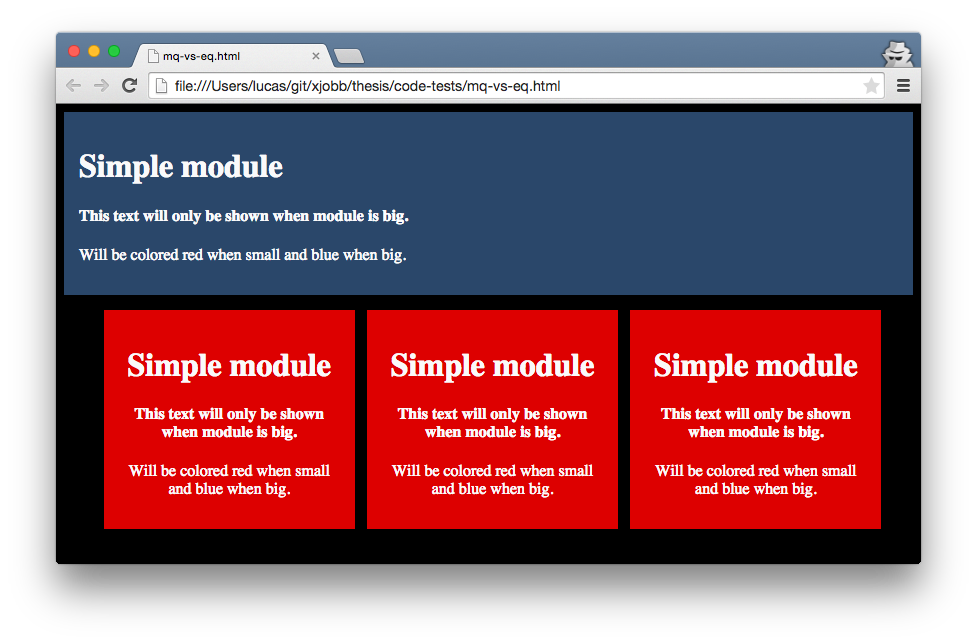
\includegraphics[width=\linewidth]{images/eq-big}
          \end{minipage}%
          \caption{
            The desired behavior is that the small module instances should be colored red since their widths are narrow, and the big instance should be blue since its width is wide.
          }
          \label{fig:problem-eq}
        \end{figure}

        Unfortunately, \gls{media queries} cannot be used to achieve this behavior (with the module still being \gls{encapsulated}).
        See figure~\ref{fig:problem-mq} for the actual behavior of the example page.
        As evident in the figure, the page is broken since either all instances are colored blue or red.
        This is due to \gls{media queries} only targeting the \gls{viewport}, and not the actual width given to the instances.
        \begin{figure}[ht]
          \centering
          \begin{minipage}{.5\textwidth}
            \centering
            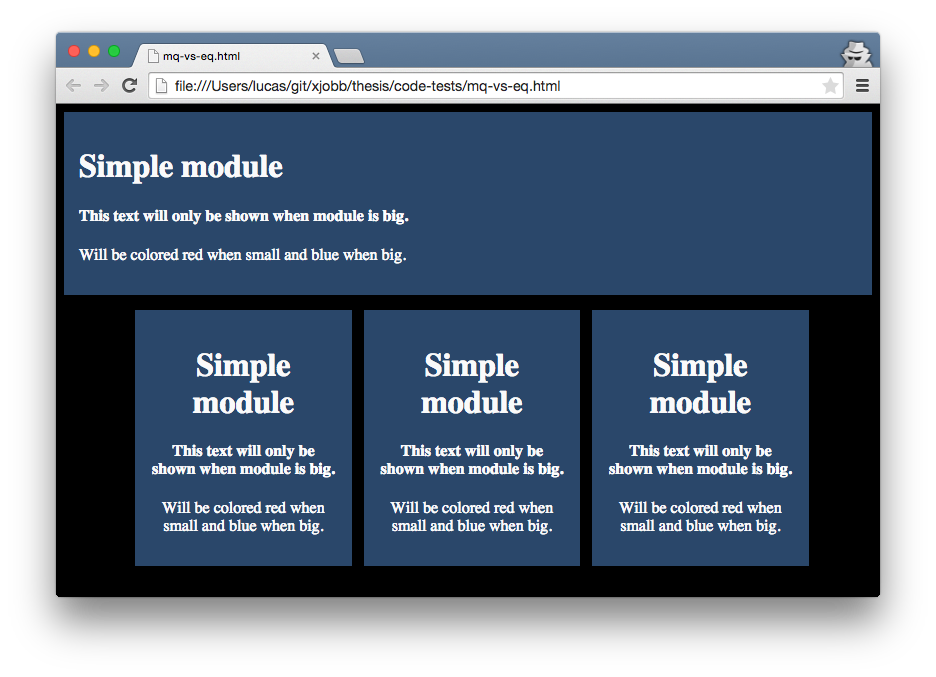
\includegraphics[width=\linewidth]{images/mq-big}
          \end{minipage}%
          \begin{minipage}{.5\textwidth}
            \centering
            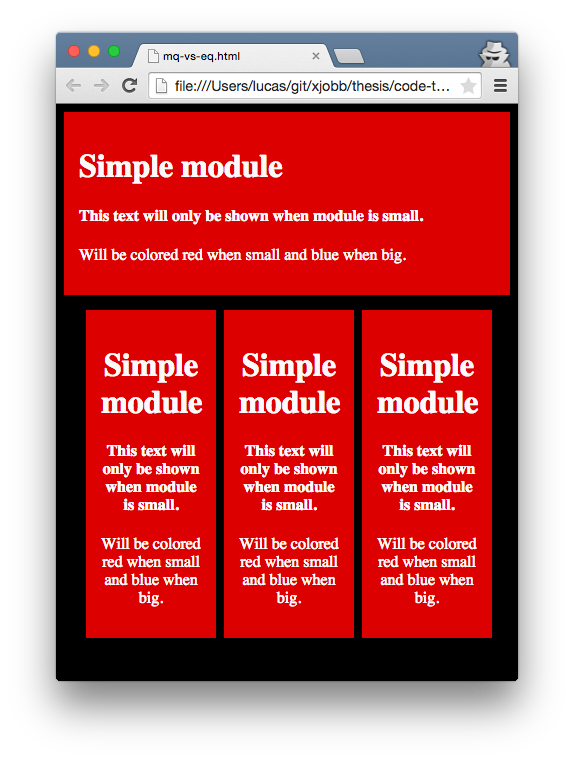
\includegraphics[width=\linewidth]{images/mq-small}
          \end{minipage}
          \caption{
            The module instances of the page do not behave as desired because they are conditionally styled by the \gls{viewport} width, which does not reflect the individual width of the instances.
            All instances are always either colored blue or red, depending on the \gls{viewport} width.
            In the left figure, the \gls{viewport} is wide and therefore all instances are colored blue.
            In the right figure, the \gls{viewport} is narrow and therefore all instances are colored red.
          }
          \label{fig:problem-mq}
        \end{figure}

        \paragraph{The solution}
        \Gls{responsive} modules should be able to react and change style by their own size, not the \gls{viewport} size.
        An identified solution to this is element queries, which allows conditional styles to be applied by \gls{element} criteria.
        The last couple of years a lot of articles have been written about the problem and how badly \gls{web} developers need element queries \cite{eq_article_localised-css,eq_article_backalley,eq_article_mqhack,eq_article_tabatkjr,eq_article_filament,eq_article_tyson,eq_article_neal,eq_article_css-tricks,eq_article_hugo,eq_article_fremycompany,eq_article_discource,eq_article_matt}.
        As stated in Section~\ref{sec:problem}, \gls{third-party} non-\gls{native} implementation efforts have been made with moderate success.
        The \gls{W3C} receives requests and questions about it, and the \gls{RICG} have started writing a draft \cite{ricg_draft} about element queries use cases.
        \todo{Should this really be here? Taken from the intro... Maybe it should stay there.}

    %%%%%%%%%%%%%%%%%%%%%%%%%%%%%%%%%%%%%%%%%%%%%%%%%%%%%%%%%%%%%%%%%%%%%%%%%%%%%%%%%%%%%%%%%%%%%%%%%%%%%%%%%%%%%%%%%%%%%%%%%%%%%%%%%%%%%%%%%%%%%%%%%%%%%%%%%%%%%%%%%%%%%%%%%%%%%%%%%%%%%%%%%%%%%%%%%%%%%%%%%%%%%%%%%%%%%%%%%%%%%%%%%%%%%%%%%%%%%%%%%%%%%%%%%%%%%%%%%%%%%%%%%%%%%%%%%%%%%%%%%%%%%%%%%%%%%%%%%%%%%%%%%%%%%%%%%%%%%%%%%%%%%%%%%%%%%%%%%%%%%%%%%%%%%%%%%%%%%%%%%%
    %%%%%%%%%%%%%%%%%%%%%%%%%%%% Layout engines
    %%%%%%%%%%%%%%%%%%%%%%%%%%%%%%%%%%%%%%%%%%%%%%%%%%%%%%%%%%%%%%%%%%%%%%%%%%%%%%%%%%%%%%%%%%%%%%%%%%%%%%%%%%%%%%%%%%%%%%%%%%%%%%%%%%%%%%%%%%%%%%%%%%%%%%%%%%%%%%%%%%%%%%%%%%%%%%%%%%%%%%%%%%%%%%%%%%%%%%%%%%%%%%%%%%%%%%%%%%%%%%%%%%%%%%%%%%%%%%%%%%%%%%%%%%%%%%%%%%%%%%%%%%%%%%%%%%%%%%%%%%%%%%%%%%%%%%%%%%%%%%%%%%%%%%%%%%%%%%%%%%%%%%%%%%%%%%%%%%%%%%%%%%%%%%%%%%%%%%%%%%
    \section{Layout engines}\label{sec:layout-engines}
      In order to understand how element queries affect \glspl{layout engine}, it is important to understand how \glspl{layout engine} operate.
      \todo{Also in order to understand how to optimize the library tasks.}
      Only the \gls{layout engine} of the \gls{browser} will be of importance, since element queries do not affect any other \gls{browser} subsystem.
      This section will give a brief explanation of the layout process that the engines generally perform, along with some usual optimizations that are performed to speed up the process.
      The render process will not be described, as it is not relevant for element queries.

      Section~\ref{sec:layout-engine-reference} to Section~\ref{sec:layout-process} describes briefly how \glspl{layout engine} operate and also presents key \gls{layout engine} concepts.
      The role of the \gls{layout engine} and reference architecture for \glspl{browser} is also presented.
      \todo{Write that the layout queue is described, which will be important to understand for the optimizations done in the library.}
      Section~\ref{sec:layout-thrashing} defines \gls{layout thrashing} will presents how it can be avoided.
      Section~\ref{sec:parallel} gives insight into the current state of the research of parallelizing the layout process.

      \todo[inline]{Have an image about the layout flow somewhere?}
      \todo[inline,color=green]{Marcos: The reference architecture could be outdated since the source is very old. The XML subsystem is hardly interesting anymore.}
      \todo[inline]{Maybe move this content to an own subsection and instead write a text about why this section is here, what the goal is (to understand parallelization and \gls{layout thrashing}), etc.}
      
      \subsection{Reference architecture}\label{sec:layout-engine-reference}
        \Glspl{browser} are complex applications that consist of many subsystems.
        Reference architecture of \glspl{browser} has been presented by \cite{browser_architecture}, see figure~\ref{fig:browser_architecture}.
        \begin{figure}[ht]
          \centering
          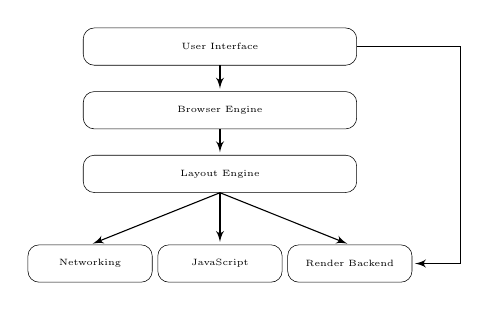
\begin{tikzpicture}[node distance=1cm, auto, transform shape, scale=0.66]  
          \tiny
            \tikzset{
                mynode/.style={rectangle,rounded corners,draw=black, top color=white, bottom color=white,very thin, inner sep=1em, minimum size=3em, text centered},
                myarrow/.style={->, >=latex', shorten >=1pt, thin},
                mylabel/.style={text width=3em, text centered}
            }  
            \node[mynode, text width=20em] (ui) {User Interface};  
            \node[mynode, text width=20em, below=0.5cm of ui] (browser-engine) {Browser Engine};
            \node[mynode, text width=20em, below=0.5cm of browser-engine] (layout-engine) {Layout Engine};
            % \node[below=of layout-engine] (dummy) {};
            \node[mynode, text width=8em, below=of layout-engine, below=of layout-engine] (javascript) {\gls{JavaScript}};
            \node[mynode, text width=8em, below=of layout-engine, left=0.1cm and 0.1cm of javascript] (networking) {Networking};  
            \node[mynode, text width=8em, below=of layout-engine, right=0.1cm of javascript] (render-backend) {Render Backend};

            \draw[myarrow] (ui.south) -- (browser-engine.north);
            \draw[myarrow] (browser-engine.south) -- (layout-engine.north);
            \draw[myarrow] (layout-engine.south) -- (networking.north); 
            \draw[myarrow] (layout-engine.south) -- (javascript.north);
            \draw[myarrow] (layout-engine.south) -- (render-backend.north);
            \draw[myarrow] (ui.east) -- +(2, 0) |- (render-backend.east);
          \end{tikzpicture} 
          \medskip
          \caption{Reference \gls{browser} architecture. The data persistence system, used by the \gls{browser} engine and the user interface, has been omitted.} 
          \label{fig:browser_architecture}
        \end{figure}
        It is shown that the \gls{layout engine} is located between the \emph{\gls{browser} engine} system and the network, \gls{JavaScript}, and display backend.
        The \gls{browser} engine acts as a high level interface to the \gls{layout engine}, and is responsible for providing the \gls{layout engine} with \glspl{URL} of content that should be fetched and rendered.
        Additionally, \gls{browser} engines usually provide the \gls{layout engine} with layout and rendering options such as user preferred font size, zoom, etc.
        The main responsibility of the \gls{layout engine} is to render the current state of the fetched \gls{hypertext} \gls{document} \cite{garsiel2011browsers}.
        The \gls{layout engine} also performs the parsing of \gls{HTML}.
        Since \glspl{document} may (and often do) change dynamically after parsetime it is important to keep in mind that the job of the \gls{layout engine} is continuous, and is not a one time operation.
        In short, \glspl{layout engine} perform four distinct tasks:
        \begin{enumerate}
          \item Fetch content (typically \gls{HTML}, \gls{CSS} and \gls{JavaScript}) and parse it in order to construct a \gls{DOM} tree. \todo{Explain DOM before this?}
          \item Construct a \gls{render tree} of the \gls{DOM} tree.
          \item Layout the \glspl{element} of the \gls{render tree}.
          \item Render the \glspl{element} of the \gls{render tree}.
        \end{enumerate}
        See Section~\ref{sec:dom-tree} and Section~\ref{sec:render-tree} for a more in-depth explanation of \gls{DOM} and \glspl{render tree}.
        \Glspl{browser} can typically display multiple pages at the same time (by using tabs, multiple windows or frames) where each page has an instance of the \gls{layout engine}.

        There are four \glspl{layout engine} that the major \glspl{browser} use, as presented in table~\ref{table:layout_engines}.
        Since \gls{Blink} is a recent \gls{fork} of \gls{WebKit} they have been grouped together as \gls{WebKit}-based \glspl{layout engine}.
        This results in three distinct \glspl{layout engine} to consider: \gls{WebKit}, \gls{Gecko} and \gls{Trident}.
        Due to \gls{Trident} being closed source, only the \gls{WebKit}-based \glspl{layout engine} and \gls{Gecko} will be considered in this section.
        \todo{Maybe not group WebKit and \gls{Blink} together, as they perform very differently in the erd tests?}

        \begin{table}[ht]\center
          \tiny
          \begin{minipage}[t]{0.38\linewidth}
            \begin{tabular}[t]{ l l l }
              \textbf{Engine} & \textbf{Browsers} & \textbf{Share} \\
              \hline
              \gls{Blink} & Chrome, Opera & 44.38\% \\
              \gls{WebKit} & Safari & 17.64\% \\
              \gls{Trident} & Internet Explorer & 14.96\% \\
              \gls{Gecko} & Firefox & 12.83\% \\
            \end{tabular}
          \end{minipage}
          \hspace{0.1cm}
          \begin{minipage}[t]{0.42\linewidth}
            \begin{tabular}[t]{ l l l }
              \textbf{Engine} & \textbf{Browsers} & \textbf{Share} \\
              \hline
              \gls{WebKit} & Safari, Chrome, Opera & 62.02\% \\
              \gls{Trident} & Internet Explorer & 14.96\% \\
              \gls{Gecko} & Firefox & 12.83\% \\
            \end{tabular}
          \end{minipage}
          \caption{
            The major \glspl{layout engine} and \glspl{browser} with market shares.
            The table to the right has grouped together \gls{Blink} into \gls{WebKit} since it is a recent for of \gls{WebKit}.
            See Section~\ref{sec:layout_engines_market_share} for more information how the market share data was gathered.}
          \label{table:layout_engines}
        \end{table}
        \todo[inline]{Remove decimals of percentages since they are estimated?}

        %The content fetching and parsing is an advanced topic by itself, but is not relevant for element queries since they impose no fundamental changes to process.
        %Also, rendering the final layout with the render backend is not affected by element queries.
        %The construction of 

      \subsection{Constructing DOM trees}\label{sec:dom-tree}
        This section is mainly based on \normalfont{\cite{w3c_dom,garsiel2011browsers,w3c_css21,w3c_html}}.
        \todo{Should it be like this?}

        The \gls{DOM} defines a platform-neutral model for events and node trees, which is used for representing and interacting with \glspl{document}.
        The \gls{DOM} provides an interface for programs (\gls{JavaScript} in the \gls{browser}) to access and mutate the structure, style, and content of \glspl{document}.
        \Glspl{element} of the \gls{document} are converted to \gls{DOM} nodes, and therefore the whole \gls{document} is represented as a tree structure of \gls{DOM} nodes which is referred to as the \gls{DOM} tree.

        \Glspl{layout engine} construct \gls{DOM} trees by parsing \gls{HTML} with any included \gls{CSS} and \gls{JavaScript}.
        Parsing of \gls{HTML} is not an easy task, partly because it is expected (although not required) of \glspl{layout engine} to be forgiving of errors, such as handling malformed \gls{HTML}.
        As \gls{CSS} and \gls{JavaScript} are stricter, their grammar can be expressed in a formal syntax and can therefore be parsed with a context free grammar parser.
        Another big quirk to parsing \gls{HTML} is that it is reentrant that means that the source may change during parsing, see listing~\ref{code:reentrant-html}.
        Script \glspl{element} are to be executed synchronously when encountered by the parser.
        If such script mutates the \gls{DOM}, then the parser will need to evaluate the changes made by the script and update the \gls{DOM} tree.
        External scripts need to be fetched in order to be executed, which halts the parsing unless the script \gls{element} states otherwise.
        It should be noted that although \gls{DOM} nodes do include a \code{style} property, the \gls{CSS} cascade does not affect the nodes in the \gls{DOM} tree, and the style properties do not represent the final style of the \gls{element}.
        Instead, for scripts to obtain the final computed style for an \gls{element} special functions needs to be called (e.g. \code{getComputedStyle} in \gls{JavaScript}\footnote{See \url{http://dev.w3.org/csswg/cssom/\#dom-window-getcomputedstyleelt-pseudoelt} for details about the function.}).
        Since externally linked \gls{CSS} \glspl{document} do not directly affect the \gls{DOM} tree they could conceptually be fetched and parsed after the parsing of the \gls{HTML}.
        However, scripts can request the computed style of \gls{DOM} nodes and therefore either the parsing of \gls{HTML} needs to be halted in order to fetch and parse \gls{CSS} when needed, or the scripts accessing style properties of \gls{DOM} nodes need to be halted.
        A common optimization is to use a speculative parser that continues to parse the \gls{HTML} when the main parser has halted (for executing scripts usually).
        The speculative parser does not change the \gls{DOM} tree, instead it searches for external resources that can be fetched in parallel while waiting for the main parser to continue.

        \begin{lstlisting}[gobble=10,caption={Simple example of reentrant HTML. The \gls{layout engine} needs to reconstruct the \gls{DOM} tree after executing the \gls{JavaScript}. The page will not be rendered until all \gls{JavaScript} has been executed.}, captionpos=b, label={code:reentrant-html}]
          <html>
            <body>
              <div id="container">
                <p id="tip">When in doubt, mumble.</p>
              </div>
              <script>
                var container     = document.getElementById("container");
                var tip           = document.getElementById("tip");
                var intro         = document.createElement("h4");
                intro.innerHTML   = "A tip:";
                container.insertBefore(intro, tip);
              </script>
            </body>
          </html>
        \end{lstlisting}

        \todo[inline]{Philipp: A picture of the DOM corresponding to some HTML would be good.}
        \todo[inline]{Write about media type, and how the CSS is calculated if it is in this stage?}

      \subsection{Render trees}\label{sec:render-tree}
        When the \gls{DOM} tree has been constructed and all external \gls{CSS} has been fetched and parsed, it is time for the \gls{layout engine} to create the \gls{render tree}.
        This section is mainly based on \normalfont{\cite{garsiel2011browsers,w3c_css21}}.

        A \gls{render tree} is a visual representation of the \gls{document}.
        In contrast to the \gls{DOM} tree, the \gls{render tree} only contains \glspl{element} that affect the rendered result in any way.
        The nodes of the \gls{render tree} are called \emph{renderers} (also known as \emph{frames} or \emph{render objects}), as the nodes are responsible for their own and all subnodes layout and rendering.
        In order to know how to render them, the final style of each renderer needs to be computed which is done by the \gls{layout engine} while constructing the tree.
        Each renderer represents a rectangle (with a size and position) with a given style.
        There are different types of renderers, which affect how the renderer rectangle is computed.
        The type can be directly affected by the \code{display} style property.

        Typically nodes of the \gls{DOM} tree have a 1:1 relation to nodes of the \gls{render tree}, but the relation can also be smaller or larger.
        Since the \gls{render tree} only contains nodes that affect the rendered result, nodes that do not affect the layout flow of the \gls{document} and that aren't visible will not be present in the \gls{render tree}.
        For instance, a \gls{DOM} node with the \code{display} property set to \code{none} will have the relation 1:0 (it will not be present in the \gls{render tree} because it is not visible and will not affect the layout flow).
        It should be noted that nodes with the \code{visibility} style property set to \code{hidden} will be present in the \gls{render tree}, although they are not visible, since they still affect the layout flow.

        Even though all style properties have been resolved for each node in the \gls{render tree} (through \gls{CSS} cascading), the renderers still do not know about the size and position of their rectangles.
        This is because some properties depend on the flow of the \gls{document}, which cannot be resolved by style cascading and this need to be computed through a layout.
        The layout process will resolve the final position and size of all renderers.

      \subsection{Style computation}\label{sec:style-computation}
        Both the \gls{render tree} and scripts need to be able to get the final style of \glspl{element}.
        In this section a brief explanation of selector matching, style cascading, inheritance and rule set weighting is given.
        \gls{CSS} property definitions will also be described.
        This section is mainly based on \normalfont{\cite{garsiel2011browsers,w3c_css21,w3c_css_style_attr}}.

        To trace how the style of an \gls{element} is computed can be a complex task, since there are many parameters to \gls{element} style computations.
        First, styles for an \gls{element} can be defined in several places:
        \begin{enumerate}
          \item In the default styles of the \gls{browser}.
          \item In the user defined \gls{browser} style.
          \item In external \gls{CSS} \glspl{document}.
          \item In internal \gls{CSS} \code{style} tags in the \gls{document} head.
          \item In inline \gls{CSS} in the \code{style} \gls{element} attribute.
          \item In scripts modifying the \gls{element} style through the \gls{DOM} tree.
          \item In special attributes of the \gls{element} such as \code{bgcolor} (deprecated, but possible).
        \end{enumerate}
        This can be grouped into author, user and \gls{browser} styles.
        \todo{Clarify this.}
        The four first items have in common that they are \emph{cascading} their style rules through \emph{selector matching}, and may define rule sets.
        Selector matching conceptually finds all \glspl{element} in the \gls{DOM} tree that matches a \gls{CSS} selector, to apply style declarations of the rule set.
        The rule sets are weighted so that if a property is assigned values by multiple rule sets the one with highest weight will be applied.
        The weighting process starts with the origin of the style:
        \begin{itemize}
          \item In case of normal rule declarations, the style weighting relation is: $browser < user < author$.
          \item Important rule declarations have the following relation: $author < user$.
        \end{itemize}
        The weighting process continues by calculating the \gls{specificity} of all rule set selectors, the higher the \gls{specificity} the higher the rule set will be weighted.
        This will make rule sets with more specific selectors override rule sets with more general selectors.
        Finally, if two rule declarations have the same weight, origin and \gls{specificity} the rule set specified last will win.
        Inline \gls{CSS} does not cascade since all rules given are automatically matched with the \gls{element} of the style attribute.
        However, inline \gls{CSS} is considered with highest possible \gls{specificity} when performing the style cascade.
        It is important to note that the styling methods number five and six are conceptually the same, since they both alter the style property of the \gls{DOM} representation of the \gls{element}.
        The last styling method, using special style attributes, is deprecated and all styles applied this way are weighted as low as possible.

        If the cascade results in no value for an \gls{element} style property, then the property can \emph{inherit} a value or have an initial value defined by the \gls{CSS} \emph{property definition}.
        Property definitions describe how the style properties should behave; see table~\ref{table:css_property_definition} for the format of property definitions.
        For instance, the \code{width} property definition states that legal values are absolute lengths, percentages or \code{auto} (which will let the \gls{browser} decide).
        The percentages are relative to the containing block.
        The initial value is \code{auto}, the properties applies to all non-replaced inline \glspl{element}, table rows and row groups.
        The value may not be inherited, and the media group is \code{visual}.
        The computed value is either the absolute length, calculated percentage of the containing block or what the \gls{browser} decides (in case of \code{auto}).
        If a property may inherit values, it will inherit the value of the first ancestor that has a value that is not \code{inherited}.

        \begin{table}[ht]\center
          \tiny
          \begin{tabular}[t]{ r | l }
            \textbf{Value} & Defines the legal values and the syntax. \\
            \textbf{Initial} & The initial value that the property will have. \\
            \textbf{Applies to} & The \glspl{element} that the property applies to. \\
            \textbf{Inherited} & Determines if the value should be inherited or not. \\
            \textbf{Percentages} & Defines if percentages are applicable, and how they should be interpreted. \\
            \textbf{Media} & Defines which media group the property applies to. \\
            \textbf{Computed value} & Describes how the value should be computed. \\
          \end{tabular}
          \caption{The \gls{CSS} property definition format that describes how all \gls{element} style properties behave.}
          \label{table:css_property_definition}
        \end{table}

        This process will resolve most style properties, but as stated in Section~\ref{sec:render-tree} some properties require a layout in order to be resolved.

        \todo[inline]{Explain the syntax of CSS?}

      \subsection{The layout process}\label{sec:layout-process}
        When the \gls{render tree} has been constructed, and the style properties have been resolved for all nodes, it is time to perform the actual layout \cite{garsiel2011browsers}.
        The layout process will decide the final computed style of all \glspl{element}, and needs to be done before rendering.
        \gls{HTML} is flow based, which means that a \gls{document} layout (also known as a \emph{reflow}) can generally be performed top to bottom and left to right in one pass.
        This is possible because the geometry of \glspl{element} typically do not depend on the siblings or children\todo{Seems weird to say that flow is not dependent on children, since the height is propagated upwards.}.
        Layout is performed recursively by starting at the root of the tree, let the renderer render itself and all of its children which will render themselves and their children and so on.
        When a layout is performed on the whole \gls{render tree} it is called a \emph{global layout}.
        To avoid global layouts when a renderer has been changed, a dirty bit system is usually implemented.
        The system marks which renderers in the tree that need a layout, which avoids layout of unaffected \glspl{element}.
        Layouts that only layout the dirty renderers are called \emph{incremental layouts}.
        A \gls{layout engine} that uses the dirty bit system usually keeps a queue of incremental layout commands.
        The scheduler system later triggers a \glslink{batch processing}{batch execution} of the incremental layout commands asynchronously.
        A global layout is triggered when the \gls{viewport} is resized or when styles that affect the whole \gls{document} is changed (such as \code{font-size}).
        Because the \gls{API} of \code{getComputedStyle} promises resolved values for all style properties, calling the function forces a full layout (flushing the incremental layout commands queue).
        When a renderer performs a layout the following usually happens:
        \begin{enumerate}
          \item The own width of the renderer is determined.
          \item The renderer positions all children and requests them to layout themselves (with given position and width).
          \item The heights, margins and paddings of the children are accumulated in order to decide the own height of the renderer.
        \end{enumerate}
        Of course, only the children that need a layout will be affected (dirty, or global layout) in step 2.
        So, the widths and positions are sent down in the tree and the heights are sent up in the tree in order to construct the final layout.

        The widths are calculated by the \code{width} style of the \glspl{element}, relative to the container \gls{element} width.
        Margins and paddings are also taken into account when calculating the widths.
        When the width of an \gls{element} is calculated, it needs to be controlled against the \code{min-width} and \code{max-width} style properties and make sure that the width is inside the given range.
        If the content of an \gls{element} does not fit with the calculated width (text usually needs to perform line break when the width is too small), the \gls{element} needs to break up the content into multiple renderers in order to expand the height.
        The renderer that has decided that it needs to break the content up into multiple renderers propagates to the parent renderer that it needs to perform the breaking.
        When the parent renderer has created the renderers needed to fit the content with the given height, layout is performed on the new renderers and then the final height can be calculated and propagated upwards.
      
      \subsection{Layout thrashing and how to avoid it}\label{sec:layout-thrashing}
        Recall from section \ref{sec:layout-process} that \glspl{layout engine} store incremental layout commands in a queue in order to \glslink{batch processing}{batch process} layouts.
        \todo{Perhaps remove this, as the reader is supped to just have read it.}
        The term \gls{layout thrashing} refers to when the layout queue repeatedly is being flushed by scripts; forcing the \gls{layout engine} to perform multiple independent layouts that could have in theory been \glslink{batch processing}{batch processed}.
        Layouts are \emph{thrashed} since the \gls{layout engine} usually needs to perform layout on the whole subtree of the affected element for each incremental layout command, hence thrashing most of the work it did the previous layout command.
        See listing~\ref{code:thrashing-example} for an example of \gls{JavaScript} code that results in \gls{layout thrashing}.
        \begin{lstlisting}[gobble=10,caption={Example of \gls{layout thrashing}. The code reads and doubles the widths of 1000 \glspl{element} in \textasciitilde700 ms. The \code{parseSize} function is not important to understand the example.}, captionpos=b, label={code:thrashing-example}]
          /* Doubles the width of each element in the elements collection parameter. */
          function doubleWidths(elements) {
            elements.forEach(function readWriteWidth(element) {
              var width = parseSize(getComputedStyle(element).width);
              element.style.width = width * 2 + "px";
            });
          }

          // 1000 div elements as only children of a div container.
          var elements = [...];
          doubleWidths(elements); // ~700 ms
        \end{lstlisting}
        For each element given as parameter to the \code{doubleWidths} function, the \code{readWriteWidth} function is called with an element as argument.
        In that function, the computed style of the element is requested, which will force a style computation for that \gls{element}.
        If any \gls{DOM} node affecting the element is marked as dirty, a layout will also need to be performed before returning the computed style of the \gls{element}.
        When the computed style has been acquired, the width of the \gls{element} is set to a new value, which is a \gls{DOM} mutation that will need to be synchronized with the \gls{render tree}.
        Therefore, the element and its ancestors will be marked as dirty.
        The next time \code{getComputedStyle} is called, which happens when processing the next element in the collection, a layout will be forced since \gls{DOM} nodes that affects the \glspl{element} has been marked as dirty.
        See figure~\ref{fig:layout-thrashing-example-1} for a visualization of the execution of the \code{doubleWidths} function.
        It is shown in the figure that style computations and layout is performed in each iteration.
        The total time spent on style computations is \textasciitilde40 ms and layout is \textasciitilde600 ms, which leaves \textasciitilde60 ms for the actual script execution.

        \begin{figure}[ht]
          \centering
          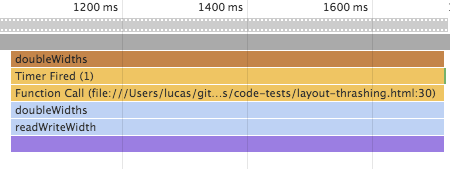
\includegraphics[scale=0.7]{images/layout-thrashing-example-1-big}
          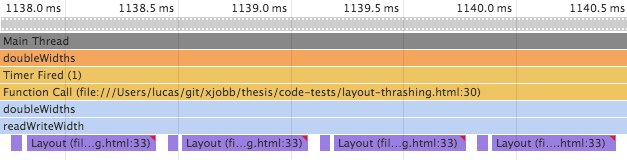
\includegraphics[scale=0.6]{images/layout-thrashing-example-1}
          \caption{Two timeline figures of executing the example code given in listing~\ref{code:thrashing-example}. Both figures show the same timeline, where the top figure shows the whole execution and the bottom only shows a small section of the execution. Notice that they do not share the same time axis. Here it is clear that \gls{layout thrashing} occurs, since layout is being done repeatedly throughout the whole execution (each iteration in the loop).}
          \label{fig:layout-thrashing-example-1}
        \end{figure}
        
        To avoid \gls{layout thrashing}, the computed style requests and \gls{DOM} mutations need to be performed in \glslink{batch processing}{batches}, as presented in listing~\ref{code:thrashing-example-fixed}.
        While it is algorithmically inefficient to iterate over the same collection twice --- the \glslink{batch processing}{batched} approach executes \textasciitilde100 times faster than the original version.
        \begin{lstlisting}[gobble=10,caption={Example of avoiding \gls{layout thrashing} by \gls{batch processing} reads and writes to the \gls{DOM}. The code reads and double the widths of 1000 \glspl{element} in \textasciitilde7 ms.}, captionpos=b, label={code:thrashing-example-fixed}]
          /* Doubles the width of each element in the elements collection parameter. */
          function doubleWidths(elements) {
            var widths = [];

            // First retrieve all element widths.
            elements.forEach(function getWidths(element) {
              var width = parseSize(getComputedStyle(element).width);
              widths.push(width);
            });

            // Then mutate the DOM with the new widths.
            elements.forEach(function writeWidths(element, index) {
              element.style.width = widths[index] * 2 + "px";
            });
          }

          // 1000 div elements as only children of a div container.
          var elements = [...];
          doubleWidths(elements); // ~7 ms
        \end{lstlisting}
        Now, the \code{doubleWidths} function performs two \glslink{batch processing}{batches} that both iterates over the \glspl{element} collection.
        In the first \glslink{batch processing}{batch}, all widths of all \glspl{element} are acquired and stored in a collection.
        Since no \gls{DOM} mutation occurs in the first \glslink{batch processing}{batch}, the \gls{layout engine} does not need to perform any layout while retrieving the styles.
        In the second \glslink{batch processing}{batch}, all \glspl{element} are assigned the new widths based on the widths retrieved in the first \glslink{batch processing}{batch}.
        Since the script does not read the \gls{DOM} in any way during in the second \glslink{batch processing}{batch}, all \gls{DOM} mutations can be queued by the \gls{layout engine} to be \glslink{batch processing}{batch} processed.
        See figure~\ref{fig:layout-thrashing-example-1-fixed} for a visualization of the execution of the \glslink{batch processing}{batched} example version.
        In the figure, it is clear that the \gls{layout engine} is able to first execute the \gls{JavaScript}, and later perform all style and layout computations in a \glslink{batch processing}{batch}.
        \begin{figure}[ht]
          \centering
          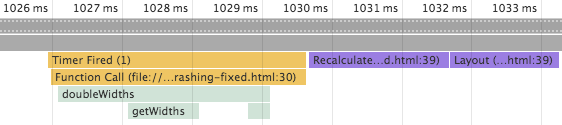
\includegraphics[scale=0.7]{images/layout-thrashing-example-1-fixed}
          \caption{A timeline of executing the example code given in listing~\ref{code:thrashing-example-fixed}. It is clear in the figure that \gls{layout thrashing} does not occur, since all style computations and layout is performed in a \glslink{batch processing}{batch} after that the example code has finished executing.}
          \label{fig:layout-thrashing-example-1-fixed}
        \end{figure}

        The total time spent on style computations has been reduced to \textasciitilde2 ms, layout to \textasciitilde1.5 ms, and the actual script execution to \textasciitilde3.5 ms.
        It should be noted that both versions recalculate styles for the same number of \glspl{element}, from now on denoted by $n$.
        Pausing the \gls{JavaScript} context and switching the \gls{layout engine} to style computation mode causes an overhead cost, from now on denoted by the constant $O_{s}$.
        Let $C_{s}$ denote the time it takes for the \gls{layout engine} to calculate the style of one \gls{element}, then the total time needed for style computations in the first version is given by $T(n) = n(O_s + C_s)$.
        Since the second version enabled the \gls{layout engine} to calculate the style of all \glspl{element} in a \glslink{batch processing}{batch}, the total time needed was reduced to $T(n) = nC_s + O_s$.
        The style computation was reduced from \textasciitilde40 ms to \textasciitilde2 ms because the second version avoids $n - 1$ overhead costs.
        However, it should be noted that both versions have time complexity $O(n)$.
        
        The major part of the time reduction is due to the layout time being significantly reduced.
        The reason why the layout time was significantly reduced is because the two versions do not perform layout on the same amount of \glspl{element}.
        When an element and its ancestors has been marked as dirty, a layout will need to be performed on the subtree which contains at least all $n$ \glspl{element} and possibly some ancestor \glspl{element}.
        So the minimum number of nodes that need to be laid out is given by $n + n_{a}$, where $n_a$ is the number of ancestor \glspl{element}.
        Since the first version forces the \gls{layout engine} to perform a layout in each iteration, the minimum number of \glspl{element} laid out is given by $n(n + n_a)$.
        Similar to style computation, performing a layout also has an overhead cost $O_{l}$.
        Let $C_{l}$ denote the time it takes for the \gls{layout engine} to layout one \gls{element}, then the total time needed for layout in the first version is given by $T(n) = n(O_{l} + C_{l}(n + n_a))$.
        The second version enables the \gls{layout engine} to \glslink{batch processing}{batch process} the \gls{DOM} manipulations, and therefore only one layout of the subtree will need to be performed, which results in the minimum number of \glspl{element} laid out being $n + n_a$.
        The total time needed for layout in the second version is then given by $T(n) = O_{l} + C_{l}(n + n_a)$.
        The first version has time complexity $O(n^2)$ while the second version has time complexity $O(n)$, which is a significant optimization.

        \todo[inline]{Explain that the script execution time was probably reduced due to avoiding n-1 context switches between the JS engine and the \gls{layout engine}?}
        \todo[inline]{Analyze the numbers to give some rough numbers on overhead and cost times?}
        \todo[inline]{Explain that $n_a$ is not a parameter to the T function?}
        \todo[inline]{Refer to some section in the appendix for how to read the timeline images? Philipp said that I should try to explain it very briefly in this section.}
        \todo[inline]{Sources?}

      \subsection{Parallelization}\label{sec:parallel}
        No longer can performance of an application increase over time without any code changes (as opposed to the times when the \gls{CPU} clock speeds increased rapidly) \cite{parallelizing_the_web_browser}.
        Now, applications need to utilize the multiple cores of the \gls{CPU} instead of relying on high clock speed.
        Parallelization is something \gls{layout engine} vendors are interested in, and research is being done about utilizing multiple cores to increase the performance of the engines.
        In this section a small summary will be given about the current research front, and how the parallelization of \glspl{layout engine} can be approached.
        \todo{Check so that the section actually does what the meta says}

        As \gls{web} applications grow bigger and more demanding, \glspl{browser} continuously need to improve the performance on all levels \cite{parallelizing_the_web_browser}.
        Fetching resources over the network is the only thing that is done in parallel today.
        The rest of the \gls{browser} system is designed and optimized to run sequentially \cite{zoomm}.
        On computers, \glspl{browser} usually achieve parallelism by running each page context in parallel (each tab and window of the \gls{browser} runs in a separate process) \cite{fan2011optimizing,zoomm}.
        This approach is appealing because it utilizes the cores of the machine by still having all subsystems run sequentially for each page, while improving the overall performance of the \gls{browser}.
        However, this approach is not enough as the page performance is not improved if only one page is present.
        For the \gls{web} to be a true competitor to heavy \gls{native} applications\todo{Reformulate to not use the word native.}, the page performance needs to be increased (not only the overall \gls{browser} performance).
        It is then important to be able to dedicate multiple cores to one page instead of having all the pages present using their own core (perhaps all non-visible pages can share one core while the main visible page can have access to multiple cores if needed).
        Also, with the number of mobile devices browsing the \gls{web} increasing rapidly it is important to be able to achieve good parallelism \cite{meyerovich2010fast,parallelizing_the_web_browser}.
        Light devices such as small laptops, mobile phones and tablets share a common goal --- they want to reduce power consumption while increasing the performance.
        This can be achieved with multicore processors that run at lower clock speeds.
        \todo{Write that many cores is preferred over high clock speed? Why?}
        It has been shown that the performance of mobile \glspl{browser} is \gls{CPU} bound contrary to the common belief that they are network bandwidth bound \cite{parallelizing_the_web_browser,meyerovich2010fast}.
        This is why many researchers target light devices when trying to parallelize \gls{web} \glspl{browser}.
        Of course, once the methods have matured and been implemented, desktop \glspl{layout engine} will benefit from parallelization as well.

        \gls{CSS} selector matching is a good candidate for parallelization, due to matching nodes to selectors being independent from other selector matches.
        A successful parallelization of selector matching has been achieved with locality-aware task parallelism \cite{parallelizing_the_web_browser}.
        It has also been shown that selector matching and style resolving (through cascading) can be parallelized \cite{zoomm}.
        It is possible to resolve \gls{element} styles in parallel as long as two requirements are fulfilled: the matching task must have finished for the \gls{element} to resolve styles for, and the parent \gls{element} must have resolved all styles (since the \gls{element} might inherit some styles from the parent).
        As long as these requirements are fulfilled, selector matching and style resolving can run in parallel for different \glspl{element}.
        The layout process can also be parallelized, since the layout process has been shown to be subtree independent for non-float \glspl{element} \cite{servo_parallel,servo_blog}.
        Siblings of the layout tree can be processed independently of each other (in the general case), and is suitable to parallelize with a work-stealing algorithm\footnote{See \url{http://supertech.csail.mit.edu/papers/steal.pdf} for more information about work-stealing algorithms.} \cite{meyerovich2010fast}.
        \todo[inline]{Philipp: It would be very interesting to just shortly summarize typical performance gains due to parallelization.}


  %%%%%%%%%%%%%%%%%%%%%%%%%%%%%%%%%%%%%%%%%%%%%%%%%%%%%%%%%%%%%%%%%%%%%%%%%%%%%%%%%%%%%%%%%%%%%%%%%%%%%%%%%%%%%%%%%%%%%%%%%%%%%%%%%%%%%%%%%%%%%%%%%%%%%%%%%%%%%%%%%%%%%%%%%%%%%%%%%%%%%%%%%%%%%%%%%%%%%%%%%%%%%%%%%%%%%%%%%%%%%%%%%%%%%%%%%%%%%%%%%%%%%%%%%%%%%%%%%%%%%%%%%%%%%%%%%%%%%%%%%%%%%%%%%%%%%%%%%%%%%%%%%%%%%%%%%%%%%%%%%%%%%%%%%%%%%%%%%%%%%%%%%%%%%%%%%%%%%%%%%%
  %%%%%%%%%%%%%%%%%%%%%%%%%%%% Element queries
  %%%%%%%%%%%%%%%%%%%%%%%%%%%%%%%%%%%%%%%%%%%%%%%%%%%%%%%%%%%%%%%%%%%%%%%%%%%%%%%%%%%%%%%%%%%%%%%%%%%%%%%%%%%%%%%%%%%%%%%%%%%%%%%%%%%%%%%%%%%%%%%%%%%%%%%%%%%%%%%%%%%%%%%%%%%%%%%%%%%%%%%%%%%%%%%%%%%%%%%%%%%%%%%%%%%%%%%%%%%%%%%%%%%%%%%%%%%%%%%%%%%%%%%%%%%%%%%%%%%%%%%%%%%%%%%%%%%%%%%%%%%%%%%%%%%%%%%%%%%%%%%%%%%%%%%%%%%%%%%%%%%%%%%%%%%%%%%%%%%%%%%%%%%%%%%%%%%%%%%%%%
  \chapter{Element queries}\label{ch:eq}
    Now that a good understanding of \glspl{browser} (especially the \gls{layout engine}), \gls{responsive} design, and modular development has been acquired it is time to address element queries --- a solution to the modular \gls{responsive} \gls{web} design problem as presented in Section~\ref{sec:rwd-modular-problem}.
    
    Section~\ref{sec:eq-definitions} defines element queries, and shows how they can be used to solve the problem.
    \todo{Should it really be shown how element queries solve the problem?}
    It also presents the identified general use case for element queries.
    Since no syntax have been defined yet for element queries, pseudo-syntax is presented in this section to be used throughout this thesis.
    Some element queries terminology is also described, which is extensively used throughout this thesis.
    Section~\ref{sec:eq-problems} presents some of the problems of implementing element queries \glslink{native}{natively} in \glspl{layout engine}.
    Section~\ref{sec:eq-approaches} gives insight into some of the design approaches to element queries, as discussed by the W3C, to overcome some of the problems.

    %%%%%%%%%%%%%%%%%%%%%%%%%%%%%%%%%%%%%%%%%%%%%%%%%%%%%%%%%%%%%%%%%%%%%%%%%%%%%%%%%%%%%%%%%%%%%%%%%%%%%%%%%%%%%%%%%%%%%%%%%%%%%%%%%%%%%%%%%%%%%%%%%%%%%%%%%%%%%%%%%%%%%%%%%%%%%%%%%%%%%%%%%%%%%%%%%%%%%%%%%%%%%%%%%%%%%%%%%%%%%%%%%%%%%%%%%%%%%%%%%%%%%%%%%%%%%%%%%%%%%%%%%%%%%%%%%%%%%%%%%%%%%%%%%%%%%%%%%%%%%%%%%%%%%%%%%%%%%%%%%%%%%%%%%%%%%%%%%%%%%%%%%%%%%%%%%%%%%%%%%%
    %%%%%%%%%%%%%%%%%%%%%%%%%%%% Definitions and Usages
    %%%%%%%%%%%%%%%%%%%%%%%%%%%%%%%%%%%%%%%%%%%%%%%%%%%%%%%%%%%%%%%%%%%%%%%%%%%%%%%%%%%%%%%%%%%%%%%%%%%%%%%%%%%%%%%%%%%%%%%%%%%%%%%%%%%%%%%%%%%%%%%%%%%%%%%%%%%%%%%%%%%%%%%%%%%%%%%%%%%%%%%%%%%%%%%%%%%%%%%%%%%%%%%%%%%%%%%%%%%%%%%%%%%%%%%%%%%%%%%%%%%%%%%%%%%%%%%%%%%%%%%%%%%%%%%%%%%%%%%%%%%%%%%%%%%%%%%%%%%%%%%%%%%%%%%%%%%%%%%%%%%%%%%%%%%%%%%%%%%%%%%%%%%%%%%%%%%%%%%%%%
    \section{Definitions and Usages}\label{sec:eq-definitions}
      \todo[inline]{Might want to change title to Def and syntax, instead of usage.}
      \noindent
      Element queries are the solution to the problem of \gls{responsive} modules as described in Section~\ref{sec:rwd-modular-problem}, since they allow modules to conditionally style themselves by element criteria.
      \todo{Might wanna expand on this.}

      \Gls{media queries} and element queries are similar in the sense that they both enable developers to define conditional style rules that are applied by specified criteria \cite{w3c_css_mq}.
      The main difference is the type of criteria that can be used; in \gls{media queries} device and media criteria are used, while element criteria are used in element queries.
      It can somewhat simplified be described as that \gls{media queries} target the \gls{document} root and up (i.e., the \gls{viewport}, \gls{browser}, OS, device, input mechanisms, etc.) while element queries target the \gls{document} root and down (i.e., \glspl{element} of the \gls{document}).

      \paragraph{Terminology}
      The entity that is evaluated against a query is called the \emph{target} of the query.
      For \gls{media queries}, the target is usually the device or \gls{viewport}.
      For element queries, the target is usually an \gls{element}.
      It should be noted that the target is the entity that is evaluated against the query, and not the entity that has conditionally styles applied.
      For instance, it is not possible to conditionally style the target of \gls{media queries}, since \gls{CSS} is incapable of altering the device.
      For element queries, the target entity is sometimes referred to as the target \gls{element}.
      In the case of element queries, the target element may also be the element that has conditionally styles applied (but is generally not).
      \gls{CSS} style declarations that are applied conditionally using either element queries or \gls{media queries} are sometimes referred to as \emph{conditional style declarations} or shortened \emph{conditional styles}.
      When the \gls{layout engine} evaluates a media or element query to determine whether the selectors match or not is called \emph{query selector matching}.
      The expressions that define when different conditional style declarations should be applied are called \emph{breakpoints}.
      For instance, the \glslink{media queries}{media query} \code{@media (max-width: 500px)} selector defines one breakpoint; that the element should be styled differently depending on if it is wider than 500 pixels or not.
      There can be multiple breakpoints defined for both media and element queries.
      Element queries also define an element \emph{style state}, which is in which state the target element of an element query is in (often relative to the breakpoints).
      For instance, if an element query targets an element \code{\#foo} with a width breakpoint of 500 pixels (similar to the \glslink{media queries}{media query} example), then the target element \code{\#foo} would have two style states: narrower or wider than 500 pixels.
      The number of style states for an element of a given style property is $n + 1$ where $n$ is the number of breakpoints for that style property.

      \paragraph{Pseudo-syntax}
      As already stated, element queries are not yet standardized and the exact behavior and syntax is still undefined.
      In this thesis, the pseudo-syntax of element queries is defined as a pseudo-class named \code{eq}.
      Recall from the \gls{CSS} selectors level 3 specification \cite{w3c_css_selectors} that pseudo-classes permits selection based on extended element information, and is often described as performing selection by the state of the \gls{element}.
      The \code{eq} pseudo-class takes expressions as input, that is evaluated against the target \gls{element}, as shown in the examples given in listing~\ref{code:eq-pseudo-syntax-examples}.
      \begin{lstlisting}[gobble=8,caption={Examples of the element queries pseudo-syntax.}, captionpos=b, label={code:eq-pseudo-syntax-examples}]
        /* Matches all "a" elements that are wider than 500 pixels. */
        a:eq(width > 500px) {
          color: yellow;
        }

        /* Matches any "a" element that is a child of a p element 
           with the "foo" class that is narrower than 300 pixels. */
        p.foo:eq(width < 300px) a {
          color: red;
        }

        /* Matches any p element with the "foo" class that is wider 
           than or equal to 300 pixels that is a child of an "a" element. */
        a p.foo:eq(width >= 300px) {
          color: blue;
        }

        /* Matches any "a" element that is in the hover pseudo-class state with a
           width between 300 and 500 pixels. */
        a:hover:eq(300px <= width <= 500px) {
          color: purple;
        }
      \end{lstlisting}

      \paragraph{General use case}
      According to the draft written by the \gls{RICG} the general use case is to conditionally style an element by an ancestor \gls{element}'s width to allow \gls{responsive} \gls{web} design for reusable modules \cite{ricg_draft}.
      Pages are usually designed to grow in height when content does not fit the \gls{viewport} and therefore \gls{responsive} \gls{web} design usually targets the \gls{viewport} width for layout breakpoints \cite{book_rwd,wiki_rwd,mjelde2014performance}.
      This can be verified by viewing the source code of popular \gls{responsive} design frameworks (e.g., \gls{Bootstrap}) where almost exclusively width breakpoints are present.
      Since element queries are to mainly allow \gls{responsive} \gls{web} design for modules, the same is assumed to apply for element queries (that only the width of \glspl{element} are of interest).
      Further, it is assumed that element queries mainly target ancestor \glspl{element} of the element to be conditionally styled, and therefore it is not crucial to support element queries for the own element width.
      This implies that element queries that targets void \glspl{element} (i.e., \glspl{element} that cannot contain content) are also not crucial, and hence are not regarded as a general use case.

      \todo[inline]{Should it really also be discussed in detail how element queries solve the problem?}
      \todo[inline]{If a better example is found to be used in \ref{sec:rwd-modular-problem}, the same example can be used here and shown how element queries make it behave as expected.}

    %%%%%%%%%%%%%%%%%%%%%%%%%%%%%%%%%%%%%%%%%%%%%%%%%%%%%%%%%%%%%%%%%%%%%%%%%%%%%%%%%%%%%%%%%%%%%%%%%%%%%%%%%%%%%%%%%%%%%%%%%%%%%%%%%%%%%%%%%%%%%%%%%%%%%%%%%%%%%%%%%%%%%%%%%%%%%%%%%%%%%%%%%%%%%%%%%%%%%%%%%%%%%%%%%%%%%%%%%%%%%%%%%%%%%%%%%%%%%%%%%%%%%%%%%%%%%%%%%%%%%%%%%%%%%%%%%%%%%%%%%%%%%%%%%%%%%%%%%%%%%%%%%%%%%%%%%%%%%%%%%%%%%%%%%%%%%%%%%%%%%%%%%%%%%%%%%%%%%%%%%%
    %%%%%%%%%%%%%%%%%%%%%%%%%%%% Problems
    %%%%%%%%%%%%%%%%%%%%%%%%%%%%%%%%%%%%%%%%%%%%%%%%%%%%%%%%%%%%%%%%%%%%%%%%%%%%%%%%%%%%%%%%%%%%%%%%%%%%%%%%%%%%%%%%%%%%%%%%%%%%%%%%%%%%%%%%%%%%%%%%%%%%%%%%%%%%%%%%%%%%%%%%%%%%%%%%%%%%%%%%%%%%%%%%%%%%%%%%%%%%%%%%%%%%%%%%%%%%%%%%%%%%%%%%%%%%%%%%%%%%%%%%%%%%%%%%%%%%%%%%%%%%%%%%%%%%%%%%%%%%%%%%%%%%%%%%%%%%%%%%%%%%%%%%%%%%%%%%%%%%%%%%%%%%%%%%%%%%%%%%%%%%%%%%%%%%%%%%%%
    \section{Problems}\label{sec:eq-problems}
      One issue that hinders element queries from being implemented \glslink{native}{natively} in \glspl{browser} is that they bring problems and limitations to \glspl{layout engine}.
      It is stated on the W3C's www-style mailing list \cite{w3c_eq_mail} by Zbarsky of Mozilla, Atkins of Google and Sprehn of Google that element queries are infeasible to implement without restricting them.
      In this section the two major problems are presented: performance and circularity.

      \subsection{Performance}
        Recall from Section~\ref{sec:render-tree} that the size and position of each \gls{element} is calculated in the layout process, and cannot be determined before an actual layout has happened.
        This imposes that a layout pass needs to be performed before resolving an \gls{element}'s size.
        If element queries are present that rely on the size of \glspl{element}, the following process needs to happen:
        \begin{enumerate}
          \item A layout pass needs to be performed in order to calculate the size of the \glspl{element} targeted by element queries.
          \item The element query conditional style declarations need to be evaluated against the \glspl{element} for the element query selector matching.
          \item If the element query selector matching results in a different matching set than in step 1, the process is repeated (with the new rules applied).
        \end{enumerate}
        So, element query selector match changes result in performing another layout that discards at least a subtree of the previous layout \cite{w3c_eq_mail}.
        As already stated, this only occurs when the layout has changed in a way that changes the matches of element query selectors.
        Unfortunately, this means that if there is any matching element query selector at page load, two layout passes always needs to be performed.
        Also, it is common for internal \glspl{API} in \glspl{layout engine} to request updated \gls{element} styles that do not require a layout to resolve (non-layout properties such as \code{color} and \code{font-family}) \cite{w3c_eq_mail}.
        Since a layout of the element query selector target is required in order to resolve the correct \gls{element} style, such internal \glspl{API} would need to force a layout in order to obtain the correct \gls{element} style (even for non-layout related properties).

        As shown in Section~\ref{sec:parallel} \gls{layout engine} vendors are interested in parallelizing their engines to increase the page performance.
        Element queries limits the parallelization, as \glspl{layout engine} would not be able to layout subtrees in parallel since an \gls{element} in one subtree might affect an \gls{element} in another subtree.
        \todo[inline]{Finish this.}

      \subsection{Circularity}\label{sec:cyclic-rules}
        The most obvious occurrences of cyclic rules are when there are conflicting element queries with width criteria and width style declarations for an \gls{element}.
        See listing~\ref{code:cyclic-simple} for the perhaps simplest example of cyclic rules.
        \begin{lstlisting}[gobble=10,caption={Simple example of cyclic rules with directly conflicting width element queries criteria and declarations. Recall the element queries pseudo-syntax defined in Section~\ref{sec:eq-definitions}.}, captionpos=b, label={code:cyclic-simple}]
          #foo {
            width: 250px;
          }

          #foo:eq(width < 300px) {
            /* This rule is applied only when the width of #foo is < 300px. */
            width: 550px;
          }

          #foo:eq(width > 500px) {
            /* This rule is applied only when the width of #foo is > 500px. */
            width: 250px;
          }
        \end{lstlisting}
        The result of this is of course implementation dependent, but a probable outcome of such code is the following infinite process:
        \begin{enumerate}
          \item 
            The initial width of the \code{\#foo} \gls{element} is set to 250 pixels.
            After a layout, the \code{\#foo:eq(width < 300px)} matches and therefore the next step is~2.
          \item 
            The width of the \gls{element} is narrower than 300 pixels, so the selector \code{\#foo:eq(width < 300px)} matches.
            Note that the \code{\#foo:eq(width > 500px)} does not match, since the width is not wider than 500 pixels.
            Since the matched selector is more specific than the \code{\#foo} selector, the new width of the \gls{element} is 550 pixels.
            The next step is~3.
          \item 
            The width of the \gls{element} is wider than 500 pixels, so the selector \code{\#foo:eq(width > 500px)} matches.
            Note that the \code{\#foo:eq(width < 300px)} does not match, since the width is not narrower than 300 pixels.
            Since the matched selector is more specific than the \code{\#foo} selector, the new width of the \gls{element} is 250 pixels.
            The next step is~2.
        \end{enumerate}
        Clearly, the \gls{browser} will be stuck in an infinite layout cycle pending back and forth between step 2 and 3 (250 pixels and 550 pixels).
        One reasonable outcome of such infinite layout loop is that the \gls{layout engine} executes one layout pass and then evaluate the next set of matched selectors and so on, which leads to a functioning page but since a layout is enforced every frame, the performance impact would be significant.
        This example is somewhat similar to writing \code{while(true);} outside the scope of a generator function in \gls{JavaScript} (i.e., it locks up the main thread), which obviously is a bad idea.
        However, cyclic rules may also occur in less obvious ways.

        \paragraph{Indirect cycles}
        Indirect cyclic rules are somewhat more complex to reason about than direct cyclic rules such as the example given in listing~\ref{code:cyclic-simple}.
        For instance, if an \gls{element} matches the width of a child \gls{element}, and the child changes width depending on the parent width, a cycle might occur.
        Consider the code in listing~\ref{code:cyclic-2}.
        \begin{lstlisting}[gobble=10,caption={Example of indirect cyclic rules. Here the user (\code{\#foo}) of the module (\code{\#module}) creates cyclic rules indirectly by specifying that it should match the width of the module.}, captionpos=b, label={code:cyclic-2}]
          /* HTML */
          <div id="foo">
            <div id="module">
              <div id="child"></div>
            </div>
          </div>

          /* CSS */
          #foo {
            /* Matches the width of the child element #module. */
            display: inline-block;
          }

          #module {
            /* Matches the width of the parent element #foo. */
            width: 100%;
          }

          #child {
            width: 250px;
          }

          #module:eq(max-width: 300px) #child {
            /* This rule applies only when the width of #module is <= 300px. */
            width: 550px;
          }

          #module:eq(min-width: 500px) #child {
            /* This rule applies only when the width of #module is >= 500px. */
            width: 250px;
          }
        \end{lstlisting}
        What makes this example more complex than the previous example is that it is less obvious for developers to identify that there are cyclic rules.
        First, the problem cannot be found without considering the rule sets of both the module and the \code{\#foo} \gls{element}.
        Second, the rules of the module \glspl{element} and the rules of the \code{\#foo} \gls{element} might be separated into different parts of the stylesheet or even different stylesheets.
        Third, the user of the module must be aware of how it styles itself in order to understand the limitations it imposes.
        By adding one line to the containing element \code{\#foo} a cycle appears in another part of the application (in the module).
        A \gls{JavaScript} equivalent of this example would perhaps be \code{var bar = true; while(bar);} with the motivation that it is still obvious that it results in an infinite loop but both the loop and the variable need to be considered.
        Also, the variable assignment could happen in another part of the code.

        \paragraph{Runtime factors}
        The examples given so far have been simple, and can easily be identified as cyclic by reviewing the \gls{CSS} code.
        It would also be possible to detect the cycles by performing a static analysis of the code.
        \Glspl{browser} could do such analysis during parse time in order to warn about or handle the cycles.
        However, cycles can occur in a more complex way that cannot be detected by static analysis.
        Consider the code in listing~\ref{code:cyclic-3}.
        \begin{lstlisting}[gobble=10,caption={Example of cyclic rules that cannot be detected by static analysis.}, captionpos=b, label={code:cyclic-3}]
          /* HTML */
          <span id="foo">
            When in doubt, mumble.
          </span>

          /* CSS */
          #foo:eq(width < 300px) {
            /* This rule applies only when the width of #foo is < 300px. */
            font-size: 2em;
          }
        \end{lstlisting}
        In this example, it is impossible to deduce if the rules are cyclic by static analysis.
        A static analysis could perhaps identify that the code could potentially result in a cycle in some cases but that is also the point of the example --- it is only cyclic in some scenarios.
        The size of the \code{\#foo} element depends on the content of it (i.e., the text).
        The width of the text depends on the font size, which is inherited.
        So the width of the \code{\#foo} \gls{element} is dependent on the inherited font size.
        When the \code{\#foo} \gls{element} is below 300 pixels wide, the font size of the element is increased to \code{2em} (which is a unit that is relative to the inherited value).
        If a \code{2em} font size results in a computed font size big enough to make the \gls{element} wider than 300 pixels, the \code{\#foo:eq(width < 300px)} does not match and therefore the element has no longer font size \code{2em}.
        Since the element width is decreased below 300 pixels when the font size of \code{2em} no longer is applied, the selector matches again and therefore the rules are cyclic.
        However, in another scenario the inherited font size might not be big enough to make the \code{\#foo} element wider than 300 pixels and therefore the rules are not cycle.
        The factors that creates the cycle are the following:
        \begin{itemize}
          \item The display type of the \gls{element}
          \item The \gls{element} queries of the \gls{element}
          \item The font size value of the \gls{element}
          \item \textbf{The inherited font size of the \gls{element}}
          \item \textbf{The content of the \gls{element}}
        \end{itemize}
        The factors in bold are especially hard to reason about during static analysis, since they may depend on runtime actions and values.
        In this example the text is static but it could have been added dynamically.
        Also, the inherited font size value depends on the closest ancestor with a font size property defined.
        Since ancestors can have their font sizes defined in relative units, the dependency tree can go up to the root of the \gls{document}.
        Further, if no ancestor defines an absolute value for the font size it is up to the \gls{browser} to default to a size, which is not known by a static analyzer.
        This implies that there is no way of knowing if the cycle appears or not without actually running the code.
        It also implies that the cycle may appear in different \glspl{browser} and settings, which makes the cycle even harder to detect.

        \todo[inline]{Try to descibe a scenario where a cycle appears, that is actually a valid use case?}
        \todo[inline]{Perhaps refer to Tab's blog that states that it is often that valid use-cases are found after they have been stated useless.}
        \todo[inline]{I think there is a lot to fetch from Tab's blog regarding this: \url{http://www.xanthir.com/b4VG0} and \url{http://www.xanthir.com/b4PR0}}
        \todo[inline]{Describe that it might be decided that cycles are not to be avoided by the eq implementation; leaving it up to the user. Tab argues that it still has to be defined what the result of cycles should be. He also says that it would be better to just avoid cycles.}
        % Far worse is that the previous examples have been of the \code{while(true);} character, which gives the false hope that even though it is possible to create cycles developers would never encounter it since ``real'' code would not be close to the examples given here.
        % With the third example, this is no longer true.
        % Increasing the font size when the layout area is smaller and decreasing the font size when the layout area is bigger is something that is frequently done in \gls{responsive} \gls{web} design.
        % Typically \gls{web} site authors want the font size to increase on handheld devices, to increase the readability.
        % Of course, the numbers given in the example might not be reasonable, but in concept it is valid use case that may result in cyclic rules.

    %%%%%%%%%%%%%%%%%%%%%%%%%%%%%%%%%%%%%%%%%%%%%%%%%%%%%%%%%%%%%%%%%%%%%%%%%%%%%%%%%%%%%%%%%%%%%%%%%%%%%%%%%%%%%%%%%%%%%%%%%%%%%%%%%%%%%%%%%%%%%%%%%%%%%%%%%%%%%%%%%%%%%%%%%%%%%%%%%%%%%%%%%%%%%%%%%%%%%%%%%%%%%%%%%%%%%%%%%%%%%%%%%%%%%%%%%%%%%%%%%%%%%%%%%%%%%%%%%%%%%%%%%%%%%%%%%%%%%%%%%%%%%%%%%%%%%%%%%%%%%%%%%%%%%%%%%%%%%%%%%%%%%%%%%%%%%%%%%%%%%%%%%%%%%%%%%%%%%%%%%%
    %%%%%%%%%%%%%%%%%%%%%%%%%%%% Approaches to overcome the problems
    %%%%%%%%%%%%%%%%%%%%%%%%%%%%%%%%%%%%%%%%%%%%%%%%%%%%%%%%%%%%%%%%%%%%%%%%%%%%%%%%%%%%%%%%%%%%%%%%%%%%%%%%%%%%%%%%%%%%%%%%%%%%%%%%%%%%%%%%%%%%%%%%%%%%%%%%%%%%%%%%%%%%%%%%%%%%%%%%%%%%%%%%%%%%%%%%%%%%%%%%%%%%%%%%%%%%%%%%%%%%%%%%%%%%%%%%%%%%%%%%%%%%%%%%%%%%%%%%%%%%%%%%%%%%%%%%%%%%%%%%%%%%%%%%%%%%%%%%%%%%%%%%%%%%%%%%%%%%%%%%%%%%%%%%%%%%%%%%%%%%%%%%%%%%%%%%%%%%%%%%%%
    \section{Approaches to overcome the problems}\label{sec:eq-approaches}
      \todo[inline]{Have the meta text that is commented out, and then have subsections that describes the different approaches?}
      \todo[inline]{Write more about iframes and shadowDOM?}
        % Now that the problems of element queries have been presented, it is time to show two approaches to solve the problems.
        % The first approach limits element queries a lot, but avoids many of the problems this way while still enabling element queries for the common use case.
        % This approach has been discussed at the \gls{W3C} and the initial draft of the \gls{RICG} assumes that this is a prerequisite to a \gls{native} implementation.
        % The second approach is to provide element queries as a third-party library which operates element queries on top of the \gls{layout engine} (in JavaScript).
        % Although not a solution to the native problems, it still provides functioning unrestricted element queries while not hindering parallelization of \glspl{layout engine}.
        % However, this approach does not solve the problem of cyclic rules.
        % The different solution approaches either limits element queries in some way or solves only a subproblem, so no perfect solution that hinders element queries unlimited with decent performance and low complexity has been found.
        % The section is mainly based on \normalfont{\cite{w3c_eq_mail,ricg_irc_log,ricg_issue_viewport,w3c_css21}}.

      By limiting element queries to specially separated \gls{viewport} container \glspl{element} (i.e., a sub-\gls{viewport} of the \gls{document}) that can only be queried by child \glspl{element}, many of the problems are resolved \cite{w3c_eq_mail,ricg_irc_log,ricg_issue_viewport}.
      This can be achieved by either adding a new \gls{HTML} element or attribute.
      For the sake of simplicity, a \gls{HTML} element named \code{viewport} will be used to define such sub-\glspl{viewport} in all examples throughout this section.
      In order to avoid cyclic rules, the following limitations to the \gls{viewport} element is defined:
      \begin{enumerate}
        \item\label{viewport-rule-1} The size of the \gls{viewport} element may not be dependent on its children. This implies that all \gls{CSS} that causes a \gls{viewport} \gls{element} to fit its content are invalid.
        \item\label{viewport-rule-2} The selector may only include the \gls{viewport} \gls{element} targeted by element queries as a part of the expression of a selector (not the right-most simple selector).
        \item\label{viewport-rule-3} Only the nearest \gls{viewport} element ancestor of the right-most simple selector may be targeted by element queries in selectors.
      \end{enumerate}
      See listing~\ref{code:viewport-selectors} for examples of valid and invalid CSS selectors according to the rules defined above.
      \begin{lstlisting}[gobble=8,caption={Examples of valid and invalid selectors with the \gls{viewport} \gls{element}.}, captionpos=b, label={code:viewport-selectors}]
        /* HTML */
        <viewport id="outer">
          <viewport id="inner">
            <p id="foo">Imaginary viewport elements</p>
          </viewport>
        </viewport>

        /* CSS */

        /* valid */
        viewport:eq(width > 500px) p { ... }

        /* valid */
        viewport viewport:eq(width > 500px) p { ... }

        /* invalid, violates rule (*@\ref{viewport-rule-1}@*) */
        viewport { display: inline; }

        /* invalid, violates rule (*@\ref{viewport-rule-2}@*) */
        p viewport:eq(width > 500px) { ... }

        /* invalid, violates rule (*@\ref{viewport-rule-3}@*) */
        viewport:eq(width > 1000) viewport:eq(width > 500px) p { ... }

        /* invalid, violates rule (*@\ref{viewport-rule-3}@*) */
        #outer:eq(width > 500px) #foo { ... }
      \end{lstlisting}
      This approach has been discussed by the \gls{W3C} and the initial draft of the \gls{RICG} assumes that this is a prerequisite to a \gls{native} implementation \cite{w3c_eq_mail,ricg_irc_log}.
      \todo{Reference the initial draft?}
      The reason that the \gls{HTML} declaration of element \gls{viewport} behavior is proposed instead of a new \gls{CSS} property that defines the behavior is because the \gls{layout engine} in the latter case needs to resolve the styles for all \glspl{element} in order to resolve the \gls{viewport} \glspl{element}.
      With the \gls{viewport} behavior declared in \gls{HTML}, the \gls{layout engine} knows after it has parsed the \gls{HTML} which \glspl{element} are to be treated as separate sub-\glspl{viewport}.
      This way, parallelizing the selector matching and style computation is possible (as opposed to if the style for each element needs to be resolved in order to know the \gls{viewport} \glspl{element}) \cite{w3c_eq_mail}.
      Also, the internal \glspl{API} that request non-layout information for \glspl{element} using element queries only need to make sure that the containing \gls{viewport} \gls{element} has been laid out before resolving the styles.
      The layout can be done in one pass as long as the \gls{viewport} \glspl{element} are laid out before their children.
      Since element queries may only target the nearest \gls{viewport} \gls{element} ancestor, each \gls{viewport} subtree can be laid out in parallel.
      However, it is still inconvenient that the \gls{layout engine} needs to evaluate all element query selectors in the middle of a layout pass (after that the \gls{viewport} \glspl{element} has been laid out) in order to resolve the styles for the \gls{viewport} children.

      Obviously, this approach limits element queries a lot.
      The fact that the size of the \gls{viewport} \gls{element} cannot depend on its children (like normal block \glspl{element} do \cite{w3c_css21}), limits the usability.
      \Gls{viewport} \glspl{element} would behave much like the \code{iframe} \gls{element} layout-wise.
      It should be noted that \code{iframe} \glspl{element} are not suitable as an alternative to the proposed \gls{viewport} \gls{element}, since \code{iframe} \glspl{element} are much more limited by nature (they create a new \gls{document} and script context) \cite{w3c_css21}.
      \todo{Write about the seamless mode of iframes?}

      Recall that the idea is that a \gls{viewport} element cannot be queried for properties that its children may affect (such as the width and height style properties).
      In order to allow the children to query the properties, they cannot be affected by the children.
      In theory it means that if no child query the height of the \gls{viewport} for instance, then the height of the \gls{viewport} may depend on its children.
      This is a powerful insight, since the general use case is to write element queries against the width of \glspl{element} (including \gls{viewport} \glspl{element}) and have the height automatically adapted to fit the content as described in Section~\ref{sec:eq-definitions}.

      \paragraph{JavaScript library}
      Another approach to enable element queries is to provide a \gls{third-party} \gls{JavaScript} library.
      Since a \gls{JavaScript} library does not depend on vendors of \glspl{layout engine} (other than features in the current language specifications) it can therefore be designed in any desired way.
      It would be more feasible to have unrestricted element queries in a \gls{JavaScript} library, than implementing it \glslink{native}{natively}.
      Since element queries would be operated by the library, \glspl{layout engine} can be parallelized unhindered and independently of how the library handles the queries.
      Similarly, cycle detection and handling can be performed on top of the \gls{layout engine} by the library.
      However, without the \gls{layout engine} being aware of the element queries it is hard to avoid multiple layouts.
      Although an implementation in \gls{JavaScript} will most probably be less performant than a \gls{native} implementation, it can still be beneficial to have such feature implemented as a \gls{third-party} library to avoid complex and restricting code in \glspl{layout engine}.

      \todo[inline]{Maybe note seamless iframe in theory works in the same way. But would it be relevant?}


  %%%%%%%%%%%%%%%%%%%%%%%%%%%%%%%%%%%%%%%%%%%%%%%%%%%%%%%%%%%%%%%%%%%%%%%%%%%%%%%%%%%%%%%%%%%%%%%%%%%%%%%%%%%%%%%%%%%%%%%%%%%%%%%%%%%%%%%%%%%%%%%%%%%%%%%%%%%%%%%%%%%%%%%%%%%%%%%%%%%%%%%%%%%%%%%%%%%%%%%%%%%%%%%%%%%%%%%%%%%%%%%%%%%%%%%%%%%%%%%%%%%%%%%%%%%%%%%%%%%%%%%%%%%%%%%%%%%%%%%%%%%%%%%%%%%%%%%%%%%%%%%%%%%%%%%%%%%%%%%%%%%%%%%%%%%%%%%%%%%%%%%%%%%%%%%%%%%%%%%%%%
  %%%%%%%%%%%%%%%%%%%%%%%%%%%% The element queries library
  %%%%%%%%%%%%%%%%%%%%%%%%%%%%%%%%%%%%%%%%%%%%%%%%%%%%%%%%%%%%%%%%%%%%%%%%%%%%%%%%%%%%%%%%%%%%%%%%%%%%%%%%%%%%%%%%%%%%%%%%%%%%%%%%%%%%%%%%%%%%%%%%%%%%%%%%%%%%%%%%%%%%%%%%%%%%%%%%%%%%%%%%%%%%%%%%%%%%%%%%%%%%%%%%%%%%%%%%%%%%%%%%%%%%%%%%%%%%%%%%%%%%%%%%%%%%%%%%%%%%%%%%%%%%%%%%%%%%%%%%%%%%%%%%%%%%%%%%%%%%%%%%%%%%%%%%%%%%%%%%%%%%%%%%%%%%%%%%%%%%%%%%%%%%%%%%%%%%%%%%%%
  \chapter{The element queries library}\label{ch:library}
    Now that sufficient knowledge about element queries and \glspl{layout engine} has been acquired it is time to present the actual realization of the solution to \gls{responsive} modules --- the \gls{JavaScript} element queries library.
    First of all, a working name of the library needs to be established --- the library will from now on have the working name \gls{ELQ}.
    This name serves as a prefix for many of the library \glspl{API}, and will be frequently used in this thesis from now on.
    
    Section~\ref{sec:techincal-goals} states the identified technical goals of \gls{ELQ}.
    This section is motivation that the library be plugin based.
    It should be noted that some of the goals presented in the section are to be fulfilled by future work.
    \todo{Can I write like this?}
    The goals of this section are frequently referred to in this and the following chapter.
    Section~\ref{sec:arcithecture} presents the overall architecture of \gls{ELQ}, and key subsystems are described.
    This section also motivates why it is important to develop a library that enables advanced users to alter or remove subsystems of the core.
    Section~\ref{sec:elq-api} defines the \gls{API} of the core library and all of the existing plugins.
    This section presents the main outcome of this thesis, as it shows how exactly element queries are realized by the library plugins.
    It is also in this section where it is shown how users can alter subsystems of the core.
    In addition, it is described how limitations of \gls{CSS} are overcome by library plugins.
    Section~\ref{sec:library-imp-details} presents details about key implementation design decisions and algorithms.
    This section will also describe optimizations that have been done.

    \todo[inline]{Write somewhere that it might be an option to not have a resize detection system, but instead let the user manually check the \glspl{element} when they may have changed.}

    %%%%%%%%%%%%%%%%%%%%%%%%%%%%%%%%%%%%%%%%%%%%%%%%%%%%%%%%%%%%%%%%%%%%%%%%%%%%%%%%%%%%%%%%%%%%%%%%%%%%%%%%%%%%%%%%%%%%%%%%%%%%%%%%%%%%%%%%%%%%%%%%%%%%%%%%%%%%%%%%%%%%%%%%%%%%%%%%%%%%%%%%%%%%%%%%%%%%%%%%%%%%%%%%%%%%%%%%%%%%%%%%%%%%%%%%%%%%%%%%%%%%%%%%%%%%%%%%%%%%%%%%%%%%%%%%%%%%%%%%%%%%%%%%%%%%%%%%%%%%%%%%%%%%%%%%%%%%%%%%%%%%%%%%%%%%%%%%%%%%%%%%%%%%%%%%%%%%%%%%%%
    %%%%%%%%%%%%%%%%%%%%%%%%%%%% Technical goals
    %%%%%%%%%%%%%%%%%%%%%%%%%%%%%%%%%%%%%%%%%%%%%%%%%%%%%%%%%%%%%%%%%%%%%%%%%%%%%%%%%%%%%%%%%%%%%%%%%%%%%%%%%%%%%%%%%%%%%%%%%%%%%%%%%%%%%%%%%%%%%%%%%%%%%%%%%%%%%%%%%%%%%%%%%%%%%%%%%%%%%%%%%%%%%%%%%%%%%%%%%%%%%%%%%%%%%%%%%%%%%%%%%%%%%%%%%%%%%%%%%%%%%%%%%%%%%%%%%%%%%%%%%%%%%%%%%%%%%%%%%%%%%%%%%%%%%%%%%%%%%%%%%%%%%%%%%%%%%%%%%%%%%%%%%%%%%%%%%%%%%%%%%%%%%%%%%%%%%%%%%%
    \section{Technical goals}\label{sec:techincal-goals}
      Expectations and requirements of element queries vary greatly by use cases.
      \todo{Source?}
      As usual in software development, tradeoffs need to be made.
      Some projects value simplicity and ease of use, while other projects demand advanced features and high performance.
      The requirements can be grouped into four categories: features, ease of use, performance and compatibility.
      Identified requirements of the library are the following:
      \begin{enumerate}
        \item \textbf{Features}
          \begin{enumerate}
            \item\label{itm:req_resize_detect}    The library needs to augment \gls{native} element queries in the sense that styles are applied automatically when \glspl{element} change size.
            \item\label{itm:req_flexible}         The features should be flexible and not limited to only the general use case.
            \item\label{itm:req_bp_js}            It should be possible to handle element query breakpoints with \gls{JavaScript}.
            \item\label{itm:req_conditional_css}  It should be possible to specify conditional \gls{CSS} styles to be applied on different element query breakpoints.
          \end{enumerate}
        \item \textbf{Ease of use}
          \begin{enumerate}
            \item\label{itm:req_big_rewrite}      Developers should not need to perform big rewrites of their modules or applications in order to use the library.
            \item\label{itm:natural}              The \glspl{API} need to feel natural and should not seem alien to \gls{web} developers.
            \item\label{itm:req_cyclic_rules}     The library should help identifying cyclic rules and prevent them from causing infinite layouts.
          \end{enumerate}
        \item \textbf{Performance}
          \begin{enumerate}
            \item\label{itm:req_performance}      The library needs to have adequate performance to empower large applications running on light devices.
            \item                                 The library load time needs to be kept low.
          \end{enumerate}
        \item \textbf{Compatibility}
          \begin{enumerate}
            \item                                 Older \glspl{browser} must be supported.
            \item\label{itm:req_valid_syntax}     The library may not require invalid \gls{CSS}, \gls{HTML} or \gls{JavaScript}.
            \item\label{itm:assumption}           Dependencies and assumptions about the host application (including the development environment) should be kept low.
            \item\label{itm:req_prolyfill}        The library must act as a prolyfill\footnote{A polyfill is something that provides a functionality that is expected to be provided \glslink{native}{natively} by \glspl{browser}. Polyfills usually fixes some standard functionality for \glspl{browser} that do not yet support it. A prolyfill is a polyfill for something that will probably become a standard.} for \gls{native} element queries.\todo{Find and Cite source? Can't find it any more...}
          \end{enumerate}
      \end{enumerate}
      It would be possible to create a library that conforms to all of the requirements but added features, automation, and compatibility most probably would decrease the performance and load time.
      In the same way, too many advanced features may decrease the ease of use and simplicity of the \gls{API}.
      Some features may also restrict the compatibility.
      Trying to conform to all of the requirements and trying to find a balance would result in a worse solution than a library tailored for specific requirements.
      Plugin based libraries solves this problem by providing plugins so that developers can compose their own custom tailored solutions for their specific use cases.
      By providing a good library foundation and plugins it is up to developers to choose the right plugins for each project.
      In addition, by letting the plugins satisfy the requirements it is easy to extend the library with new plugins when new requirements arise.
      For instance, the requirement~\ref{itm:req_prolyfill} is beneficial to satisfy with a plugin since the \gls{API} for \gls{native} element queries can only be guessed at this point of time, which will probably lead to frequent changes to the plugin.
      By separating it from the core library (and the other plugins), only developers that really desire the prolyfill behavior must handle the rapid \gls{API} changes.
      Additionally, features may have incompatible \glspl{API} that would result in a bloated library \gls{API} (since it would need to expose both \glspl{API}) if they were not divided into plugins.

    %%%%%%%%%%%%%%%%%%%%%%%%%%%%%%%%%%%%%%%%%%%%%%%%%%%%%%%%%%%%%%%%%%%%%%%%%%%%%%%%%%%%%%%%%%%%%%%%%%%%%%%%%%%%%%%%%%%%%%%%%%%%%%%%%%%%%%%%%%%%%%%%%%%%%%%%%%%%%%%%%%%%%%%%%%%%%%%%%%%%%%%%%%%%%%%%%%%%%%%%%%%%%%%%%%%%%%%%%%%%%%%%%%%%%%%%%%%%%%%%%%%%%%%%%%%%%%%%%%%%%%%%%%%%%%%%%%%%%%%%%%%%%%%%%%%%%%%%%%%%%%%%%%%%%%%%%%%%%%%%%%%%%%%%%%%%%%%%%%%%%%%%%%%%%%%%%%%%%%%%%%
    %%%%%%%%%%%%%%%%%%%%%%%%%%%% Architecture
    %%%%%%%%%%%%%%%%%%%%%%%%%%%%%%%%%%%%%%%%%%%%%%%%%%%%%%%%%%%%%%%%%%%%%%%%%%%%%%%%%%%%%%%%%%%%%%%%%%%%%%%%%%%%%%%%%%%%%%%%%%%%%%%%%%%%%%%%%%%%%%%%%%%%%%%%%%%%%%%%%%%%%%%%%%%%%%%%%%%%%%%%%%%%%%%%%%%%%%%%%%%%%%%%%%%%%%%%%%%%%%%%%%%%%%%%%%%%%%%%%%%%%%%%%%%%%%%%%%%%%%%%%%%%%%%%%%%%%%%%%%%%%%%%%%%%%%%%%%%%%%%%%%%%%%%%%%%%%%%%%%%%%%%%%%%%%%%%%%%%%%%%%%%%%%%%%%%%%%%%%%
    \section{Architecture}\label{sec:arcithecture}
      To decide if a subsystem of the solution should be in the library core or a plugin is a difficult task.
      A balance needs to be found between ease of use, performance and extendibility.
      All subsystems of the core need to provide a fundamental functionality to the library and also need to be general enough to be used by plugins in different ways.
      If a plugin needs to write a custom version of a subsystem in the core in order to work, the subsystem is just an extra payload to be loaded (one needs keep it mind that the number of bytes counts on the \gls{web} as the code is transferred over network).
      Each subsystem added to the core will impact the performance negatively (by slower load time in the best case) for all users, so they must impose a real value to existing and future plugins.
      The subsystems of the core always have the risk of being redundant, unnecessary and in other ways unwanted for some use cases.
      Therefore it is important that it is possible for developers to either remove them or change them.
      This way the more advanced users can choose which subsystems to alter, keeping the library easy to use for the general use case described in Section~\ref{sec:eq-definitions}.

      \begin{figure}
\centering
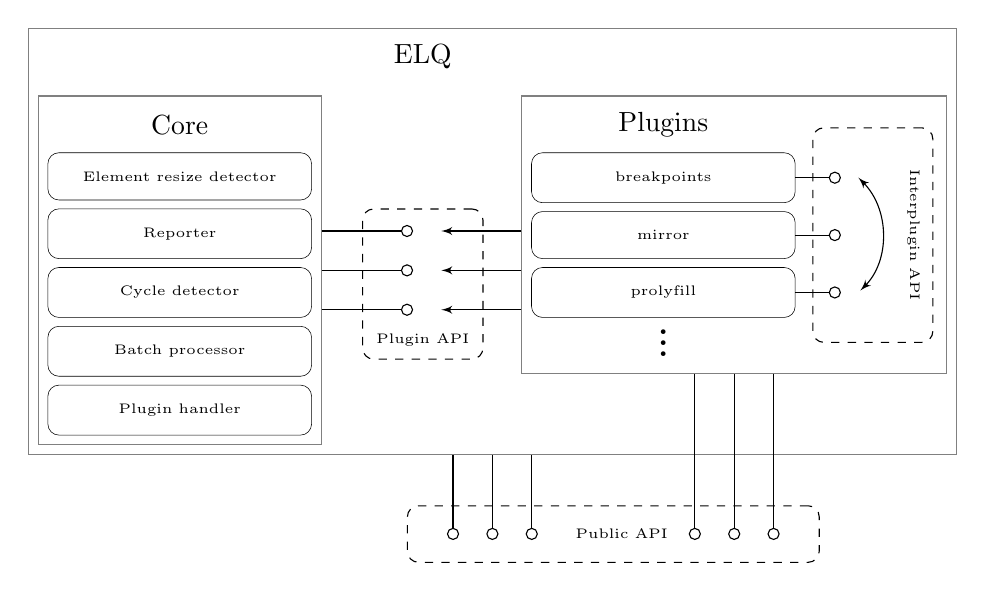
\begin{tikzpicture}[node distance=3pt]  
\tiny
  \tikzset{
      insidenode/.style={
        rectangle,
        rounded corners,
        draw=black,
        top color=white,
        bottom color=white,
        very thin,
        inner sep=1em,
        minimum height=2em,
        text centered,
        text width=12em
      },
      title/.style={
        draw=none,
        fill=none,
        top color=white,
        bottom color=white,
        thin,
        inner sep=0,
        minimum height=2em,
        text centered
      },
      box/.style={
        draw=black!50,
        inner sep=0.5em
      },
      o/.style={
        shorten >=#1,
        decoration={
          markings,
          mark={
            at position 1
            with {
              \draw circle [radius=#1];
            }
          }
        },
        postaction=decorate
      },
      o/.default=2pt,
      apibox/.style={
        minimum height=3em,
        dashed,
        draw=black,
        rounded corners
      },
      myarrow/.style={->, >=latex', shorten >=1pt, thin},
      mylabel/.style={text width=3em, text centered}
  }

  \node[] (middledummy) {};
  \node[title, above=15pt of middledummy] (elqtitle) {\normalsize ELQ};

  \node[title, left=11em of middledummy] (coretitle) { \normalsize Core };
  \node[insidenode, below=of coretitle] (erd) {Element resize detector};  
  \node[insidenode, below=of erd] (reporter) {Reporter};
  \node[insidenode, below=of reporter] (cycle) {Cycle detector};
  \node[insidenode, below=of cycle] (batch) {Batch processor};
  \node[insidenode, below=of batch] (plugin) {Plugin handler};

  \node[box, fit={(coretitle) (erd) (reporter) (cycle) (batch) (plugin)}] (core) {};

  \node[title, right=10em of middledummy] (pluginstitle) { \normalsize Plugins };
  \node[insidenode, below=of pluginstitle] (breakpoints) {breakpoints};
  \node[insidenode, below=of breakpoints] (mirror) {mirror};
  \node[insidenode, below=of mirror] (prolyfill) {prolyfill};
  \node[below=-4pt of prolyfill] (dots) {\huge \vdots};
  \node[box, fit={(pluginstitle) (breakpoints) (mirror) (prolyfill) (dots) ($ (breakpoints.east) + (1.8,0) $)}] (plugins) {};

  \node[box, fit={(elqtitle) (core) (plugins)}] (elq) {};

  % Interplugin API
  \draw[o] (breakpoints.east) -- ($ (breakpoints.east) + (0.5,0) $);
  \draw[o] (mirror.east) -- ($ (mirror.east) + (0.5,0) $);
  \draw[o] (prolyfill.east) -- ($ (prolyfill.east) + (0.5,0) $);
  \draw[myarrow, <->] ($ (breakpoints.east) + (0.8,0) $) to[out=-45, in=45] ($ (prolyfill.east) + (0.8,0) $);
  \node[mylabel, rotate=-90, text width=10em] (interpluginapilabel) at ($ (mirror.east) + (1.5,0) $) {Interplugin \gls{API}};
  \node[apibox, fit={($ (breakpoints.east) + (0.3,0.5) $) ($ (prolyfill.east) + (0.3,-0.5) $) (interpluginapilabel)}] (interpluginapi) {};

  % Public API
  \coordinate (pubapibottom) at ($ (elq.south) + (0,-1) $);
  \draw[o] ($ (elq.south) + (0,0) $) -| (pubapibottom);
  \draw[o] ($ (elq.south) + (-0.5,0) $) -| ($ (pubapibottom) + (-0.5,0) $);
  \draw[o] ($ (elq.south) + (0.5,0) $) -| ($ (pubapibottom) + (0.5,0) $);
  \draw[o] let \p1=(pubapibottom), \p2=(plugins.south) in ($ (plugins.south) + (0,0) $) -| ($ (\x2,\y1) + (0,0) $);
  \draw[o] let \p1=(pubapibottom), \p2=(plugins.south) in ($ (plugins.south) + (0.5,0) $) -| ($ (\x2,\y1) + (0.5,0) $);
  \draw[o] let \p1=(pubapibottom), \p2=(plugins.south) in ($ (plugins.south) + (-0.5,0) $) -| ($ (\x2,\y1) + (-0.5,0) $);
  \node[mylabel, right=4em of pubapibottom, text width=5em] (pubapilabel) {Public \gls{API}};
  \path let \p1=(pubapibottom), \p2=(plugins.south) in node (pubapiright) at ($ (\x2,\y1) + (0.5,0) $) {};
  \node (pubapileft) at ($ (pubapibottom) + (-0.5,0) $) {};
  \node[apibox, fit={(pubapibottom) (pubapilabel) ($ (pubapileft) + (-0.5,0) $) ($ (pubapiright) + (0.5,0) $)}] (publicapi) {};

  % Plugin API
  \path let \p1=(middledummy.south), \p2=(core.east) in coordinate (pluginapi) at (\x1, \y2);
  \node[mylabel, below=3em of pluginapi, text width=5em] (pluginapilabel) {Plugin \gls{API}};
  \draw[o] ($ (core.east) + (0,0) $) -- ($ (pluginapi) + (-0.2,0) $);
  \draw[o] ($ (core.east) + (0,0.5) $) -- ($ (pluginapi) + (-0.2,0.5) $);
  \draw[o] ($ (core.east) + (0,-0.5) $) -- ($ (pluginapi) + (-0.2,-0.5) $);
  \draw[myarrow] let \p1=(core.east), \p2=(plugins.west) in ($ (\x2, \y1) + (0,0) $) -- ($ (pluginapi) + (0.2,0) $);
  \draw[myarrow] let \p1=(core.east), \p2=(plugins.west) in ($ (\x2, \y1) + (0,0.5) $) -- ($ (pluginapi) + (0.2,0.5) $);
  \draw[myarrow] let \p1=(core.east), \p2=(plugins.west) in ($ (\x2, \y1) + (0,-0.5) $) -- ($ (pluginapi) + (0.2,-0.5) $);
  \node[apibox, fit={(pluginapilabel) ($(pluginapi) + (0, 0.7)$)}] (pluginapibox) {};
\end{tikzpicture}
\medskip
\caption{
  The overall library architecture, which shows how the library is divided into two parts; the core and plugins. 
  The core is generally only accesible through the plugin \gls{API}, and is not a part of the public \gls{API}.
  Plugins may have interplugin \glspl{API} and dependencies.
  The bigger part of the public \gls{API} is defined by the plugins.
}
\label{fig:elq_architecture}
\end{figure}
      \todo{Change picture so that batch processor comes before the erd system}

      Figure~\ref{fig:elq_architecture} shows the overall architecture of the library.
      The core consists of fundamental and general subsystems that are utilized by plugins.
      Developers should generally never be programming against the core directly, and it can therefore only be accessed by plugins through a hidden plugin \gls{API} (with the exception of few core methods that are part of the public \gls{API}).
      The role of the library is to provide plugins with subsystems to be used for performing element query tasks, which is done through the plugin \gls{API}.
      \todo{Does this sentence fit here?}
      The library provides a small public \gls{API} that is mainly used to handle and invoke plugins.
      The plugins form the bigger part of the public \gls{API} in the sense that they decide the features that exist and how they work.
      It should be noted that plugins might provide \glspl{API} through the library by registering methods, or by specifying custom syntax (such as markup or \gls{CSS}), which is beyond the control of the core.
      \todo{It is right now not possible to register methods on ELQ. Maybe it should be.}
      Plugins may also have interplugin \glspl{API} and dependencies, which also is beyond the control of the core.
      The core is supposed to have a slow development rate, with few breaking changes to provide good backward compatibility.
      Plugins may be developed in a high rate, with frequent changes to support new features.
      Subsystems that are part of the core are the following:
      \begin{itemize}
        \item \textbf{Reporter:}
          Responsible for reporting information, warnings and errors to the developer.
          By having a centralized reporter, it is possible to decide at a global library level how much plugins are allowed to report.
          Other options such as throwing exception on errors or warnings could also be set at a global library level.
          Also, the library can make sure that all reports are standardized and can provide extra information such as the name and version of the plugin along with its report.
          To avoid code duplication, it also beneficial to have a centralized reporting system so plugins do not need to perform the same compatibility checks (such as checking if the \gls{browser} actually supports console reporting).
        \item \textbf{Batch processor:}
          To avoid \gls{layout thrashing} as described in Section~\ref{sec:layout-thrashing}, it is important to read and mutate the \gls{DOM} in separate \glslink{batch processing}{batches}.
          This subsystem provides an interface for plugins to store functions to later be executed in \glslink{batch processing}{batches}.
          It supports executing \glslink{batch processing}{batches} asynchronously and also provides an interface for dividing \glslink{batch processing}{batches} up in levels that are executed in order.
          This subsystem is described further in Section~\ref{sec:imp_batch_processor}.
        \item \textbf{Element resize detector:}
          Provides an interface for observing \gls{element} resize events, which is fundamental to plugins fulfilling requirements \ref{itm:req_resize_detect} and \ref{itm:req_big_rewrite}.
          It enables the library to observe \glspl{element} resize events, instead of the application keeping track of when \glspl{element} are resized.
          This subsystem is described further in Section~\ref{sec:imp_erd}.
          \todo[inline]{Maybe this shouldn't be a core subsystem? Since this system imposes the biggest performance impact. It might make more sense to have this as a plugin.}
        \item \textbf{Cycle detector:}
          Responsible for detecting cycles and warning about them.
          As shown in Section~\ref{sec:cyclic-rules} cyclic rules need to be detected at runtime.
          When a plugin wish to update the size state of an \gls{element} (which in turn applies the conditional styles) it can ask this system if the update seems to be part of a cycle.
          If the update seems to be part of a cycle, it is up to the plugin how that should be handled.
          This subsystem is described further in Section~\ref{sec:imp_cycle_detector}.
          \todo[inline]{Write that this system is more general, and could potentially be used for detecting other cyclic behaviors?}
        \item \textbf{Plugin handler:}
          Of course, having plugins requires a subsystem for handling them.
          This system provides an interface for developers to register plugins to the library.
          The system is also responsible for retrieving the plugins, and invoking them on different library events.
      \end{itemize}
      Some of the subsystems may be partially accessible through the public \gls{API} such as the plugin handler and the \gls{element} resize detector.
      It should be noted that some subsystems have been intentionally left out due to being too small or insignificant to understand the overall architecture of the library.

   
    %%%%%%%%%%%%%%%%%%%%%%%%%%%%%%%%%%%%%%%%%%%%%%%%%%%%%%%%%%%%%%%%%%%%%%%%%%%%%%%%%%%%%%%%%%%%%%%%%%%%%%%%%%%%%%%%%%%%%%%%%%%%%%%%%%%%%%%%%%%%%%%%%%%%%%%%%%%%%%%%%%%%%%%%%%%%%%%%%%%%%%%%%%%%%%%%%%%%%%%%%%%%%%%%%%%%%%%%%%%%%%%%%%%%%%%%%%%%%%%%%%%%%%%%%%%%%%%%%%%%%%%%%%%%%%%%%%%%%%%%%%%%%%%%%%%%%%%%%%%%%%%%%%%%%%%%%%%%%%%%%%%%%%%%%%%%%%%%%%%%%%%%%%%%%%%%%%%%%%%%%%
    %%%%%%%%%%%%%%%%%%%%%%%%%%%% API design
    %%%%%%%%%%%%%%%%%%%%%%%%%%%%%%%%%%%%%%%%%%%%%%%%%%%%%%%%%%%%%%%%%%%%%%%%%%%%%%%%%%%%%%%%%%%%%%%%%%%%%%%%%%%%%%%%%%%%%%%%%%%%%%%%%%%%%%%%%%%%%%%%%%%%%%%%%%%%%%%%%%%%%%%%%%%%%%%%%%%%%%%%%%%%%%%%%%%%%%%%%%%%%%%%%%%%%%%%%%%%%%%%%%%%%%%%%%%%%%%%%%%%%%%%%%%%%%%%%%%%%%%%%%%%%%%%%%%%%%%%%%%%%%%%%%%%%%%%%%%%%%%%%%%%%%%%%%%%%%%%%%%%%%%%%%%%%%%%%%%%%%%%%%%%%%%%%%%%%%%%%%
    \section{API design}\label{sec:elq-api}
      \subsection{Public API}\label{sec:public-api}
        As already stated, the bigger part of the public \gls{API} is provided by plugins.
        In Section~\ref{sec:techincal-goals} it was determined that advanced users must be able to change the subsystems of the core.
        Therefore no global library instance is instantiated automatically on page load.
        Instead, a factory function \code{Elq} that creates \gls{ELQ} instances is provided in order to be able to inject dependencies.
        The function accepts an optional options object parameter, where it is possible to set options and subsystems to be used for the created instance.
        If no options are given, default options will be used.
        See listing~\ref{code:elq-ctor} of example usages of the \code{Elq} function.
        The function returns an object containing the core public \gls{API} methods of the \gls{ELQ} instance.
        \todo{Write about bare builds, so that the unused default subsystems are not being loaded?}
        \begin{lstlisting}[gobble=10,caption={Example usages of the \code{Elq} factory function that creates \gls{ELQ} instances.},captionpos=b,label={code:elq-ctor}]]
          //Default options being used.
          var elq = Elq();

          //A custom reporter and cycle detector being used.
          var customCycleDetector = ...;
          var customReporter = ...;
          var elq2 = Elq({
            reporter: customReporter,
            cycleDetector: customCycleDetector
          });
        \end{lstlisting}

        The next step after creating an instance is to register the plugins to be used by the instance.
        There are two methods for handling plugins: \code{use} and \code{using}.
        The \code{use} method registers a plugin to be used by the library instance.
        It is responsible for controlling that plugins do not conflict with each other and that plugins are initiated correctly with the plugin \gls{API} of the library instance.
        The method requires a \emph{plugin definition object} (or shortened \emph{plugin definition}) parameter, and also accepts an optional options object parameter.
        A plugin definition is responsible for describing a plugin and providing a factory function \code{make} that creates a plugin instance.
        The function requires an \code{elq} parameter that is the \gls{ELQ} instance extended with the plugin \gls{API}, and accepts an optional \code{options} object parameter.
        Plugin definitions also expose methods that are called by \gls{ELQ} in order to retrieve the name, version and compatibility of a plugin.
        When \code{use} is called, it creates a plugin instance by invoking the \code{make} factory function (with the \code{use} options parameter as argument to \code{make}) and returns the created instance so that the user may store the reference to the plugin instance.
        The \code{using} method requires a \emph{plugin identifier} parameter and tells if the given plugin is being used (i.e., has been registered) by the instance or not.
        The plugin identifier of a plugin is either the plugin definition or the name of the plugin.
        See listing~\ref{code:plugin-object} for an example plugin definition and how it is used with the two methods for handling plugins.

        \begin{lstlisting}[gobble=10,caption={Example plugin definition and examples of handling plugins.},captionpos=b,label={code:plugin-object}]]
          // An example plugin definition.
          var myPlugin = {
            getName: function() {
              // Returns the name of the plugin, which has to be 
              // unique in an elq instance.
              return "my-plugin";
            },
            getVersion: function() {
              // Returns the version of the plugin.
              return "1.0.0";
            },
            isCompatible: function(elq) {
              // Returns a boolean that indicates if this plugin
              // is compatible with the given elq instance.
              return true;
            },
            make: function(elq, options) {
              // The elq parameter is the plugin API of the ELQ instance,
              // and is not the same object returned by the Elq factory function.

              // Returns a plugin instance. It is optional to use
              // the elq instance or options object in the initiation process.
              return {...};
            }
          };

          // Tell the elq instance to use myPlugin with default options.
          var myPluginInstance1 = elq.use(myPlugin);

          // Tell the elq2 instance to use myPlugin with custom options.
          var options = {...};
          var myPluginInstance2 = elq2.use(myPlugin, options);

          // The plugin instances are not equal since they 
          // have been initated to different elq instances.
          myPluginInstance1 !== myPluginInstance2 // true

          // Check if the plugin is being used.
          elq.using(myPlugin); // true

          // Also possible to check by the plugin name.
          elq.using("my-plugin"); // true

          // Plugins not being used by the instance returns false.
          elq.using("other-plugin"); // false
        \end{lstlisting}

        When the desired plugins have been registered to the \gls{ELQ} instance, it is time to initialize the library to the target \glspl{element}.
        This is done with the \code{start} method that requires a collection of \glspl{element} as a parameter.
        When called, it will invoke all \code{start} methods on all registered plugins that gives them the opportunity to initiate the \glspl{element} according to their own mechanisms.
        To satisfy the requirements \ref{itm:natural} and \ref{itm:assumption} the function is agnostic about the \glspl{element} collection --- all objects that are iterable and contains \glspl{element} are accepted.
        It is also possible to provide a single \gls{element} without a collection.
        The effect of calling the \code{start} method on an element multiple times is defined by the plugins.
        \todo{Rename start?}
        See listing~\ref{code:elq-start} for example usages of the \code{start} method.
        \begin{lstlisting}[gobble=10,caption={Example usages of the \code{start} method. The method only requires an iterable collection, so it is library agnostic.},captionpos=b,label={code:elq-start}]]
          // Initiating the library to a single element.
          var singleElement = document.getElementById("...");
          elq.start(singleElement);

          // Initiating the library to multiple elements.
          var singleElement2 = document.getElementById("...");
          elq.start([singleElement, singleElement2]);

          // Initiating the library to multiple elements using
          // third-party libraries (in this case jQuery).
          var jqueryElementsCollection = $("...");
          elq.start(jqueryElementsCollection);

          // Native API's are also supported.
          var nativeElementsCollection = document.querySelectorAll("...");
          elq.start(nativeElementsCollection);
        \end{lstlisting}

        \todo[inline]{The current elq.use syntax disallows chaining. Should think about how to register multiple plugins at the same time.}
        \todo[inline]{Describe the listenTo method?}

      \subsection{Plugin API}\label{sec:plugin-api}
        The plugin \gls{API} is a superset of the public \gls{API}.
        Plugins have additional direct access to most core subsystems presented in Section~\ref{sec:arcithecture}.
        Recall that access to the plugin \gls{API} is given to a plugin when it is registered (i.e., when the \gls{ELQ} instance invokes the \code{make} function of the plugin definition).
        Since the plugin handler and element resize detector subsystems are exposed through to public \glspl{API} they cannot be directly accessed through the plugin \gls{API}.
        However, an additional method \code{getPlugin} of the plugin handler system is exposed that returns the registered plugin instance given a plugin identifier parameter.
        This method is facilitates interplugin communications.
        Direct access is given to the following core subsystems:
        \begin{itemize}
          \item 
            \textbf{Reporter}: via the \code{elq.reporter} property that refers to the reporter instance.
            The reporter has three methods: \code{log}, \code{warn} and \code{error} that are used to report information, warnings and errors respectively.
            The default behavior of the reporter is to report to the \gls{browser} console\footnote{See \url{https://developer.mozilla.org/en-US/docs/Web/API/Console} for more information.} if possible.
          \item
            \textbf{Cycle detector}: via the \code{elq.cycleDetector} property that refers to the cycle detector instance.
            The cycle detector has a method \code{isUpdateCyclic} that tells if the desired state update of an element seems to be part of a cycle.
            To do so, it requires two parameters; the target \gls{element} and the state update itself.
            A third update time parameter, which defines when the update was requested, is optional and will default to the time of the method call.
          \item 
            \textbf{Batch processor}: via the \code{elq.BatchProcessor} property that refers to a factory function that creates \glslink{batch processing}{batch processor} instances.
            Instead of having a single \glslink{batch processing}{batch processor} instance shared among all library entities (i.e., core subsystems and plugins), each entity has to create an own instance.
            This to avoid entities interfering with each other while processing \glslink{batch processing}{batches}.
            For example, some entities might want to force the \glslink{batch processing}{batch} to be processed at a point where it would be beneficial for other entities to delay the processing.
            The \code{createBatchProcessor} accepts an optional options object parameter and returns a \glslink{batch processing}{batch processor} instance
            Two important options to the \code{createBatchProcessor} are the \code{async} and \code{auto} options.
            If the \code{async} option is enabled, the \glslink{batch processing}{batch} will be processed asynchronously as soon as possible after that the \code{force} method has been invoked.
            If the \code{auto} option is enabled, the \glslink{batch processing}{batch} will automatically be processed as soon as possible asynchronously (this implies that \code{async} has to be enabled).
            The \glslink{batch processing}{batch processor} instance has two methods: \code{add} and \code{force}.
            The \code{add} method requires a function parameter that will be called when the \glslink{batch processing}{batch} is processed, and accepts an optional level parameter that defines at which level the given function should be processed.
            The \code{force} method commences the processing of the \glslink{batch processing}{batch}, which can happen synchronously or asynchronously defined by an optional parameter.
            \todo{Move some of this text to the own batch processor section in implementation details.}
          \item
            \textbf{\abbr{ID} handler}: via the \code{elq.idHandler} property that refers to the \abbr{ID} handler instance. \todo{Include id handler in section \ref{sec:arcithecture}?}
            The \abbr{ID} handler has a method \code{get} that returns the \abbr{ID} of the required element parameter.
            If the element does not have any \abbr{ID} one will be assigned to the \gls{element}.
            It is possible to override the assignment with an option parameter.
        \end{itemize}
      \subsection{Plugins}
        Now, it is time to describe the systems and \glspl{API} that actually realizes element queries as \gls{ELQ} plugins.
        The plugins presented here is the suggested solution to element queries according to the research of this thesis.
        They are designed for adequate performance, good compatibility, and ease of use.
        For extreme requirements or corner cases, custom \gls{ELQ} plugins might be preferred.
        It should be noted that the development of the prolyfill plugin is left for future work.

        \Gls{ELQ} plugins may use custom element attributes as part of their \glspl{API}.
        The \gls{HTML} standard supports custom attributes prefixed with \code{data-}.
        Modern \glspl{browser} usually permit to discard the \code{data-} prefix for custom attributes.
        For visual reasons, custom attributes will be written in the shortest possible way in this thesis (without the \code{data-} prefix).
        Although not written in the examples the library and all plugins support both ways of defining custom \gls{element} attributes, so it is able to conform to the \gls{HTML} standard.
        \todo[inline]{Need to implement this in ELQ.}
        \todo[inline]{Maybe it should be generally explained that the attribute design of both plugins follow the same design. Explain options at element level, plugin level, etc.}

        \subsubsection{Breakpoints}\label{sec:plugin-breakpoints}
          This plugin observes element resize events and updates the \glspl{element} size states according to defined breakpoints.
          The name of the plugin is \code{elq-breakpoints} and it does not have any dependencies (other than the element resize detector of the \gls{ELQ} core).
          The main idea of the plugin is to apply classes to target \glspl{element} that reflect the size states of the \glspl{element}.
          Style states of an element are defined by breakpoints by custom element attributes.
          See listing~\ref{code:elq-breakpoints-example} for an example of breakpoints definition attributes.
          \begin{lstlisting}[gobble=12,caption={Example of an element that has two width breakpoints (300 and 500 pixels) defined by using the \code{elq-breakpoints} plugin.},captionpos=b,label={code:elq-breakpoints-example}]]
            <div id="target" elq elq-breakpoints elq-breakpoints-width="300 500">
            ...
            </div>
          \end{lstlisting}
          \todo{Shorten syntax?}
          The \code{elq} attribute states that it is an \gls{ELQ} \gls{element}, and the \code{elq-breakpoints} attribute states that the \gls{element} should be handled by the plugin.
          The \code{elq-breakpoints\-width="300 500"} defines that the \gls{element} should have width breakpoints at 300 and 500 pixels.
          Height breakpoints are defined in the same way with the \code{elq-breakpoints-height} attribute.
          The possible size states of the \gls{element} would then be (in pixels):
          \begin{itemize}
            \item $width < 300$
            \item $300 <= width < 500$
            \item $500 <= width$
          \end{itemize}
          \todo{Explain that low is inclusive, and why.}
          The plugin appends classes to the \gls{element} that reflects the size state of the \gls{element}.
          For each breakpoint, one class is present that tells if the size is above or below the breakpoint.
          \todo{Remember that above is inclusive. Maybe this should be an option?}
          Recall from Section~\ref{sec:eq-definitions} that the number of size states of an \gls{element} in a dimension is given by $n_{ss}(n_b) = n_b + 1$, where $n_b$ is the number of breakpoints in that dimension.
          Since the style state can be either above or below each breakpoint, the number of breakpoint classes of an \gls{element} in a dimension is given by $n_{bc}(n_{b}) = 2n_b$.
          The number of breakpoint classes active at the same time for an \gls{element} in a dimension is given by $n_{abc}(n_{b}) = n_{b}$.
          The format of the classes is: \\*\code{elq-[width|height]-[above|below]-[breakpoint][postfix]}.
          \todo{Format this better.}
          It is possible to define a postfix to be applied to all breakpoint classes by the \code{postfix} option either at \gls{element} level (i.e., by adding \code{postfix} as the attribute value of \code{elq-breakpoints}) or as a plugin instance option when registering the plugin with the \code{use} method of \gls{ELQ}.
          For example, if the width of the \gls{element} described in listing~\ref{code:elq-breakpoints-example} is narrower than 300 pixels, it will have the following two classes present:
          \begin{itemize}
            \item \code{elq-width-below-300}
            \item \code{elq-width-below-500}
          \end{itemize}
          \todo{Motivate this design.}
          The breakpoint classes are used for applying conditional styles for \glspl{element} based on the size state of the target \gls{element}.
          See listing~\ref{code:elq-breakpoints-style} for an example of conditional styling the the \code{\#target} element and its children as presented in listing~\ref{code:elq-breakpoints-example}.
          \begin{lstlisting}[gobble=12,caption={Example of conditional styles using the \code{elq-breakpoints} plugin classes.},captionpos=b,label={code:elq-breakpoints-style}]]
            #target {
              color: black;
              font-size: 15px;
            }

            #target.elq-width-below-300   { font-size: 10px;  }
            #target.elq-width-above-300   { color: red;       }
            #target.elq-width-above-500   { font-size: 20px;  }
            #target.elq-width-above-500 p { padding: 10px;    }
            #target.elq-width-below-500 p { padding: 5px;     }
          \end{lstlisting}
          In this example it is shown that an element can be conditionally styled by their own size.
          Additionally, children can be conditionally styled by adding the child simple selector to the right of the simple selector containing the element breakpoint classes.
          For instance, in the example all paragraph \glspl{element} \code{p} will be styled conditionally by the target element size state.

          \todo[inline]{Example of how to register the plugin with an elq instance + options?}
          \todo[inline]{Write that above is inclusive and below is exclusive? Why? Option?}
          \todo[inline]{Write about the interplugin API methods that mirror uses?}
          \todo[inline]{Write about noclasses option and the use case for it.}
          \todo[inline]{If postfix=px maybe it should be supported to write elq-breakpoints-width="500px 700px" etc.}
        \subsubsection{Mirror}\label{sec:plugin-mirror}
          % As of the \gls{CSS3} specification, there is no way to select ancestor elements of an element.
          % For instance, \code{p img} is a selector that matches all image elements that are contained by a paragraph.
          % However, it is not possible to construct a selector that matches all paragraphs that contains images.

          This plugin complements the \code{elq-breakpoints} plugin and is needed in some cases due to limitations of CSS.
          Suppose that it is desired for an application to style all paragraph \glspl{element} differently by the size of the nearest element with a \code{container} class.
          Paragraphs may appear nested in other \glspl{element}, which may be generated dynamically at runtime.
          Therefore, the structure of the application is not known when writing the \gls{CSS}, so no assumptions can be done about the markup structure.
          Consider the example markup given in listing~\ref{code:elq-mirror-example} for an example \gls{HTML} structure.
          It should be noted that the \code{container} \glspl{element} might be styled in any way (e.g., the widths of the inner container \gls{element} could be relative to the outer container \gls{element}).
          \begin{lstlisting}[gobble=12,caption={Example \gls{HTML} structure where all paragraphs are desired to be conditionally styled by the nearest ancestor container.},captionpos=b,label={code:elq-mirror-example}]
            <div class="container" elq elq-breakpoints elq-breakpoints-width="300 500">
              <div>
                <p>Paragraph 1</p>
              </div>

              <div class="container" elq elq-breakpoints elq-breakpoints-width="300 500">
                <p>Paragraph 2</p>
              </div>
              <div class="container" elq elq-breakpoints elq-breakpoints-width="300 500">
                <p>Paragraph 3</p>
              </div>
            </div>
          \end{lstlisting}
          A naive approach to conditionally style the paragraph \glspl{element} is using the selector structure given in listing~\ref{code:elq-mirror-example-cont}.
          \begin{lstlisting}[gobble=12,caption={A naive approach to conditionally style the paragraph \glspl{element} by the size of the nearest ancestor container \gls{element}.},captionpos=b,label={code:elq-mirror-example-cont}]
            .container p                      { background-color: red;    }
            .container.elq-width-above-300 p  { background-color: yellow; }
            .container.elq-width-above-500 p  { background-color: green;  }
          \end{lstlisting}
          The problem with this is that the selectors state that all paragraphs that are children of \emph{any} container should be styled in some way.
          So if the outer container element is 600 pixels wide and the inner containers are 200 pixels wide, all paragraphs would be colored green because they have an ancestor container that is wider than 500 pixels (i.e., the outer container).
          The desired behavior is that the first paragraph is colored green and the two inner paragraphs colored red, since the widths of the inner containers are narrower than 300 pixels.
          As of the \gls{CSS} selectors level 3 specification, there it is not possible to select the nearest ancestor of an element \cite{w3c_css_selectors}.
          
          The \code{elq-mirror} plugin overcome these limitations by mirroring the breakpoint classes of an \code{elq-breakpoints} element and thus the correct behavior can be achieved.
          \Glspl{element} are initialized to mirror such \glspl{element} by adding attributes in the same way like with the \code{elq-breakpoints} plugin.
          The mirror \glspl{element} will then match the breakpoint classes of the nearest ancestor that has the \code{elq-breakpoints} attribute.
          See listing~\ref{code:elq-mirror-example-cont-2} for how the plugin can be used to achieve the desired behavior of the conditionally styled paragraphs.
          % If no such ancestor is found, the document root will be mirrored instead. //TODO: Have this?
          \begin{lstlisting}[gobble=12,caption={By using the \code{elq-mirror} plugin to overcome the limitations of CSS, the correct behavior can be achieved of the conditionally styled paragraphs.},captionpos=b,label={code:elq-mirror-example-cont-2}]
            /* HTML */
            <div class="container" elq elq-breakpoints elq-breakpoints-width="300 500">
              <div>
                <p elq elq-mirror>Paragraph 1</p>
              </div>

              <div class="container" elq elq-breakpoints elq-breakpoints-width="300 500">
                <p elq elq-mirror>Paragraph 2</p>
              </div>
              <div class="container" elq elq-breakpoints elq-breakpoints-width="300 500">
                <p elq elq-mirror>Paragraph 3</p>
              </div>
            </div>

            /* CSS */
            .container p                      { background-color: red;    }
            .container p.elq-width-above-300  { background-color: yellow; }
            .container p.elq-width-above-500  { background-color: green;  }
          \end{lstlisting}
          Notice that the breakpoint classes now are used in conjunction with the paragraph simple selector instead of the container in the CSS selectors.
          This way, the conditional styles behave as expected since all paragraphs are by the nearest (instead of any) container \gls{element}.

          By mirroring element breakpoint classes, \glspl{element} can be styled by criteria of any element (ancestor, sibling, child, etc.).
          The plugin is at the moment restricted to the nearest ancestor \code{elq-breakpoint} \gls{element}, but could easily be extended to support more advanced mirror constellations.
    %%%%%%%%%%%%%%%%%%%%%%%%%%%%%%%%%%%%%%%%%%%%%%%%%%%%%%%%%%%%%%%%%%%%%%%%%%%%%%%%%%%%%%%%%%%%%%%%%%%%%%%%%%%%%%%%%%%%%%%%%%%%%%%%%%%%%%%%%%%%%%%%%%%%%%%%%%%%%%%%%%%%%%%%%%%%%%%%%%%%%%%%%%%%%%%%%%%%%%%%%%%%%%%%%%%%%%%%%%%%%%%%%%%%%%%%%%%%%%%%%%%%%%%%%%%%%%%%%%%%%%%%%%%%%%%%%%%%%%%%%%%%%%%%%%%%%%%%%%%%%%%%%%%%%%%%%%%%%%%%%%%%%%%%%%%%%%%%%%%%%%%%%%%%%%%%%%%%%%%%%%
    %%%%%%%%%%%%%%%%%%%%%%%%%%%% Implementation
    %%%%%%%%%%%%%%%%%%%%%%%%%%%%%%%%%%%%%%%%%%%%%%%%%%%%%%%%%%%%%%%%%%%%%%%%%%%%%%%%%%%%%%%%%%%%%%%%%%%%%%%%%%%%%%%%%%%%%%%%%%%%%%%%%%%%%%%%%%%%%%%%%%%%%%%%%%%%%%%%%%%%%%%%%%%%%%%%%%%%%%%%%%%%%%%%%%%%%%%%%%%%%%%%%%%%%%%%%%%%%%%%%%%%%%%%%%%%%%%%%%%%%%%%%%%%%%%%%%%%%%%%%%%%%%%%%%%%%%%%%%%%%%%%%%%%%%%%%%%%%%%%%%%%%%%%%%%%%%%%%%%%%%%%%%%%%%%%%%%%%%%%%%%%%%%%%%%%%%%%%%
    \section{Details of subsystems}\label{sec:library-imp-details}
      In this Section the algorithms and approaches of some subsystems are presented.
      It should be noted that only the non-trivial subsystems are described.

      %%%%%%%%%%%%%%%%%%%%%%%%%%%%%%%%%%%%%%%%%%%%%%%%%%%%%%%%%%%%%%%%%%%%%%%%%%%%%%%%%%%%%%%%%%%%%%%%%%%%%%%%%%%%%%%%%%%%%%%%%%%%%%%%%%%%%%%%%%%%%%%%%%%%%%%%%%%%%%%%%%%%%%%%%%%%%%%%%%%%%%%%%%%%%%%%%%%%%%%%%%%%%%%%%%%%%%%%%%%%%%%%%%%%%%%%%%%%%%%%%%%%%%%%%%%%%%%%%%%%%%%%%%%%%%%%%%%%%%%%%%%%%%%%%%%%%%%%%%%%%%%%%%%%%%%%%%%%%%%%%%%%%%%%%%%%%%%%%%%%%%%%%%%%%%%%%%%%%%%%%%
      %%%%%%%%%%%%%%%%%%%%%%%%%%%% Batch processor
      %%%%%%%%%%%%%%%%%%%%%%%%%%%%%%%%%%%%%%%%%%%%%%%%%%%%%%%%%%%%%%%%%%%%%%%%%%%%%%%%%%%%%%%%%%%%%%%%%%%%%%%%%%%%%%%%%%%%%%%%%%%%%%%%%%%%%%%%%%%%%%%%%%%%%%%%%%%%%%%%%%%%%%%%%%%%%%%%%%%%%%%%%%%%%%%%%%%%%%%%%%%%%%%%%%%%%%%%%%%%%%%%%%%%%%%%%%%%%%%%%%%%%%%%%%%%%%%%%%%%%%%%%%%%%%%%%%%%%%%%%%%%%%%%%%%%%%%%%%%%%%%%%%%%%%%%%%%%%%%%%%%%%%%%%%%%%%%%%%%%%%%%%%%%%%%%%%%%%%%%%%
      \subsection{Batch processor}\label{sec:imp_batch_processor}
        % To avoid \gls{layout thrashing} by other scripts it can beneficial to asynchronously postpone the \glslink{batch processing}{batch} until the next layout cycle of the \gls{browser}, which is also handled by the subsystem.
        Both Section~\ref{sec:layout-process} and \ref{sec:layout-thrashing} is recommended to read in order to understand the optimizations described in this section.
        The \glslink{batch processing}{batch processor} is the foundation for good performance of the library, and is therefore used by several subsystems.
        It serves two purposes:
        \begin{enumerate}
          \item Automatically process a \glslink{batch processing}{batch} asynchronously.
          \item Process a \glslink{batch processing}{batch} in different levels.
        \end{enumerate}
        
        \paragraph{Automated processing}
        The automated asynchronous processing of \glslink{batch processing}{batches} is important because some subsystems do not know how many operations are to be performed when invoked.
        For instance, the public \gls{ELQ} \gls{API} method \code{start} is called with \glspl{element} to be initiated by the library.
        As part of the initialization, the element resize detection subsystem may be invoked so it can prepare \glspl{element} to be detectable.
        This needs to be \glslink{batch processing}{batch} processed, which is possible to do synchronously.
        However, if the \code{start} method is called multiple times synchronously \gls{layout thrashing} occurs since one \glslink{batch processing}{batch} for each method call is created.
        See listing~\ref{code:batch-processor-example} for example code that invokes the \code{start} method multiple times synchronously.
        \begin{lstlisting}[gobble=10,label={code:batch-processor-example},caption={Example of multiple synchronous calls to the \gls{ELQ} \code{start} method.},captionpos=b]]
          elq.start(document.getElementById("..."));
          elq.start(document.getElementById("..."));
          elq.start(document.getElementById("..."));

          var elements = [...];
          elements.forEach(elq.start);
        \end{lstlisting}
        Of course, such usage could be warned against in the \gls{API} documentation but to keep the \gls{API} as simple as possible another approach has been taken.
        By delaying the \glslink{batch processing}{batch} to execute asynchronously all synchronous calls of the method is grouped into the pending \glslink{batch processing}{batch}.
        Since a single shared \glslink{batch processing}{batch} is used for all method calls \gls{layout thrashing} is avoided.
        
        This behavior can be controlled by the \code{async} and \code{auto} options of the \glslink{batch processing}{batch processor} factory function.
        If the \code{async} option is enabled, the \glslink{batch processing}{batch} is processed asynchronously as soon as possible after that the \code{force} method has been invoked.
        If the \code{auto} option is enabled, the \glslink{batch processing}{batch} is automatically processed as soon as possible asynchronously (this implies that \code{async} has to be enabled).

        \paragraph{Leveled processing}
        Being able to process a \glslink{batch processing}{batch} in levels is important when different types of operations, that are to be processed in a specific order (usually to avoid \gls{layout thrashing}), needs to be grouped together in a \glslink{batch processing}{batch}.
        For instance, a function that doubles an \gls{element}'s width and read the new calculated height benefits by being \glslink{batch processing}{batch} processed in three levels: reading the width, mutating the width, and reading the new height.
        Such function could also benefit from automatically process the \glslink{batch processing}{batch} so that the user may call the function multiple times synchronously.
        See listing~\ref{code:batch-processor-example-2} for an example implementation of such function that uses the leveled \glslink{batch processing}{batch processor}.
        The function achieves a 45-fold speedup when applied to 1000 \glspl{element} by processing the \glslink{batch processing}{batch} in levels compared to not doing so in Chrome version 43.
        \begin{lstlisting}[gobble=10,label={code:batch-processor-example-2},caption={Example function that doubles an \gls{element}'s width and returns the new height with a callback. The function uses the leveled \glslink{batch processing}{batch processor} to avoid \gls{layout thrashing} and thus gains a 45-fold speedup.},captionpos=b]]
          var batchProcessor = BatchProcessor({
              auto: true,
              async: true
            });

          function doubleWidth(element, callback) {
            var width = element.offsetWidth;
            var newWidth = (width * 2) + "px";

            // Implicit level 0 of the batch. Will be processed first.
            batchProcessor.add(function mutateWidth() {
              element.style.width = newWidth;
            });

            // Level 1 of the batch. Will be processed after level 0.
            // Changing the level number from "1" to "0" results in layout thrashing.
            batchProcessor.add(1, function readHeight() {
              var height = element.offsetHeight;
              callback(height);
            });
          }

          var elements = [...];
          elements.forEach(function (element) {
            doubleWidth(element, function (height) {
              ...
            });
          });
        \end{lstlisting}

      %%%%%%%%%%%%%%%%%%%%%%%%%%%%%%%%%%%%%%%%%%%%%%%%%%%%%%%%%%%%%%%%%%%%%%%%%%%%%%%%%%%%%%%%%%%%%%%%%%%%%%%%%%%%%%%%%%%%%%%%%%%%%%%%%%%%%%%%%%%%%%%%%%%%%%%%%%%%%%%%%%%%%%%%%%%%%%%%%%%%%%%%%%%%%%%%%%%%%%%%%%%%%%%%%%%%%%%%%%%%%%%%%%%%%%%%%%%%%%%%%%%%%%%%%%%%%%%%%%%%%%%%%%%%%%%%%%%%%%%%%%%%%%%%%%%%%%%%%%%%%%%%%%%%%%%%%%%%%%%%%%%%%%%%%%%%%%%%%%%%%%%%%%%%%%%%%%%%%%%%%%
      %%%%%%%%%%%%%%%%%%%%%%%%%%%% Element resize detection
      %%%%%%%%%%%%%%%%%%%%%%%%%%%%%%%%%%%%%%%%%%%%%%%%%%%%%%%%%%%%%%%%%%%%%%%%%%%%%%%%%%%%%%%%%%%%%%%%%%%%%%%%%%%%%%%%%%%%%%%%%%%%%%%%%%%%%%%%%%%%%%%%%%%%%%%%%%%%%%%%%%%%%%%%%%%%%%%%%%%%%%%%%%%%%%%%%%%%%%%%%%%%%%%%%%%%%%%%%%%%%%%%%%%%%%%%%%%%%%%%%%%%%%%%%%%%%%%%%%%%%%%%%%%%%%%%%%%%%%%%%%%%%%%%%%%%%%%%%%%%%%%%%%%%%%%%%%%%%%%%%%%%%%%%%%%%%%%%%%%%%%%%%%%%%%%%%%%%%%%%%%
      \subsection{Element resize detection}\label{sec:imp_erd}
        As described in Section~\ref{sec:arcithecture}, \gls{ELQ} needs a subsystem that is able to detect resize events of \glspl{element}.
        As the \gls{element} resize detection system is a core subsystem of \gls{ELQ}, and extensively used by the \code{elq-breakpoints} plugin, it is important to find a both stable and performant approach to detect \gls{element} resize events.

        Unfortunately, there is no standardized resize event for arbitrary \glspl{element} \cite{w3c_dom2_events}.
        Only \glspl{document} emit resize events in modern browsers and therefore such events can only be observed for frame \glspl{element} (since a frame \gls{element} has its own \gls{document}).
        Legacy versions of Internet Explorer (version 8 and down, but also some later versions depending on the quirks and \gls{document} mode\footnote{See \url{http://en.wikipedia.org/wiki/Quirks_mode} for more information about quirks mode.}) do support the resize event for arbitrary \glspl{element}.
        According to the general use case described in Section~\ref{sec:eq-definitions}, a valid limitation is to only support \gls{element} resize detection for non-void \glspl{element} (i.e., \glspl{element} that may contain content).
        This limitation is important since most approaches depend on injecting \glspl{element} into the target \gls{element}.
        It is a reasonable limitation since void \glspl{element} can easily be wrapped with non-void elements without affecting the page visually.
        Possible solutions to detect element resize events in modern \glspl{browser} are:
        \begin{enumerate}
          \item\label{itm:erd-approach-polling}
            \textbf{Polling-based solution}:
            To have a script running asynchronously checking \glspl{element} if they have resized.
            This can be achieved by using the \gls{JavaScript} \code{setInterval}\footnote{See \url{http://www.w3.org/html/wg/drafts/html/master/webappapis.html\#timers} for more information about \gls{JavaScript} timer functions.} function.
            Short polling intervals (high frequency) leads to being able to detect resize events quicker but having worse performance.
            Longer polling intervals (low frequency) leads to not being able to detect resize events as quickly but having better performance.
            The longest delay between an actual resize event and the detection is given by the polling interval time.
            This approach is the most robust, as it supports arbitrary \glspl{element} (including void \glspl{element}) and provides excellent \gls{browser} compatibility.
          \item\label{itm:erd-approach-object}
            \textbf{Object-based solution}:
            Since frame \glspl{element} are the only \glspl{element} that support resize events \glslink{native}{natively}, the idea is to inject a frame \gls{element} as a child to the target \gls{element} that is observed instead.
            It has been shown by \cite{backalley} that \code{object} is the most suitable frame \gls{element} to be used for this purpose as they have good \gls{browser} compatibility and adequate performance.
            The \code{object} is styled so that it always matches the size of the target \gls{element} and so that it does not affect the page visually.
            Then a resize event handler is attached to the \gls{document} of the \code{object} that emits a \code{resize} event\footnote{See \url{http://www.w3.org/TR/DOM-Level-3-Events/\#event-type-resize} for more information about the resize event.} for every target \gls{element} resize.
          \item\label{itm:erd-approach-scroll}
            \textbf{Scroll-based solution}:
            This solution injects an \gls{element} to the target element that contains multiple overflowing \glspl{element} that listens to \code{scroll} events\footnote{See \url{http://www.w3.org/TR/DOM-Level-3-Events/\#event-type-scroll} for more information about the \code{scroll} event.}.
            The overflowing \glspl{element} are styled so that \code{scroll} events are emitted when the target \gls{element} is resized.
            For detecting when the target \gls{element} shrinks, two \glspl{element} are needed; one for handling the scrollbars and one for causing them to scroll.
            Similarly, for detecting when the target \gls{element} expands, two \glspl{element} are needed in the same way.
            A container \gls{element} is injected that contains the four \glspl{element} and is styled so that it matches the size of the target \gls{element} and so that it does not affect the page visually.
          \item\label{itm:erd-approach-flow}
            \textbf{Flow-based solution}:
            This solution is similar to the scroll-based solution in the sense that it also injects \glspl{element} that have overflowing content.
            Instead of listening to \code{scroll} events, this solution uses flow events.
            The idea is to detect when scrollbars disappear (i.e., underflow of content since the target container has increased in size) and when scrollbars appear (i.e., overflow of content since the target container has decreased in size).
            Unfortunately such events are not standardized but \gls{Gecko}, \gls{WebKit} and \gls{Blink} support them (although by different \glspl{API})\footnote{See \url{https://developer.mozilla.org/en-US/docs/Web/Events/overflow} for more information about the \gls{Gecko} flow event \gls{API}.}.
            \gls{Blink} still supports the events but has deprecated them \cite{blink_deprecated_flow_events} since version 34.
        \end{enumerate}
        The polling-based solution is appealing because it does not mutate the \gls{DOM}, supports arbitrary \glspl{element}, and it provides excellent \gls{browser} compatibility since it does not rely on special \gls{element} behavior or similar.
        However, in order to prevent the \gls{responsive} \glspl{element} lagging behind the size changes of the user interface, polling needs to be performed quite frequently.
        Recall from Section~\ref{sec:layout-process} that \glspl{layout engine} typically have a layout queue in order to perform layout in \glslink{batch processing}{batches} for increased performance.
        Each poll would force the layout queue to be flushed since the computed style of \glspl{element} needs to be retrieved in order to know if \glspl{element} have resized or not.
        Since the polling is performed all the time the overall page performance is decreased even if the page is idle, which is undesired especially for devices running on battery.
        \todo{Should make quick test to see how much CPU it uses when polling frequently}

        \paragraph{Injection solutions}
        The object-based, scroll-based and flow-based solutions have similar characteristics and have both been originally presented by \cite{backalley}.
        The flow-based solution was presented first, but was rejected in favor of the scroll-based solution as it was discovered that in turn was rejected in favor of the object-based solution.
        Fortunately, somewhat reworked versions of the flow-based and scroll-based solutions are still provided by \cite{eq_imp_prollyfill-min-width} and \cite{eq_imp_css-element-queries} respectively.
        While not stated officially by \cite{backalley}, the flow-based solution was probably rejected due to the lack of \gls{browser} compatibility.
        The flow-based solution is not presented in detail, due to the limited \gls{browser} compatibility and similarity with the scroll-based solution.
        \todo{Not really happy with this sentence.}
        The scroll-based solution was probably rejected due to issues with handling target \glspl{element} with sides that are zero in length and also with the target element getting removed from the \gls{render tree} (e.g., by setting the \code{display} style property to \code{none}).

        All three solutions mutate the \gls{DOM} and rely on special \gls{element} behavior, but they offer many advantages over polling.
        Since they are event based, \glspl{layout engine} only need to perform extra work when injecting the \glspl{element} to the target \glspl{element} and when the target \glspl{element} actually resize.
        Event based resize detection also implies minimal delay between the actual resize event and the detection.
        By positioning the injected \glspl{element} \code{absolute} with widths and heights set to \code{100\%} and the \code{visibility} set to \code{hidden}, the injected \glspl{element} do not affect the visual representation of the \gls{document}.
        However, injecting \glspl{element} into target \glspl{element} has some implications:
        \begin{itemize}
          \item \textbf{\gls{CSS} selectors may break}:
            Since target \glspl{element} get an extra child, \gls{CSS} selectors may behave differently.
            For instance, the selector \code{\#target~*} also matches the injected \glspl{element}, which may result in them being styled in an undesired way.
            Especially the scroll-based solution is sensitive to unintentional styles being applied, as the injected \glspl{element} are finely styled and tuned in order to behave as desired.
            Additionally, selectors such as \code{:first-child} and \code{:last-child} may not behave as expected.
          \item \textbf{\gls{JavaScript} may break}:
            Similar to with \gls{CSS} selectors, \gls{JavaScript} \gls{DOM} selectors may break.
            The first node (or last) of the target \gls{element} may not be what developers expect it to be as the target element has an extra child.
            Also, code that alter the content of a target \gls{element} (such as \code{element.InnerHTML = ...}) may undesirably remove the injected \gls{element}.
          \item \textbf{The target \gls{element} must be positioned}:
            Absolute positioned \glspl{element} cannot be styled relative to \code{static} positioned \glspl{element} and are therefore moved up to the first non-static positioned ancestor in the render tree \cite{w3c_visuren}.
            Since the injected element must be a child of the target \gls{element} (and not moved upwards in the layout tree), the target \gls{element} cannot be positioned \code{static} (i.e., the default positioning for many \glspl{element}).
            Fortunately, \glspl{element} positioned \code{relative} behave exactly like \code{static}, given they do not have any styles applicable to relative \glspl{element} (such as \code{top} or \code{bottom}).
            Since the style properties that depend on the \gls{element} being \code{relative} positioned do not affect the \gls{element} if it is positioned \code{static}, the properties can be removed or regarded as developer errors.
            This way target \glspl{element} can be positioned \code{relative} with the special style properties removed, to obtain the same visual representation as being positioned \code{static}.
        \end{itemize}

        \paragraph{The object-based solution}
        The \code{object} \gls{element} provides excellent performance for detecting \gls{element} resize events, but injecting many \code{object} \glspl{element} is quite a heavy task for \glspl{browser} and it consumes a significant amount of memory as later presented in Section~\ref{sec:eval-perf-erd}.
        The main algorithm that is performed when an element $e$ is to be observed for resize events is the following:
        \begin{enumerate}
          \item\label{itm:erd-algo-original-object-1} Get the computed style of $e$.
          \item                                       If the element is positioned (i.e., \code{position} is not \code{static}) the next step is \ref{itm:erd-algo-original-object-4}.
          \item\label{itm:erd-algo-original-object-3} Set the position of $e$ to be \code{relative}. Here additional checks can be performed to warn the developer about unwanted side effects of doing this.
          \item\label{itm:erd-algo-original-object-4} Create an \code{object} element and attach an event handler for the \code{load} event\footnote{See \url{http://www.w3.org/TR/DOM-Level-3-Events/\#event-type-load} for more information about the load event.}. When the element has been styled and configured properly, it is injected into~$e$.
          \item                                       The algorithm waits for the \code{load} event handler to be called by the \gls{layout engine}. When the handler is called, a \code{resize} event handler is attached to the \gls{document} of the \code{object} \gls{element}.
        \end{enumerate}
        In the rewriting of the code provided by \cite{backalley} to better suite \gls{ELQ}, efforts were made to optimize the solution as the original code suffers from \gls{layout thrashing}.
        Step \ref{itm:erd-algo-original-object-1} and \ref{itm:erd-algo-original-object-3} could theoretically be executed in different \glslink{batch processing}{batches} to avoid \gls{layout thrashing}.
        Unfortunately, each \code{object} element creation in step \ref{itm:erd-algo-original-object-4} forces a full layout, which makes the \glslink{batch processing}{batch} processing optimization negligible.
        Since the creation of \code{object} \glspl{element} forms the significant performance penalty, no further optimization attempts were made.

        \paragraph{The scroll-based solution}
        As this solution only injects \code{div} \glspl{element}, it offers greater opportunities for optimizations.
        The algorithm is conceptually similar to the algorithm of the object-based solution.
        The main algorithm that is performed when an element $e$ is to be observed for resize events is the following:
        \begin{enumerate}
          \item\label{itm:erd-algo-original-scroll-1} Get the computed style of $e$.
          \item\label{itm:erd-algo-original-scroll-2} If the element is positioned (i.e., \code{position} is not \code{static}) the next step is \ref{itm:erd-algo-original-scroll-4}.
          \item\label{itm:erd-algo-original-scroll-3} Set the position of $e$ to be \code{relative}. Here additional checks can be performed to warn the developer about unwanted side effects of doing this.
          \item\label{itm:erd-algo-original-scroll-4} Create the four \glspl{element} needed (two for detecting when $e$ shrinks, and two for detecting when $e$ expands) and attach event handlers for the \code{scroll} event of the \glspl{element}.
                                                      When the \glspl{element} have been styled and configured properly, they are added as children to an additional container element that is injected into $e$.
          \item\label{itm:erd-algo-original-scroll-5} The current size of $e$ is stored and the scrollbars of the injected \glspl{element} are positioned correctly.
          \item\label{itm:erd-algo-original-scroll-6} The algorithm waits for the \code{scroll} event handlers to be called asynchronously by the \gls{layout engine} (they are called since the previous step repositioned the scrollbars).
                                                      When the handlers have been called, the injection is finished and observers can be notified on resize events of $e$ when \code{scroll} events occur.
        \end{enumerate}
        Due to problems such as \gls{layout thrashing}, bugs and an undesired \gls{API}, the implementation provided by \cite{eq_imp_css-element-queries} was completely rewritten.
        \Gls{layout thrashing} can be avoided by using the leveled \glslink{batch processing}{batch processor} described in Section~\ref{sec:imp_batch_processor}.
        The rewritten version (from now on referred to as the \gls{ELQ} scroll-based solution) performs the algorithm steps in the following levels:
        \begin{enumerate}
          \item\label{itm:erd-algo-scroll-level-1}
            \textbf{The read level:}
            Step \ref{itm:erd-algo-original-scroll-1} is performed to obtain all necessary information about $e$.
            The information is stored in a shared state so that all other steps can obtain the information without reading the \gls{DOM}.
          \item\label{itm:erd-algo-scroll-level-2}
            \textbf{The mutation level:}
            Steps \ref{itm:erd-algo-original-scroll-2}, \ref{itm:erd-algo-original-scroll-3} and \ref{itm:erd-algo-original-scroll-4} are performed, which mutates the \gls{DOM}.
            All mutations performed in this level can be queued by the \gls{layout engine}.
          \item\label{itm:erd-algo-scroll-level-3}
            \textbf{The forced layout level:}
            \todo{Grammar?}
            Step \ref{itm:erd-algo-original-scroll-5} is performed, which forces the \gls{layout engine} to perform a layout.
        \end{enumerate}
        Since repositioning a scrollbar forces a layout, such operations need to be performed after that all other queueable operations have been executed.
        Therefore, step~\ref{itm:erd-algo-original-scroll-5} is performed in level~\ref{itm:erd-algo-scroll-level-3} as the last step.
        \Glspl{layout engine} can theoretically queue the scrollbar repositioning operations too as they do not affect the layout of each other.
        The \gls{Blink} \gls{layout engine} is able to do so, which results in exceptional performance as shown in Section~\ref{sec:eval-perf-erd}.
        \gls{Gecko} and \gls{WebKit} does not yet do so and therefore each iteration in step~\ref{itm:erd-algo-original-scroll-5} forces a layout.
        However, it is still beneficial to \glslink{batch processing}{batch} process the algorithm for such \glspl{layout engine} since only pure layouts need to be performed (instead of having to recompute styles and synchronize the \gls{DOM} and \glspl{render tree} before each layout).        
        As step~\ref{itm:erd-algo-original-scroll-6} is performed by the \gls{layout engine} asynchronously and does not interact with the \gls{DOM}, it does not need to be \glslink{batch processing}{batch} processed.

        \paragraph{MutationObservers}
        The \code{MutationObserver} \gls{API} defined in the W3C working draft of the DOM level 4 specification \cite{w3c_dom_4} may seem like a good candidate to use for detecting \gls{element} resize events at a first glance.
        Although not yet standardized, the \gls{API} is implemented in modern \glspl{browser} according to the working draft.
        By using mutation observers it is possible to observe attribute or subtree changes of an \gls{element}.
        By observing the \code{style} attribute of an \gls{element} and the content of it (if the \gls{element} size depends on its children), it is possible to detect direct style changes of an \gls{element} (e.g., changes to the \code{style} attribute by \gls{JavaScript}).
        The main limitation is that it is not possible to observe the computed style state of an \gls{element}.
        For instance, detecting that the width of an \gls{element} has been set to 50 \% with \gls{JavaScript} is possible (it would not have been possible to detect the style change if the width style was calculated by a CSS cascade).
        However, when the parent container changes size the observer would not detect that the width of the \gls{element} has changed, as the style attribute width still is 50~\%.
        This could theoretically be solved by also observing the parent of the \gls{element}, and so on up to the root of the \gls{document}.
        Such solution would probably end up observing most \glspl{element} of a page, which might be a performance penalty, and it would still not be able to detect all element resize events.
        Element resize events may occur in numerous ways that do not alter the \gls{DOM} by CSS (e.g., conditional styles defined by \gls{media queries}, pseudo-classes, etc.).
        Using the \code{MutationObserver} \gls{API} is interesting, but it is only useful if it supports observing computed style changes of an element for detecting element resize events.
        Due to these limitations, the \gls{API} was not considered to be used in \gls{ELQ}.

        \todo[inline]{Describe mutation observers in the list of solutions?}
        \todo[inline]{Write how the bugs were fixed in the scroll approach?}
        \todo[inline]{It is stated in Related work that original scroll and flow based approaches have limitations and bugs. Describe them here.}
        \todo[inline]{Write that for IE the native resize listener is used.}

      % %%%%%%%%%%%%%%%%%%%%%%%%%%%%%%%%%%%%%%%%%%%%%%%%%%%%%%%%%%%%%%%%%%%%%%%%%%%%%%%%%%%%%%%%%%%%%%%%%%%%%%%%%%%%%%%%%%%%%%%%%%%%%%%%%%%%%%%%%%%%%%%%%%%%%%%%%%%%%%%%%%%%%%%%%%%%%%%%%%%%%%%%%%%%%%%%%%%%%%%%%%%%%%%%%%%%%%%%%%%%%%%%%%%%%%%%%%%%%%%%%%%%%%%%%%%%%%%%%%%%%%%%%%%%%%%%%%%%%%%%%%%%%%%%%%%%%%%%%%%%%%%%%%%%%%%%%%%%%%%%%%%%%%%%%%%%%%%%%%%%%%%%%%%%%%%%%%%%%%%%%%
      % %%%%%%%%%%%%%%%%%%%%%%%%%%%% Detecting runtime cycles
      % %%%%%%%%%%%%%%%%%%%%%%%%%%%%%%%%%%%%%%%%%%%%%%%%%%%%%%%%%%%%%%%%%%%%%%%%%%%%%%%%%%%%%%%%%%%%%%%%%%%%%%%%%%%%%%%%%%%%%%%%%%%%%%%%%%%%%%%%%%%%%%%%%%%%%%%%%%%%%%%%%%%%%%%%%%%%%%%%%%%%%%%%%%%%%%%%%%%%%%%%%%%%%%%%%%%%%%%%%%%%%%%%%%%%%%%%%%%%%%%%%%%%%%%%%%%%%%%%%%%%%%%%%%%%%%%%%%%%%%%%%%%%%%%%%%%%%%%%%%%%%%%%%%%%%%%%%%%%%%%%%%%%%%%%%%%%%%%%%%%%%%%%%%%%%%%%%%%%%%%%%%
      \subsection{Detecting runtime cycles}\label{sec:imp_cycle_detector}
        As described in Section~\ref{sec:arcithecture}, \gls{ELQ} needs a subsystem that is able to detect cyclic element style state updates, in order to warn about or handle cyclic rules.
        As the cycle detection system is a core subsystem of \gls{ELQ}, and extensively used by the \code{elq-breakpoints} plugin, it is important to find a both stable and performant approach to detect cyclic updates.

        Recall from Section~\ref{sec:plugin-api} that the cycle detection subsystem has a function \code{isUpdateCyclic} that tells if the desired update seems to be part of a style cycle or not.
        Further, recall from Section~\ref{sec:cyclic-rules} that there may be multiple factors of a cycle (e.g., content, \gls{browser} behavior, \gls{CSS}, \gls{JavaScript}).
        Due to cycle graphs being non-trivial a simplistic approach to detecting cycles has been taken.
        The idea is to keep track of all style state changes of \glspl{element} in order to decide if new state changes are cyclic by examining the state history.
        This approach is simple to implement and quite sufficient for detecting cycles.

        It should be noted that all state cycles are not undesired, as some applications might have features that result in \glspl{element} transitioning between multiple style states (e.g., a menu might be hidden and revealed by user input, which to the cycle detection system seems like the menu element suffers from cyclic rules).
        This is perhaps the biggest drawback with such simple approach; a more intelligent cycle detection algorithm might be able to distinguish between desired and undesired cycles.
        To mitigate the false positive detections, two parameters can be tuned by the user of the system: the time parameter $T$ that defines how long the history should be in time, and the parameter $C$ that defined how many cycles should be allowed per element before flagging it as a cycle to the user.
        % This approach will only be able to detect cycles as they are about to happen, which might be 
        
        Recall that the \code{isUpdateCyclic} function requires an element $e$ parameter and state $s$ parameter.
        For each element $e$, a chronologically ordered list of states $L_{states}$ is kept.
        For each call to the function, the following cycle detection algorithm is performed:
        \begin{enumerate}
          \item Construct $L_{states}$ if needed.
          \item Construct an update tuple $u$ that consists of the current time $t$ and the new state $s$.
          \item Set the cycle counter $c$ to zero.
          \item Iterate $L_{states}$ from beginning to end (starting with the most recent update tuple).
          \begin{enumerate}
            \item\label{itm:cycle-detection-step-loop}
              If the time $t_i$ (of the current update tuple $u_i$ of $L_{states}$) and $t$ differs more than the time parameter $T$, then $u_i$ is regarded as too old to consider.
              Since $L_{states}$ is chronologically ordered all update tuples after $u_i$ must then also be too old.
              Therefore, all tuples from (and including) $u_i$ are removed from $L_{states}$.
              The next step is \ref{itm:cycle-detection-step-prepend-tuple}.
              Of course, removal is not performed unless $u_i$ is too old.
            \item If the state $s_i$ (of the current update tuple $u_i$ of $L_{states}$) and $s$ are equal, then increment the cycle counter $c$.
            \item If $c$ is greater than the parameter $C$, then a cycle has been detected. The function should then \textbf{return true}.
            \item The next update tuple in the list is considered. The next step is \ref{itm:cycle-detection-step-loop}.
          \end{enumerate}
          \item\label{itm:cycle-detection-step-prepend-tuple} Prepend $u$ to $L_{states}$ (i.e., $u$ will be the most recent element in the list).
          \item No cycle has been detected, and therefore the function should \textbf{return false}.
        \end{enumerate}

  %%%%%%%%%%%%%%%%%%%%%%%%%%%%%%%%%%%%%%%%%%%%%%%%%%%%%%%%%%%%%%%%%%%%%%%%%%%%%%%%%%%%%%%%%%%%%%%%%%%%%%%%%%%%%%%%%%%%%%%%%%%%%%%%%%%%%%%%%%%%%%%%%%%%%%%%%%%%%%%%%%%%%%%%%%%%%%%%%%%%%%%%%%%%%%%%%%%%%%%%%%%%%%%%%%%%%%%%%%%%%%%%%%%%%%%%%%%%%%%%%%%%%%%%%%%%%%%%%%%%%%%%%%%%%%%%%%%%%%%%%%%%%%%%%%%%%%%%%%%%%%%%%%%%%%%%%%%%%%%%%%%%%%%%%%%%%%%%%%%%%%%%%%%%%%%%%%%%%%%%%%
  %%%%%%%%%%%%%%%%%%%%%%%%%%%% Empirical Evaluation
  %%%%%%%%%%%%%%%%%%%%%%%%%%%%%%%%%%%%%%%%%%%%%%%%%%%%%%%%%%%%%%%%%%%%%%%%%%%%%%%%%%%%%%%%%%%%%%%%%%%%%%%%%%%%%%%%%%%%%%%%%%%%%%%%%%%%%%%%%%%%%%%%%%%%%%%%%%%%%%%%%%%%%%%%%%%%%%%%%%%%%%%%%%%%%%%%%%%%%%%%%%%%%%%%%%%%%%%%%%%%%%%%%%%%%%%%%%%%%%%%%%%%%%%%%%%%%%%%%%%%%%%%%%%%%%%%%%%%%%%%%%%%%%%%%%%%%%%%%%%%%%%%%%%%%%%%%%%%%%%%%%%%%%%%%%%%%%%%%%%%%%%%%%%%%%%%%%%%%%%%%%
  \chapter{Empirical Evaluation}\label{ch:eval}
    This chapter presents the empirical evaluation that has been done of the \gls{ELQ} library.
    The main focus of the evaluation has been to evaluate objective concepts of the library in order to achieve comparable results.


    Section~\ref{sec:eval-bootstrap} evaluates the \glspl{API} by a case study that alters the popular \gls{Bootstrap} framework to use element queries.
    \gls{Bootstrap} uses \gls{media queries} to provide \gls{responsive} \gls{CSS} classes that often are desired to use in \gls{web} applications.
    By using element queries instead, the classes become \gls{encapsulated} and can be used in \gls{responsive} modules.
    Section~\ref{sec:eval-performance} evaluates the performance of \gls{ELQ} in different browsers.
    Key subsystems are evaluated independently so that they can be compared to similar subsystems of related work.

    %%%%%%%%%%%%%%%%%%%%%%%%%%%%%%%%%%%%%%%%%%%%%%%%%%%%%%%%%%%%%%%%%%%%%%%%%%%%%%%%%%%%%%%%%%%%%%%%%%%%%%%%%%%%%%%%%%%%%%%%%%%%%%%%%%%%%%%%%%%%%%%%%%%%%%%%%%%%%%%%%%%%%%%%%%%%%%%%%%%%%%%%%%%%%%%%%%%%%%%%%%%%%%%%%%%%%%%%%%%%%%%%%%%%%%%%%%%%%%%%%%%%%%%%%%%%%%%%%%%%%%%%%%%%%%%%%%%%%%%%%%%%%%%%%%%%%%%%%%%%%%%%%%%%%%%%%%%%%%%%%%%%%%%%%%%%%%%%%%%%%%%%%%%%%%%%%%%%%%%%%%
    %%%%%%%%%%%%%%%%%%%%%%%%%%%% Bootstrap
    %%%%%%%%%%%%%%%%%%%%%%%%%%%%%%%%%%%%%%%%%%%%%%%%%%%%%%%%%%%%%%%%%%%%%%%%%%%%%%%%%%%%%%%%%%%%%%%%%%%%%%%%%%%%%%%%%%%%%%%%%%%%%%%%%%%%%%%%%%%%%%%%%%%%%%%%%%%%%%%%%%%%%%%%%%%%%%%%%%%%%%%%%%%%%%%%%%%%%%%%%%%%%%%%%%%%%%%%%%%%%%%%%%%%%%%%%%%%%%%%%%%%%%%%%%%%%%%%%%%%%%%%%%%%%%%%%%%%%%%%%%%%%%%%%%%%%%%%%%%%%%%%%%%%%%%%%%%%%%%%%%%%%%%%%%%%%%%%%%%%%%%%%%%%%%%%%%%%%%%%%%
    \section{ELQ Bootstrap}\label{sec:eval-bootstrap}
      The \gls{responsive} parts of \gls{Bootstrap} version 3.3.2 (the grid, containers, \gls{responsive} utility classes, forms, etc.) are built with \gls{media queries}, and therefore only behave as desired when the \gls{Bootstrap} \glspl{element} can use the full width of the \gls{viewport}.
      It should be noted that no height breakpoints are being used by \gls{Bootstrap} (as also identified by the general use case in Section~\ref{sec:eq-definitions}).
      This implies that modules that use any \gls{responsive} \gls{Bootstrap} classes inherently only behave as desired when the module can use the full width of the \gls{viewport}, which means that such modules are not \gls{encapsulated} and therefore many of the benefits of modules disappear.
      Such modules force applications to use them in a specific layout.
      As an example, the \gls{Bootstrap} \gls{CSS} documentation page was altered to instead offer a two-column documentation.
      The two-column page presents two instances of the original \gls{CSS} documentation.
      It is shown in figure~\ref{fig:eval-bootstrap-mq-broken} that the original version of \gls{Bootstrap} (that uses \gls{media queries}) cannot adapt to such layout changes.
      \begin{figure}[htbp]
        \centering
        \begin{minipage}{.5\textwidth}
          \centering
          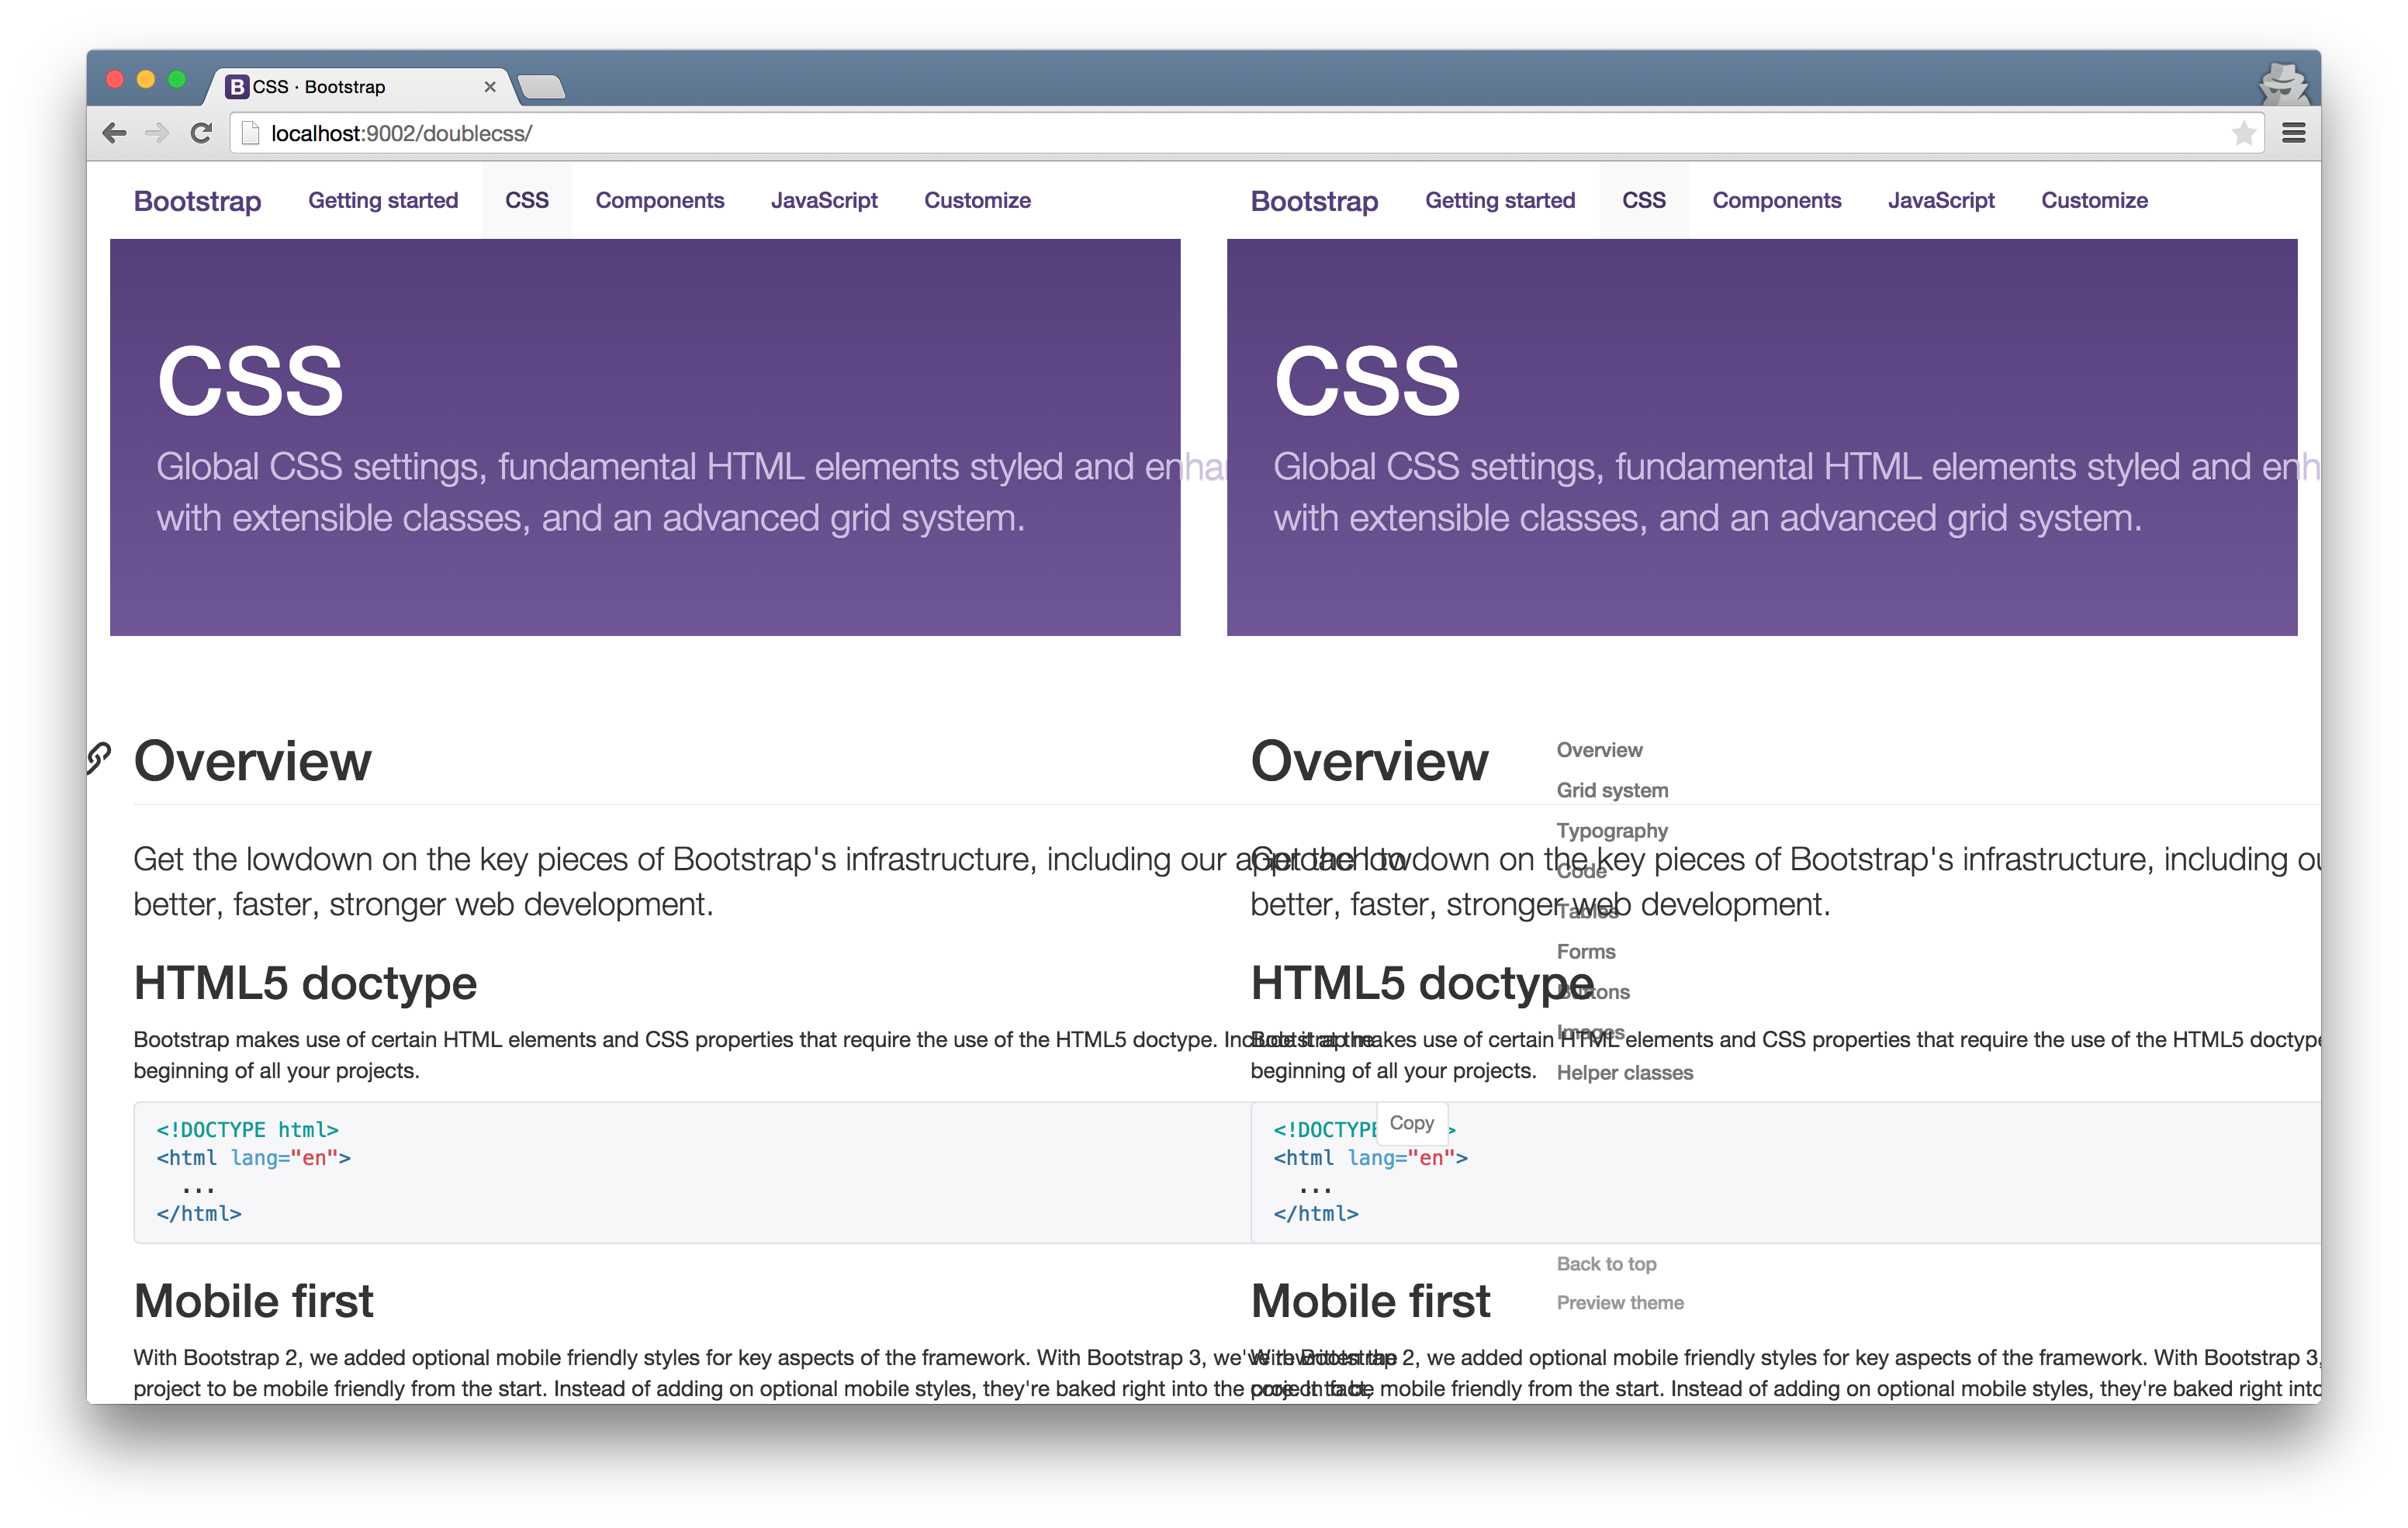
\includegraphics[width=\linewidth]{images/bootstrap-mq-header-small}
        \end{minipage}%
        \begin{minipage}{.5\textwidth}
          \centering
          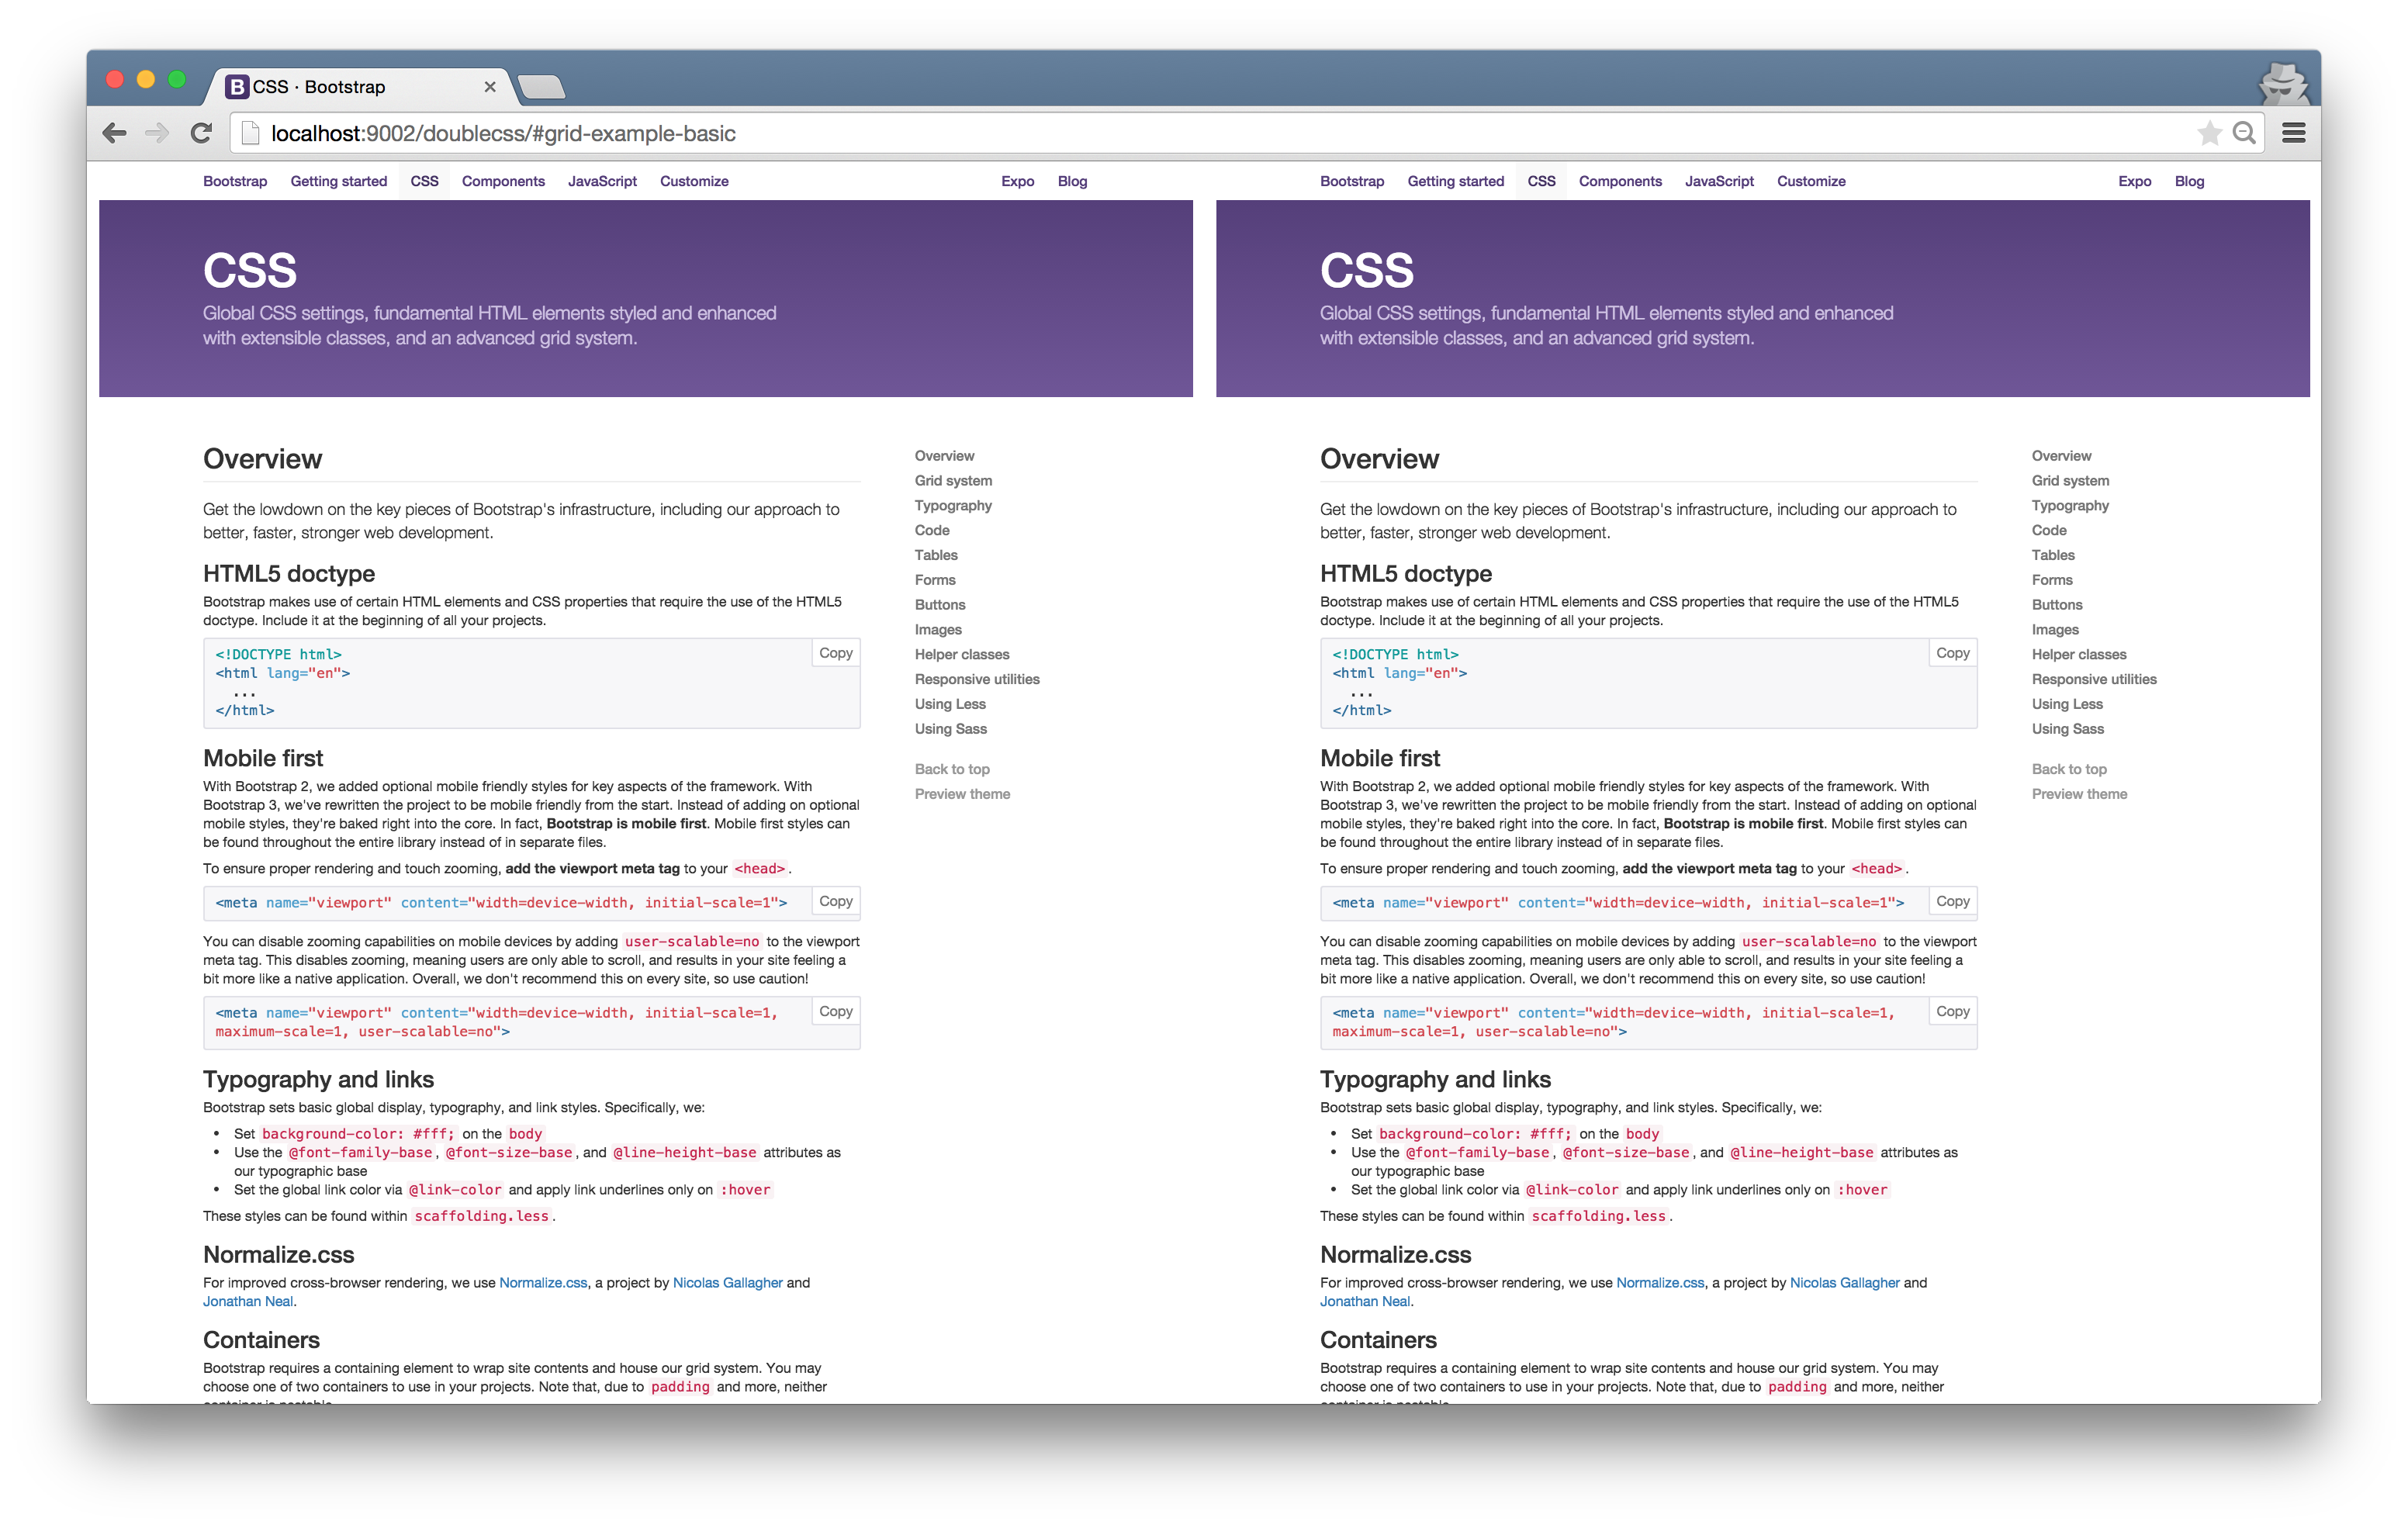
\includegraphics[width=\linewidth]{images/bootstrap-mq-header-big}
        \end{minipage}
        \caption{
          The \gls{responsive} classes of \gls{Bootstrap} cannot adapt to layout changes as shown with the two-column \gls{CSS} documentation page example.
          Both documentation instances use \gls{media queries}, which undesirably style both columns as if they each fill the whole \gls{viewport} width.
          Since the columns only fill half of the \gls{viewport} width and are styled as they both fill the whole \gls{viewport} width, the page appears broken as shown in the left figure.
          The page only behaves as desired if the \gls{viewport} width is large enough so that the width of each column is bigger than the largest \glslink{media queries}{media query} breakpoint, as shown in the right figure.
          See figure~\ref{fig:appendix-bootstrap-mq-header-small} and~\ref{fig:appendix-bootstrap-mq-header-big} of the appendix for the left and right figure in full scale, respectively.}
        \label{fig:eval-bootstrap-mq-broken}
      \end{figure}
      \todo{The right image should maybe show how it should look instead.}
      \todo{Not happy with the formulation "as if they fill the whole viewport width"}

      In order to make \gls{Bootstrap} behave as desired in any layouts the \gls{responsive} parts of the framework were modified to use element queries instead of \gls{media queries} by using \gls{ELQ}.
      Two \gls{Bootstrap} classes have been chosen to be treated as sub-\glspl{viewport} that are \code{elq-breakpoints} \glspl{element}: \code{container} and \code{container-fluid}.
      \todo{Not happy with calling containers as \glspl{viewport}}
      Both classes are used in \gls{Bootstrap} to define new parts of a page (e.g., a grid is required to have a container ancestor).
      They are also nestable, which makes them suitable to be used as sub-\glspl{viewport}.
      \todo{Not happy with calling containers for \glspl{viewport}. should come up with something better.}
      The \code{container} class centers content with fixed widths by different \gls{viewport} sizes, and the \code{container-fluid} uses the full available width.
      The idea is to have all \gls{responsive} classes conditionally styled with element queries by the size of the nearest ancestor container \gls{element}.
      This implies that all \glspl{element} with \gls{responsive} classes are converted to \code{elq-mirror} \glspl{element} since they need to mirror the breakpoints of the nearest ancestor \code{elq-breakpoints} element (i.e., a container \gls{element}).
      Since container \glspl{element} may be nested, \code{container} \glspl{element} are both \code{elq-mirror} and \code{elq-breakpoints} \glspl{element} (because \code{container} \glspl{element} also conditionally style themselves, as opposed to \code{container-fluid} \glspl{element}).
      Recall from section~\ref{sec:plugin-mirror} that it is beneficial for \gls{responsive} \glspl{element} to be \code{elq-mirror} \glspl{element} in order to not limit the element usage to a specific \gls{HTML} structure.

      \paragraph{Altering the style code}
      \gls{Bootstrap} mainly uses three width numbers for \gls{responsive} breakpoints: 768, 970 and 1170 pixels.
      Since the \gls{Bootstrap} \gls{CSS} is generated by the \gls{LESS} preprocessor, they are defined as constants as presented in listing~\ref{code:bootstrap-less-breakpoints}.
      \begin{lstlisting}[gobble=8,label={code:bootstrap-less-breakpoints},caption={The main breakpoints used by \gls{Bootstrap} defined as \gls{LESS} constants.},captionpos=b]]
        /* File "less/variables.less" of Bootstrap. */
        @screen-sm-min: 480px;
        @screen-md-min: 992px;
        @screen-lg-min: 1200px;
      \end{lstlisting}
      Notice that the numbers also include the \code{px} postfix.
      Recall from Section~\ref{sec:plugin-breakpoints} that the breakpoint classes added by the \code{elq-breakpoints} plugin do not include the \code{px} postfix by default (i.e., if an element is above 480 pixels the class would be \code{elq-width-above-480} and not \code{elq-width-above-480px}).
      Fortunately, the \code{elq-breakpoints} plugin may be configured to append a postfix to the breakpoint classes by the \code{postfix} option.
      By configuring the plugin to use \code{px} as postfix, the constants can be used seamlessly in element queries.
      As shown in listing~\ref{code:bootstrap-less-breakpoints-usage}, \gls{media queries} are easily replaced by element queries.
      \begin{lstlisting}[gobble=8,label={code:bootstrap-less-breakpoints-usage},caption={Media queries can easily be replaced with element queries. By using the \code{elq-breakpoints} postfix option; the breakpoint constants can be used directly in the selectors. Notice that only three lines have been altered.},captionpos=b]]
        /* File "less/grid.less" of Bootstrap. */

        // Original Boostrap using media queries.
        .container {
          .container-fixed();

          @media (min-width: @screen-sm-min) {
            width: @container-sm;
          }
          @media (min-width: @screen-md-min) {
            width: @container-md;
          }
          @media (min-width: @screen-lg-min) {
            width: @container-lg;
          }
        }

        // ELQ Bootstrap using element queries.
        .container {
          .container-fixed();

          &.elq-width-above-@{screen-sm-min} {
            width: @container-sm;
          }
          &.elq-width-above-@{screen-md-min} {
            width: @container-md;
          }
          &.elq-width-above-@{screen-lg-min} {
            width: @container-lg;
          }
        }
      \end{lstlisting}
      \todo{Write how many chars that differ?}
      By using the power of preprocessors, \gls{ELQ} element queries become as pleasant to work with as \gls{media queries}.
      In fact, only \textasciitilde50 lines out of \textasciitilde8500 lines of \gls{Bootstrap} \gls{LESS} code needed to be altered.
      Most changes were of the character shown in listing~\ref{code:bootstrap-less-breakpoints-usage}, which basically replaces the \glslink{media queries}{media query} syntax with the \gls{ELQ} element queries syntax.
      This is especially advantageous when keeping a \glslink{fork}{forked} project up to date with the original project, as fewer diverged lines implies a lowered risk of merge conflicts.

      \paragraph{Adding the \gls{ELQ} library}
      The altered \gls{Bootstrap} version depends on \gls{ELQ} including two plugins (\code{elq-breakpoints} and \code{elq-mirror}) and must therefore be included.
      \gls{ELQ} and the plugins could be bundled with the \gls{JavaScript} of \gls{Bootstrap}, but it was decided to keep them separated.
      \gls{Bootstrap}'s other dependency, jQuery, is also separated from the \gls{Bootstrap} \gls{JavaScript}.
      Since it is beneficial to not require changes to existing \gls{Bootstrap} empowered pages, all \gls{ELQ} element attributes are added with \gls{JavaScript}.
      The attributes could of course be written directly in the \gls{HTML} instead; the choice is up to the user.
      Listing~\ref{code:bootstrap-init-js} presents an example of such \gls{JavaScript} code that dynamically adds the required element attributes and initializes all \gls{responsive} \glspl{element}.
      \begin{lstlisting}[gobble=8,label={code:bootstrap-init-js},caption={Example of \gls{JavaScript} code that adds the required \gls{ELQ} attributes dynamically to all \gls{responsive} \glspl{element} and initializes them.},captionpos=b]]
        // Creating the ELQ instance needs to be done once.
        var elq = Elq();
        elq.use(elqBreakpoints, {
          postfix: "px"
        });
        elq.use(elqMirror);

        // This function initiates all responsive elements of the document.
        function init(elq) {
          // Find all elements that have responsive classes.
          var breakpointsElements = [...]; // body, .container-fluid, .navbar, ...
          var containerElements   = [...]; // .container
          var mirrorElements      = [...]; // .visible-xs, .col-md-1, .col-md-12, ...

          // Add all attributes for the elq-breakpoints elements.
          breakpointsElements.concat(containerElements).forEach(function (element) {
            element.setAttribute("elq", "");
            element.setAttribute("elq-breakpoints", "");
            element.setAttribute("elq-breakpoints-width", "480 768 992 1200");
          });

          // Add all attributes for the elq-mirror elements.
          mirrorElements.concat(containerElements).forEach(function (element) {
            element.setAttribute("elq", "");
            element.setAttribute("elq-mirror", "");
          });

          // .container elements are both elq-mirror and elq-breakpoints,
          // and therefore the noclasses option is added so that the plugins 
          // do not interfere with each other.
          containerElements.forEach(function (element) {
            element.setAttribute("elq-breakpoints", "noclasses");
          });

          var elements = breakpointsElements.concat(containerElements, mirrorElements);
          elq.start(elements);
        }

        // Init all responsive elements. This needs to be executed when 
        // new responsive elements are added.
        init(elq);
      \end{lstlisting}

      \paragraph{The result}
      Altering the \gls{LESS} code, including the \gls{ELQ} library, and the initiating \gls{JavaScript} is all that is required to make the double column documentation page behave as desired.
      Figure~\ref{fig:eval-bootstrap-mq-eq-header}, \ref{fig:eval-bootstrap-mq-eq-matrix} and \ref{fig:eval-bootstrap-mq-eq-grid} shows different sections of the double column documentation page empowered by \gls{ELQ} \gls{Bootstrap}.
      For reference, the same sections using the original \gls{Bootstrap} is also included that shows how they behave without element queries.
      As shown in the figures, the double column documentation page using the original \gls{Bootstrap} styles the two columns as if they both had the whole \gls{viewport} width available.
      Therefore the two columns intersect because some content \glspl{element} are styled wider than a column.
      The double column documentation page using \gls{ELQ} \gls{Bootstrap} on the other hand enables all \gls{responsive} \glspl{element} to style themselves according a parent container \gls{element}.
      Therefore, the two half-page columns detect that they only have half the \gls{viewport} width and style themselves accordingly.
      The visual result is the same as having two documentation sites of the original \gls{Bootstrap} in two \code{iframe} \glspl{element} as two columns (since \code{iframe} \glspl{element} creates a separate \gls{viewport}).
      \todo[inline]{Write that the original CSS documentation behaves as expected out of the box (not changes to the html)?}
      \todo[inline]{Write that such small code changes (also maybe state the total code changes of the repo) really eases merging of new updates to the upstream repo.}

      \begin{figure}[hp!]
        \centering
        \begin{minipage}{.5\textwidth}
          \centering
          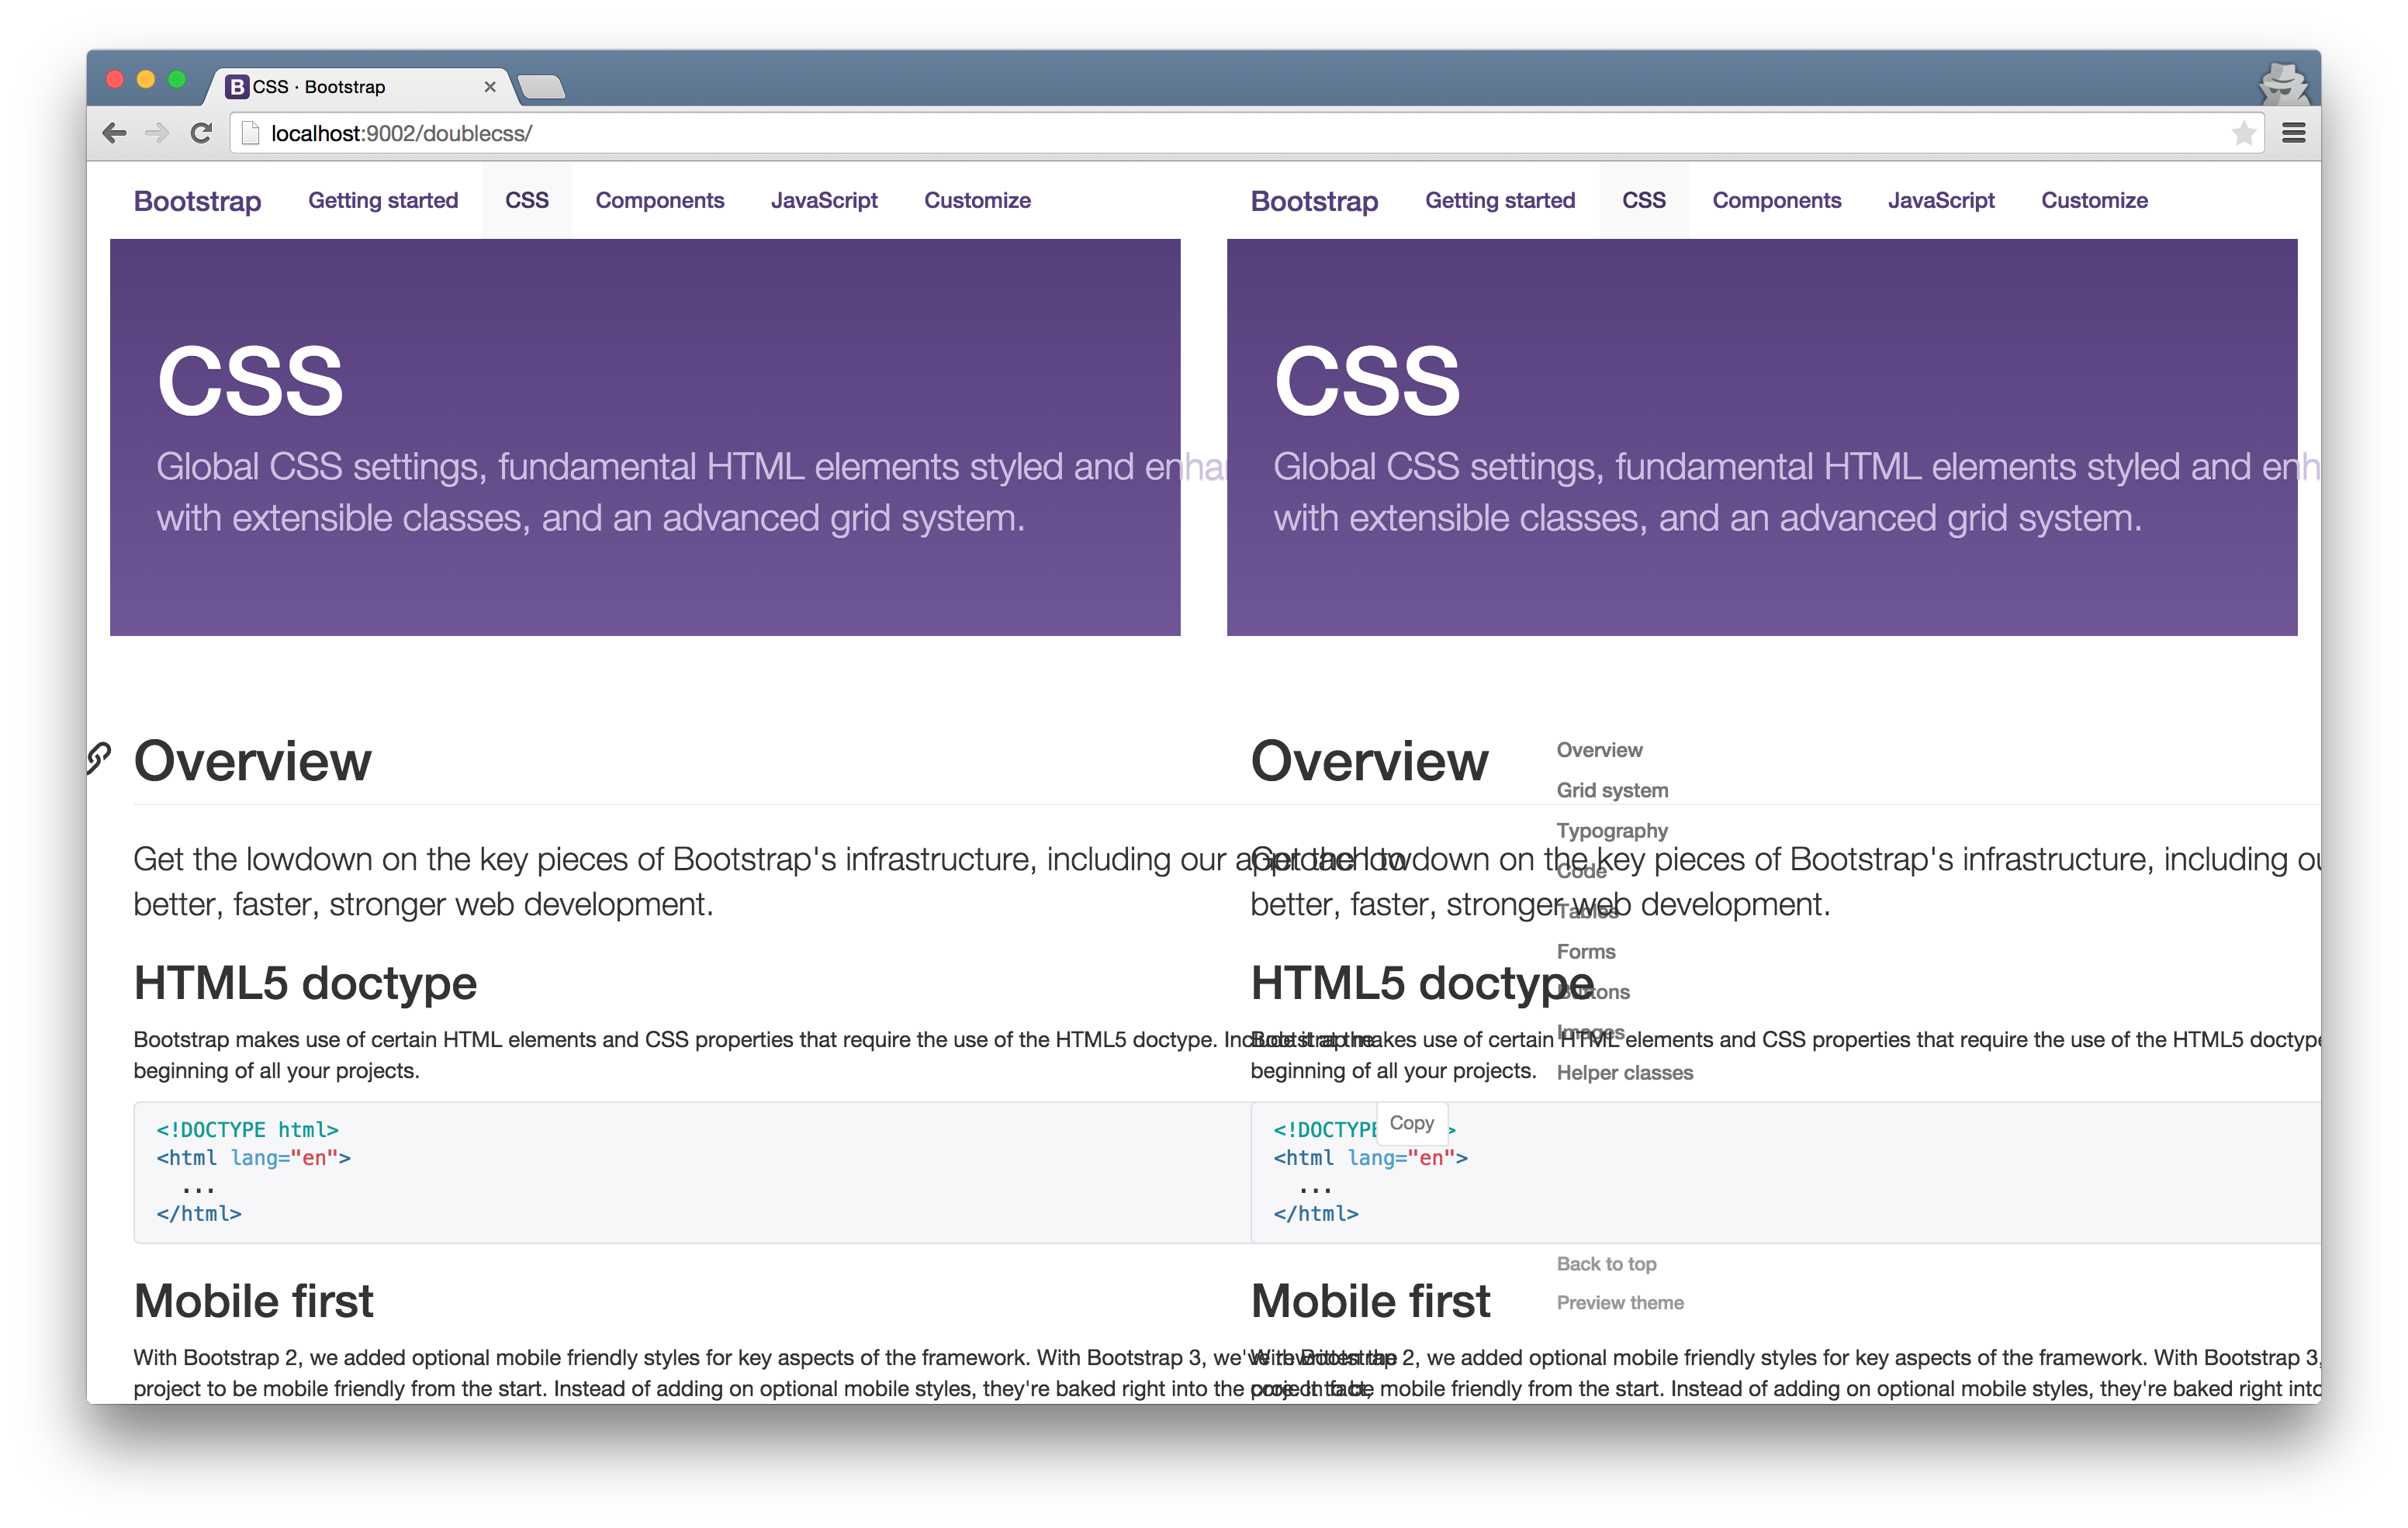
\includegraphics[width=\linewidth]{images/bootstrap-mq-header-small}
        \end{minipage}%
        \begin{minipage}{.5\textwidth}
          \centering
          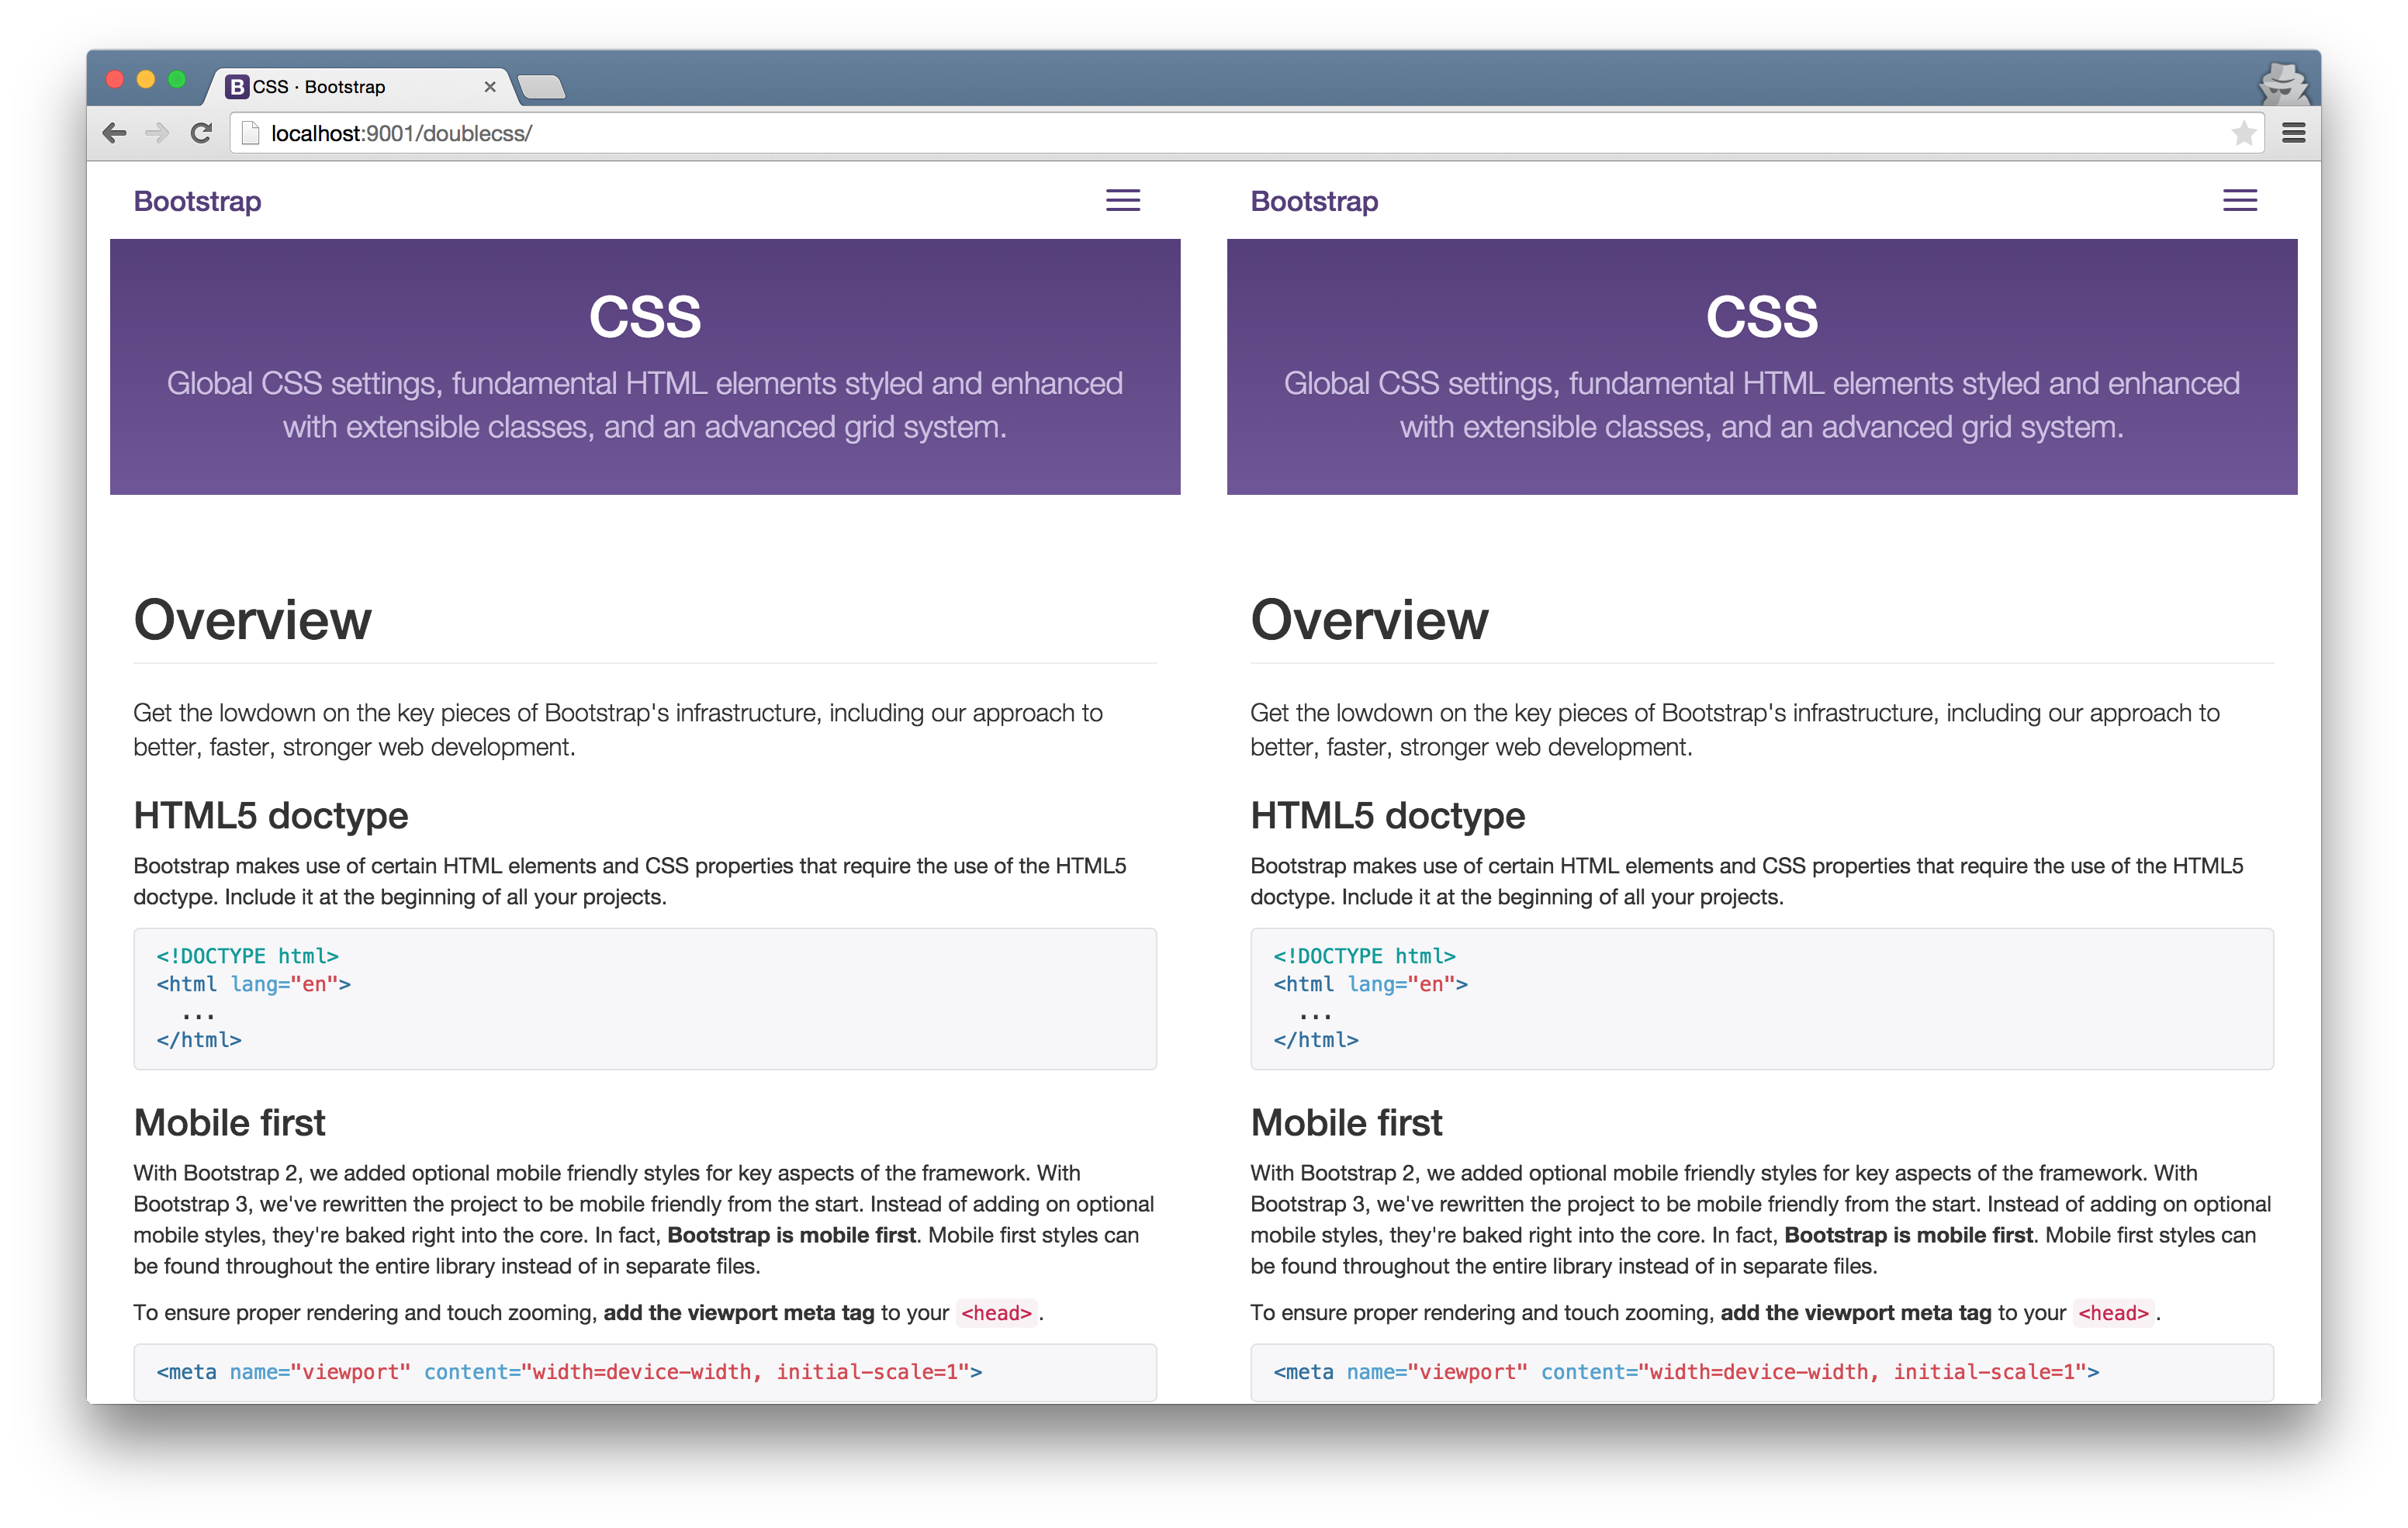
\includegraphics[width=\linewidth]{images/bootstrap-eq-header-small}
        \end{minipage}
        \caption{
          The left image shows the original \gls{Bootstrap} header, which is broken since the content of both columns are styled as if they had the full \gls{viewport} width.
          The right image shows same section of the same page, using \gls{ELQ} \gls{Bootstrap}.
          With element queries, both columns know that they only have half of the \gls{viewport} width and therefore style themselves accordingly.
          See figure~\ref{fig:appendix-bootstrap-mq-header-small} and~\ref{fig:appendix-bootstrap-eq-header-small} of the appendix for the left and right figure in full scale, respectively.}
        \label{fig:eval-bootstrap-mq-eq-header}
      \end{figure}

      \begin{figure}[htb!]
        \centering
        \begin{minipage}{.5\textwidth}
          \centering
          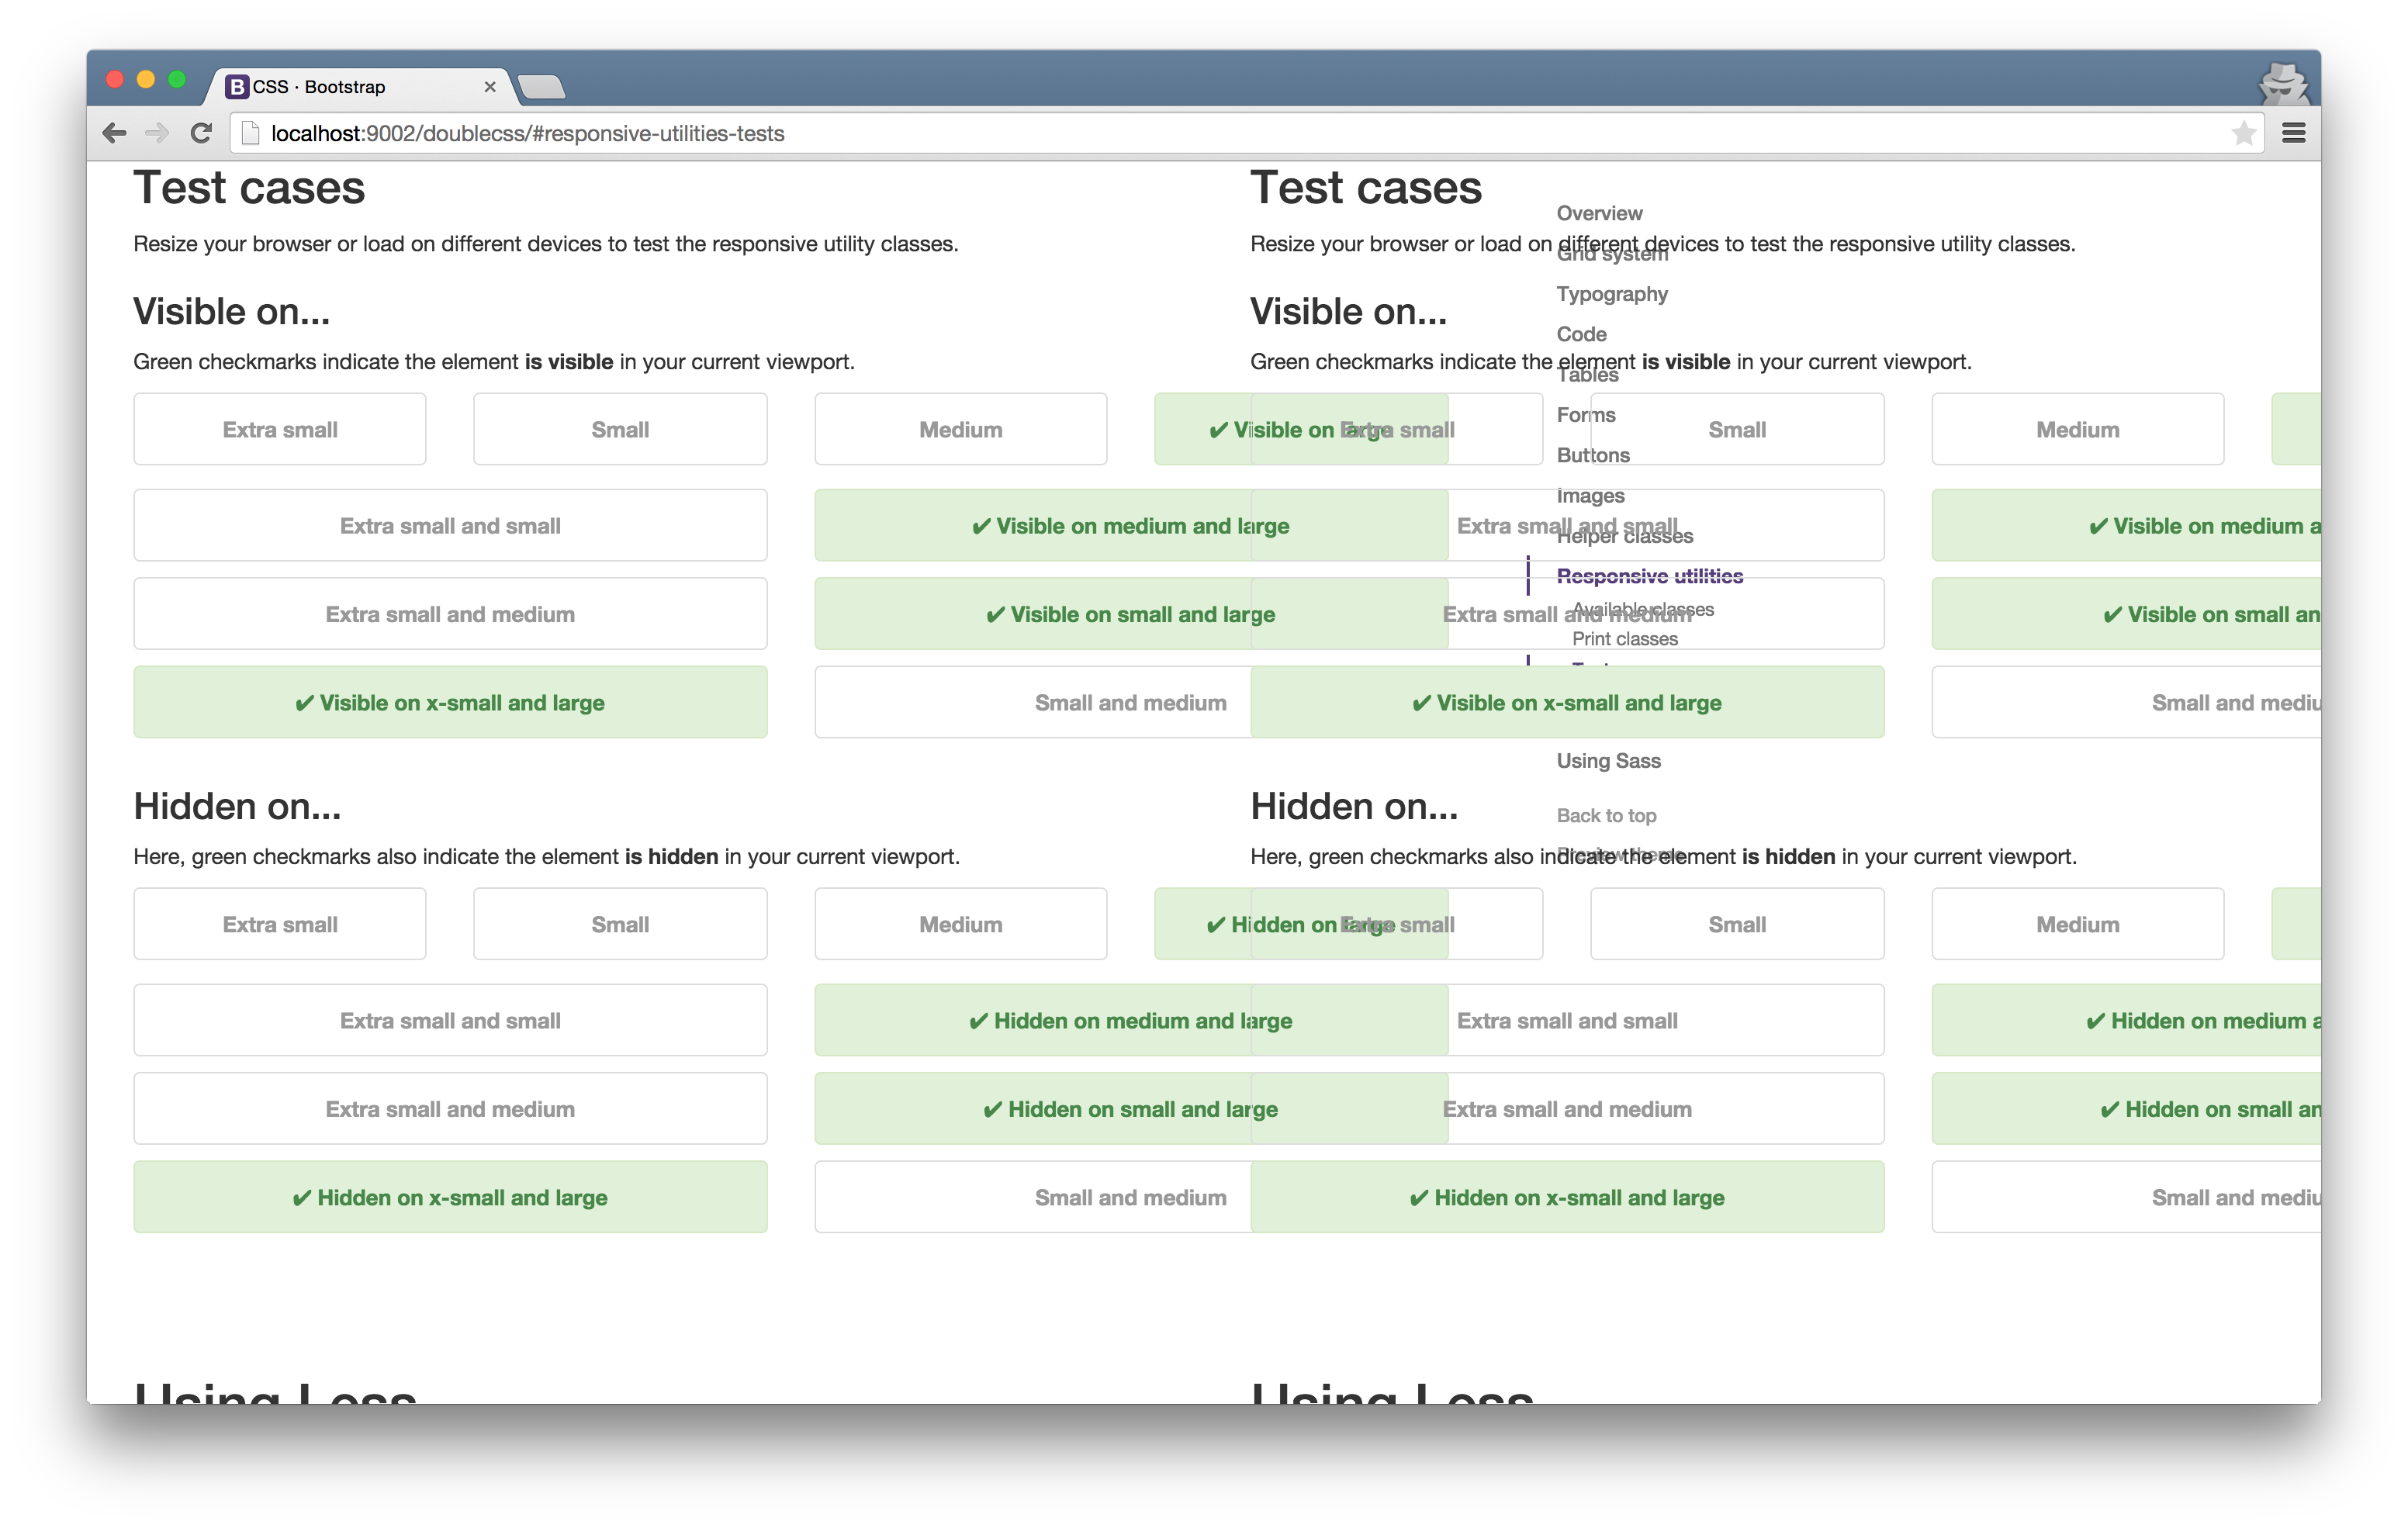
\includegraphics[width=\linewidth]{images/bootstrap-mq-matrix}
        \end{minipage}%
        \begin{minipage}{.5\textwidth}
          \centering
          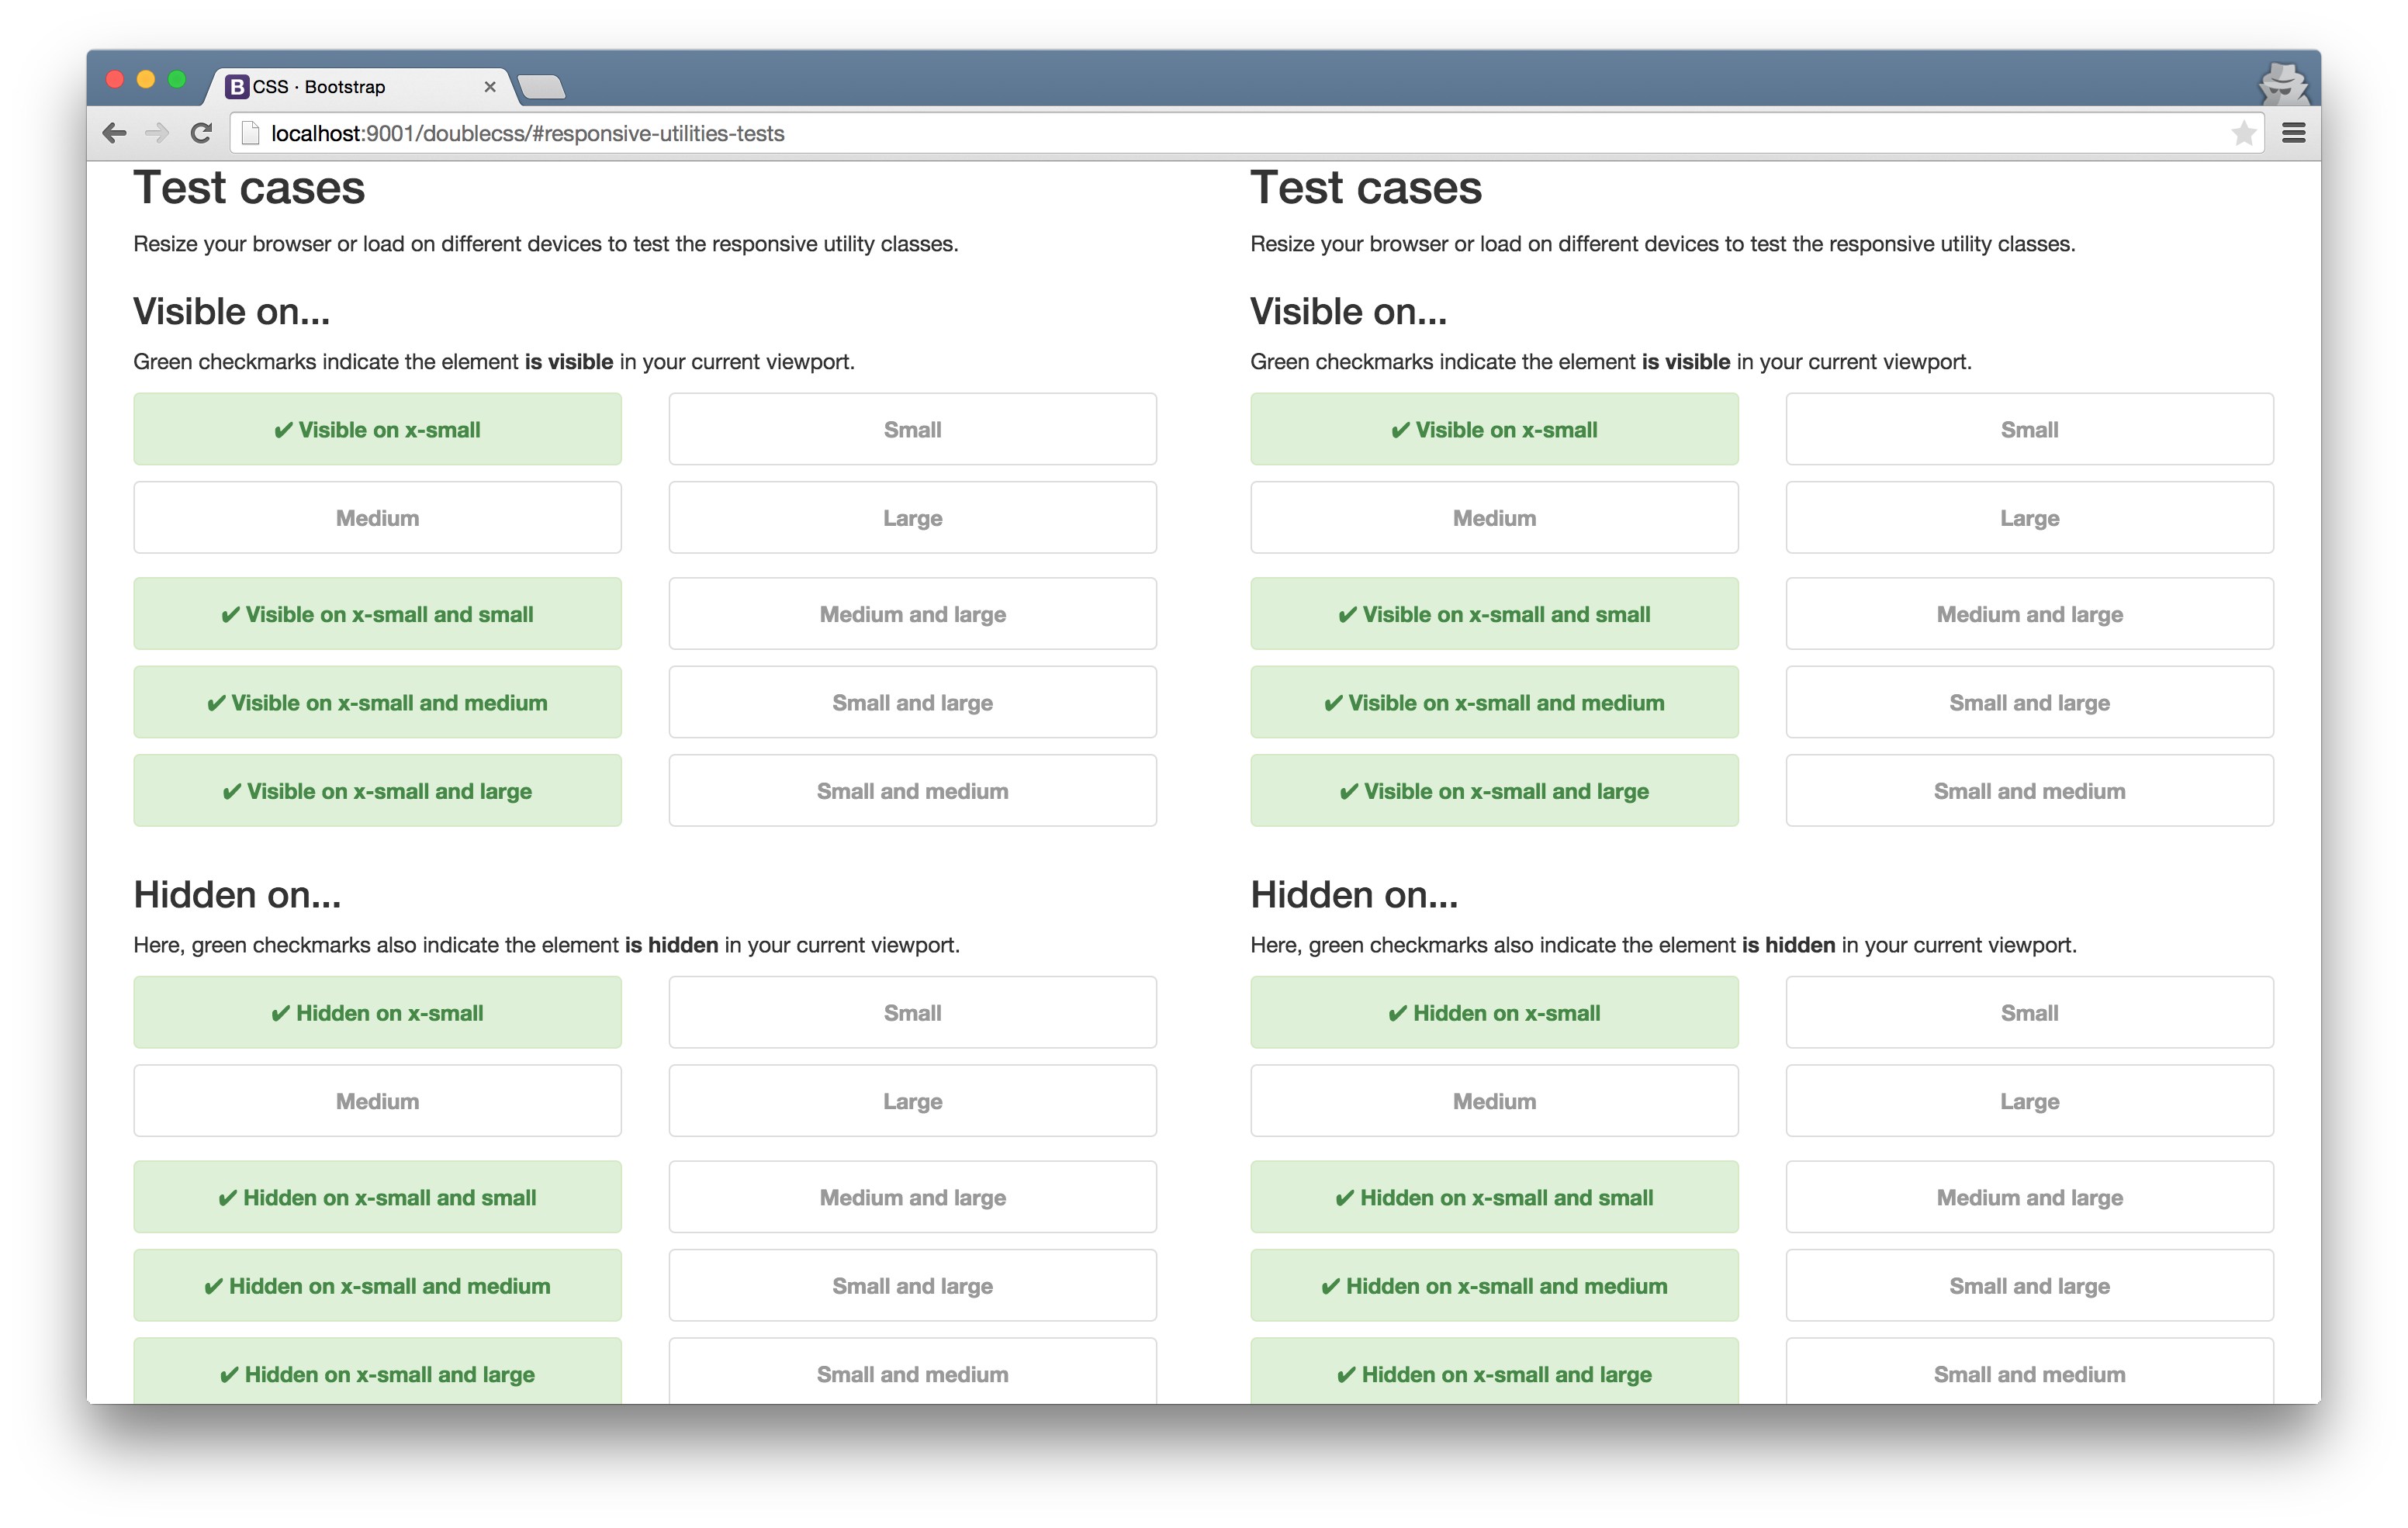
\includegraphics[width=\linewidth]{images/bootstrap-eq-matrix}
        \end{minipage}
        \caption{
          The left image shows the original \gls{Bootstrap} \gls{responsive} utilities classes matrix.
          Here it is clear that both columns are styled as if they each have the full \gls{viewport} width, as they display the large utility classes in green.
          The right image shows same section of the same page, using \gls{ELQ} \gls{Bootstrap}.
          Only the small utility classes are displayed in green as desired, since both columns only have half of the \gls{viewport} width available.
          See figure~\ref{fig:appendix-bootstrap-mq-matrix-small} and~\ref{fig:appendix-bootstrap-eq-matrix-small} of the appendix for the left and right figure in full scale, respectively.
        }
        \label{fig:eval-bootstrap-mq-eq-matrix}
      \end{figure}

      \begin{figure}[htb!]
        \centering
        \begin{minipage}{.5\textwidth}
          \centering
          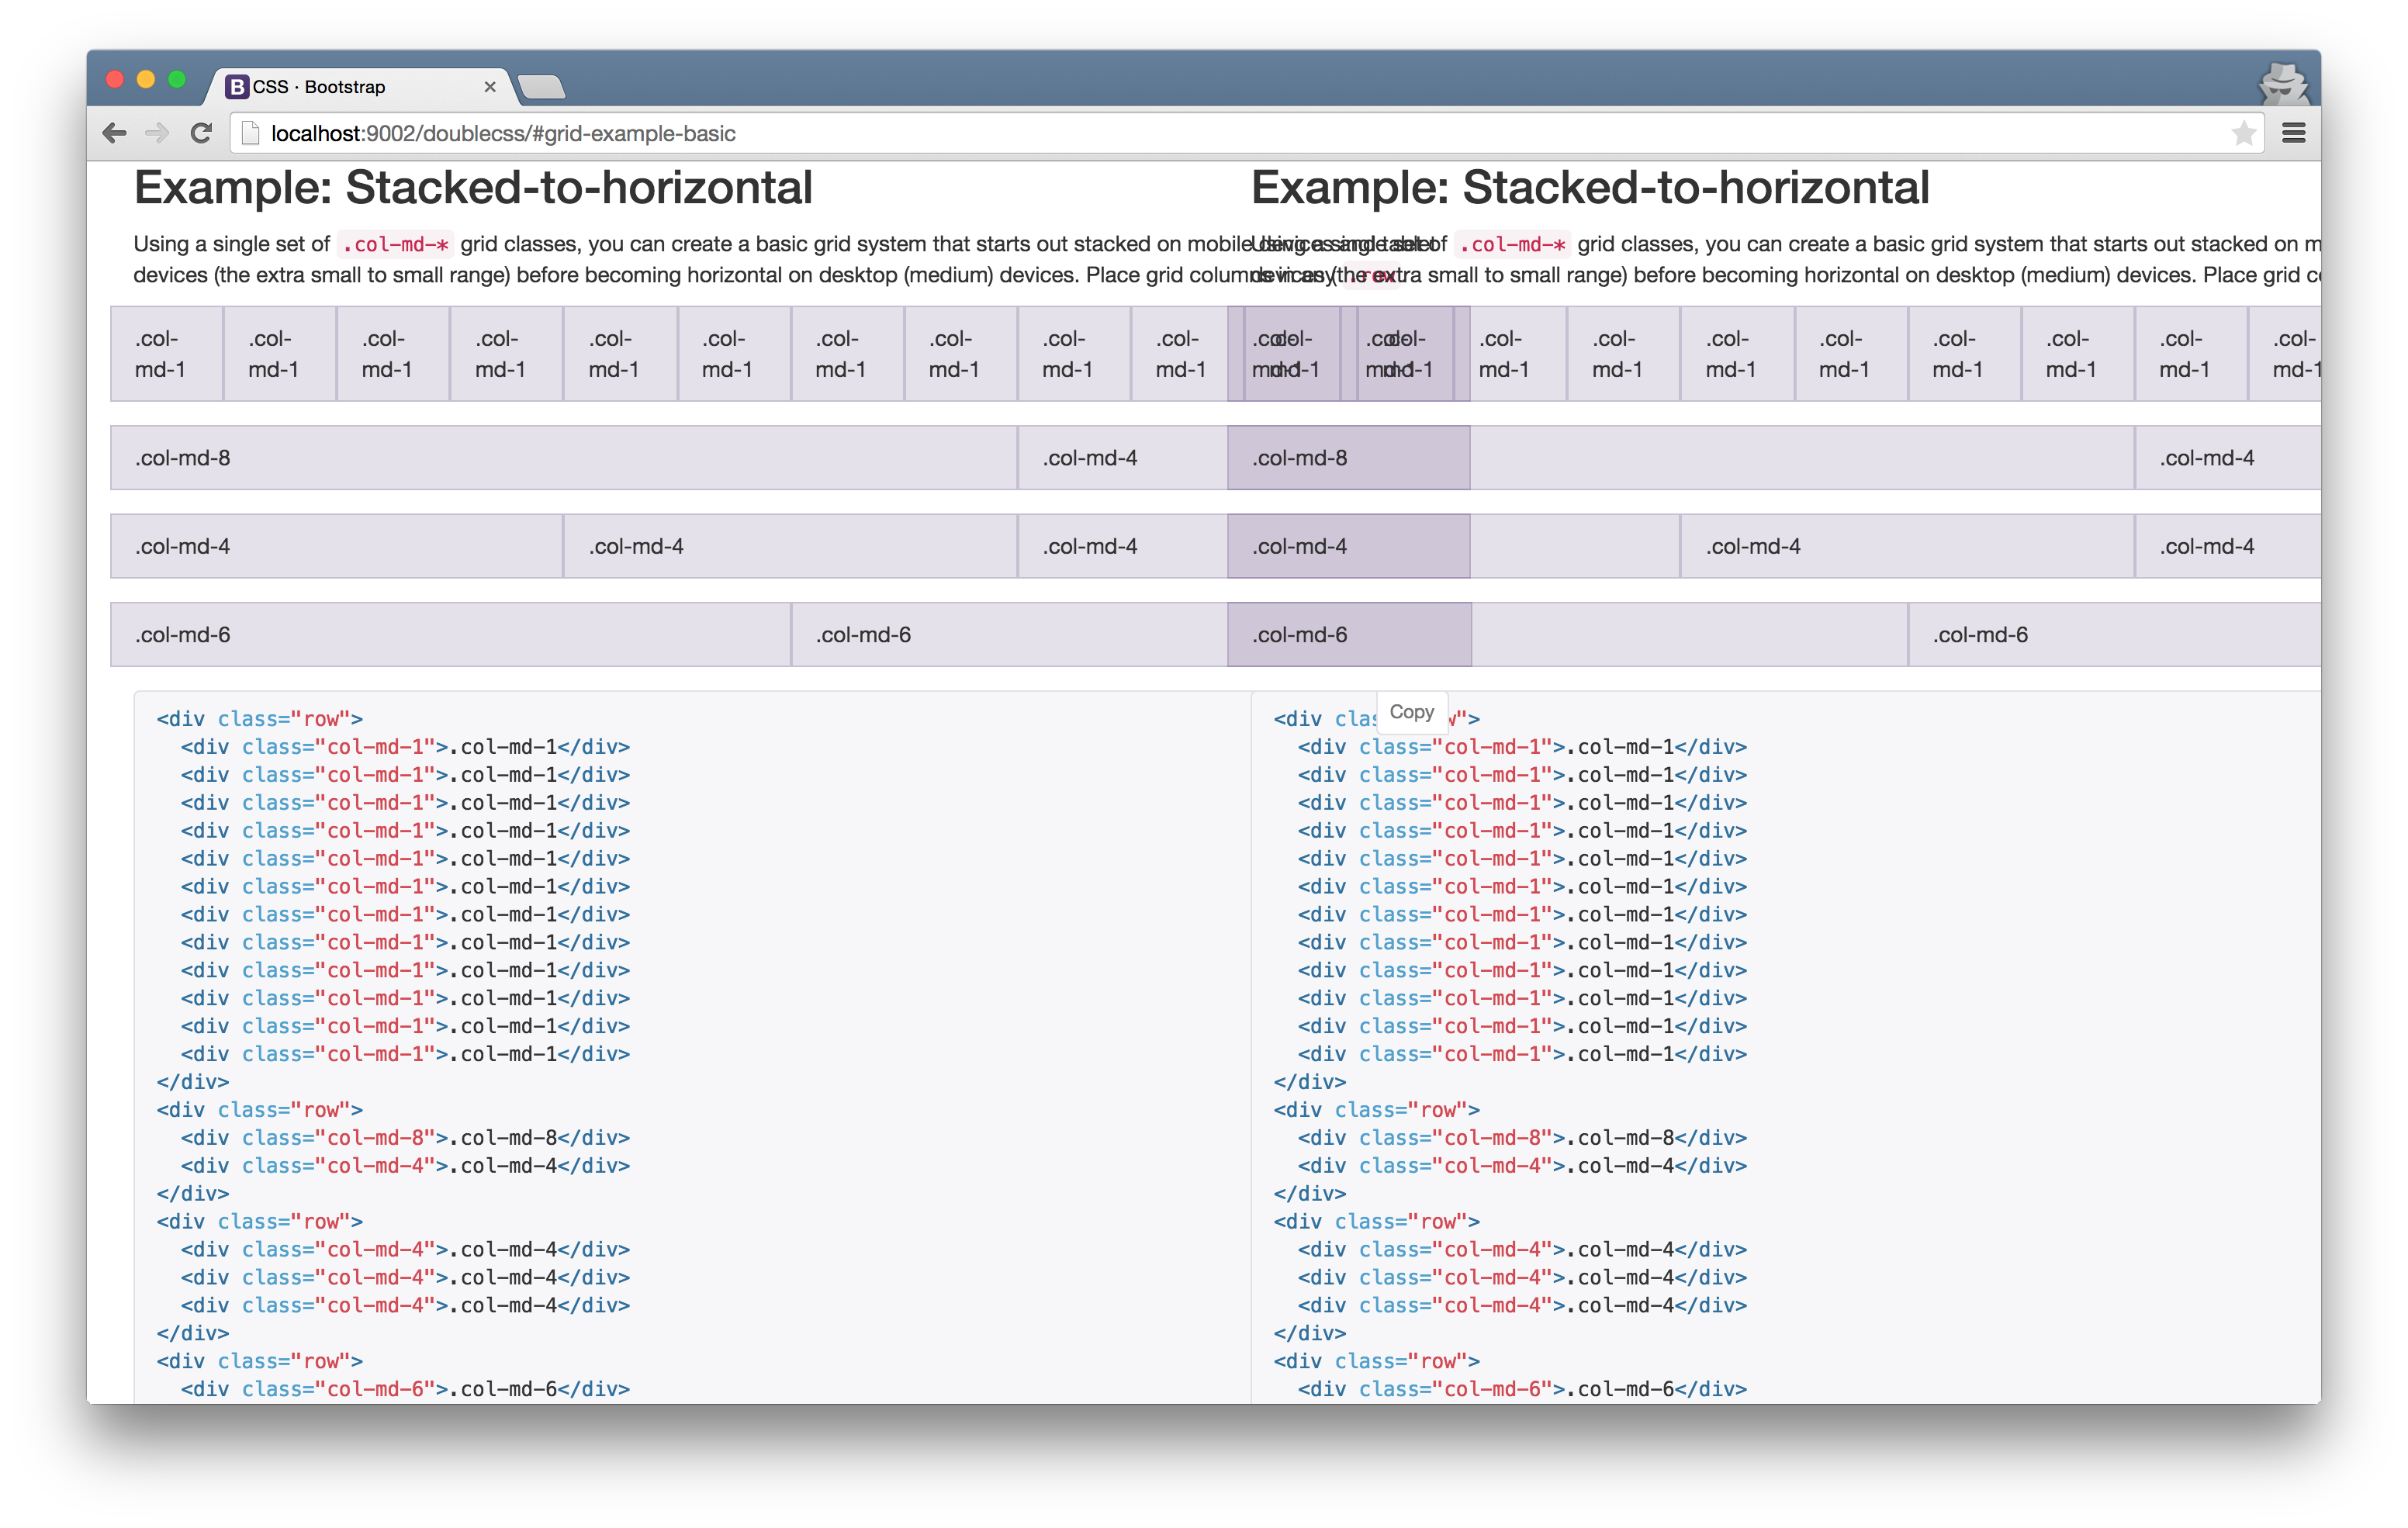
\includegraphics[width=\linewidth]{images/bootstrap-mq-grid}
        \end{minipage}%
        \begin{minipage}{.5\textwidth}
          \centering
          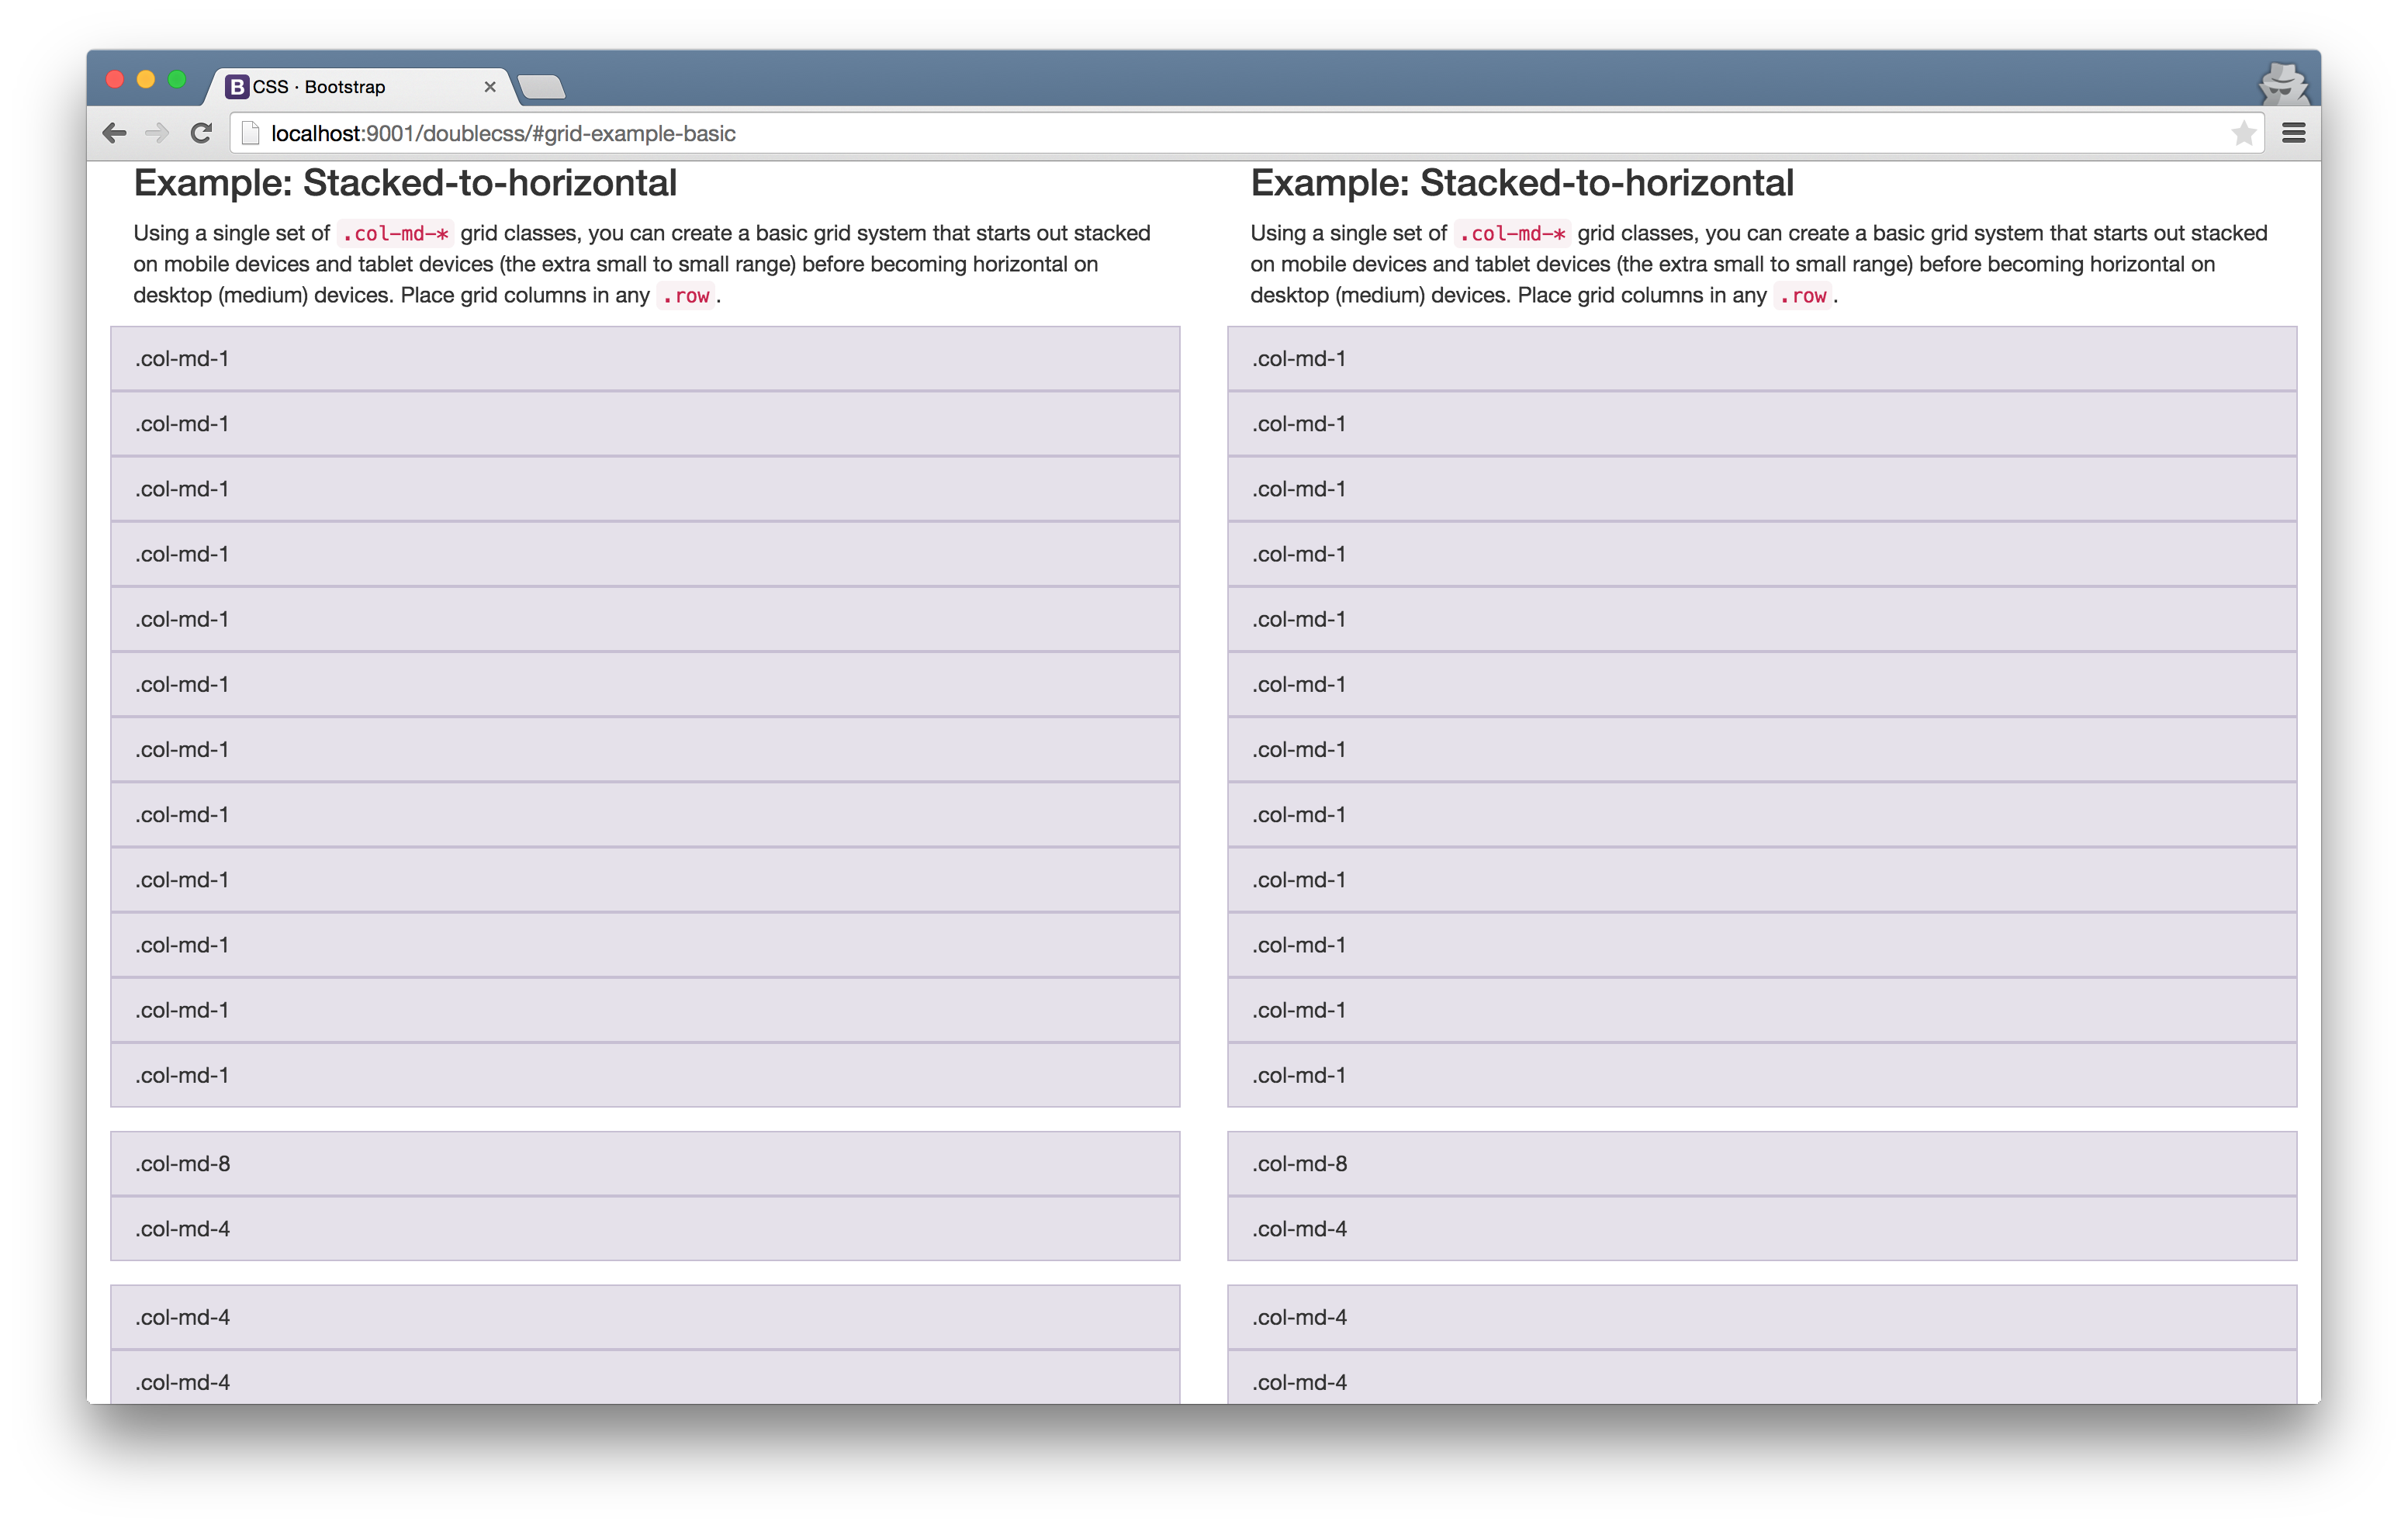
\includegraphics[width=\linewidth]{images/bootstrap-eq-grid}
        \end{minipage}
        \caption{
          The left image shows the original \gls{Bootstrap} \gls{responsive} grid.
          It is styled as if both columns have the full \gls{viewport} width available, and therefore the grids intersect.
          The right image shows same section of the same page, using \gls{ELQ} \gls{Bootstrap}.
          The grids detect that only the half \gls{viewport} width is available, and styles themselves accordingly.
          See figure~\ref{fig:appendix-bootstrap-mq-grid-small} and~\ref{fig:appendix-bootstrap-eq-grid-small} of the appendix for the left and right figure in full scale, respectively.
        }
        \label{fig:eval-bootstrap-mq-eq-grid}
      \end{figure}

      \todo[inline]{Write that the original Bootstrap CSS documentation page worked out of the box with the ELQ Bootstrap version}

    \FloatBarrier
    %%%%%%%%%%%%%%%%%%%%%%%%%%%%%%%%%%%%%%%%%%%%%%%%%%%%%%%%%%%%%%%%%%%%%%%%%%%%%%%%%%%%%%%%%%%%%%%%%%%%%%%%%%%%%%%%%%%%%%%%%%%%%%%%%%%%%%%%%%%%%%%%%%%%%%%%%%%%%%%%%%%%%%%%%%%%%%%%%%%%%%%%%%%%%%%%%%%%%%%%%%%%%%%%%%%%%%%%%%%%%%%%%%%%%%%%%%%%%%%%%%%%%%%%%%%%%%%%%%%%%%%%%%%%%%%%%%%%%%%%%%%%%%%%%%%%%%%%%%%%%%%%%%%%%%%%%%%%%%%%%%%%%%%%%%%%%%%%%%%%%%%%%%%%%%%%%%%%%%%%%%
    %%%%%%%%%%%%%%%%%%%%%%%%%%%% Performance
    %%%%%%%%%%%%%%%%%%%%%%%%%%%%%%%%%%%%%%%%%%%%%%%%%%%%%%%%%%%%%%%%%%%%%%%%%%%%%%%%%%%%%%%%%%%%%%%%%%%%%%%%%%%%%%%%%%%%%%%%%%%%%%%%%%%%%%%%%%%%%%%%%%%%%%%%%%%%%%%%%%%%%%%%%%%%%%%%%%%%%%%%%%%%%%%%%%%%%%%%%%%%%%%%%%%%%%%%%%%%%%%%%%%%%%%%%%%%%%%%%%%%%%%%%%%%%%%%%%%%%%%%%%%%%%%%%%%%%%%%%%%%%%%%%%%%%%%%%%%%%%%%%%%%%%%%%%%%%%%%%%%%%%%%%%%%%%%%%%%%%%%%%%%%%%%%%%%%%%%%%%
    \section{Performance}\label{sec:eval-performance}\label{sec:eval-perf-erd}
      The following tests were performed on a computer with a 2.5 GHz processor and 16 GB of memory\footnote{The serial number of the computer is C02N4G9TG3QD and the vendor is Apple Inc. CPU: 2.5 GHz Intel Core i7. Memory: 16 GB 1600 MHz DDR3. GPU: Intel Iris Pro 1536 MB.}.
      The library has been tested in the following \glspl{browser}: Chrome 42.0.2311.152, FireFox 37.0.1 and Safari 8.0.6.
      Measurements and graphs show evaluations performed in Chrome unless stated otherwise.

      % Have this here?
      % Since the algorithm neither interacts with the \gls{DOM}, handles any large data structures, or performs any heavy computations it is very fast.
      % It takes \textasciitilde0.02 ms to execute the \code{isUpdateCyclic} function.
      % \todo{Should this measurement be given in eval? But then eval will be really small?}
      % See figure~\ref{} for a timeline of the \code{elq-breakpoints} plugin handling a resize event, where it is visually shown how insignificant the impact of the cycle detector system has on the total performance.

      \todo[inline]{Include evaluation about the cycle detector?}
      \todo[inline]{Write about the new "noclasses" option, and maybe flesh out the interplugin API section?}
      \todo[inline]{Write that as ELQ is plugin-based, it makes sense to measure the core subsystems by themselves and the plugins enabling element queries in different setups.}
      \todo[inline]{Have to measure how elq-breakpoints handles large amount of elements. It might suffor from layout thrashing since might read/write the DOM at invalid stages of the erd subsystem.}
      \todo[inline]{Actually since elq-breakpoints is batch-processed, no layout thrashing occurs. However, two disjunct layouts are performed (one for the erd system and one for the plugin) which could theoretically be merged.}
      \todo[inline]{Philipp: If possible, show graphs for other browsers than Chrome.}
      \todo[inline]{Write about Bootstrap performance here.}

      
      %\subsection{Element resize detection}\label{sec:eval-perf-erd}
        This section evaluates the performance of the object-based and scroll-based solutions to detecting \gls{element} resize events described in Section~\ref{sec:imp_erd}.
        The optimized \gls{ELQ} version of the scroll-based solution is also be evaluated.
        Since the element resize detection subsystem performs the heaviest tasks, only the performance of that subsystem is evaluated in detail.
        The other subsystems entail no significant performance penalties.
        \todo{Remove this, and analyze the different subsystems in detail: erd, cycle detector, elq-breakpoints, etc.}

        The object-based solution performs well when detecting resize events.
        However, injecting \code{object} \glspl{element} is quite a heavy task.
        See figure~\ref{fig:erd-original-object} for graphs that show the performance of the object-based solution.
        As shown by the graphs, the injection can be performed with adequate performance as long as the number of \glspl{element} is low.
        The solution does not scale well as the number of element increases.
        \todo{Maybe be less pessimistic as Safari might have to use the object solution?}
        \begin{figure}[ht]
          \tiny
          \begin{center}
            \begin{minipage}[t]{.5\textwidth}
              \vspace{0pt}
              \centering
                \begin{tikzpicture}
                  \begin{axis}[
                      width=\textwidth, % Scale the plot to \linewidth
                      grid=major, % Display a grid
                      grid style={dashed,gray!30}, % Set the style
                      xlabel=Number of \glspl{element}, % Set the labels
                      ylabel=Injection time,
                      y unit=s, % Set the respective units
                      legend style={at={(0.5,-0.20)},anchor=north} % Put the legend below the plot
                    ]
                    \addplot+[red, mark options={red}] table[x=n elements,y=injection time,col sep=comma] {./data/erd-object-original.csv};
                    \legend{Object-based solution}
                  \end{axis}
                \end{tikzpicture}
            \end{minipage}%
            \begin{minipage}[t]{.5\textwidth}
              \vspace{0pt}
              \centering
              \begin{tikzpicture}
                \begin{axis}[
                    width=\textwidth, % Scale the plot to \linewidth
                    grid=major, % Display a grid
                    grid style={dashed,gray!30}, % Set the style
                    xlabel=Number of \glspl{element}, % Set the labels
                    ylabel=Heap memory usage,
                    y unit=MB, % Set the respective units
                    legend style={at={(0.5,-0.20)},anchor=north} % Put the legend below the plot
                  ]
                  \addplot+[red, mark options={red}]
                  % add a plot from table; you select the columns by using the actual name in
                  % the .csv file (on top)
                  table[x=n elements,y=memory,col sep=comma] {./data/erd-object-original.csv};
                  \legend{Object-based solution}
                \end{axis}
              \end{tikzpicture}
            \end{minipage}
          \caption{The injection performance of the object-based solution. The left graph shows the injection time. The right graph shows the heap memory used when all \code{object} \glspl{element} have been injected.}
          \label{fig:erd-original-object}
          \end{center}
        \end{figure}

        % See figure~\ref{fig:erd-elq-scroll} for graphs that show how the \gls{ELQ} scroll-based solution performs compared to the other solutions.
        % As evident in the figure, the optimized \gls{ELQ} solution has significantly reduced installation times compared to the other two.
        % The \gls{ELQ} solution also scales better, as more clearly shown in figure~\ref{fig:erd-solutions-regressed} that includes polynomial regression graphs for all three solutions.
        % Both scroll-based solutions have the same memory footprint (i.e., too low for reliable measurements).

        The scroll-based solution also performs well when detecting resize events.
        As no \code{object} \glspl{element} are injected the memory footprint is reduced significantly, which improves the injection performance.
        See figure~\ref{fig:erd-original-scroll} for graphs that show how the both solutions perform compared to each other.
        It is clear that the scroll-based solution both performs and scales better than the object-based solution during injection.        
        The amount of memory used by the scroll-based solution is so low that reliable measurements could not be gathered, as the number of \glspl{element} was not high enough to affect the memory usage noticeably.
        \begin{figure}[ht]
          \tiny
          \begin{center}
            \begin{minipage}[t]{.5\textwidth}
              \vspace{0pt}
              \centering
                \begin{tikzpicture}
                  \begin{axis}[
                      width=\textwidth, % Scale the plot to \linewidth
                      grid=major, % Display a grid
                      grid style={dashed,gray!30}, % Set the style
                      xlabel=Number of \glspl{element}, % Set the labels
                      ylabel=Injection time,
                      y unit=s, % Set the respective units
                      legend style={at={(0.5,-0.20)},anchor=north} % Put the legend below the plot
                    ]
                    \addplot+[orange, mark=square*, mark options={orange}] table[x=n elements,y=injection time,col sep=comma] {./data/erd-scroll-original.csv};
                    \addlegendentry{Scroll-based solution}
                  \end{axis}
                \end{tikzpicture}
            \end{minipage}%
            \begin{minipage}[t]{.5\textwidth}
              \vspace{0pt}
              \centering
              \begin{tikzpicture}
                \begin{axis}[
                    width=\textwidth, % Scale the plot to \linewidth
                    grid=major, % Display a grid
                    grid style={dashed,gray!30}, % Set the style
                    xlabel=Number of \glspl{element}, % Set the labels
                    ylabel=Injection time,
                    y unit=s, % Set the respective units
                    legend style={at={(0.5,-0.20)},anchor=north} % Put the legend below the plot
                  ]
                  \addplot+[red, mark options={red}] table[x=n elements,y=injection time,col sep=comma] {./data/erd-object-original.csv};
                  \addplot+[orange, mark options={orange}] table[x=n elements,y=injection time,col sep=comma] {./data/erd-scroll-original.csv};
                  \addlegendentry{Object-based solution}         
                  \addlegendentry{Scroll-based solution}
                \end{axis}
              \end{tikzpicture}
            \end{minipage}
          \caption{The injection performance of the scroll-based element resize detection solution provided by \cite{eq_imp_css-element-queries} and originally created by \cite{backalley}. The left graph shows the injection time of the scroll-based solution. The right graph also includes the object-based solution for reference. The heap memory usage graph has been omitted as the memory usage for the scroll-based solution is near constant.}
          \label{fig:erd-original-scroll}
          \end{center}
        \end{figure}

        Recall that the scroll-based solution was rewritten and optimized; which is referred to as the \gls{ELQ} version of the scroll-based solution.
        By avoiding \gls{layout thrashing}, the injection performance was improved significantly.
        See figure~\ref{fig:erd-elq-scroll} for graphs that show how it performs compared to the other solutions.
        As evident in the figure, the optimized \gls{ELQ} solution has significantly reduced injection times compared to the other two.
        It achieves a 32-fold speedup compared to the object-based solution and a 13-fold speedup compared to the scroll-based solution when preparing 500 \glspl{element} for resize detection.
        The \gls{ELQ} solution also scales better, as more clearly shown in figure~\ref{fig:erd-solutions-regressed} that includes polynomial regression graphs for all three solutions.
        Both scroll-based solutions have the same memory footprint (i.e., too low for reliable measurements).
        \begin{figure}[ht!]
          \tiny
          \begin{center}
            \begin{minipage}[t]{.5\textwidth}
              \vspace{0pt}
              \centering
                \begin{tikzpicture}
                  \begin{axis}[
                      yticklabel style={
                              /pgf/number format/fixed,
                              /pgf/number format/precision=5
                      },
                      scaled y ticks=false,
                      width=\textwidth, % Scale the plot to \linewidth
                      grid=major, % Display a grid
                      grid style={dashed,gray!30}, % Set the style
                      xlabel=Number of \glspl{element}, % Set the labels
                      ylabel=Injection time,
                      y unit=s, % Set the respective units
                      legend style={at={(0.5,-0.20)},anchor=north} % Put the legend below the plot
                    ]
                    \addplot+[blue, mark=diamond*, mark options={blue}] table[x=n elements,y=injection time,col sep=comma] {./data/erd-scroll-elq.csv};
                    \addlegendentry{ELQ scroll-based solution}
                  \end{axis}
                \end{tikzpicture}
            \end{minipage}%
            \begin{minipage}[t]{.5\textwidth}
              \vspace{0pt}
              \centering
              \begin{tikzpicture}
                \begin{axis}[
                    width=\textwidth, % Scale the plot to \linewidth
                    grid=major, % Display a grid
                    grid style={dashed,gray!30}, % Set the style
                    xlabel=Number of \glspl{element}, % Set the labels
                    ylabel=Injection time,
                    y unit=s, % Set the respective units
                    legend style={at={(0.5,-0.20)},anchor=north} % Put the legend below the plot
                  ]
                  \addplot+[red, mark options={red}] table[x=n elements,y=injection time,col sep=comma] {./data/erd-object-original.csv};
                  \addplot+[orange, mark options={orange}] table[x=n elements,y=injection time,col sep=comma] {./data/erd-scroll-original.csv};
                  \addplot+[blue, mark=diamond*, mark options={blue}] table[x=n elements,y=injection time,col sep=comma] {./data/erd-scroll-elq.csv};

                  \addlegendentry{Object-based solution}
                  \addlegendentry{Scroll-based solution}
                  \addlegendentry{ELQ scroll-based solution}
                \end{axis}
              \end{tikzpicture}
            \end{minipage}
          \caption{The injection performance of the optimized \gls{ELQ} scroll-based element resize detection solution. The left graph shows the injection time of the \gls{ELQ} scroll-based solution. The right graph shows all three solutions for comparison. The heap memory usage graph has been omitted as the memory usage for the scroll-based solutions are near constant.}
          \label{fig:erd-elq-scroll}
          \end{center}
        \end{figure}
        \begin{figure}[ht!]
          \tiny
          \begin{center}
            \centering
            \begin{tikzpicture}
              \begin{axis}[
                  width=0.6\textwidth, % Scale the plot to \linewidth
                  grid=major, % Display a grid
                  grid style={dashed,gray!30}, % Set the style
                  xlabel=Number of \glspl{element}, % Set the labels
                  ylabel=Injection time,
                  y unit=s, % Set the respective units
                  legend style={at={(0.5,-0.20)},anchor=north} % Put the legend below the plot
                ]
                \addplot+[red, mark options={red}] table[x=n elements,y=injection time,col sep=comma] {./data/erd-object-original.csv};
                \addplot+[orange, mark options={orange}] table[x=n elements,y=injection time,col sep=comma] {./data/erd-scroll-original.csv};
                \addplot+[blue, mark options={blue}] table[x=n elements,y=injection time,col sep=comma] {./data/erd-scroll-elq.csv};
                \addplot[dashed,red,domain=1:1500,samples=100] {5.567042796*10^(-6)*x^2 + 4.680174396*10^(-3)*x + 6.495754669*10^(-3)};
                \addplot[dashed,orange,domain=1:1500,samples=100] {4.533208873*10^(-6)*x^2 + 6.320377596*10^(-4)*x + 2.289566005*10^(-2)};
                \addplot[dashed,blue,domain=1:1500,samples=100] {4.071740702*10^(-8)*x^2 + 1.823749404*10^(-4)*x + 1.527042267*10^(-2)};
                \addlegendentry{Original object-based solution}
                \addlegendentry{Scroll-based solution}
                \addlegendentry{ELQ scroll-based solution}
              \end{axis}
            \end{tikzpicture}
          \caption{The injection performance of all three solutions including graph predictions by polynomial regression.}
          \label{fig:erd-solutions-regressed}
          \end{center}
        \end{figure}

        \paragraph{FireFox and Safari}
        As shown, great performance can be achieved with the optimized \gls{ELQ} scroll-based solution in Chrome.
        Unfortunately, there is no silver bullet to observing element resize events; as the other \glspl{browser} behave differently.
        See table~\ref{table:erd-layout-engines} for the performance of the object-based and scroll-based solutions operating on 100 \glspl{element} in different \glspl{browser}.
        The \gls{ELQ} scroll-based solution is preferred for Chrome, as the injection is 32-fold faster (when operating on 500 \glspl{element}) than the object-based solution while the resize detection performance is the same for both solutions.
        In FireFox, the object-based solution detects resize events 2-fold faster than the \gls{ELQ} scroll-based solution when operating on 100 \glspl{element} (still, 100 ms for detecting resize events is acceptable).
        However, the injection time needed for the object-based solution is 5.5-fold of the time needed for the \gls{ELQ} scroll-based solution.
        The \gls{ELQ} scroll-based solution is therefore probably desired in FireFox for the general use case (as described in Section~\ref{sec:eq-definitions}).
        In Safari, the \gls{ELQ} scroll-based solution detects resize events in 800 ms while the object-based solution detects them in 25 ms, which of course is unacceptable.
        Unfortunately, the injection time needed for the object-based solution is 3-fold slower than the \gls{ELQ} scroll-based solution.
        Since a delay of 800 ms when detecting resize events is undesired in most use cases, the object-based solution is preferred is Safari.
        Recall from Section~\ref{sec:imp_erd} that this is due to WebKit and Gecko not being able to queue the scroll mutation operations as Blink does.
        \begin{table}[ht]\center
          \tiny
          \begin{tabular}[t]{ l l l l l l l }
            \multirow{2}{*}{Layout engine} & \multicolumn{2}{c}{Injection} & \multicolumn{2}{c}{Resize detection} \\
            & scroll & object & scroll & object \\
            \hline
            \gls{Blink}   & \textbf{30 ms}   & 600 ms    & 30 ms   & 30 ms           \\
            \gls{Gecko}   & \textbf{200 ms}  & 1100 ms   & 100 ms  & \textbf{50 ms}  \\
            \gls{WebKit}  & \textbf{100 ms}  & 300 ms    & 800 ms  & \textbf{25 ms}  \\
          \end{tabular}
          \caption{Performance of the object-based and \gls{ELQ} scroll-based solutions in different \glspl{layout engine} when operating on 100 \glspl{element}.}
          \label{table:erd-layout-engines}
        \end{table}

        \todo[inline]{Present perf statistics of other browsers? Firefox still seems to favor the scroll solution (but less performant) while Safari semms to favors the object solution.}
        \todo[inline]{Show graph for resize detection also.}
        \todo[inline]{Graphs for FireFox, IE and Safari?}

  %%%%%%%%%%%%%%%%%%%%%%%%%%%%%%%%%%%%%%%%%%%%%%%%%%%%%%%%%%%%%%%%%%%%%%%%%%%%%%%%%%%%%%%%%%%%%%%%%%%%%%%%%%%%%%%%%%%%%%%%%%%%%%%%%%%%%%%%%%%%%%%%%%%%%%%%%%%%%%%%%%%%%%%%%%%%%%%%%%%%%%%%%%%%%%%%%%%%%%%%%%%%%%%%%%%%%%%%%%%%%%%%%%%%%%%%%%%%%%%%%%%%%%%%%%%%%%%%%%%%%%%%%%%%%%%%%%%%%%%%%%%%%%%%%%%%%%%%%%%%%%%%%%%%%%%%%%%%%%%%%%%%%%%%%%%%%%%%%%%%%%%%%%%%%%%%%%%%%%%%%%
  %%%%%%%%%%%%%%%%%%%%%%%%%%%% Related work
  %%%%%%%%%%%%%%%%%%%%%%%%%%%%%%%%%%%%%%%%%%%%%%%%%%%%%%%%%%%%%%%%%%%%%%%%%%%%%%%%%%%%%%%%%%%%%%%%%%%%%%%%%%%%%%%%%%%%%%%%%%%%%%%%%%%%%%%%%%%%%%%%%%%%%%%%%%%%%%%%%%%%%%%%%%%%%%%%%%%%%%%%%%%%%%%%%%%%%%%%%%%%%%%%%%%%%%%%%%%%%%%%%%%%%%%%%%%%%%%%%%%%%%%%%%%%%%%%%%%%%%%%%%%%%%%%%%%%%%%%%%%%%%%%%%%%%%%%%%%%%%%%%%%%%%%%%%%%%%%%%%%%%%%%%%%%%%%%%%%%%%%%%%%%%%%%%%%%%%%%%%
  \chapter{Related work}\label{ch:related-work}
    There are numerous \gls{third-party} element queries \gls{JavaScript} libraries, which this chapter aims to list and analyze.
    Since many of them share the same characteristics, they are classified and analyzed in groups.
    A constraint-based approach is presented more in depth as it differs from the other libraries.

    Identified libraries that directly or indirectly enables element queries are presented in table~\ref{table:approaches-classifications}.
    The table also includes the classification of each library and some additional comments.
    It should be noted that most of the current approaches are combinations of different classes.
    The characteristics that they are classified after are the following:
    \begin{itemize}
      \item \textbf{Syntax}:  Libraries can either require custom syntax or valid syntax.
                              Custom syntax is considered to be invalid syntax since it does not conform to \gls{web} language standards (custom \gls{CSS} is the most common case of custom syntax).
                              Libraries that do no require custom syntax are considered to have valid syntax.
      \item \textbf{Page type}: All libraries support static pages, and some also support dynamic pages.
                                Static pages do not change layout at runtime, and therefore no \gls{element} resize detection or element queries library runtime is needed.
                                Dynamic pages may change layout at runtime, and therefore needs an element queries library runtime with \gls{element} resize detection.
      \item \textbf{Resize detection}:  Libraries need to detect \gls{element} resize events for dynamic layouts, and there are three levels of detection support for elements: \gls{viewport} only, non-void \glspl{element}, and arbitrary \glspl{element}.
                                        It should be noted that this only reflects the theoretical support of \glspl{element}; in practice many libraries have issues and bugs that make them unable to detect all \gls{element} resize events.
    \end{itemize}
    
    \begin{table}[ht]\center
      \tiny
      \begin{tabular}[t]{ l p{3cm} l l l p{3cm} }
        \multicolumn{2}{l}{Implementation} & Syntax & Resize detection & Page type & Comments \\
        \hline
        \cite{eq_imp_magichtml} &             MagicHTML &                                   Invalid &   - &                          Static &    Compiles invalid CSS to valid CSS at server side. \\
        \cite{eq_imp_eqcss} &                 EQCSS &                                       Invalid &   \Gls{viewport} only &        Dynamic     \\
        \cite{eq_imp_prollyfill-min-width} &  Element Media Queries &                       Invalid &   Non-void \glspl{element} &   Dynamic &   Flow-based element resize detection. \\
        \cite{eq_imp_localised-css} &         Localised CSS &                               Invalid &   Arbitrary \glspl{element} &  Dynamic &   Polling-based element resize detection. \\
        \cite{eq_imp_gss} &                   Grid Style Sheets 2.0 &                       Invalid &   Arbitrary \glspl{element} &  Dynamic &   Using the Cassowary constraints solver. \\
        \cite{eq_imp_classquery} &            Class Query &                                 Valid &     - &                          Static &    Writes \gls{media queries} to style on load. \\
        \cite{eq_imp_breakpointsjs} &         breakpoints.js &                              Valid &     \Gls{viewport} only &        Dynamic &   \\
        \cite{eq_imp_mediaclass} &            MediaClass &                                  Valid &     \Gls{viewport} only &        Dynamic &   Inline JS syntax. \\
        \cite{eq_imp_elementquery} &          ElementQuery &                                Valid &     \Gls{viewport} only &        Dynamic &   \\
        \cite{eq_imp_responsive-elements} &   Responsive Elements &                         Valid &     \Gls{viewport} only &        Dynamic &   \\
        \cite{eq_imp_sickles} &               SickleS &                                     Valid &     \Gls{viewport} only &        Dynamic &   Parses CSS. \\
        \cite{eq_imp_responsive-elements-2} & Responsive Elements &                         Valid &     \Gls{viewport} only &        Dynamic &   \\ 
        \cite{eq_imp_breaks2000} &            breaks2000 &                                  Valid &     \Gls{viewport} only &        Dynamic &   \\
        \cite{eq_imp_eqjs} &                  eq.js &                                       Valid &     \Gls{viewport} only &        Dynamic &   \\
        \cite{eq_imp_element-queries} &       Element Queries &                             Valid &     Non-void \glspl{element} &   Dynamic &   Object-based element resize detection. \\
        \cite{eq_imp_css-element-queries} &   CSS Element Queries &                         Valid &     Non-void \glspl{element} &   Dynamic &   Scroll-based element resize detection. \\
        \cite{eq_imp_selector_queries} &      Selector queries and responsive containers &  Valid &     Arbitrary \glspl{element} &  Dynamic &   Polling. \\
      \end{tabular}
      \caption{Classification of related element queries libraries.}
      \label{table:approaches-classifications}
    \end{table}
    % \cite{eq_imp_magichtml}             Invalid syntax. Semi-automatic. Static.
    % \cite{eq_imp_eqcss}                 Invalid syntax. Semi-automatic. Dynamic.
    % \cite{eq_imp_localised-css}         Invalid syntax. Automatic (with polling). Dynamic. Runtime parsing of CSS. Unfinished.
    % \cite{eq_imp_classquery}            Valid syntax.   Static. Writes media queries to style on load.
    % \cite{eq_imp_breakpointsjs}         Valid syntax.   Semi-Automatic (viewport + load). Dynamic. JS-centric approach.
    % \cite{eq_imp_mediaclass}            Valid syntax (custom inline JS syntax). Semi-automatic (seems like load only). Dynamic.
    % \cite{eq_imp_elementquery}          Valid syntax.   Semi-automatic. Dynamic.
    % \cite{eq_imp_responsive-elements}   Valid syntax.   Semi-Automatic. Dynamic.
    % \cite{eq_imp_sickles}               Valid syntax.   Semi-automatic. Part of bootstrap-like library. No JS API, instead parses CSS.
    % \cite{eq_imp_responsive-elements-2} Valid syntax.   Semi-automatic. Dynamic.
    % \cite{eq_imp_breaks2000}            Valid syntax.   Semi-automatic. Dynamic.
    % \cite{eq_imp_selector_queries}      Valid syntax.   Semi-automatic. Dynamic.
    % \cite{eq_imp_element-queries}       Valid syntax.   Automatic. Dynamic.
    % \cite{eq_imp_eqjs}                  Valid syntax.   Automatic. Dynamic
    % \cite{eq_imp_css-element-queries}   Valid syntax.   Automatic. Dynamic. Parses CSS.
    % \cite{eq_imp_prollyfill-min-width}  Invalid syntax. Automatic. Dynamic. Parses CSS.
    % \cite{eq_imp_gss}

    \todo{Did I miss this one? \url{https://github.com/jonathantneal/hitch-element-queries}}
    
    \paragraph{Invalid syntax}
    The libraries \cite{eq_imp_magichtml,eq_imp_eqcss,eq_imp_prollyfill-min-width,eq_imp_localised-css,eq_imp_gss} have in common that they require developers to write custom (invalid) \gls{CSS}.
    Since they no longer conform to the \gls{CSS} standard, new features can be supported through the custom \gls{CSS}.
    As shown by \cite{eq_imp_eqcss,eq_imp_gss} quite advanced features can be implemented this way.
    Additionally, adding new \gls{CSS} features implies that it is possible to implement a solution to element queries that does not require any changes to the \gls{HTML}, which may be preferable since all styling then can be written in \gls{CSS} (which is the purpose of \gls{CSS}).
    However, there are numerous drawbacks with libraries that require invalid \gls{CSS}.
    
    First, it requires a compilation step in order to produce valid \gls{CSS} that \glspl{layout engine} understand.
    This can either be done at server side or in the \gls{browser} at runtime.
    The advantage of having the compilation step at server side is increased performance since the \gls{browser} understands the \gls{CSS} directly when it has been retrieved.
    Server side compilation implies that the layout of the page cannot be changed at runtime and is therefore only useful for static pages.
    By instead having the compilation step at runtime, dynamic layouts can be used since element queries may be re-evaluated on layout changes.
    However, the performance impact of having the compilation step at runtime can be significant for the following reasons:
    \begin{itemize}
      \item The received \gls{CSS} cannot be understood by the \gls{browser}, and therefore all parsing and reasoning about it has to be postponed until the library script executes.
      Note that \glspl{layout engine} could in theory parse the \gls{CSS} and perform speculative selector matching while waiting for other parts of the page to finish (such as executing scripts), which cannot be done with invalid \gls{CSS}.
      \item When the library script executes it has to parse the custom \gls{CSS} --- a process which is most likely slower than \gls{native} parsing.
      \item When parsed, the library needs to apply its logic to the parsed \gls{CSS} and produce valid \gls{CSS}. The produced \gls{CSS} needs to be applied to the \gls{document} by mutating the \gls{DOM}.
      \todo{Write about reentrant HTML and layout thrashing etc?}
      \item The \gls{layout engine} needs to parse the \gls{CSS} added to the \gls{DOM}, which means that the styles of the page is parsed twice.
      \item The custom parser engine needs to be included in the page, which implies a larger library script size.
    \end{itemize}
    
    Second, by not conforming to \gls{CSS} standards many tools such as preprocessors, validators and linters are no longer compatible.
    Also, editors and other code-displaying tools are not able to understand the syntax and are therefore not able to highlight the code properly.
    It should be noted that it is in some cases possible to create plugins to such tools to extend their capabilities.

    Third, The custom \gls{API} and parser needs to be kept up to date with \gls{CSS} standards in order to make sure new features of \gls{CSS} are supported and that they are not conflicting with the custom \gls{API}.

    \paragraph{Resize detection}
    As shown in table~\ref{table:approaches-classifications}, most libraries simply observe the \gls{viewport} resize event, which may be enough for static pages.
    However, observing element resize events is desired for pages that change layout during runtime.
    The libraries \cite{eq_imp_localised-css,eq_imp_selector_queries,eq_imp_prollyfill-min-width,eq_imp_gss,eq_imp_element-queries,eq_imp_css-element-queries} have in common that they observe \glspl{element} for resize events.
    The libraries \cite{eq_imp_localised-css,eq_imp_selector_queries} use polling to detect element resize events, and therefore support arbitrary element resize detection.
    However, as presented in Section~\ref{sec:imp_erd}, polling is undesired.
    \todo{Write why again?}

    The three remaining libraries uses three different injection solutions, as described in Section~\ref{sec:imp_erd}, to detect element resize events; \cite{eq_imp_element-queries} uses the object-based solution, \cite{eq_imp_prollyfill-min-width} uses the flow-based solution, and \cite{eq_imp_css-element-queries} uses the scroll-based solution.
    According to the evaluation in Section~\ref{sec:eval-performance}, all three libraries are less performant than the element resize detection system used in \gls{ELQ}.
    Also, recall from Section~\ref{sec:imp_erd} that the flow-based and scroll-based solutions both have limitations and bugs.

    \paragraph{Constraint-based approach}
    Shortly after the introduction of \gls{CSS} by the \gls{W3C}, a proposal for \gls{CCSS} was submitted as a more general and flexible alternative to \gls{CSS} \cite{badros1999constraint}.
    As the name suggests, the idea of \gls{CCSS} is to layout \glspl{document} by constraints that would imply an unifying implementation mechanism (i.e., using a constraint solver).
    The constraint-based approach provides extended features and reduced complexity compared to \gls{CSS} according to the authors.
    The Cassowary\footnote{Cassowary is an incremental constraint solving toolkit that solves systems of linear equalities and inequalities. See \url{http://sourceforge.net/projects/cassowary/} for more information.} constraint solver was used (among other tools) to solve the constraints for the demonstration implementation of \gls{CCSS}.
    In 2011, Apple released their Auto Layout\footnote{For more information about Apple's Auto Layout, see \url{https://developer.apple.com/library/ios/documentation/UserExperience/Conceptual/AutolayoutPG/Introduction/Introduction.html}.} technology that uses a similar constraint-based approach.
    Apple's implementation also uses the Cassowary algorithms to solve the constraints.
    The Grid Style Sheets library \cite{eq_imp_gss} builds upon the ideas of \gls{CCSS} and uses a \gls{JavaScript} port\footnote{See \url{https://github.com/slightlyoff/cassowary.js} for the \gls{JavaScript} port of Cassowary that is used by the Grid Style Sheets library.} of Cassowary to solve the constraints at runtime.
    The library also adapted Apple's \gls{VFL} to specify layout constraints.
    While not directly offering element queries, the library enables the possibility to conditionally style elements by \gls{element} criteria and thus makes it a good candidate to solve the problem of \gls{responsive} modules.
    However, the library has two major issues: performance and browser compatibility \cite{gss_issue}.
    One approach to resolve both issues is to precompute the layout in a compilation step at the server.
    However, as earlier stated, precompiling styles implies static layouts.
    There are other approaches discussed that would increase the performance, but they also limit the dynamism of the page layout.
    Additionally, the library evaluates all \glspl{element} on \gls{DOM} mutations using the \code{MutationObserver} \gls{API}, which does not detect all element resize events as discussed in Section~\ref{sec:imp_erd}.

    \todo[inline]{Insight: Custom CSS: If a page has normal CSS present and performs getComputedStyle(), the script will be blocked until the CSS has been resolved so that the valid styles will be returned. If invalid CSS is present (a la Tommy's approach), then does the script wait or does it result in the wrong styles being returned? Probably.}
    \todo[inline]{Insight: Is it true that if a approach does not listen to element resizes and does not support layout changes, a static approach is always best?}
    \todo[inline]{Write somewhere that an extra layout on \glspl{element} resize is inevitable since it is required in theory.}
    \todo[inline]{Write meta.}
    \todo[inline]{Write about media query CSS approach as an approach?}
    \todo[inline]{Philipp: Compare performance to the measurements done in Evaluation to the related work.}
    \todo[inline]{Write about the GSS, eq.js, etc. more in detail in subsections?}


  %%%%%%%%%%%%%%%%%%%%%%%%%%%%%%%%%%%%%%%%%%%%%%%%%%%%%%%%%%%%%%%%%%%%%%%%%%%%%%%%%%%%%%%%%%%%%%%%%%%%%%%%%%%%%%%%%%%%%%%%%%%%%%%%%%%%%%%%%%%%%%%%%%%%%%%%%%%%%%%%%%%%%%%%%%%%%%%%%%%%%%%%%%%%%%%%%%%%%%%%%%%%%%%%%%%%%%%%%%%%%%%%%%%%%%%%%%%%%%%%%%%%%%%%%%%%%%%%%%%%%%%%%%%%%%%%%%%%%%%%%%%%%%%%%%%%%%%%%%%%%%%%%%%%%%%%%%%%%%%%%%%%%%%%%%%%%%%%%%%%%%%%%%%%%%%%%%%%%%%%%%
  %%%%%%%%%%%%%%%%%%%%%%%%%%%% Discussion
  %%%%%%%%%%%%%%%%%%%%%%%%%%%%%%%%%%%%%%%%%%%%%%%%%%%%%%%%%%%%%%%%%%%%%%%%%%%%%%%%%%%%%%%%%%%%%%%%%%%%%%%%%%%%%%%%%%%%%%%%%%%%%%%%%%%%%%%%%%%%%%%%%%%%%%%%%%%%%%%%%%%%%%%%%%%%%%%%%%%%%%%%%%%%%%%%%%%%%%%%%%%%%%%%%%%%%%%%%%%%%%%%%%%%%%%%%%%%%%%%%%%%%%%%%%%%%%%%%%%%%%%%%%%%%%%%%%%%%%%%%%%%%%%%%%%%%%%%%%%%%%%%%%%%%%%%%%%%%%%%%%%%%%%%%%%%%%%%%%%%%%%%%%%%%%%%%%%%%%%%%%
  \chapter{Discussion}\label{ch:discussion}
    

    % The problem of responsive modules have been described, and the solution has been presented to be element queries.
    % The theory of element queries and the current research state has been shown in Section~\ref{}.
    % All technical goals of \gls{ELQ} have not been fulfilled.
    % However, the technical goals that are important for the general element queries use case have been fulfilled.
    % The library that enables developers to 


    \todo[inline]{Write better intro}

    % \section{Element queries}
    
    \todo{Are there more inherent issues?}
    \todo{Write about always having to peform at least two layouts?}

    % \section{ELQ}
    It has been identified that requirements and usages of element queries vary from case to case, and it is therefore beneficial to provide a plugin-based library so that developers can tailor their custom solutions by choosing which plugins to use.
    Different parts of the library have also been shown to have different development rates, which also is an argument in favor to having the library plugin-based.
    Two plugins were developed that enables adequately advanced features for the general use case (as described in Section~\ref{sec:eq-definitions}) that satisfies goals \ref{itm:req_conditional_css} and \ref{itm:req_bp_js}.
    The \code{elq-breakpoints} plugin is the actual entity that directly enables element queries and defines the \gls{API} to be used.
    A key restriction was made to the \gls{API} in order to satisfy goal \ref{itm:req_valid_syntax}, \ref{itm:natural}, \ref{itm:req_big_rewrite} and \ref{itm:assumption}: it must conform to the current \gls{web} standard, and must therefore not require invalid syntax.
    This way preprocessors, validators, tools and editors can be embraced and used in tandem with the library instead of shutting them out.
    This design decision has proved to be very valuable when performing the altering of \gls{Bootstrap} as described in Section~\ref{sec:eval-bootstrap}.
    If the plugin would require invalid syntax it would not be as easy to alter the Boostrap \gls{LESS} files, since the \gls{LESS} preprocessor would not understand the syntax.
    Further, a lot of performance and compatibility issues have been avoided by not having to parse any \gls{CSS} at runtime.
    Since \gls{Bootstrap} was successfully altered to use element queries in \textasciitilde50 changed \gls{LESS} lines and a few lines added \gls{JavaScript}, the technical goals \ref{itm:req_big_rewrite} and \ref{itm:assumption} are considered to be fulfilled.
    In order to satisfy goal \ref{itm:req_cyclic_rules} a simple runtime cycle detection subsystem was implemented.
    It is guaranteed to detect cycles, as long as plugins registers element style state changes to the subsystem.
    \todo{Quickly summarize performance}
    
    \paragraph{Element resize detection}
    The perhaps most difficult goals to achieve was \ref{itm:req_resize_detect} and \ref{itm:req_performance} that requires the library to be both automatic (i.e., it should evaluate element queries on element resize events) and performant.
    Detecting element resize events in a performant way has been shown to be problematic since there is no standardized way of doing so.
    All related work does not conform to both goals, as they either do not observe element resize events or do so in a non-performant way.
    A heavily optimized solution to detecting element resize events has been developed in order to enable \gls{ELQ} to support both goals.
    It is of course ambiguous if the solution is performant enough to conform to goal \ref{itm:req_performance}, as the optimized solution still impacts the performance in some \glspl{browser} (e.g., FireFox and Safari).
    At least, the solution performs significantly better than the existing solutions as used by related work.
    Such good performance was achieved by \gls{batch processing} all \gls{DOM} interactions, by using the leveled \glslink{batch processing}{batch processor} subsystem that has been developed to be used by \gls{ELQ}.
    Both the element resize event detection system and the leveled \glslink{batch processing}{batch processor} was decided to be released as two independent open source projects\footnote{See \url{https://github.com/wnr/element-resize-detector} for the element resize event detector and \url{https://github.com/wnr/batch-processor} for the leveled \glslink{batch processing}{batch} processor.}, since they are general enough to be used in other projects than \gls{ELQ}.

    \paragraph{Drawbacks}
    Unfortunately, all \gls{JavaScript} element queries libraries have inherent drawbacks.
    The perhaps most imminent drawback is that element queries are not evaluated when \glspl{layout engine} render the page for the first time, as \glspl{layout engine} usually renders a speculative state of the page before all content has been downloaded and parsed (e.g., external scripts).
    \Glspl{browser} behave a bit different regarding the speculative rendering, but at least \gls{Blink}, \gls{Gecko} and \gls{WebKit} generally renders the page before all external scripts have been executed.
    A naive solution to this could be to embed all external scripts inline with the \gls{HTML}, which would keep the \gls{layout engine} to perform the speculative rendering since external scripts are not fetched.
    However, \glspl{layout engine} may halt the parsing and evaluation of script tags in order to perform the speculative rendering.
    A way to guarantee that the element queries are evaluated before the first page render is to place the scripts in the \gls{document} head.
    However, evaluating element queries synchronously in the head of a \gls{document} is impossible, since the \gls{layout engine} have yet to parse and construct the document body \gls{DOM}.
    Further, element queries requires the \gls{layout engine} to perform a layout in order to be able to get the final size of \glspl{element}.
    When performing a layout, render engines usually take the opportunity to render the new state of the page.
    So, a flash of invalid style at page load is inevitable (and is also the case with all related work that evaluates element queries at runtime).
    For instance, the \gls{ELQ} \gls{Bootstrap} example documentation page would on load be rendered as it should be on small screens, since the small layout is the default that it falls back to if no queries match.
    Such flash could be avoided by rendering a white rectangle over the \gls{viewport} and remove it when the page has been rendered correctly.

    Another drawback that all element queries libraries that do not parse \gls{CSS} have in common is that the breakpoints of \glspl{element} are defined in either \gls{JavaScript} or \gls{HTML}.
    It is desired to define the breakpoints in \gls{CSS} (since the purpose of \gls{CSS} is to define the style of a document), as with case with \gls{media queries}.
    Due to both performance and compatibility problems, parsing of \gls{CSS} at runtime is not done by \gls{ELQ}.
    It was decided that the negative outcomes of doing that outweighs the positive.
    One compatibility issue is that \glspl{browser} generally do not support scripts to access external style sheets served from another domain unless specified by both the server and client.
    Since \gls{ELQ} is plugin-based a plugin could easily be crafted that adds such functionality if desired.

    \todo[inline]{Write about the erd drawbacks.}

    \paragraph{ELQ and related work}
    \gls{ELQ} and its plugins provide a low level \gls{API} for building \gls{responsive} design frameworks and applications by enabling the user to conditionally style \glspl{element} with valid \gls{CSS}.
    By not requiring invalid \gls{CSS}, the library can be easily incorporated into existing projects.
    Additionally, \gls{CSS} tools can advantageously be used in tandem with the \gls{ELQ} syntax --- something that is not possible with related work that require invalid \gls{CSS}.
    The mirror plugin of \gls{ELQ} enables developers to overcome some \gls{CSS} limitations, which has been proven to be important when writing \gls{responsive} modules that should not be limited to a predefined \gls{HTML} structure (as shown in Section~\ref{sec:eval-bootstrap}).
    Related work only supports such feature by using invalid \gls{CSS}.
    By using related work that requires invalid \gls{CSS}, the \gls{Bootstrap} framework would not be possible to alter with as few altered lines of code as achieved by \gls{ELQ} since the \gls{LESS} preprocessor would not understand the invalid \gls{CSS} syntax.
    Also, such related work imposes a significant performance impact since the responsive \glspl{element} need to be evaluated at runtime in \gls{Bootstrap}.

    Since \gls{ELQ} is plugin based, different plugins may be developed for different use cases without bloating the library \gls{API} or decreasing the overall performance.
    Different related work has different advantages and limitations.
    For instance, static pages may prefer a solution that does not observe \gls{element} resize events (as it is not needed for static pages).
    Related work that are limited and not able to detect element resize events are then suitable as the performance penalty of doing so is avoided.
    Fortunately, since \gls{ELQ} is plugin based the same behavior as such related work can be achieved with plugins (or options) and may therefore still be the preferred library to use.
    An advantage of using the same library for multiple use cases is that developers only need to learn one library and that it can easily be extended when application requirements change.

    A major difference to related work is that \gls{ELQ} is powered by a highly optimized subsystem for detecting \gls{element} resize events, which provides a significant speedup to related work that also detects \gls{element} resize events.
    The subsystem used by \gls{ELQ} has been showed to have the same or better performance as the other subsystems in FireFox and Safari.
    It has been shown that the optimized subsystem performs 32-fold (for the object-based solution) or 13-fold (for the scroll-based solution) faster than the subsystems used by related work in Chrome when preparing 500 \glspl{element} to be detectable.
    Additionally, some solutions used by related work suffer from issues that \gls{ELQ} does not as described in Section~\ref{sec:imp_erd}.
    \todo{Finish this.}

  \chapter{Conclusions}\label{ch:conclusions}
    As the number of combinations of screen sizes, input mechanisms, etc., increases it is important to develop \gls{responsive} applications so that they can adapt to different end-user devices and usages.
    Modular development is also desired for various positive effects.
    The problem is that modules cannot be responsive, due to \gls{CSS} media queries not being able to conditionally style elements by element criteria.
    It has been shown that element queries solve the problem of \gls{responsive} modules, and is therefore an important missing feature of the \gls{web} as a platform.
    
    A plugin-based element queries \gls{JavaScript} library, named \gls{ELQ}, has been developed that contains subsystems to be used by element queries plugins.
    Examples of such subsystems are a leveled \glslink{batch processing}{batch processor}, an \gls{element} resize detector, and a cycle detector.
    Two plugins have been developed: \code{elq-breakpoints} that is used to conditionally style elements by element criteria, and \code{elq-mirror} that is used to overcome some limitations of \gls{CSS}.
    The library and the plugins have been designed to conform to the standards and specifications of the \gls{web} languages, which has been valuable when integrating the solution into existing projects.

    Recall that the main objective of this thesis is to design and develop a \gls{third-party} non-\gls{native} library that enables element queries in both modern and legacy \glspl{browser}.
    The scientific question is if it is possible to construct such library that has high reliability, adequate performance, and enough features to support advanced compositions of responsive modules.
    The empirical evaluation of \gls{ELQ} shows that it is both reliable and provides enough features for advanced \gls{web} applications such as the \gls{Bootstrap} framework and documentation page.
    Adequate browser compatibility is also provided, since \gls{ELQ} supports the same set of browsers as the \gls{Bootstrap} framework does.
    \gls{ELQ} has been shown to have the same or better performance as related work.
    In Chrome, the speedup is 32-fold when operating on 500 \glspl{element} compared to related work that uses the object-based \gls{element} resize detection subsystem.
    Also, the evaluation shows that the library is easy to integrate into existing projects since only \textasciitilde50 lines out of \textasciitilde8500 lines of style code was needed to be altered for \gls{Bootstrap} to be fully based on element queries.
    Therefore, the scientific question is answered in the affirmative.

    % \paragraph{Native element queries}
    % Unrestricted element queries (i.e., not restricting target \glspl{element} to special \gls{viewport} \glspl{element}) impose limitations to \glspl{layout engine}, and are therefore infeasible to implement.
    % Possible approaches to overcome most limitations are being discussed by participants of the W3C.
    % One approach is to define a new element behavior (either as a new element or attribute) so that it acts as an individual \gls{viewport} that can be targeted by element queries in order to style children of the \gls{element}.
    % Restrictions would be applied to the \gls{viewport} element so that the layout of the element does not depend on conditionally styled child style properties.

    % Unfortunately, there are inherent problems to element queries that seem hard to overcome.
    % First, in order to evaluate selectors that contain element queries matches a layout needs to be performed (since the position and size of the target element can only be retrieved by performing a layout).
    % Then, the \gls{layout engine} might have to perform another layout since new styles could have been applied due to selectors including element queries matching.
    % This needs to be performed until a stable state has been achieved.

  \chapter{Future work}
    It would be beneficial to further investigate possible use cases in order to evaluate if the current plugins are sufficient.
    Perhaps new plugins would need to be developed, or existing \glspl{API} extended.
    This is needed in order to be sure that goal~\ref{itm:req_flexible} is satisfied.

    \paragraph{Extending the mirror plugin}
    In order to allow more advanced element query constellations, \code{elq-mirror} could be extended to enable mirror \glspl{element} to target arbitrary \glspl{element} (instead of just the nearest \code{elq-breakpoints} ancestor \gls{element}).
    This way, it would be possible to write element queries against children, siblings, etc.
    This would also be a key feature in order to further satisfy goal~\ref{itm:req_flexible}.

    \paragraph{Prolyfill}
    To satisfy goal~\ref{itm:req_prolyfill} an element queries prolyfill plugin could be created that would parse custom at runtime \gls{CSS} to simulate \gls{native} element queries.
    It would then use an imaginary syntax of element queries, which could only be guessed at this point of time.
    Before any advancement has been made by the RICG regarding the syntax, the pseudo-syntax presented in Section~\ref{sec:eq-definitions} is a good start.

    \paragraph{Static layout}
    More research can be done regarding static pages that wish to use element queries, since the main focus of this thesis has been dynamic pages.
    It is possible that the best approach to static pages is to parse custom \gls{CSS} at server side in order to generate static \gls{media queries}.
    \Gls{media queries} are at the moment the most performant way of applying conditional styles by \gls{viewport} size, which possibly is the only factor to static page layout.
    However, it is uncertain if the \gls{viewport} size is the only layout factor to static pages as \gls{browser} and user styles might affect pages in a way that would imply that a layout change is desired without affecting the \gls{viewport} size.

    \paragraph{Performance}
    As of now, different subsystems of \gls{ELQ} are forced to create their own \glslink{batch processing}{batch} processor, which is favorable in some cases.
    However, it can also be favorable to have a shared instance of a \glslink{batch processing}{batch} processor in order to avoid unnecessary layouts between subsystems.
    For instance, the element resize detection subsystem and the \code{elq-breakpoints} plugin both use a \glslink{batch processing}{batch} processor to avoid \gls{layout thrashing}.
    However, since they process their \glslink{batch processing}{batches} independent of each other, the element resize detection subsystem forces a layout before the plugin \glslink{batch processing}{batch} processor is invoked.
    This means that two layouts are performed, when in theory only one is needed.
    This could be solved by sharing a \glslink{batch processing}{batch} processor between them so that read, write, and force operations are executed synchronized with each other.

    \paragraph{Flash of invalid layout}
    It would be possible to prevent the flash of invalid layout during page reloads, by saving all element styles states to a persistent local \gls{browser} storage.
    When the page reloads, a script can be executed that reads the element styles states of the local storage and applies the breakpoint classes to all \glspl{element} before the first layout.
    This way, all \glspl{element} would have the right classes before a layout is performed by the \gls{layout engine} and thus resulting in an instant valid page layout.
    However, this still would not avoid the invalid layout when the page is loaded for the first time.
    Also, it is unclear if such approach would work as it might be hard to control script execution to happen before the first layout.

    \paragraph{Parsing CSS}
    Event though there are several issues with runtime parsing of CSS, it is probably beneficial in some cases.
    Recall from Section~\ref{sec:imp_erd} that CSS selectors may unintentionally style the injected \glspl{element} of the element resize detection subsystem.
    By parsing CSS it would be possible to warn developers of such selectors.
    The feature could be valuable in the development phase of applications, but should probably be disabled in production due to performance reasons.
    Users that value true separation of style and \gls{HTML} could also benefit from parsing CSS, as the breakpoints of all \glspl{element} then could be deduced by considering the element queries in the CSS.

    \paragraph{Element resize detection}
    As shown in Section~\ref{sec:eval-perf-erd}, different solutions of detecting \gls{element} resize events are preferred for some \glspl{browser}.
    The \gls{ELQ} \gls{element} resize detection subsystem could easily be extended to detect the \gls{layout engine} context at runtime and then choose a specific solution for that \glslink{layout engine}{engine}.
    This way, the best solution could be used for each \gls{layout engine}.

    \todo[inline]{Fulfill all technical goals. Which ones?}
    \todo[inline]{ERD could automatically use the best solution based on the \gls{layout engine}.}
    \todo[inline]{Write that eq are theoretically not limited to sizes, could be any property of \glspl{element}!}

  \printbibliography
  \clearpage
  \printnoidxglossary[sort=standard, type=main]
  \printnoidxglossary[sort=standard, type=\acronymtype]
  \appendix
  \addappheadtotoc
    \chapter{History of the Internet and browsers}
  \begin{metatext}
    Browsers and the Internet is something that many people today take for granted.
    It is not longer the case that only computer scientists are browsing the \gls{web}.
    Today the \gls{web} is becoming increasingly important in both our personal and professional lives.
    This chapter will give a brief history of \glspl{browser} and how the \gls{web} transitioned from handling science \glspl{document} to commercial applications.
    This section is a summary of \normalfont{\cite{internet_live_stats,internet_of_things,wiki_hypermedia,w3c_www,oed}}.
  \end{metatext}

  \todo[inline]{Change all wikipedia sources to the "real" sources?}

  Before addressing the birth of the \gls{web}, it is necessary to define the meaning of the \emph{Internet} and the \emph{\gls{WWW}}.
  The word ``internet'' can be translated to \emph{something between networks}.
  When referring to the Internet (capitalized) it is usually the global decentralized internet used for communication between millions of networks using the \gls{TCP} and \gls{IP} suite.
  Since the Internet is decentralized, there is no single owner of the network.
  In other words, the owners are all the network end-points (all users of the Internet).
  One can argue that the owners of the Internet are the \glspl{ISP}, providing the services and infrastructure making the Internet possible.
  On the other hand, the backbones of the Internet are usually co-founded nationally.
  \todo[color=green]{Marcos: s/co-founded/controlled ?}
  Also, it is the \gls{ICANN} organization that has the responsibility for managing the \gls{IP} addresses in the Internet namespace, which reduces the ownership of the \glspl{ISP} further.
  Clearly, the Internet wouldn't be what it is today without all the actors.
  The Internet lays the ground for many systems and applications, including the \gls{WWW}, file sharing and telephony.
  In 2014 the number of Internet users was measured to just below 3 billions, and estimations show that we have surpassed 3 billions users today (no report for 2015 has been published yet).
  Users are defined as humans having access to the Internet at home.
  If one instead measures the number of connected entities (electronic devices that communicates through the Internet) the numbers are much higher.
  An estimation for 2015 of 25 billions connected entities has been made, and the estimation for 2020 is 50 billion.
  
  As already stated, the \gls{WWW} is a system that operates on top of the Internet.
  The \gls{WWW} is usually shortened to simply \emph{the \gls{web}}.
  The \gls{web} is an information space that interoperates through standardized protocols and standards, which affords users with the ability to access various types of resources.
  This can include interlinked \gls{hypertext} \glspl{document}, which themselves can contain other media such as images and videos, and/or data services.
  Since not only \gls{hypertext} is interlinked on the \gls{web}, the term \emph{\glslink{hypertext}{hypermedia}} can be used as an extension to \gls{hypertext} that also includes other nonlinear medium of information.
  Although the term \glslink{hypertext}{hypermedia} has been around for a long time, the term \gls{hypertext} is still being used as a synonym for \glslink{hypertext}{hypermedia}.
  Further, the \gls{web} can also be referred to as the universe of information accessible through the \gls{web} system.
  Therefore, the \gls{web} is both the system enabling sharing of \glslink{hypertext}{hypermedia} and also all of the accessible \glslink{hypertext}{hypermedia} itself.
  Hypertext \glspl{document} are today more known by the name \emph{\gls{web} pages} or simply \emph{pages}.
  \todo[color=green]{Marcos: Maybe drop the term pages since it is a bit outdated?}
  Multiple related pages (that are often served from the same domain) compose a \emph{web site} or simply a \emph{site}.
  Hypertext \glspl{document} are written in \gls{HTML}, and often includes \gls{CSS} for styling and \gls{JavaScript} for custom user interactions.
  As a complementary to \gls{HTML}, the \gls{XML} also exists with the purpose of describing data (as contrary to \gls{HTML} which describes the \emph{presentation} of data).
  \todo[color=green]{Marcos: Drop this. XHTML is deprecated (and it's just a serialization of HTML as XML... it doesn't add anything).}
  \todo{Waiting with this todo, since XML is talked about in later parts of the thesis as well. This seems like a natural introduction to XML.}
  To transfer the resources between computers the protocol \gls{HTTP} is used.
  Typically the way of retrieving resources on the web is by using a \emph{\glslink{browser}{user agent}}, known colloquially as a \gls{web} \emph{\gls{browser}}.
  Typically the way of retrieving resources on the \gls{web} is by using a \emph{\gls{web} \gls{browser}} or simply a \emph{\gls{browser}}.
  Browsers handle the fetching, parsing and rendering of the \gls{hypertext} (more about this in section~\ref{sec:browsers}).
  
  \section{The history of the Internet}\label{sec:history-internet}
    \begin{metatext}
      Since the \gls{web} is a system operating on top of the Internet, it is needed to first investigate the history of the Internet.
      This can be viewed from many angles and different aspects need to be taken into consideration.
      With that in mind, the origin of the Internet is not something easily pinned down and what will be presented here will be more technically interesting than the exact history.
      This section is a summary of \normalfont{\cite{overview_of_tcp_ip,internetsociety_history_internet,internet_maps,historyofthings_internet}}.
    \end{metatext}

    \todo[inline,color=green]{Marcos: This doesn't relate to your thesis at all, TBH - which is about layout problems. I would remove this unless it somehow relates to layout of information.}

    In the early 1960's \emph{packet switching} was being researched, which is a prerequisite of internetworking.
    With packet switching in place, the very important ancestor of the Internet \gls{ARPANET} was developed, which was the first network to implement the \gls{TCP}/\gls{IP} suite.
    The \gls{TCP}/\gls{IP} suite together with packet switching are fundamental technologies of the Internet.
    \gls{ARPANET} was funded by the \gls{US} \gls{DOD} in order to interconnect their research sites in the \gls{US}.
    The first nodes of \gls{ARPANET} was installed at four major universities in the western \gls{US} in 1969 and two years later the network spanned the whole country.
    The first public demonstration of \gls{ARPANET} was held at the \gls{ICCC} in 1972.
    It was also at this time the email system was introduced, which became the largest network application for over a decade.
    In 1973 the network had international connections to Norway and London via a satellite link.
    At this time information was exchanged with the \gls{FTP}, which is a protocol to transfer files between hosts.
    This can be viewed as the first generation of the Internet. With around 40 nodes, operating with raw file transfers between the hosts it was mostly used by the academic community of the \gls{US}.

    The number of nodes and hosts of \gls{ARPANET} increased slowly, mainly due to the fact that it was a centralized network owned and operated by the \gls{US} military.
    In 1974 the \gls{TCP}/\gls{IP} suite was proposed in order to have a more robust and scalable system for end-to-end network communication.
    The \gls{TCP}/\gls{IP} suite is a key technology for the decentralization of the \gls{ARPANET}, which allowed the massive expansion of the network that later happened.
    In 1983 \gls{ARPANET} switched to the \gls{TCP}/\gls{IP} protocols, and the network was split in two.
    One network was still called \gls{ARPANET} and was to be used for research and development sites.
    The other network was called \gls{MILNET} and was used for military purposes.
    The decentralization event was a key point and perhaps the birth of the Internet.
    The \gls{CSNET} was funded by the \gls{NSF} in 1981 to allow networking benefits to academic intsitutions that could not directly connect to \gls{ARPANET}.
    After the event of decentralizing \gls{ARPANET}, the two networks were connected among many other networks.
    In 1985 \gls{NSF} started the \gls{NSFNET} program to promote advanced research and education networking in the \gls{US}.
    To link the supercomputing centers funded by \gls{NSF} the \gls{NSFNET} served as a high speed and long distance backbone network.
    As more networks and sites were linked by the \gls{NSFNET} network, it became the first backbone of the Internet.
    In 1992, around 6000 networks were connected to the \gls{NSFNET} backbone with many international networks.
    To this point, the Internet was still a network for scientists, academic institutions and technology enthusiasts.
    Mainly because \gls{NSF} had stated that \gls{NSFNET} was a network for non-commercial traffic only.
    In 1993 \gls{NSF} decided to go back to funding research in supercomputing and high-speed communications instead of funding and running the Internet backbone.
    That, along with an increasing pressure of commercializing the Internet let to another key event in the history of the Internet - the privatization of the \gls{NSFNET} backbone.

    In 1994, the \gls{NSFNET} was systematically privatized while making sure that no actor owned too much of the backbone in order to create constructive market competition.
    With the Internet decentralized and privatized regular people started using it as well as companies.
    Backbones were built across the globe, more international actors and organizations appeared and eventually the Internet as we know it today came to exist.

  \section{The birth of the World Wide Web}\label{sec:www}
    \begin{metatext}
      Now that the history of the Internet has been described, it is time to talk about the birth of the web.
      Here the initial ideas of the \gls{web} will be described, the alternatives and how it became a global standard.
      This subsection is a summary of \normalfont{\cite{wiki_gopher,wiki_www,webdevnotes_history_of_the_internet,webdevnotes_www_basics,historyofthings_internet}}.
    \end{metatext}

    \todo[inline,color=green]{Marcos: Same with this. This has been described many times, I would recommend dropping this as it adds little value and doesn't relate to layout problems.}

    \noindent
    Recall from section~\ref{sec:history-internet} that the way of exchanging information was to upload and download files between clients and hosts with \gls{FTP}.
    If a \gls{document} downloaded was referring to another \gls{document}, the user had to manually find the server that hosted the other \gls{document} and download it manually.
    This was a poor way of digesting information and \glspl{document} that linked to other resources.
    In 1989 a proposal for a communication system that allowed interlinked \glspl{document} was submitted to the management at \gls{CERN}.
    The idea was to allow links to other \glspl{document} embedded in text \glspl{document}, directly accesible for users.
    A quote from the draft:
    \begin{quote}
      Imagine, then, the references in this \gls{document} all being associated with the network address of the thing to which they referred, so that while reading this \gls{document} you could skip to them with a click of the mouse.
    \end{quote}
    This catches the whole essence of the \gls{web} in a sentence --- to interlink resources in an user friendly way.
    The proposal describes that such text embedded links would be \gls{hypertext}.
    It continues to explain that interlinked resources does not need to be limited to text \glspl{document} since multimedia such as images and videos can also be interlinked which would similarly be hypermedia.
    The concept of \glspl{browser} is described, with a client-server model the \gls{browser} would fetch the \gls{hypertext} \glspl{document}, parse them and handle the fetching of all media linked in the \gls{hypertext}.

    In 1990, \gls{HTTP} and \gls{HTML} were implemented by Tim Bernes Lee at \gls{CERN}.
    A \gls{browser} and a \gls{web} server were also created and the \gls{web} was born.
    One year later the \gls{web} was introduced to the public and in 1993 over five hundred international \gls{web} servers existed.
    It was stated in 1994 by \gls{CERN} that the \gls{web} was to be free without any patents or royalties.
    \todo[color=green]{Marcos: Citation needed.}
    At this time the \gls{W3C} was founded with support from the \gls{DARPA} and the European Commission.
    \todo[color=green]{Marcos: citation needed.}
    The organization comprised of companies and individuals that wanted to standardize and improve the \gls{web}.

    As a side note, the Gopher protocol was developed in parallel to the web by the University of Minnesota.
    It was released in 1991 and quickly gained traction as the \gls{web} still was in very early stages.
    The goal of the system, just like the \gls{web}, was to overcome the shortcomings of browsing \glspl{document} with \gls{FTP}.
    Gopher enabled servers to list the \glspl{document} present, and also to link to \glspl{document} on other servers.
    This created a strong hierarchy between the \glspl{document}.
    The listed \glspl{document} of a server could then be presented as \gls{hypertext} menus to the client (much like a \gls{web} \gls{browser}).
    As the protocol was simpler than \gls{HTTP} it was often preferred since it used less network resources.
    The structure provided by Gopher provided a platform for large electronic library connections.
    A big difference between the \gls{web} and the Gopher platform is that the Gopher platform provided \gls{hypertext} menus presented as a file system while the \gls{web} \gls{hypertext} links inside \gls{hypertext} \glspl{document}, which provided greater flexibility.
    When the University of Minnesota announced that it would charge licensing fees for the implementation, users were somewhat scared away.
    As the \gls{web} matured, being a more flexible system with more features as well as being totally free it quickly became dominant.

  \section{The history of browsers}
    \label{sec:browsers}
    \begin{metatext}
      In the mid 1990's the usage of the Internet transitioned from downloading files with \gls{FTP} to instead access resources with the \gls{HTTP} protocol.
      To fulfill the vision that users would be able to skip to the linked \glspl{document} ``with a click of the mouse'' users needed a client to handle the fetching and displaying of the \gls{hypertext} \glspl{document}, hence the need for \glspl{browser} were apparent.
      Here the evolution of the \gls{browser} clients will be given, while emphasizing the timeline of the popular \glspl{browser} we use today.
      This section is a summary of \normalfont{\cite{wiki_www,tim_wiki,kesan2003deconstructing,sink2003memoirs,wiki_mozilla,wiki_opera,wiki_konqueror,wiki_safari,wiki_webkit,wiki_blink}}.
    \end{metatext}

    \todo[inline,color=green]{Marcos: This only gets interesting (with relation to the thesis) when you start talking about layout. The rest of the history is not relevant to the thesis.}

    The first \gls{web} \gls{browser} ever made was created in 1990 and was called WorldWideWeb (which was renamed to Nexus to avoid confusion).
    \todo[color=green]{Marcos: Confusion with what?}
    It was at the time the only way to view the \gls{web}, and the \gls{browser} only worked on NeXT computers.
    Built with the NeXT framework, it was quite sophisticated.
    It had a \gls{GUI} and a \gls{WYSIWYG} \gls{hypertext} \gls{document} editor.
    Unfortunately it couldn't be ported to other platforms, so a new \gls{browser} called \emph{Line Mode Browser} (\abbr{lmb}) was quickly developed.
    \todo[color=green]{Marcos: Developed by who?}
    To ensure compatibility with the earliest computer terminals the \gls{browser} displayed text, and was operated with text input.
    Since the \gls{browser} was operated in the terminal, users could log in to a remote server and use the \gls{browser} via telnet.
    In 1993, the core browser code was extracted and rewritten in C to be bundled as a library called \emph{libwww}.
    The library was licensed as \emph{public domain} to encourage the development of \gls{web} \glspl{browser}.
    Many \glspl{browser} were developed at this time.
    The \emph{Arena} \gls{browser} served as a testbed \gls{browser} and authoring tool for Unix.
    The \emph{ViolaWWW} \gls{browser} was the first to support embedded scriptable objects, stylesheets and tables.
    \emph{Lynx} is a text-based \gls{browser} that supports many protocols (including Gopher and \gls{HTTP}), and is the oldest \gls{browser} still being used and developed.
    The list of \glspl{browser} of this time can be made long.

    In 1993, the \emph{Mosaic} \gls{browser} was released by the \gls{NCSA} which came to be the ancestor of many of the popular \glspl{browser} in use today.
    As Lynx, Mosaic also supported many different protocols.
    Mosaic quickly became popular, mainly due to its intuitive \gls{GUI}, reliability, simple installation and Windows compatibility.
    The company \emph{Spyglass, Inc.} licensed the \gls{browser} from the \gls{NCSA} for producing their own \gls{browser} in 1994.
    Around the same time the leader of the team that developed Mosaic, Marc Andreessen, left the \gls{NCSA} to start \emph{Mosaic Communications Corporation}.
    The company released their own \gls{browser} named \emph{Mosaic Netscape} in 1994, which later was to be called \emph{Netscape Navigator} that was internally codenamed \emph{Mozilla}.
    Microsoft licensed the Spyglass Mosaic \gls{browser} in 1995, modified and renamed it to \emph{Internet Explorer}.
    In 1997 Microsoft started using their own \emph{Trident} \gls{layout engine} for Internet Explorer.
    The Norwegian telecommunications company \emph{Telenor} developed their own \gls{browser} called \emph{Opera} in 1994, which was released 1996.
    Internet Explorer and Netscape Navigator were the two main \glspl{browser} for many years, competing for market dominance.
    Netscape couldn't keep up with Microsoft, and was slowly losing market share.
    In 1998 Netscape started the open source Mozilla project, which made available the source code for their \gls{browser}.
    Mozilla was to originally develop a suite of Internet applications, but later switched focus to the \emph{Firefox} \gls{browser} that had been created in 2002.
    Firefox uses the \emph{Gecko} \gls{layout engine} developed by Mozilla.

    Another historically important \gls{browser} is the \emph{Konqueror} \gls{browser} developed by the free software community \gls{KDE}.
    The \gls{browser} was released in 1998 and was bundled in the \gls{KDE} Software Compilation.
    Konqueror used the \abbr{khtml} \gls{layout engine}, also developed by \gls{KDE}.
    In 2001, when \emph{Apple Inc.} decided to build their own \gls{browser} to ship with \abbr{os x}, a \gls{fork} called \gls{WebKit} was made of the \abbr{khtml} project.
    Apple's \gls{browser} called \emph{Safari} was released in 2003.
    The \gls{WebKit} \gls{layout engine} was made fully open source in 2005.
    In 2008, \emph{Google Inc.} also released a \gls{browser} based on \gls{WebKit}, named \emph{Chrome}.
    The majority of the source code for Chrome was open sourced as the \emph{Chromium} project.
    Google decided in 2013 to create a \gls{fork} of \gls{WebKit} called \emph{Blink} for their \gls{browser}.
    Opera Software decided in 2013 to base their new version of Opera on the Chromium project, using the Blink \gls{fork}.
    \chapter{Miscellaneous}
      \section{Full-scale Bootstrap figures}
        \begin{figure}[htbp!]
          \centering
          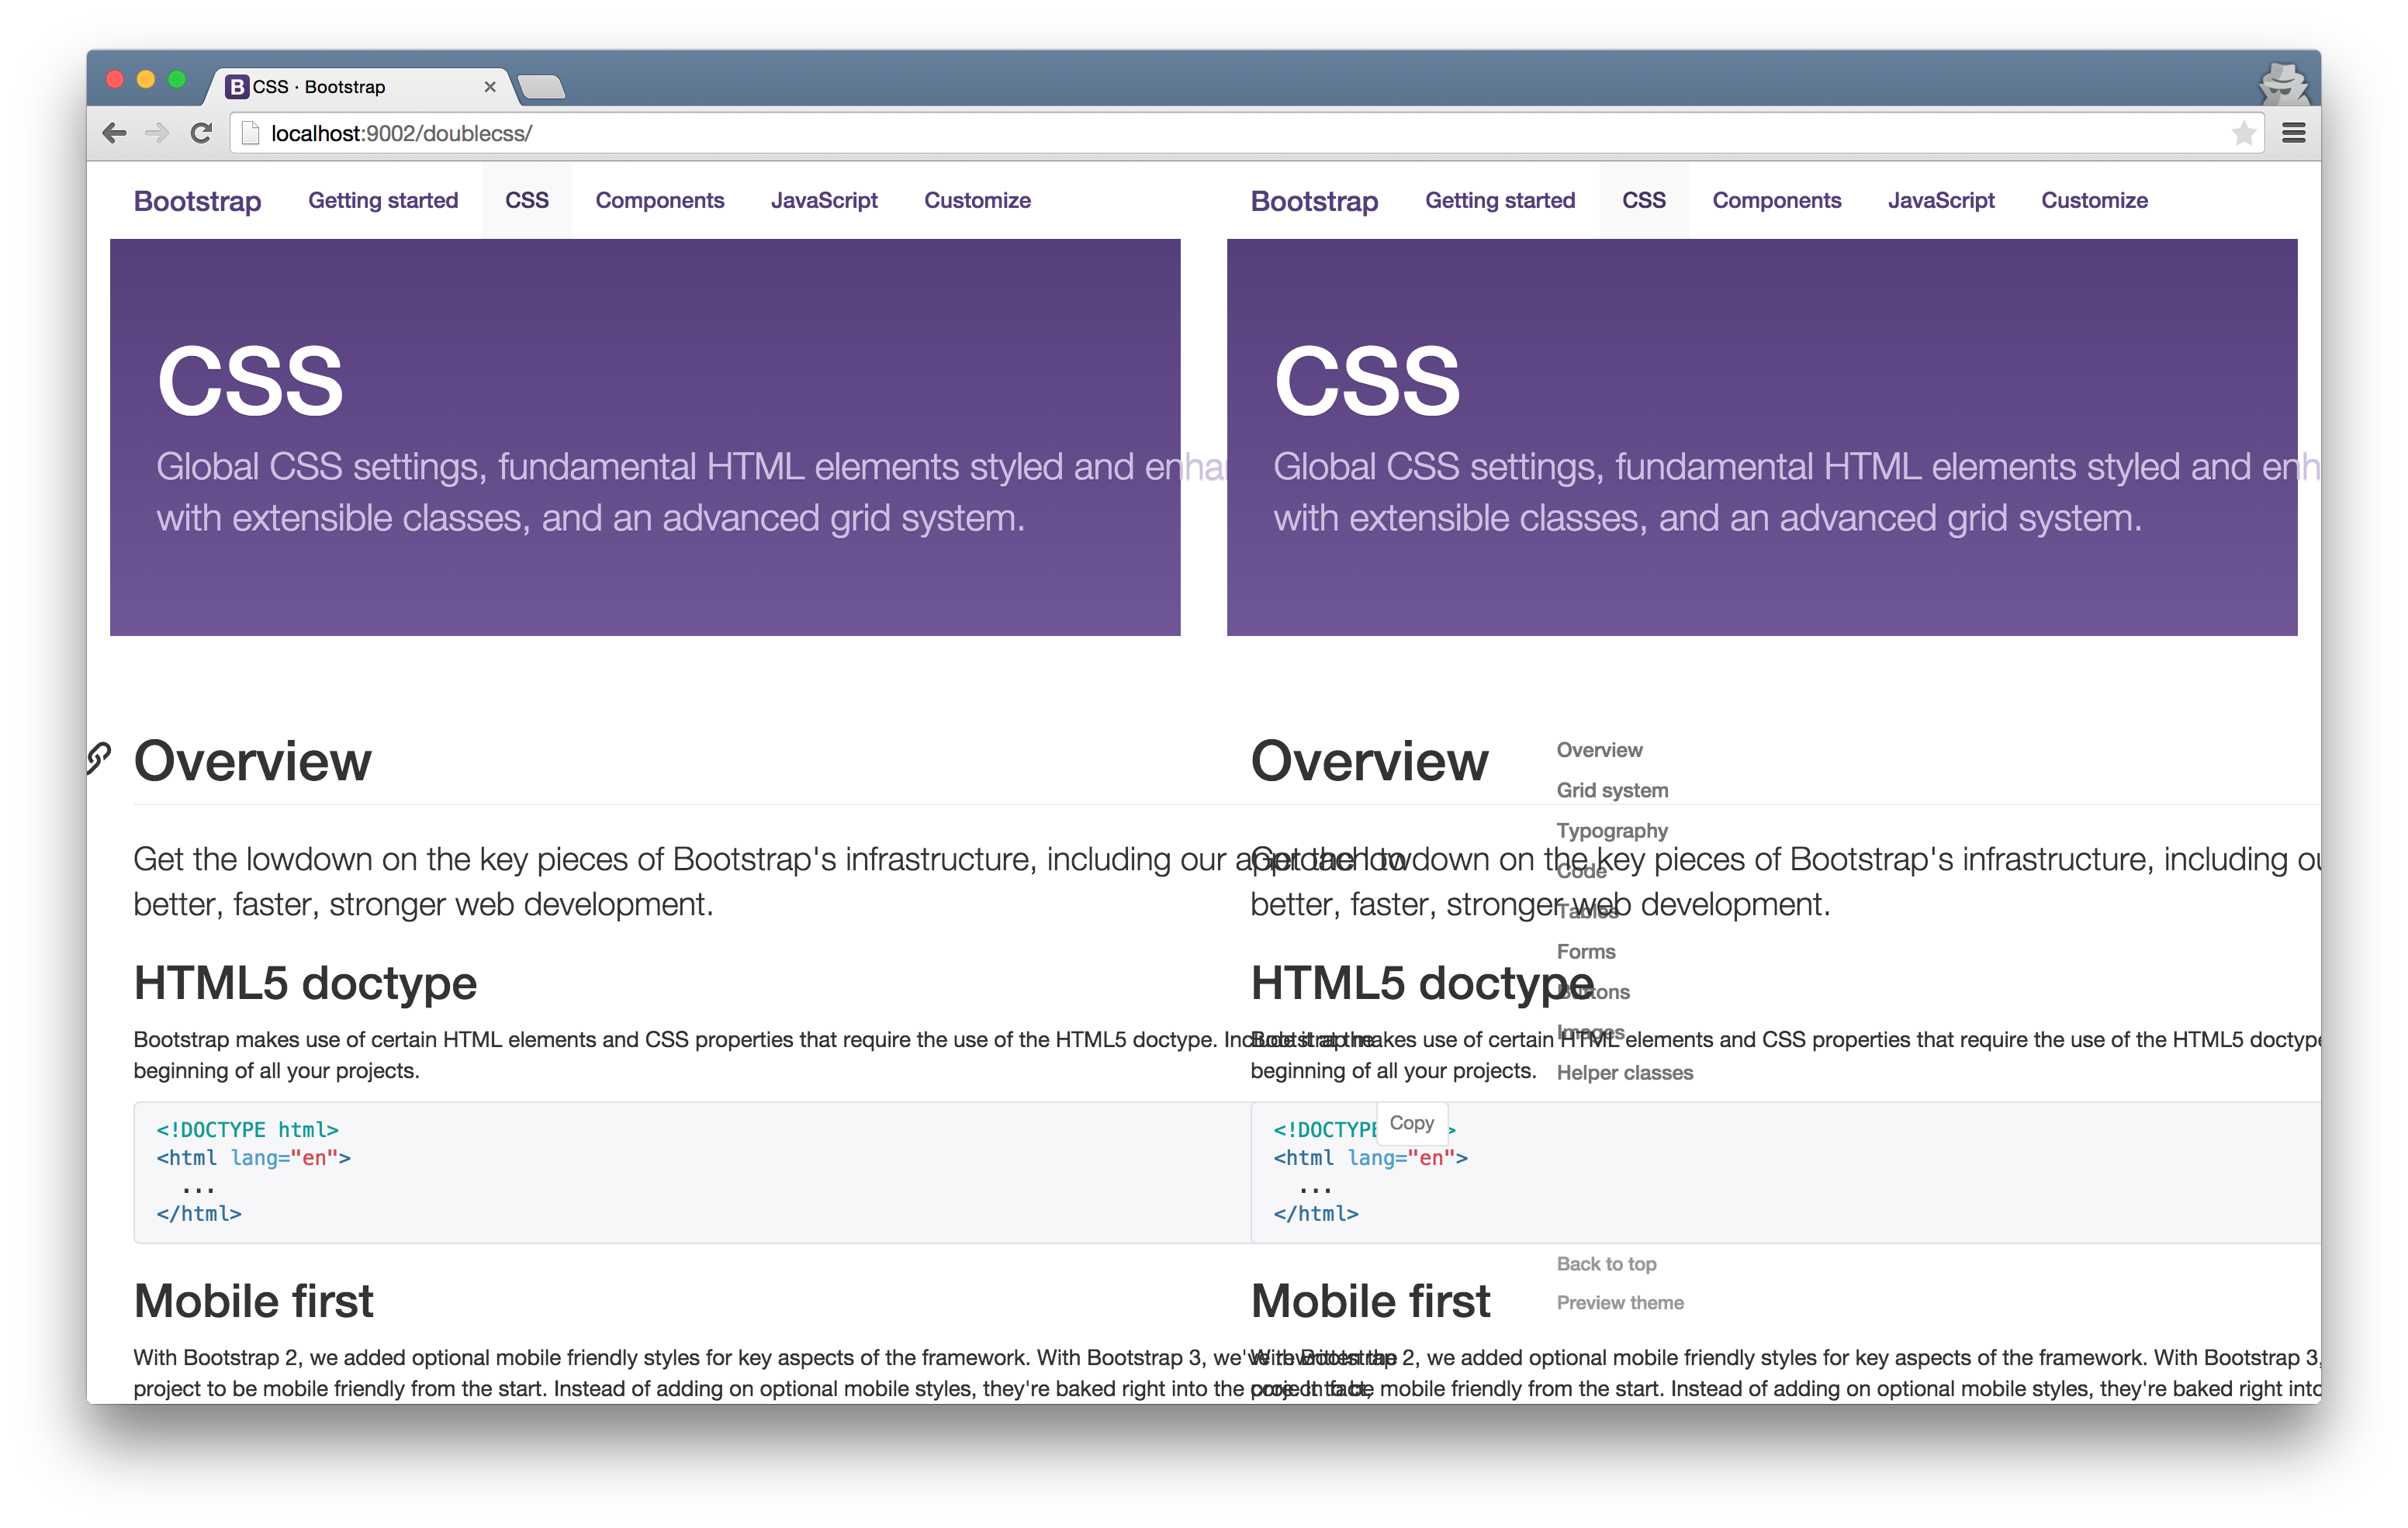
\includegraphics[width=0.9\linewidth]{images/bootstrap-mq-header-small}
          \caption{Double column documentation page powered by \gls{Bootstrap} showing the header section of the page.}
          \label{fig:appendix-bootstrap-mq-header-small}
        \end{figure}
        \begin{figure}[htbp!]
          \centering
          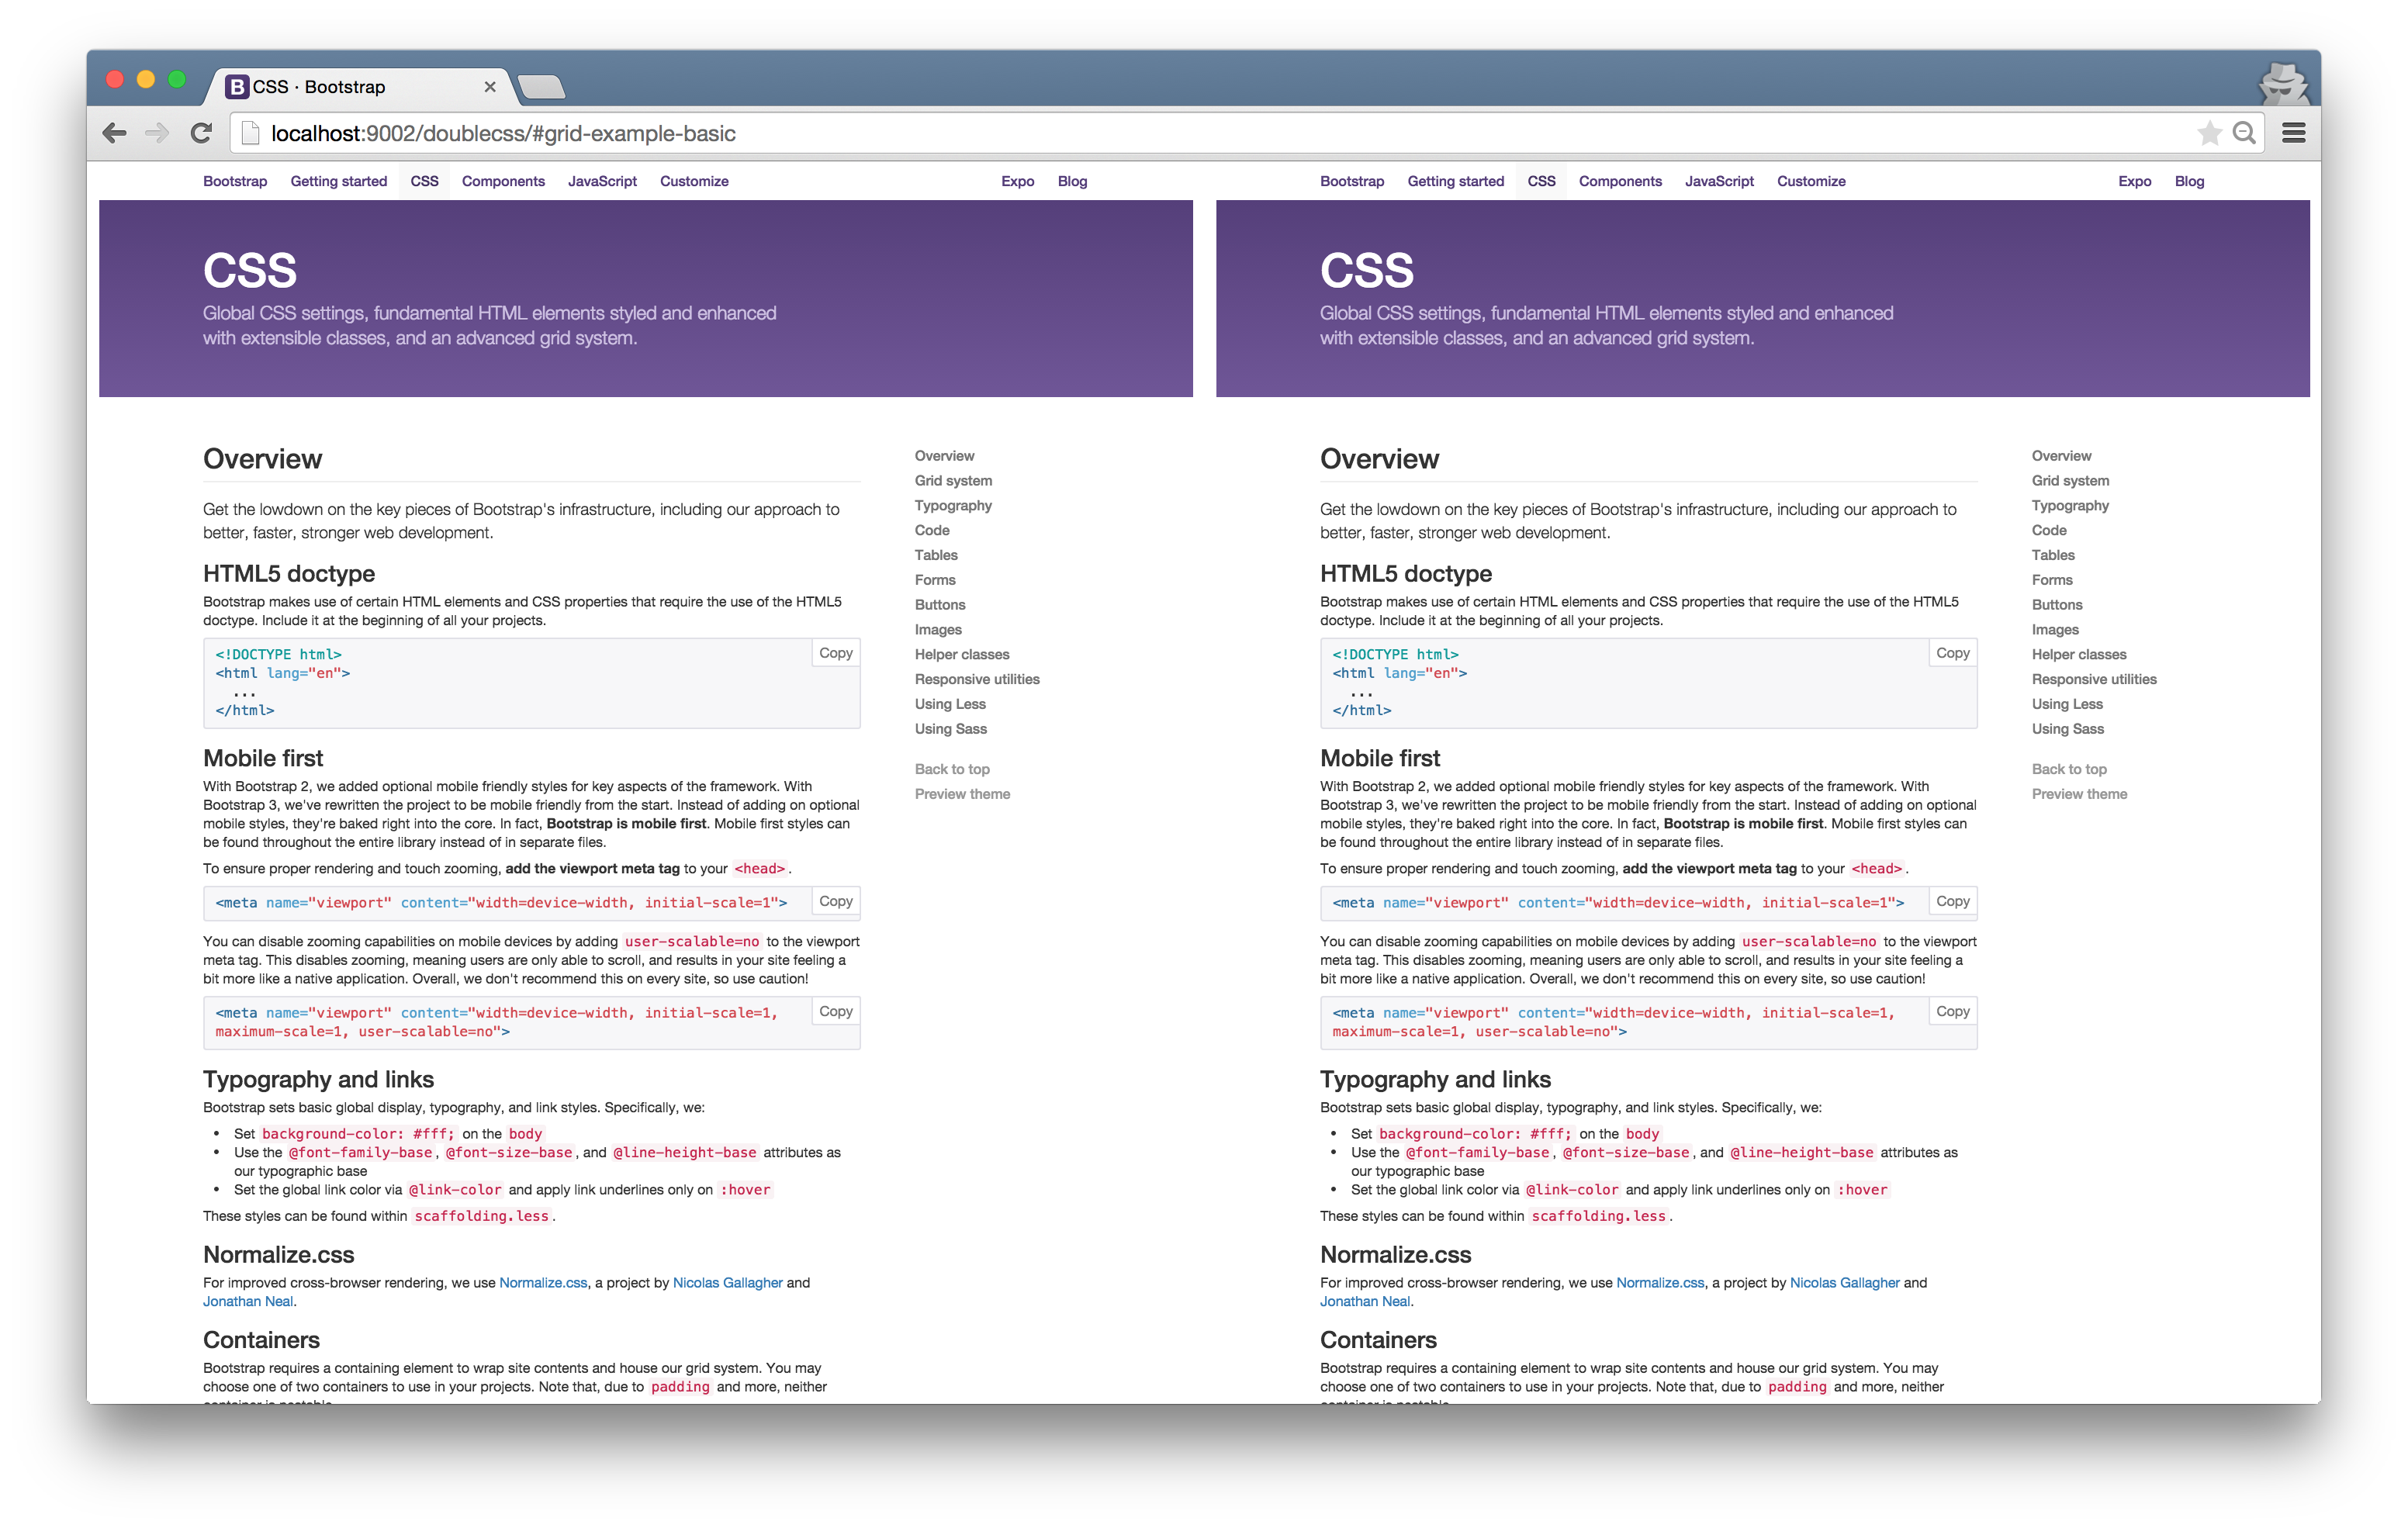
\includegraphics[width=0.9\linewidth]{images/bootstrap-mq-header-big}
          \caption{Double column documentation page powered by \gls{Bootstrap} with showing the header section of the page. The \gls{viewport} is big enough to give each column sufficient space.}
          \label{fig:appendix-bootstrap-mq-header-big}
        \end{figure}

        \begin{figure}[htbp!]
          \centering
          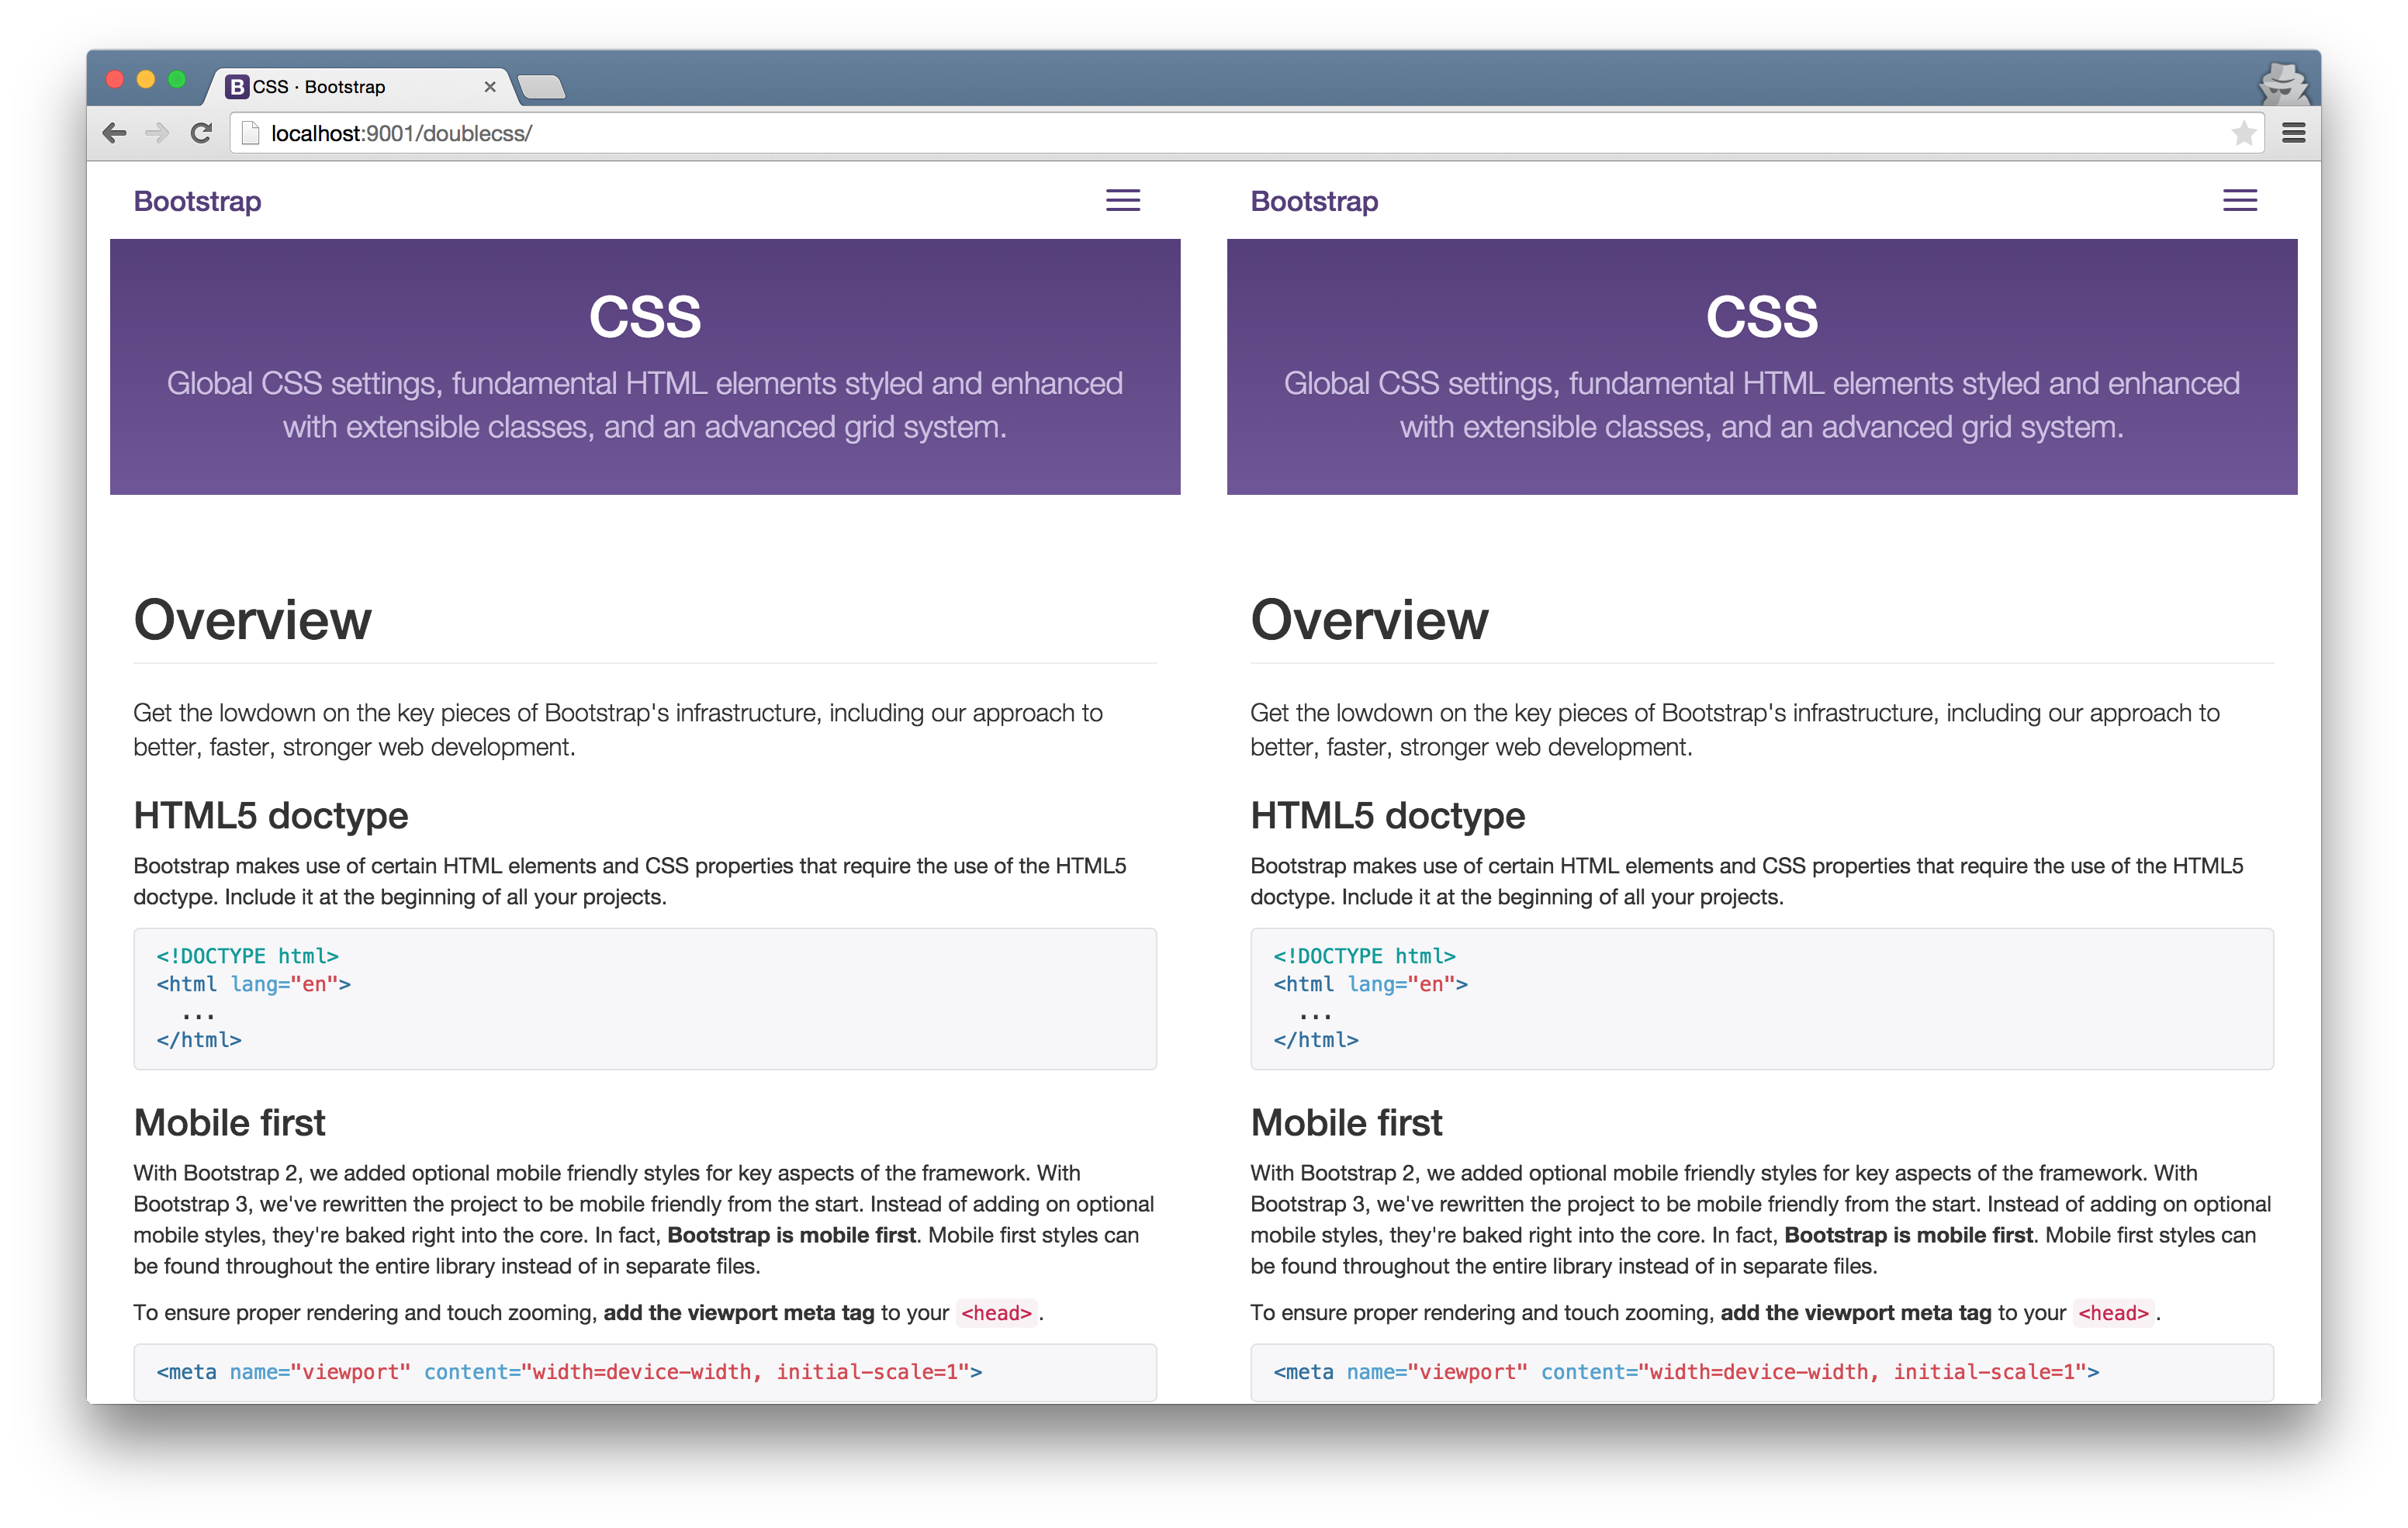
\includegraphics[width=0.9\linewidth]{images/bootstrap-eq-header-small}
          \caption{Double column documentation page powered by \gls{ELQ} \gls{Bootstrap} showing the header section of the page.}
          \label{fig:appendix-bootstrap-eq-header-small}
        \end{figure}

        \begin{figure}[htbp!]
          \centering
          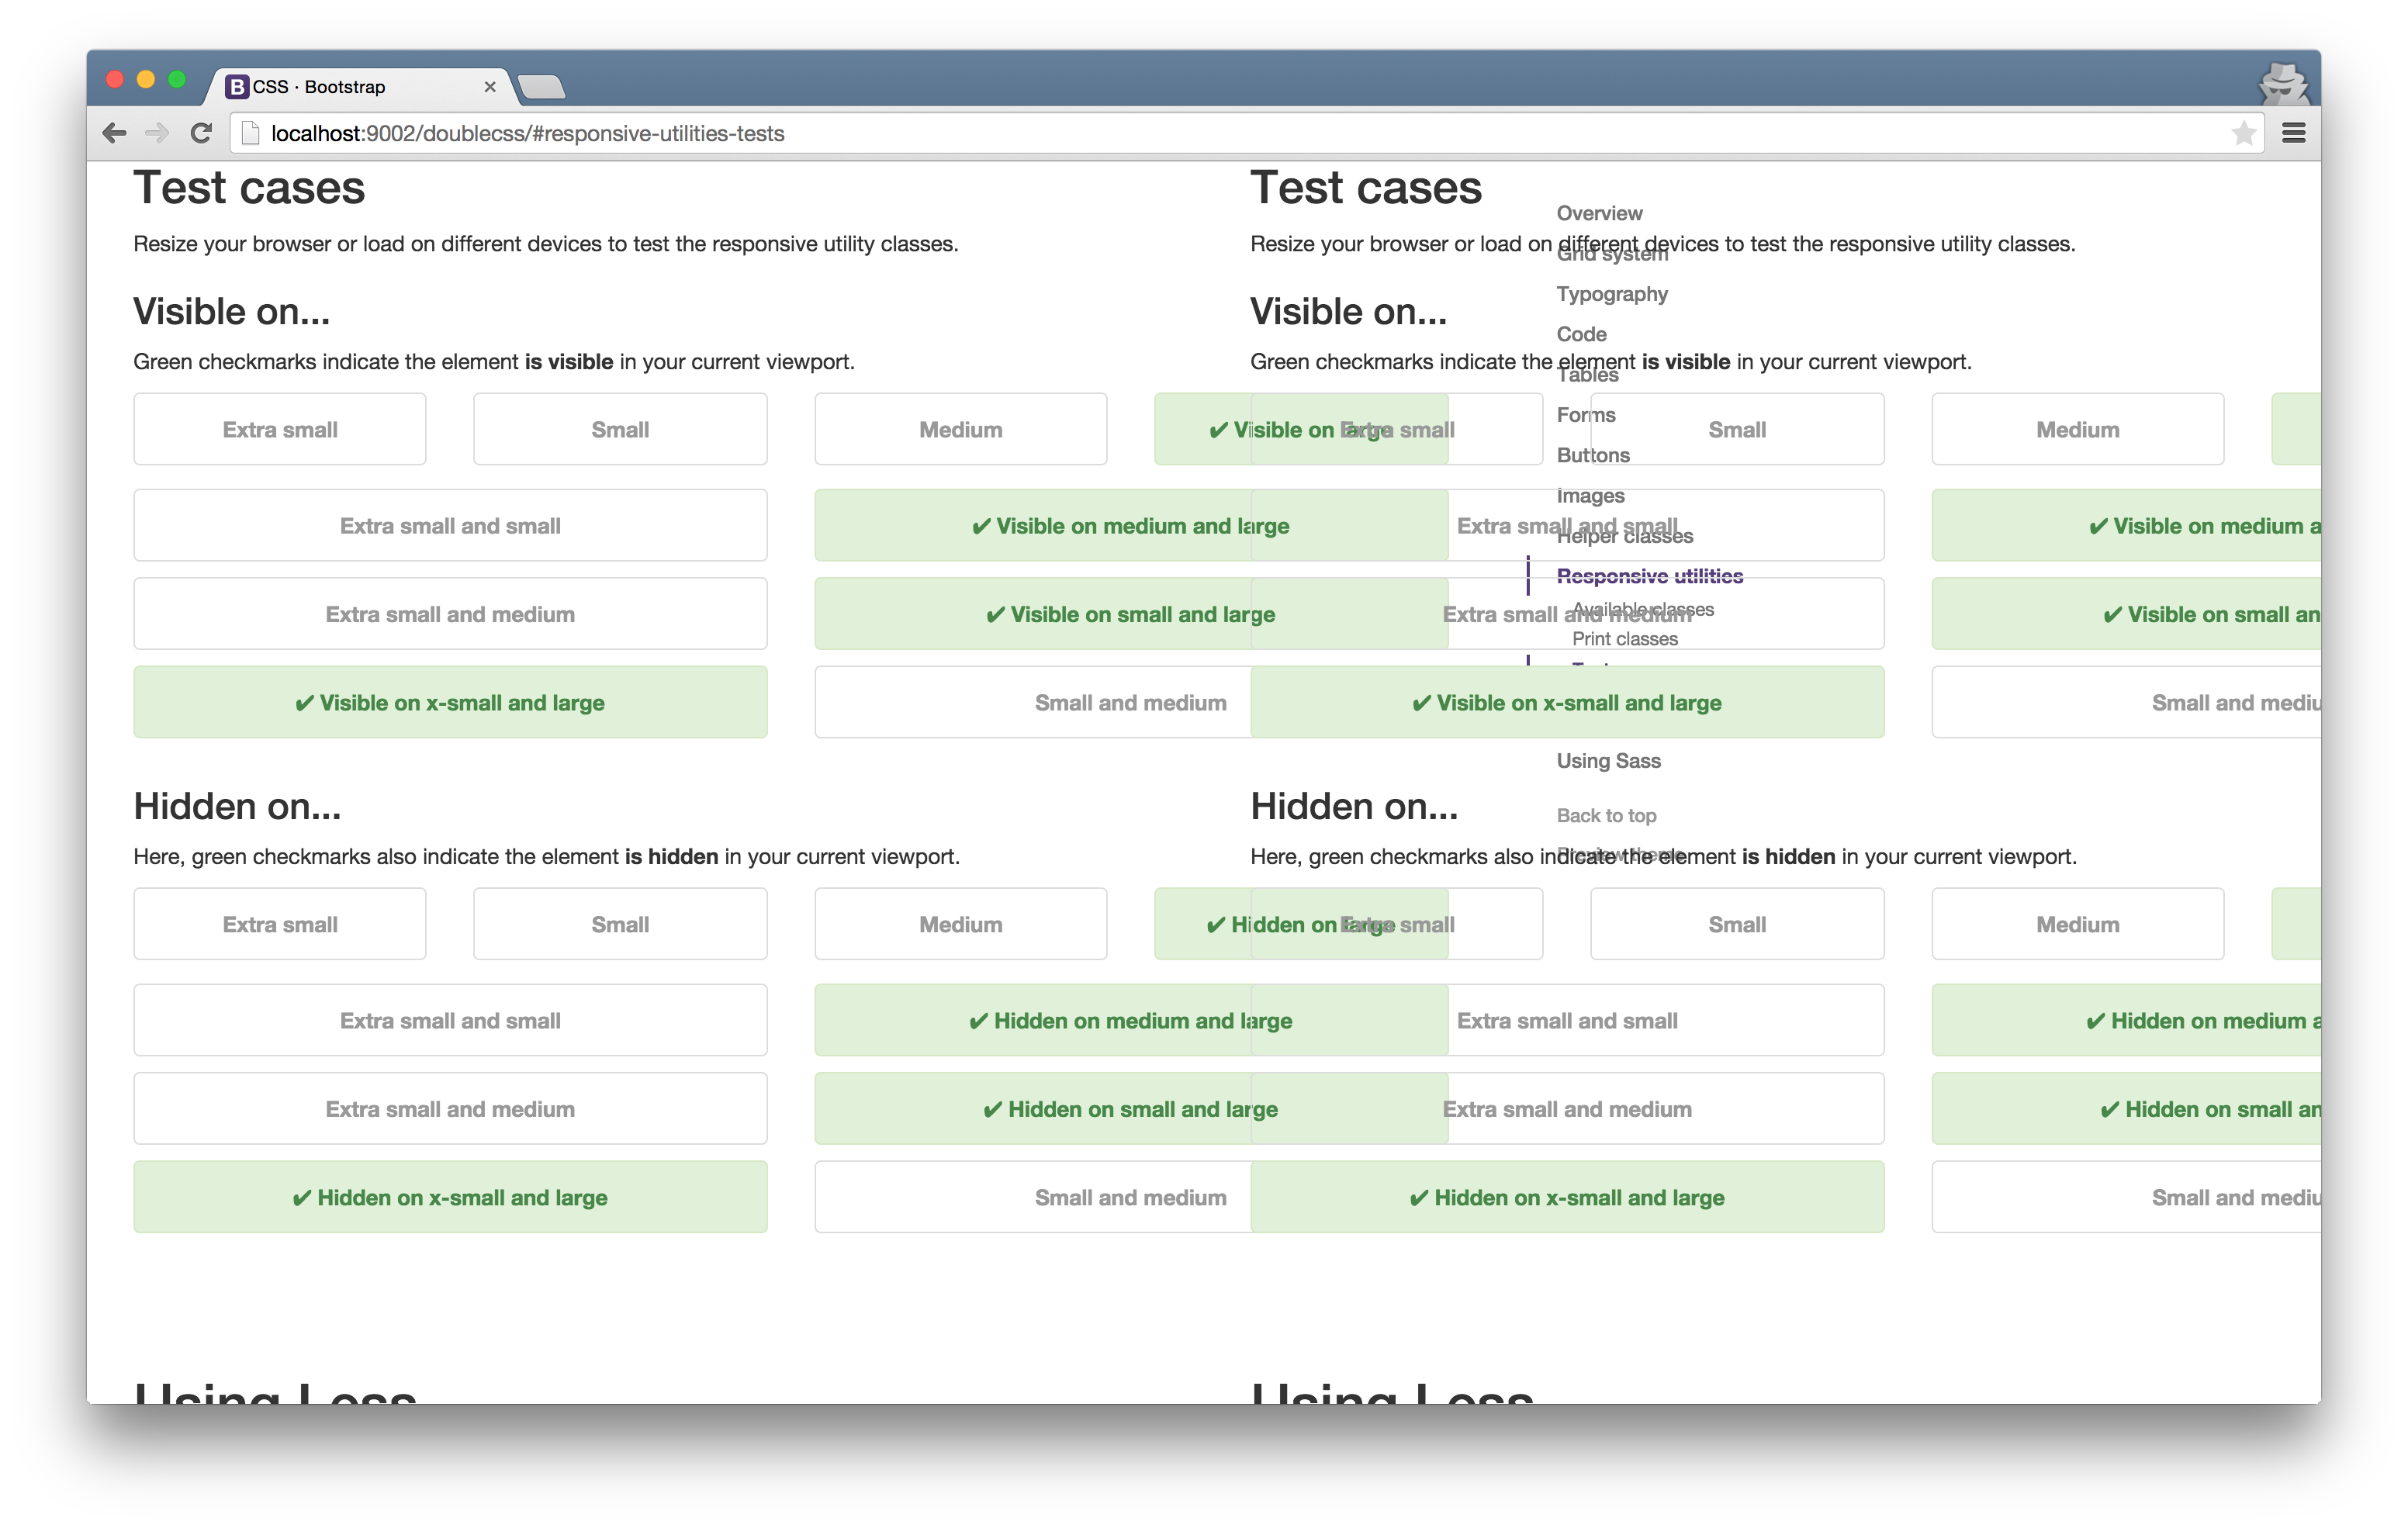
\includegraphics[width=0.9\linewidth]{images/bootstrap-mq-matrix}
          \caption{Double column documentation page powered by \gls{Bootstrap} showing the \gls{responsive} classes matrix section of the page.}
          \label{fig:appendix-bootstrap-mq-matrix-small}
        \end{figure}
        \begin{figure}[htbp!]
          \centering
          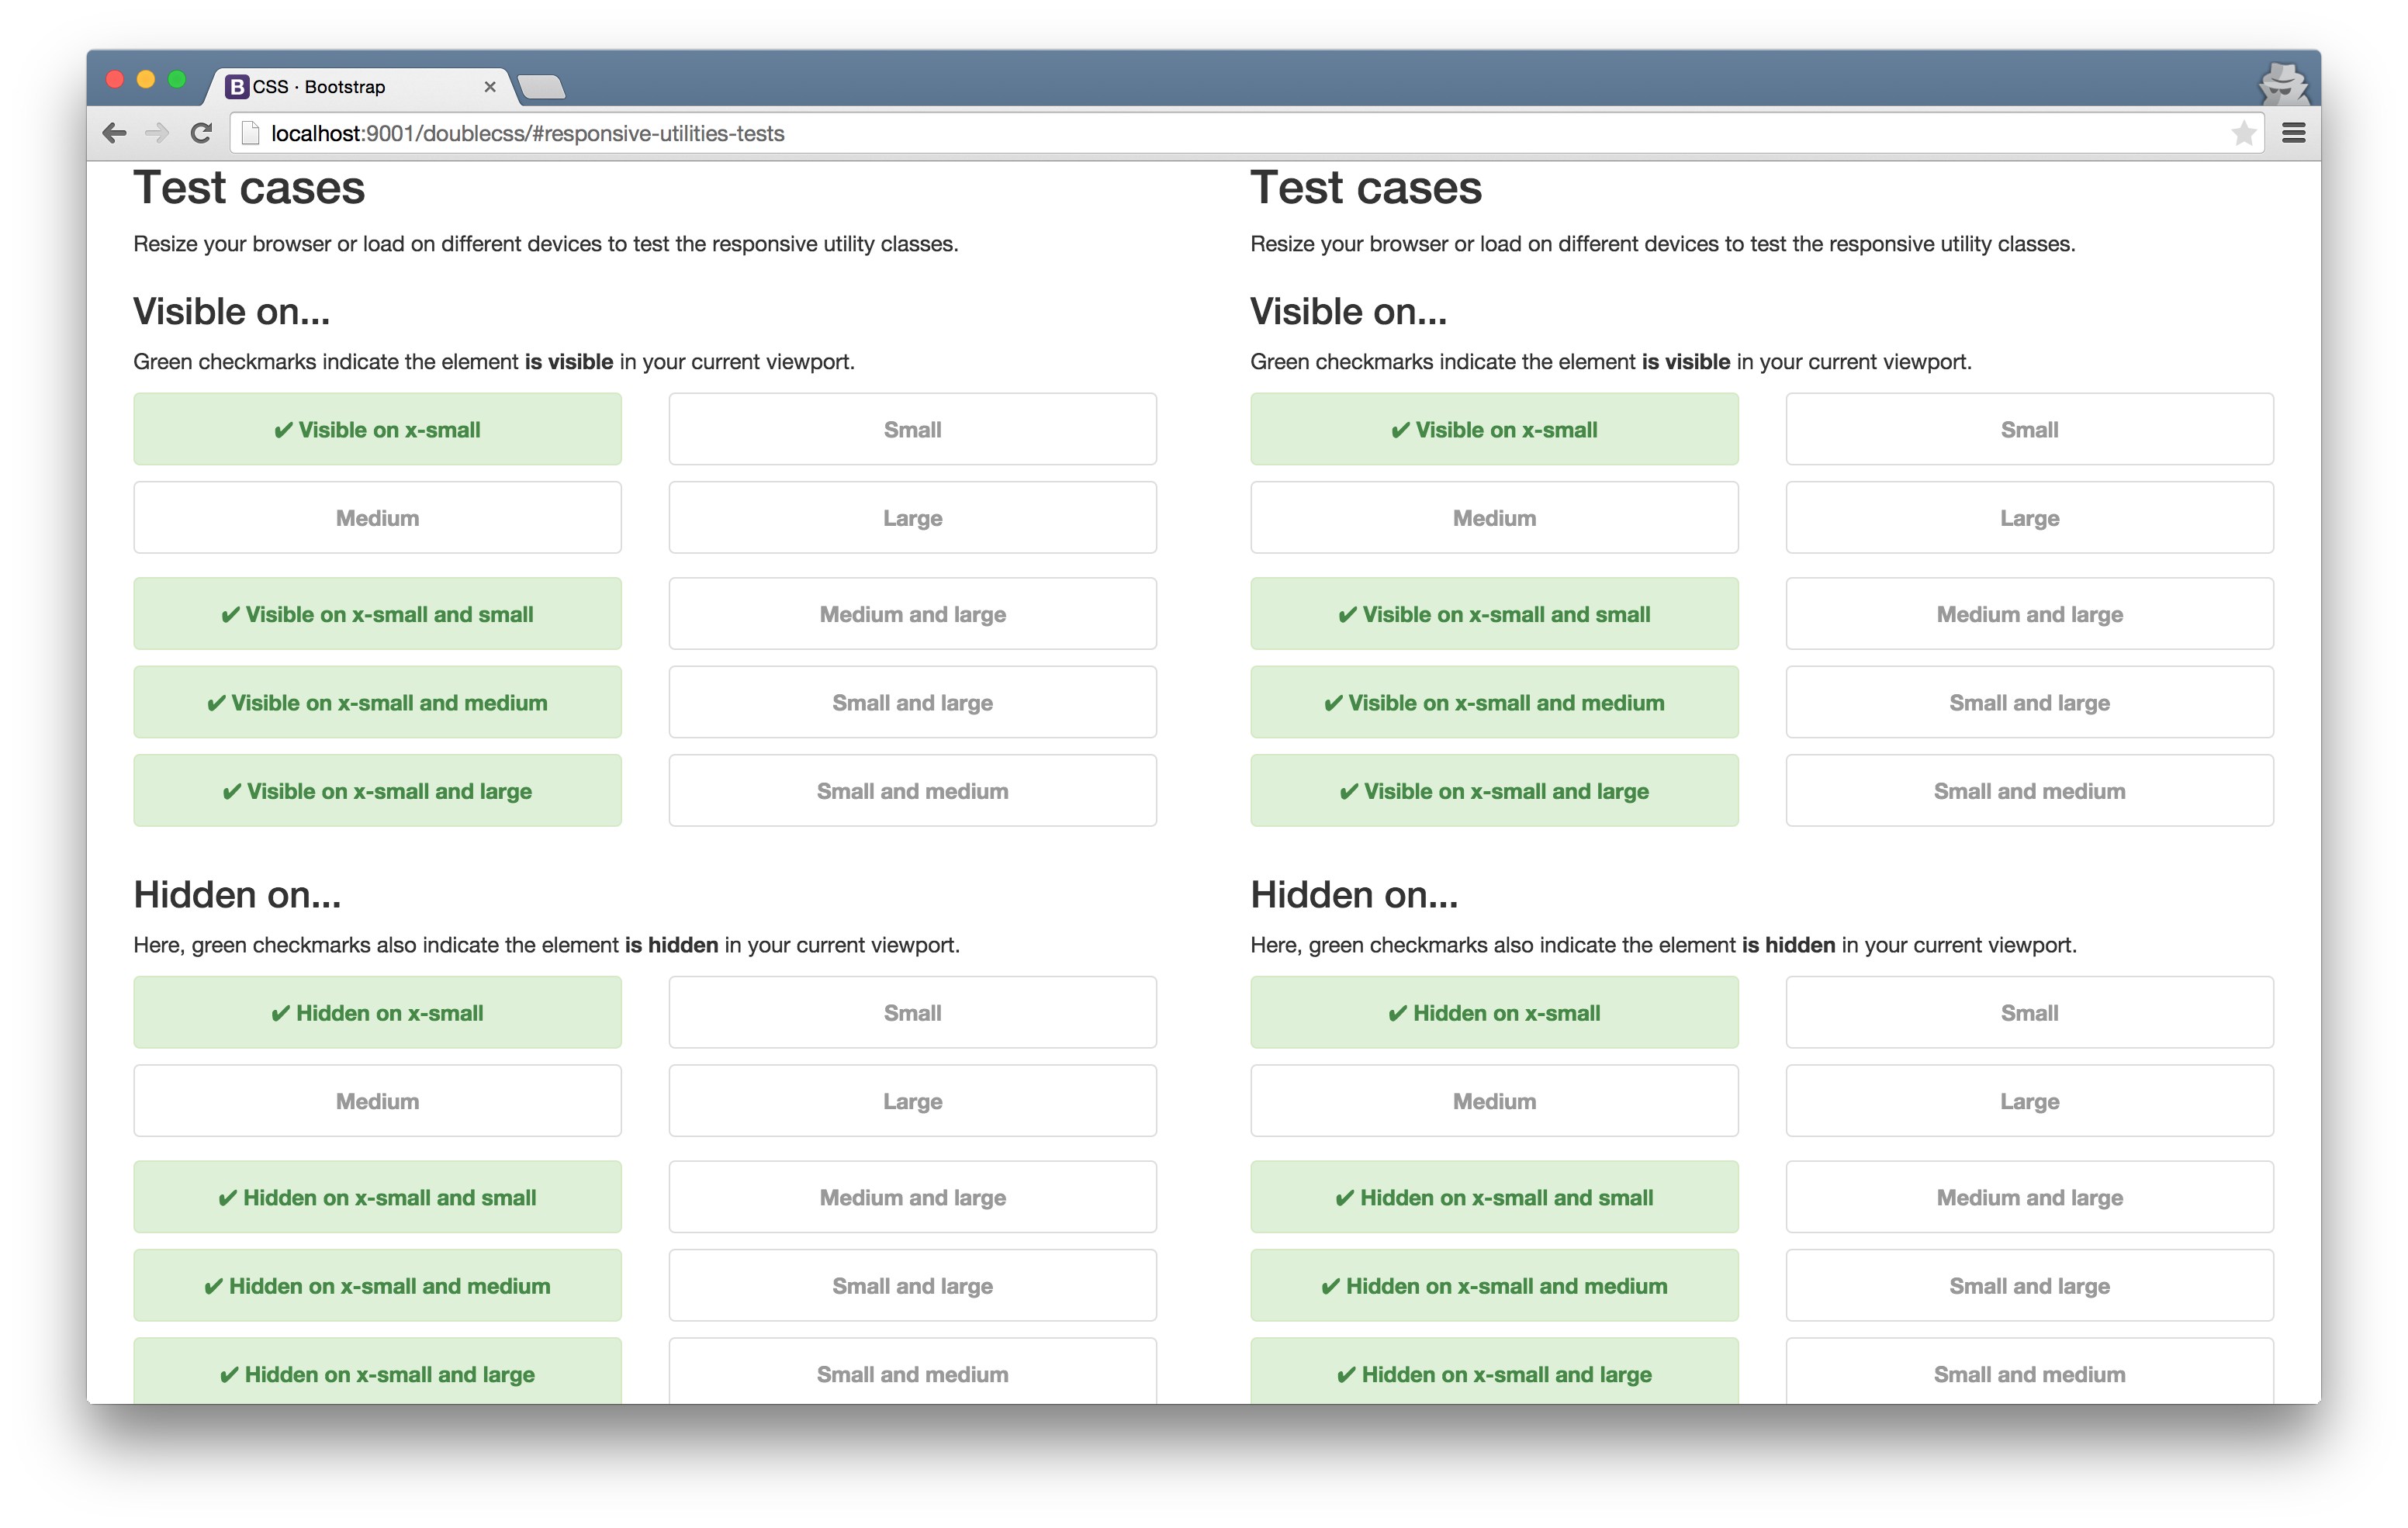
\includegraphics[width=0.9\linewidth]{images/bootstrap-eq-matrix}
          \caption{Double column documentation page powered by \gls{ELQ} \gls{Bootstrap} showing the \gls{responsive} classes matrix section of the page.}
          \label{fig:appendix-bootstrap-eq-matrix-small}
        \end{figure}

        \begin{figure}[htbp!]
          \centering
          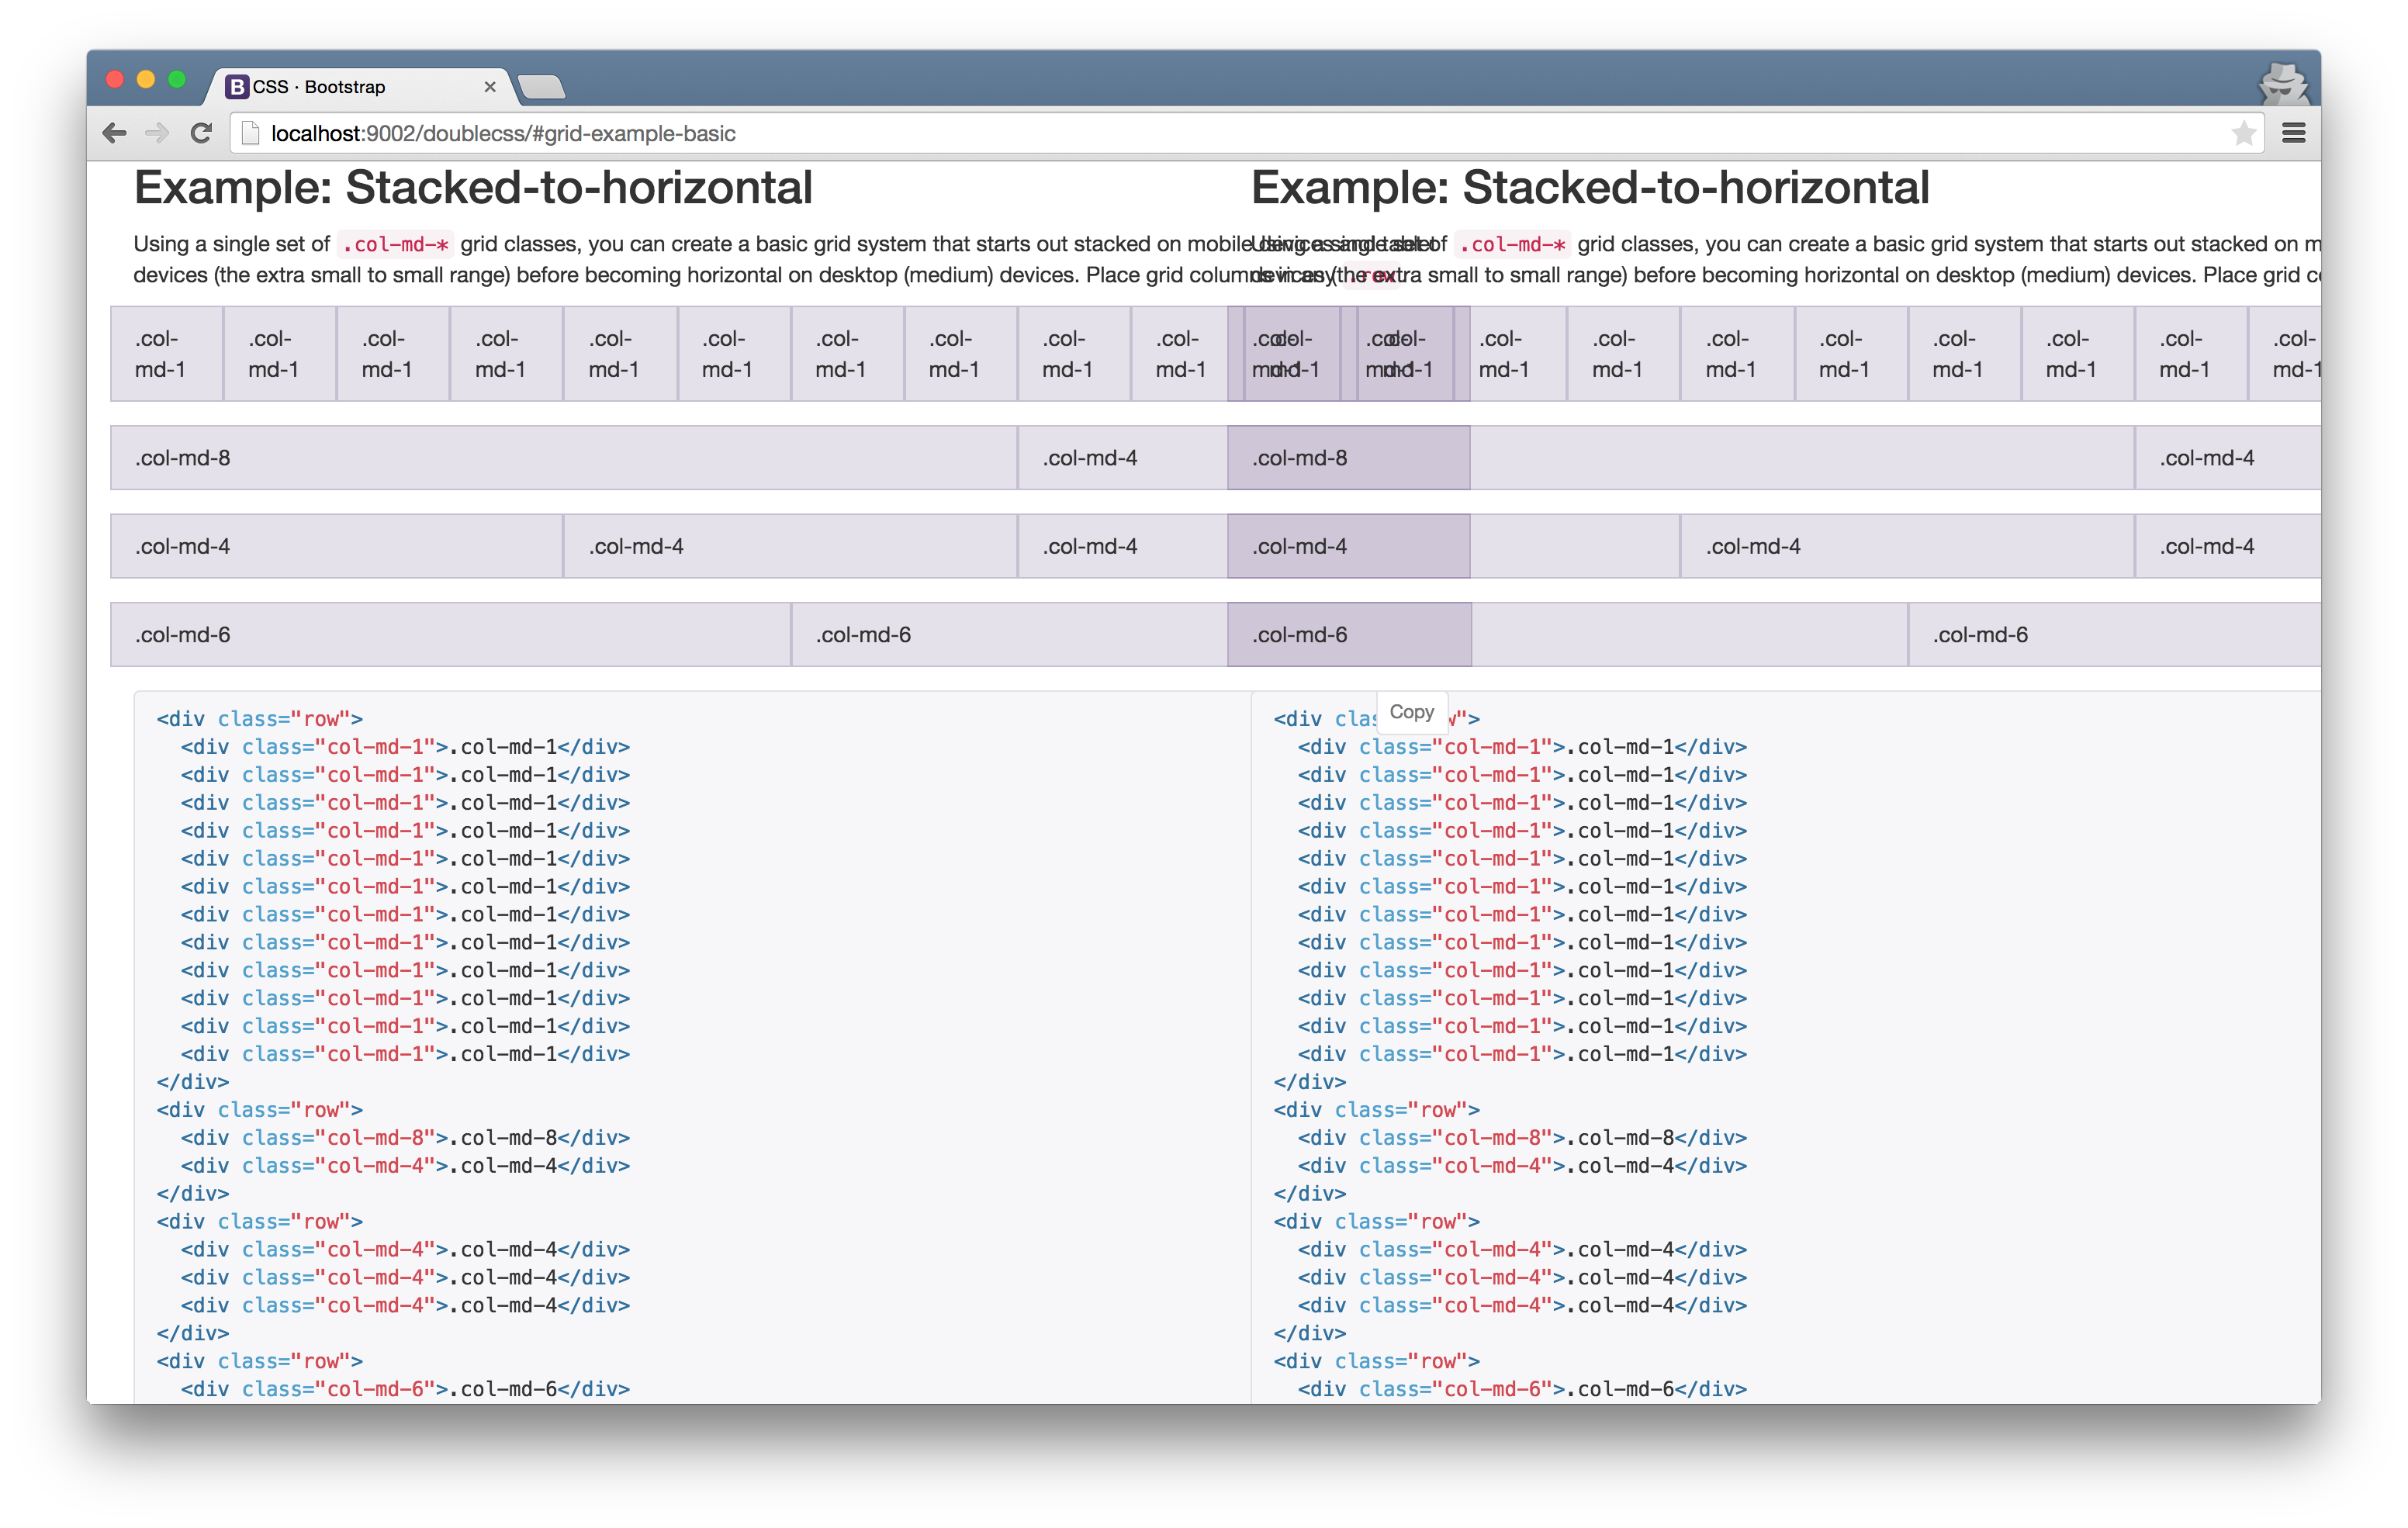
\includegraphics[width=0.9\linewidth]{images/bootstrap-mq-grid}
          \caption{Double column documentation page powered by \gls{Bootstrap} showing the grid section of the page.}
          \label{fig:appendix-bootstrap-mq-grid-small}
        \end{figure}
        \begin{figure}[htbp!]
          \centering
          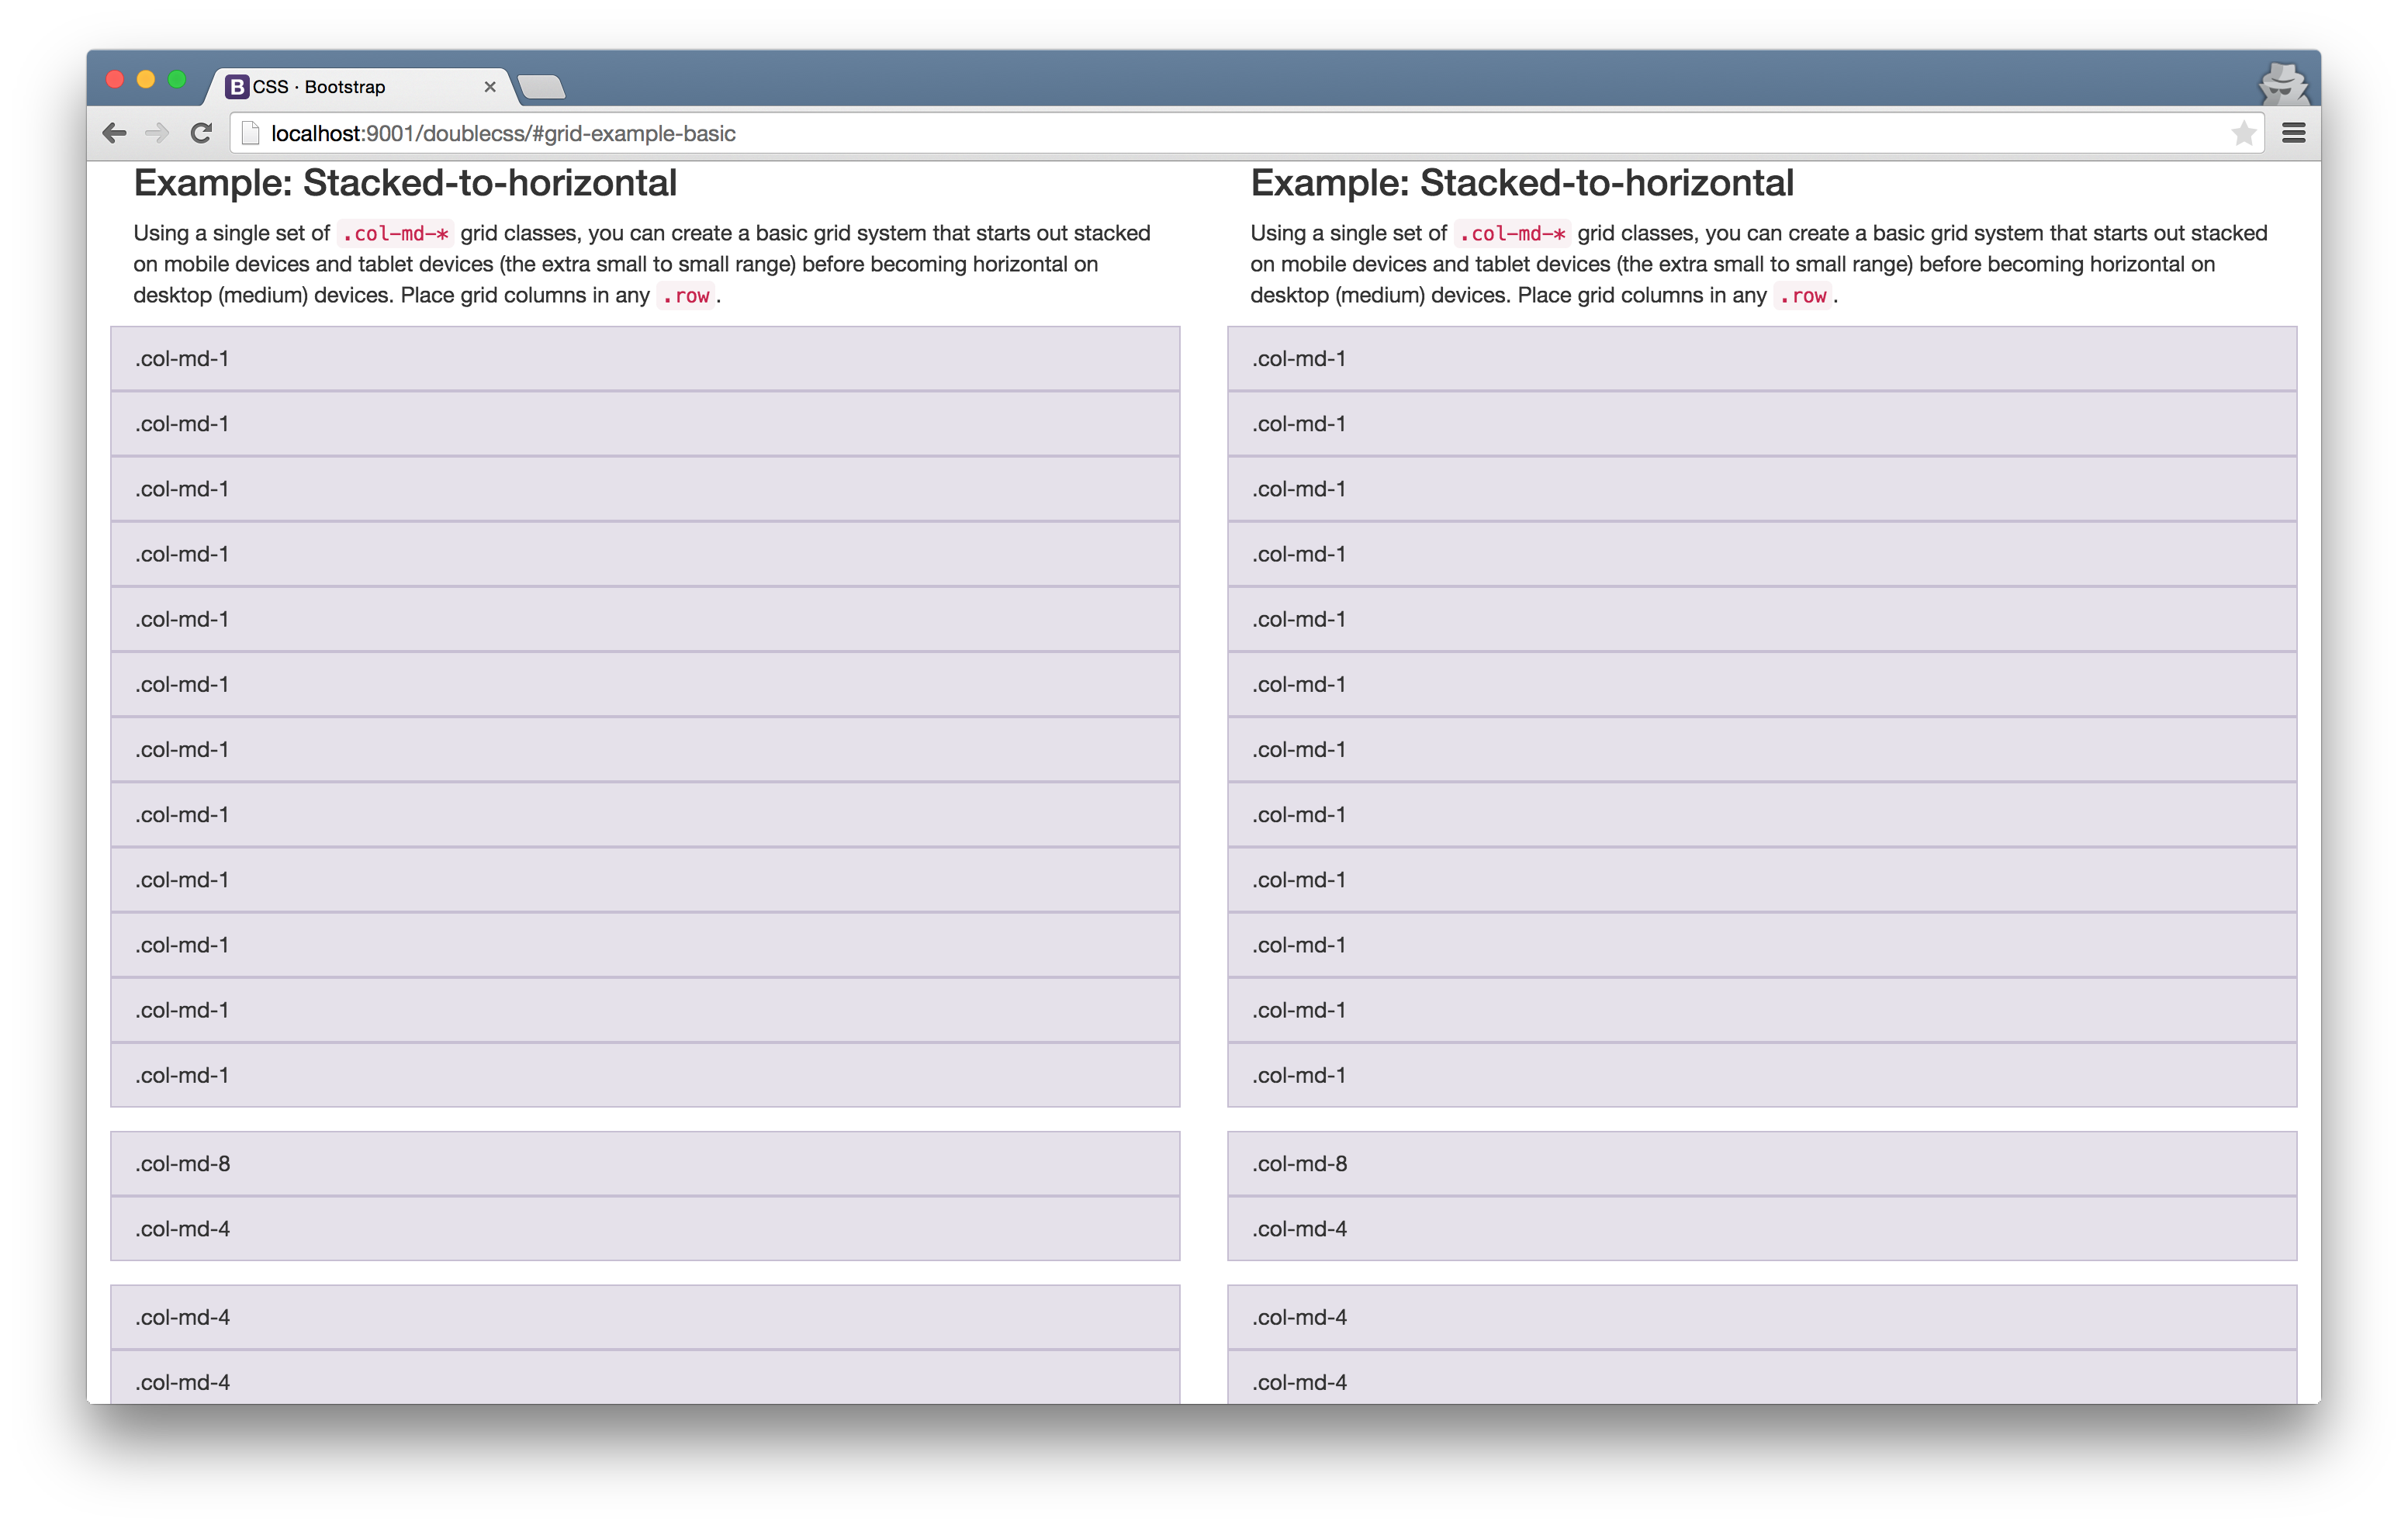
\includegraphics[width=0.9\linewidth]{images/bootstrap-eq-grid}
          \caption{Double column documentation page powered by \gls{ELQ} \gls{Bootstrap} showing the grid section of the page.}
          \label{fig:appendix-bootstrap-eq-grid-small}
        \end{figure}

        \FloatBarrier
      \section{Layout engine market share statistics}\label{sec:layout_engines_market_share}
        \Gls{browser} market share was retrieved by \gls{StatCounter}\footnote{\gls{StatCounter} graph \url{http://gs.statcounter.com/\#all-browser-ww-monthly-201402-201502-bar}}.
        Since the graph only display \gls{browser} market share and not \gls{layout engine}, it is needed to further divide the \glspl{browser} into \gls{layout engine} percentages.
        The \gls{Blink} engine was introduced with Chrome version 28 and Android version 4.4 \cite{wiki_blink}.
        Since Chrome has very good adoption rate\footnote{According to \url{http://clicky.com/marketshare/global/web-browsers/google-chrome/}} of new versions the Chrome market share percentage of 39.72\% is considered to be \gls{Blink} based.
        However, Android has not as good adoption rate as Chrome with only 44.2\% using Android version 4.4 and up\footnote{According to \url{https://developer.android.com/about/dashboards/index.html}}.
        Android has a \gls{browser} market share of 7.21\%. 44.2\% of the 7.21\% Android \glspl{browser} is assumed to be \gls{Blink} based and 55.8\% to be \gls{WebKit} based (since the Android \gls{browser} was \gls{WebKit} based before \gls{Blink}).
        Of course, the assumption that users with old versions of Android browse the {\gls{web} as much as users with new versions are probably invalid, but the data source itself is uncertain enough to make such assumptions and the percentages should only be regarded as guidelines.
        Opera with the lowest market share at 3.97\% started using the \gls{Blink} engine in late 2013 as of version 15.
        \gls{StatCounter} shows that 37\% of the Opera users are using Opera Mini (their mobile \gls{browser}), which does not use the \gls{Blink} engine (it uses Opera's own Presto \gls{layout engine} which will be ignored).
        All desktop users of Opera are assumed to be using version 15 or above and hence using the \gls{Blink} engine.
        The total market share percentage of the \gls{Blink} engine is then calculated to $39.72 + 0.442\cdot7.21 + 0.37\cdot3.97 = 44.38\%$.
        Safari, with the market share percentage of 7.46\%, has always been \gls{WebKit} based.
        iOS also uses \gls{WebKit} and has the market share percentage of 6.16\%.
        The \gls{WebKit} market share percentage is calculated to $7.46 + 0.558\cdot7.21 + 6.16 = 17.64\%$.
        FireFox, with the market share percentage of 12.83\%, has always been \gls{Gecko} based and is the only major \gls{browser} that uses the \gls{Gecko} engine.
        The market share percentage of \gls{Gecko} is therefore 12.83\%.
        Internet Explorer, with the market share percentage of 14.96\%, has been \gls{Trident} based since version 4.
        Since Internet Explorer 4 is no longer in use\footnote{According to \url{http://www.w3schools.com/browsers/browsers_explorer.asp}}, the market share percentage of the \gls{Trident} engine is 14.96\%.
      % TODO: Write this?
      % \section{Usage share of browser versions}
      %   \todo{Put this somewhere else?}
      %   For compatibility, the library needs to support older \glspl{browser}.
      %   Most of the end users are using a self updating \gls{browser} (those \glspl{browser} are usually referred to as the \emph{evergreen} \glspl{browser}), which improves the adoption rate of new versions greatly.
      %   See figure~\todo{Have a figure or not? If yes, then reference it here.} for the adoption rate of new versions of Chrome for an example of how evergreen \glspl{browser} keep their users updated.
      %   Unfortunately, there are some laggards that still use very outdated versions of some \glspl{browser}.
      %   Each version of Internet Explorer 8 up to 11 need to be supported since they all still have a significant user share.
      %   Opera version 12 does also have
\end{document}
